% !TeX program = pdflatex
% !BIB program = biber

\documentclass[11pt,a4paper]{article}

% PREAMBLE
\usepackage[margin=1in]{geometry}
\usepackage{graphicx,booktabs,amsmath,amssymb,mathtools,float}
\usepackage{siunitx}\sisetup{detect-all}
\usepackage[hidelinks]{hyperref}
\usepackage{titlesec}
\usepackage{tocloft}
\usepackage{newtxtext,newtxmath} % Times New Roman
\usepackage{tabularx}
\usepackage{subfiles}
\usepackage{amsmath}

% TabularX Parameters
\newcolumntype{Y}{>{\raggedright\arraybackslash}X}

\setlength{\parindent}{20pt}

% TOC Depth
\setcounter{secnumdepth}{5}
\setcounter{tocdepth}{5}

% Section Numbering
\renewcommand\thesection{\arabic{section}}
\renewcommand\thesubsection{\thesection.\arabic{subsection}}
\renewcommand\thesubsubsection{\thesubsection.\arabic{subsubsection}}

\makeatletter
\renewcommand\theparagraph{\thesubsubsection.\roman{paragraph}}
\makeatother

\titleformat{\paragraph}[hang]{\normalfont\normalsize\bfseries}{\theparagraph}{1em}{}
\titlespacing*{\paragraph}{0pt}{0.75ex}{0.5ex}

% TOC Indentation (skip paragraph due to MiKTeX compatibility)
\setlength{\cftsubsecindent}{1.5em}
\setlength{\cftsubsubsecindent}{3em}

% BEGIN DOCUMENT 
\begin{document}

% Title Page
\begin{titlepage}
    \centering
    {\Huge\bfseries UCSD MAS WES268B - Lab 7 Report\par}
    \vspace{2cm}
    {\large\bfseries 21FEB2025\par}
    \vspace{2cm}
    
\includegraphics[width=0.35\textwidth]{UCSD.png}\par\vspace{1.5cm}
    %\vfill
    \vspace{3cm}
    {\scshape Prepared By: \par}
    {\Large\itshape Joshua Hoang \\ Ryan Shimizu\par}

    % Good Boy Brady
    \vspace*{\fill}
    \hfill
    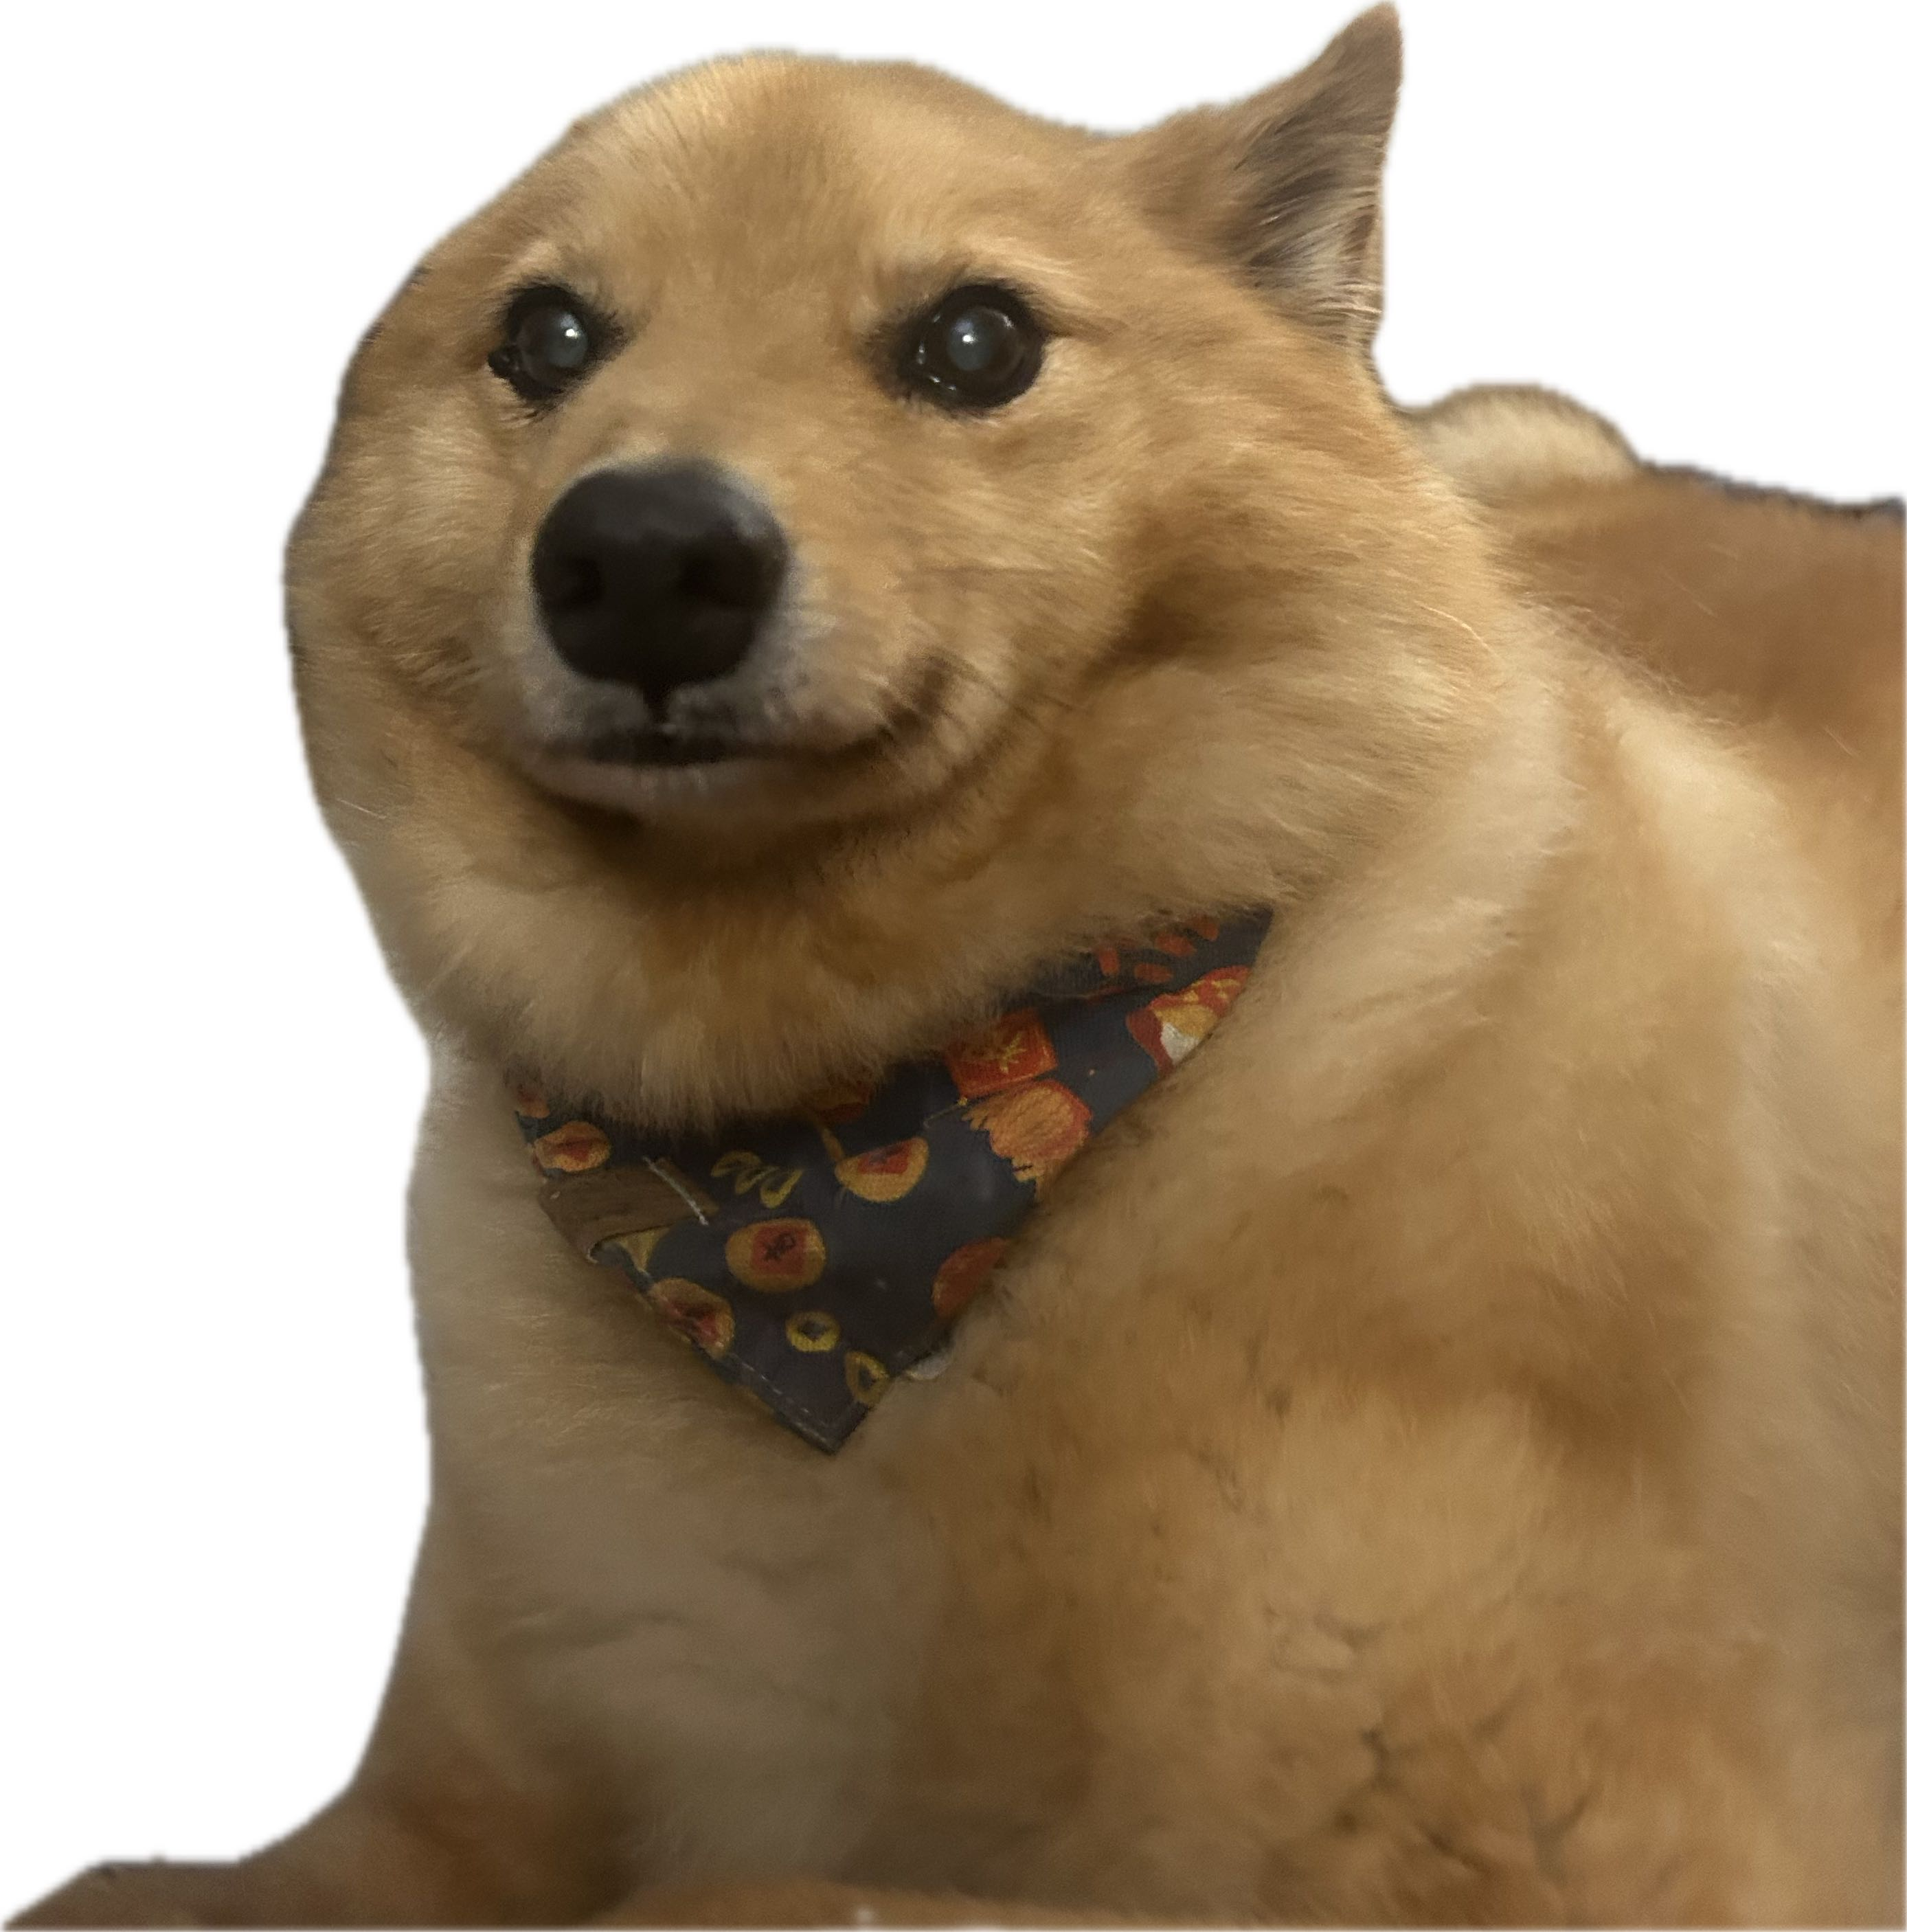
\includegraphics[width=0.2\textwidth]{EasterEgg.png}
\end{titlepage}

% Reset page number after title
\clearpage
\setcounter{page}{2}

% Table of Contents 
\tableofcontents
\newpage

% 1 Coding and Frequency-Selective Fading
\section{Coding and Frequency-Selective Fading}

\subsection{Coding Across Subcarriers}

% 1.1.2
\subsubsection{ }
\begin{figure}[H]
    \centering
    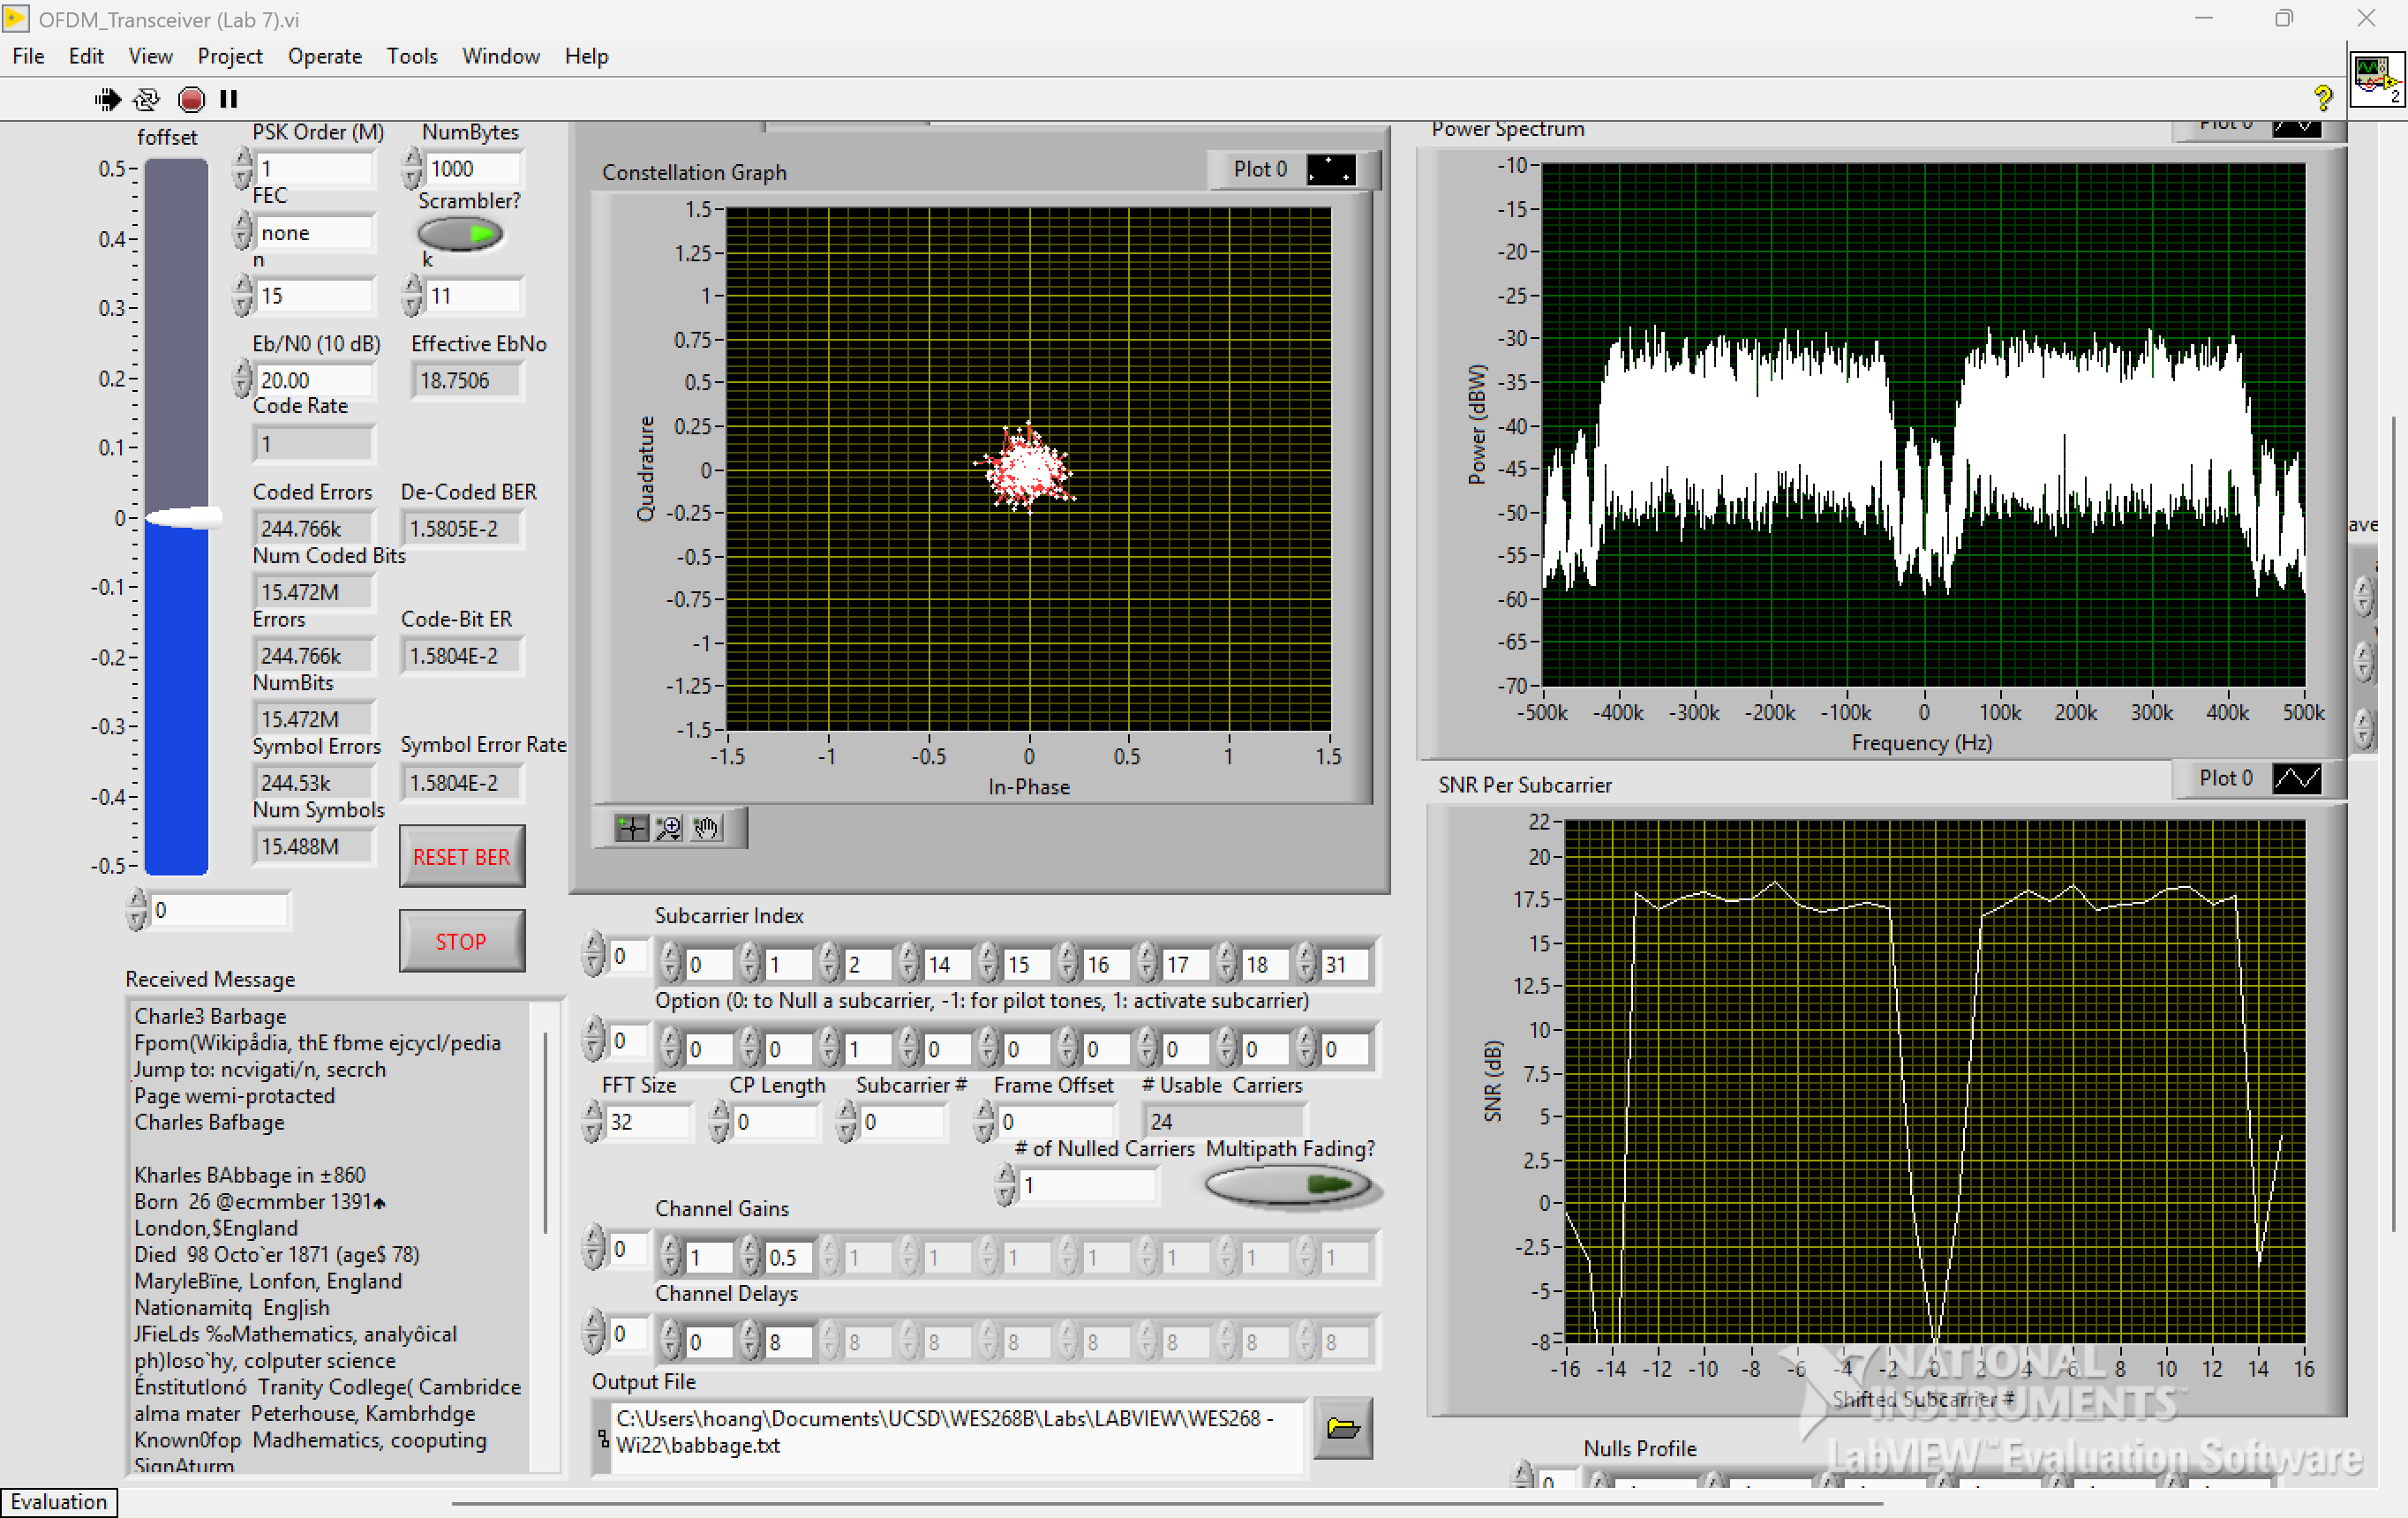
\includegraphics[width=0.7\textwidth]{lab_ss/WES268B_Lab7_Part1-1-2_FEC-None_nullCarriers-1.png}
    \caption{Lab 7 - 1 Nulled Subcarrier}
    %\label{f1}
\end{figure}

\begin{figure}[H]
    \centering
    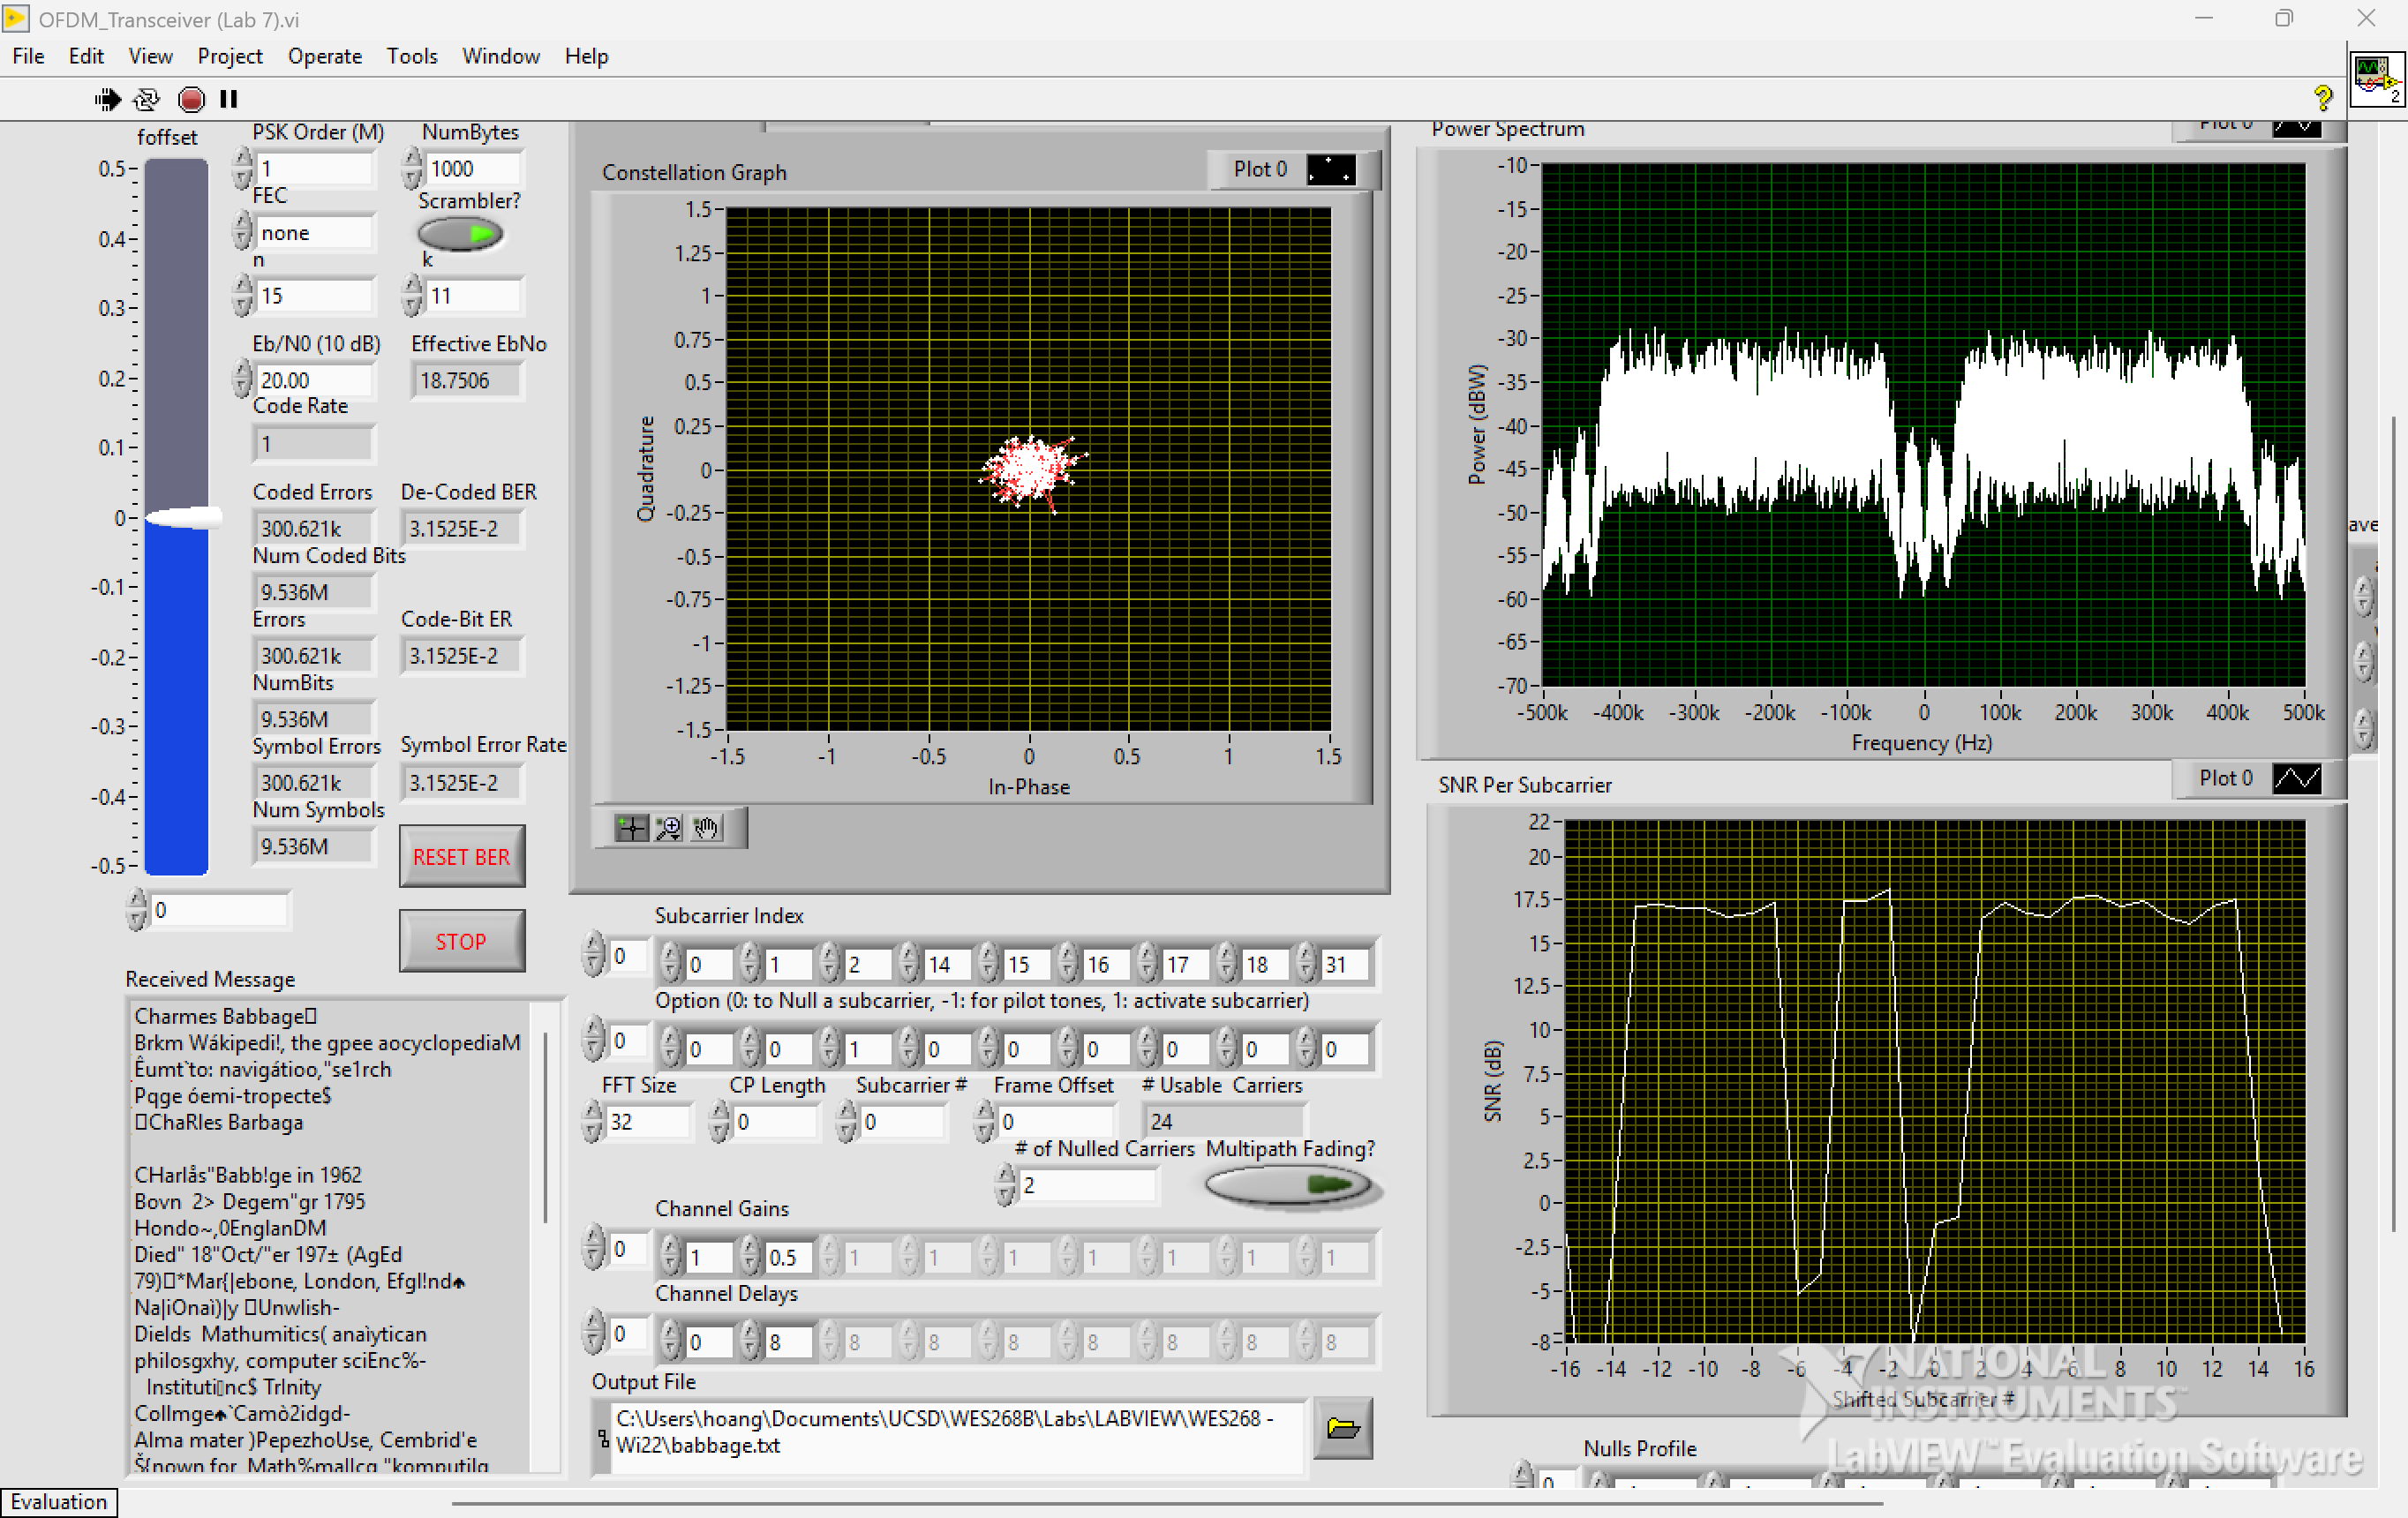
\includegraphics[width=0.7\textwidth]{lab_ss/WES268B_Lab7_Part1-1-2_FEC-None_nullCarriers-2.png}
    \caption{Lab 7 - 2 Nulled Subcarriers}
    %\label{f2}
\end{figure}

\begin{figure}[H]
    \centering
    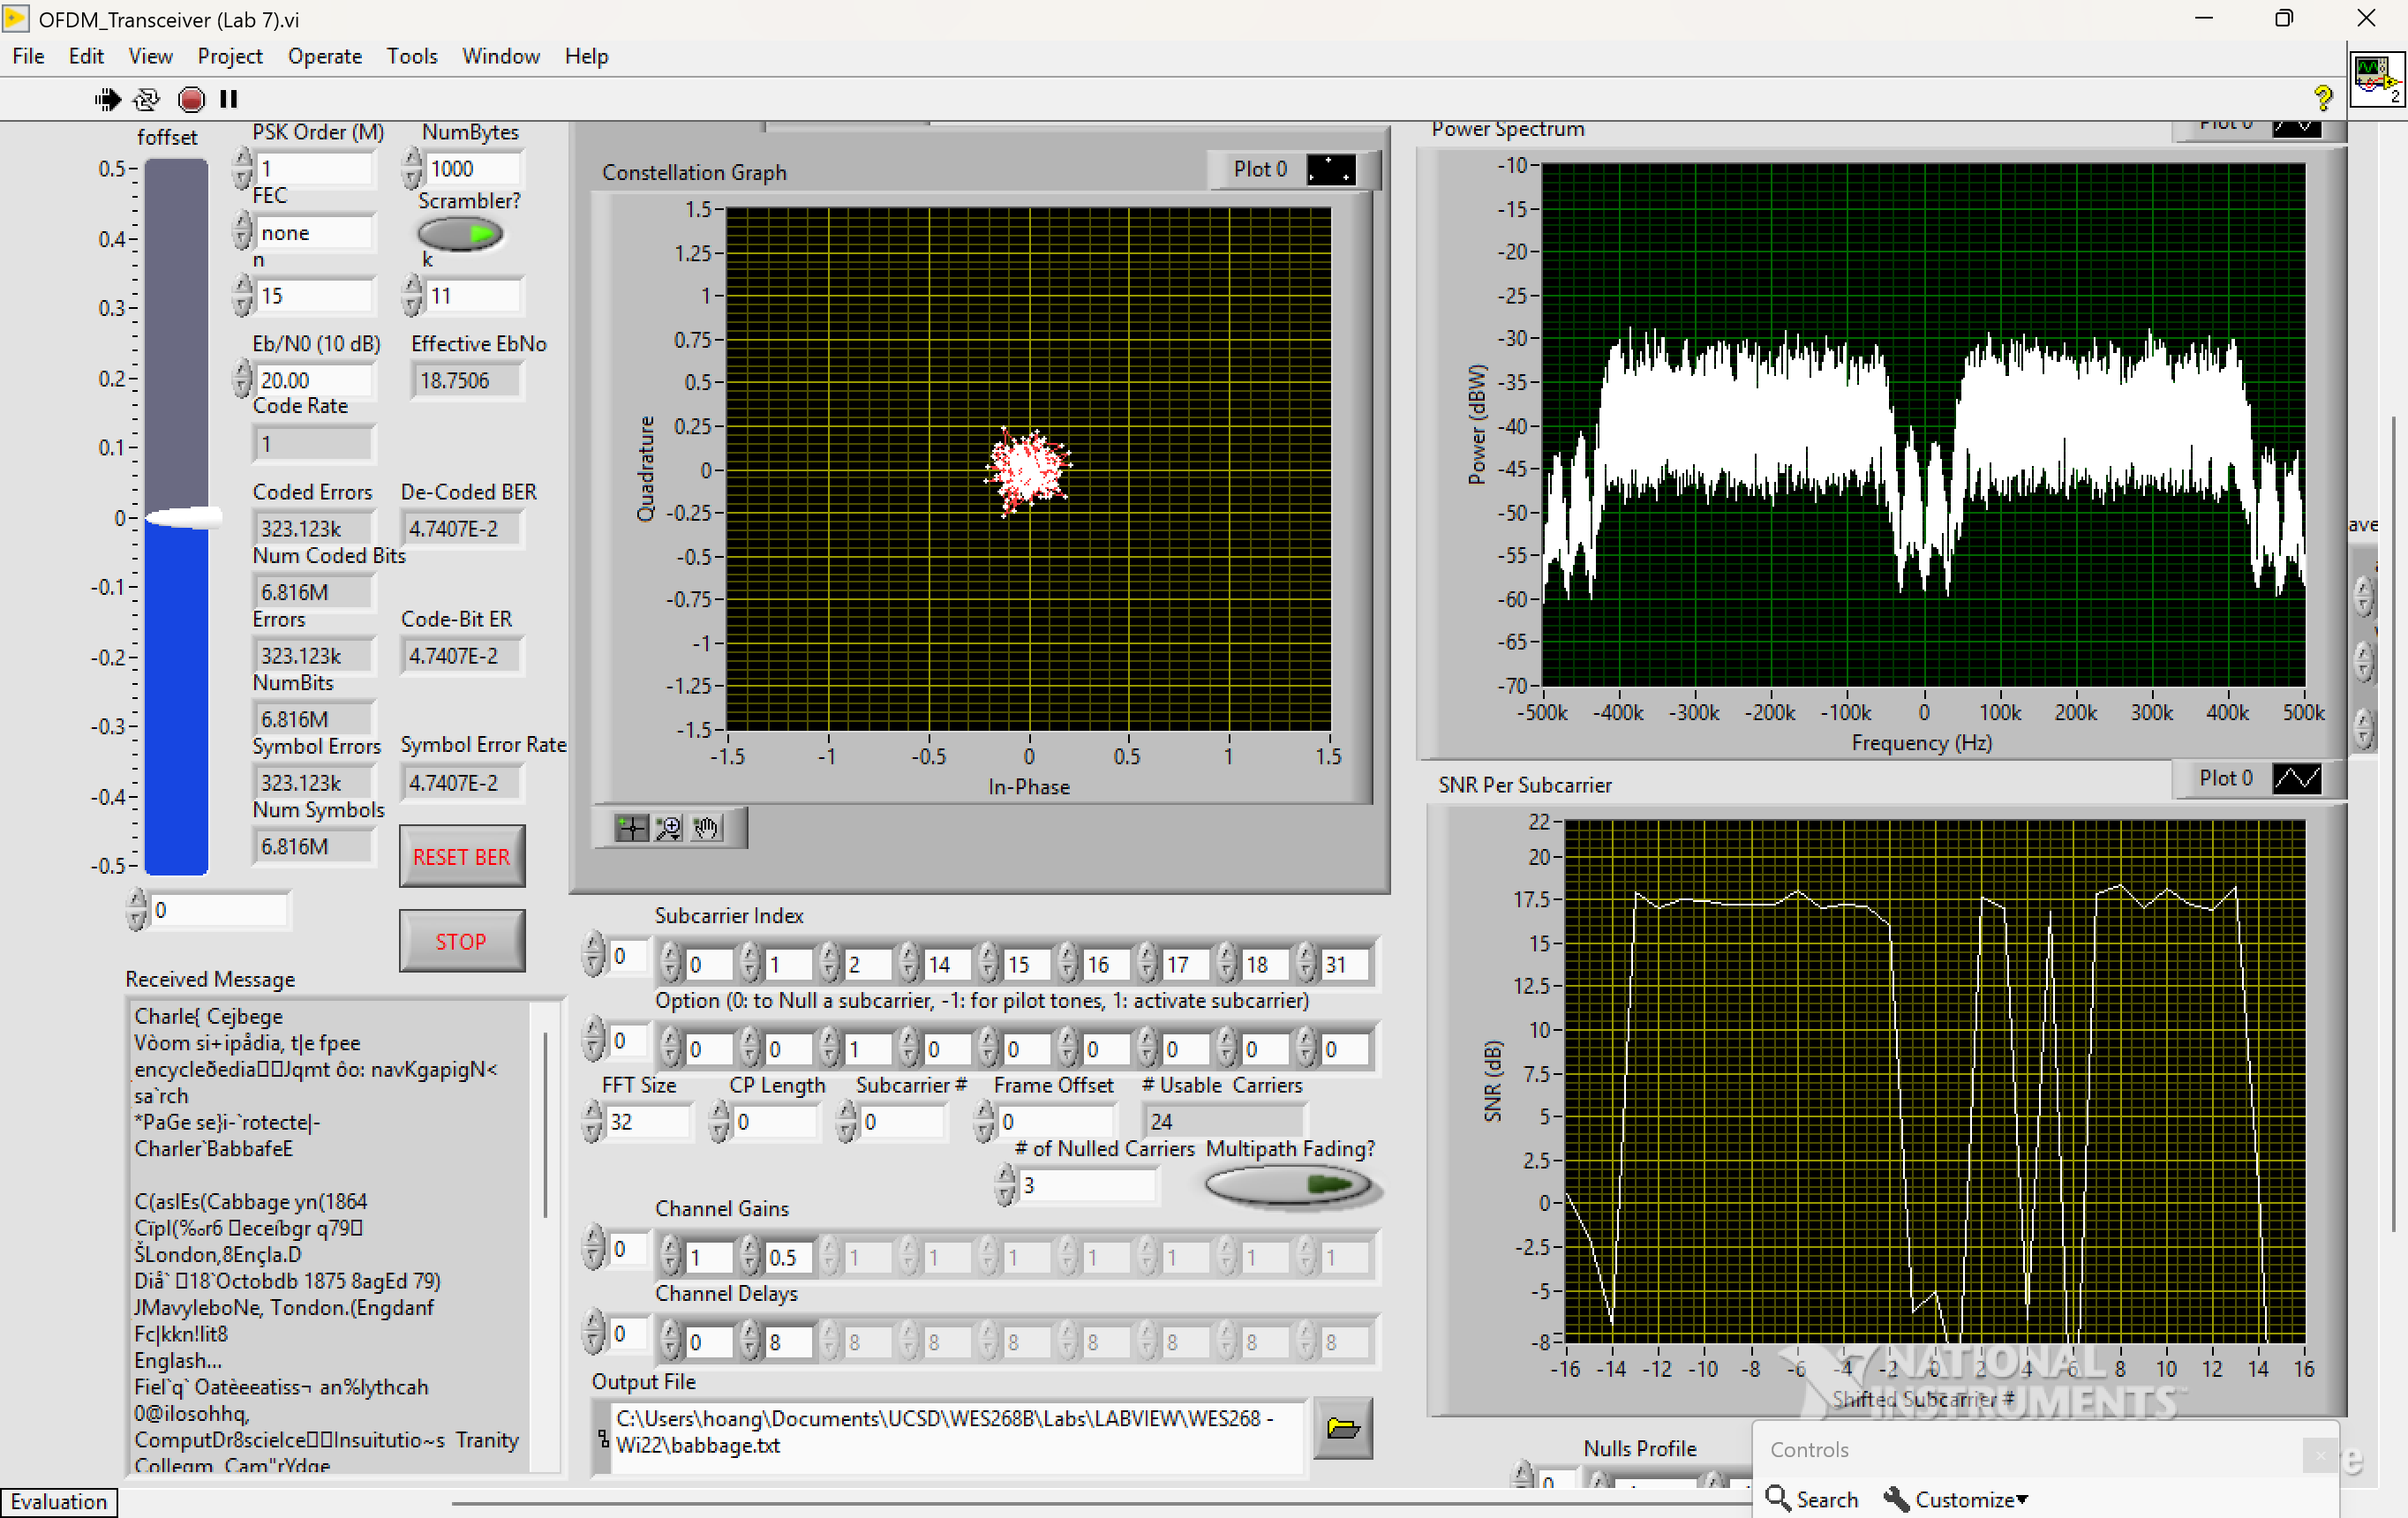
\includegraphics[width=0.7\textwidth]{lab_ss/WES268B_Lab7_Part1-1-2_FEC-None_nullCarriers-3.png}
    \caption{Lab 7 - 3 Nulled Subcarriers}
    %\label{f3}
\end{figure}

\begin{figure}[H]
    \centering
    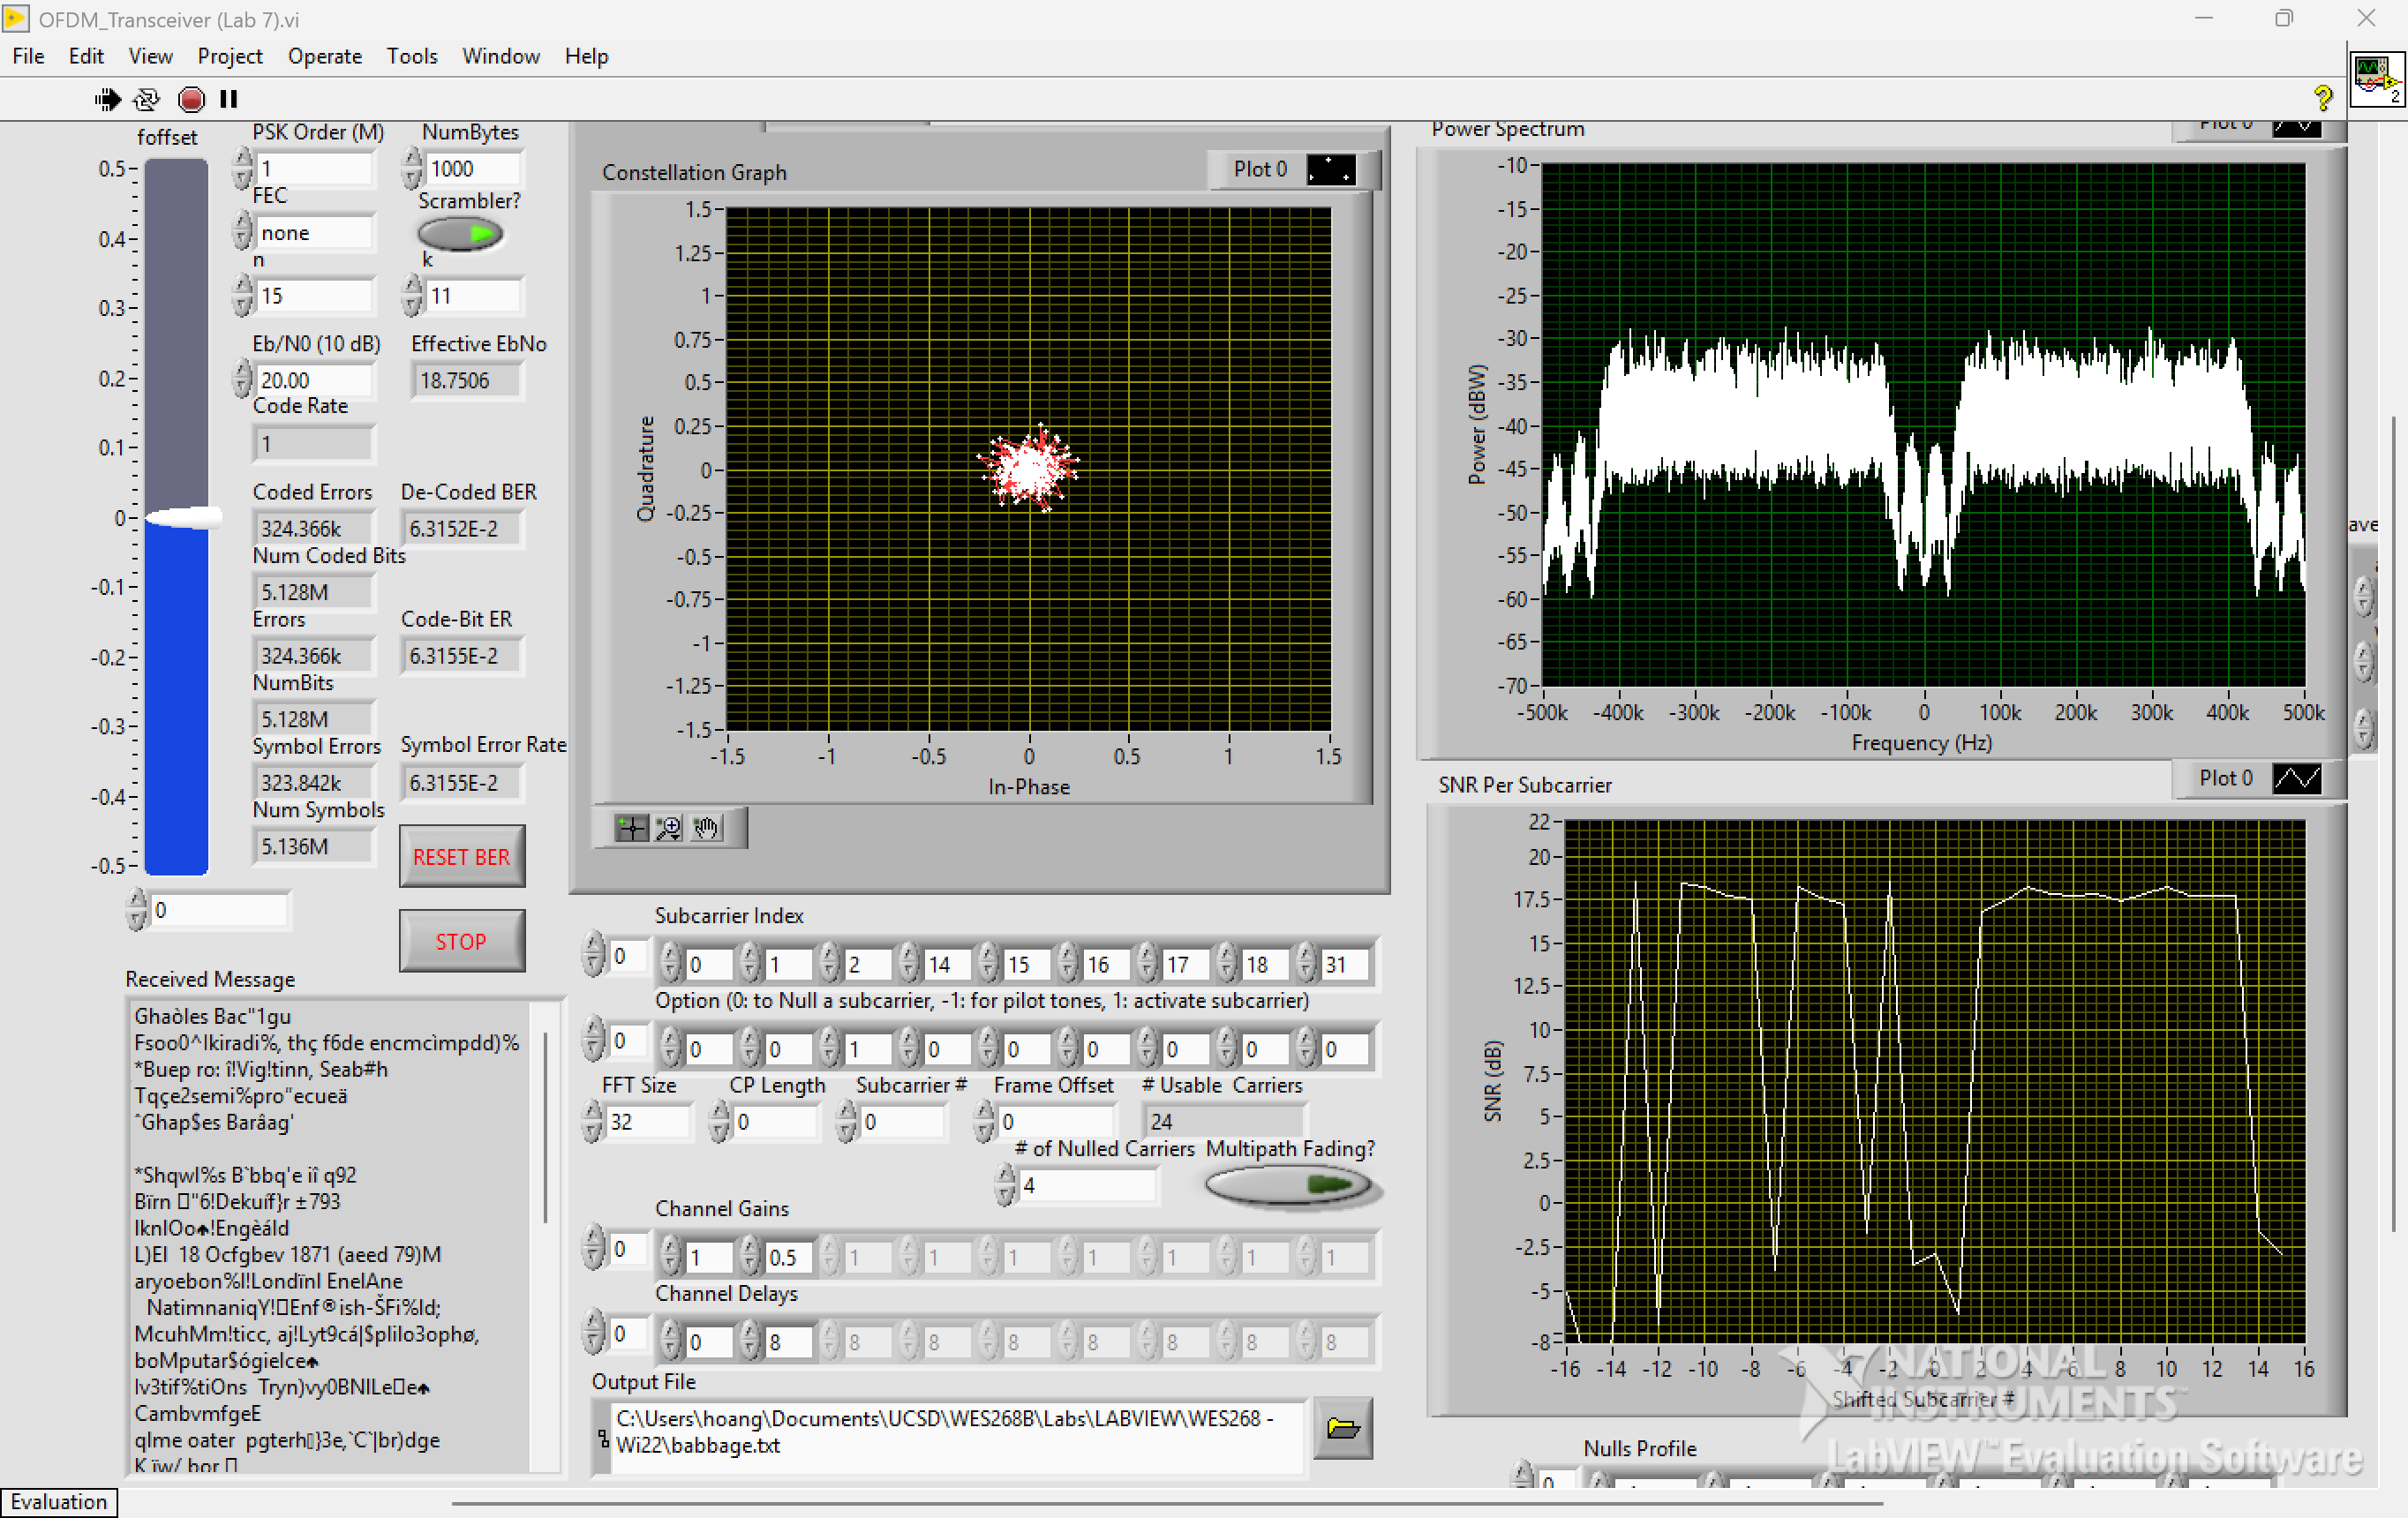
\includegraphics[width=0.7\textwidth]{lab_ss/WES268B_Lab7_Part1-1-2_FEC-None_nullCarriers-4.png}
    \caption{Lab 7 - 4 Nulled Subcarriers}
    %\label{f4}
\end{figure}

\begin{figure}[H]
    \centering
    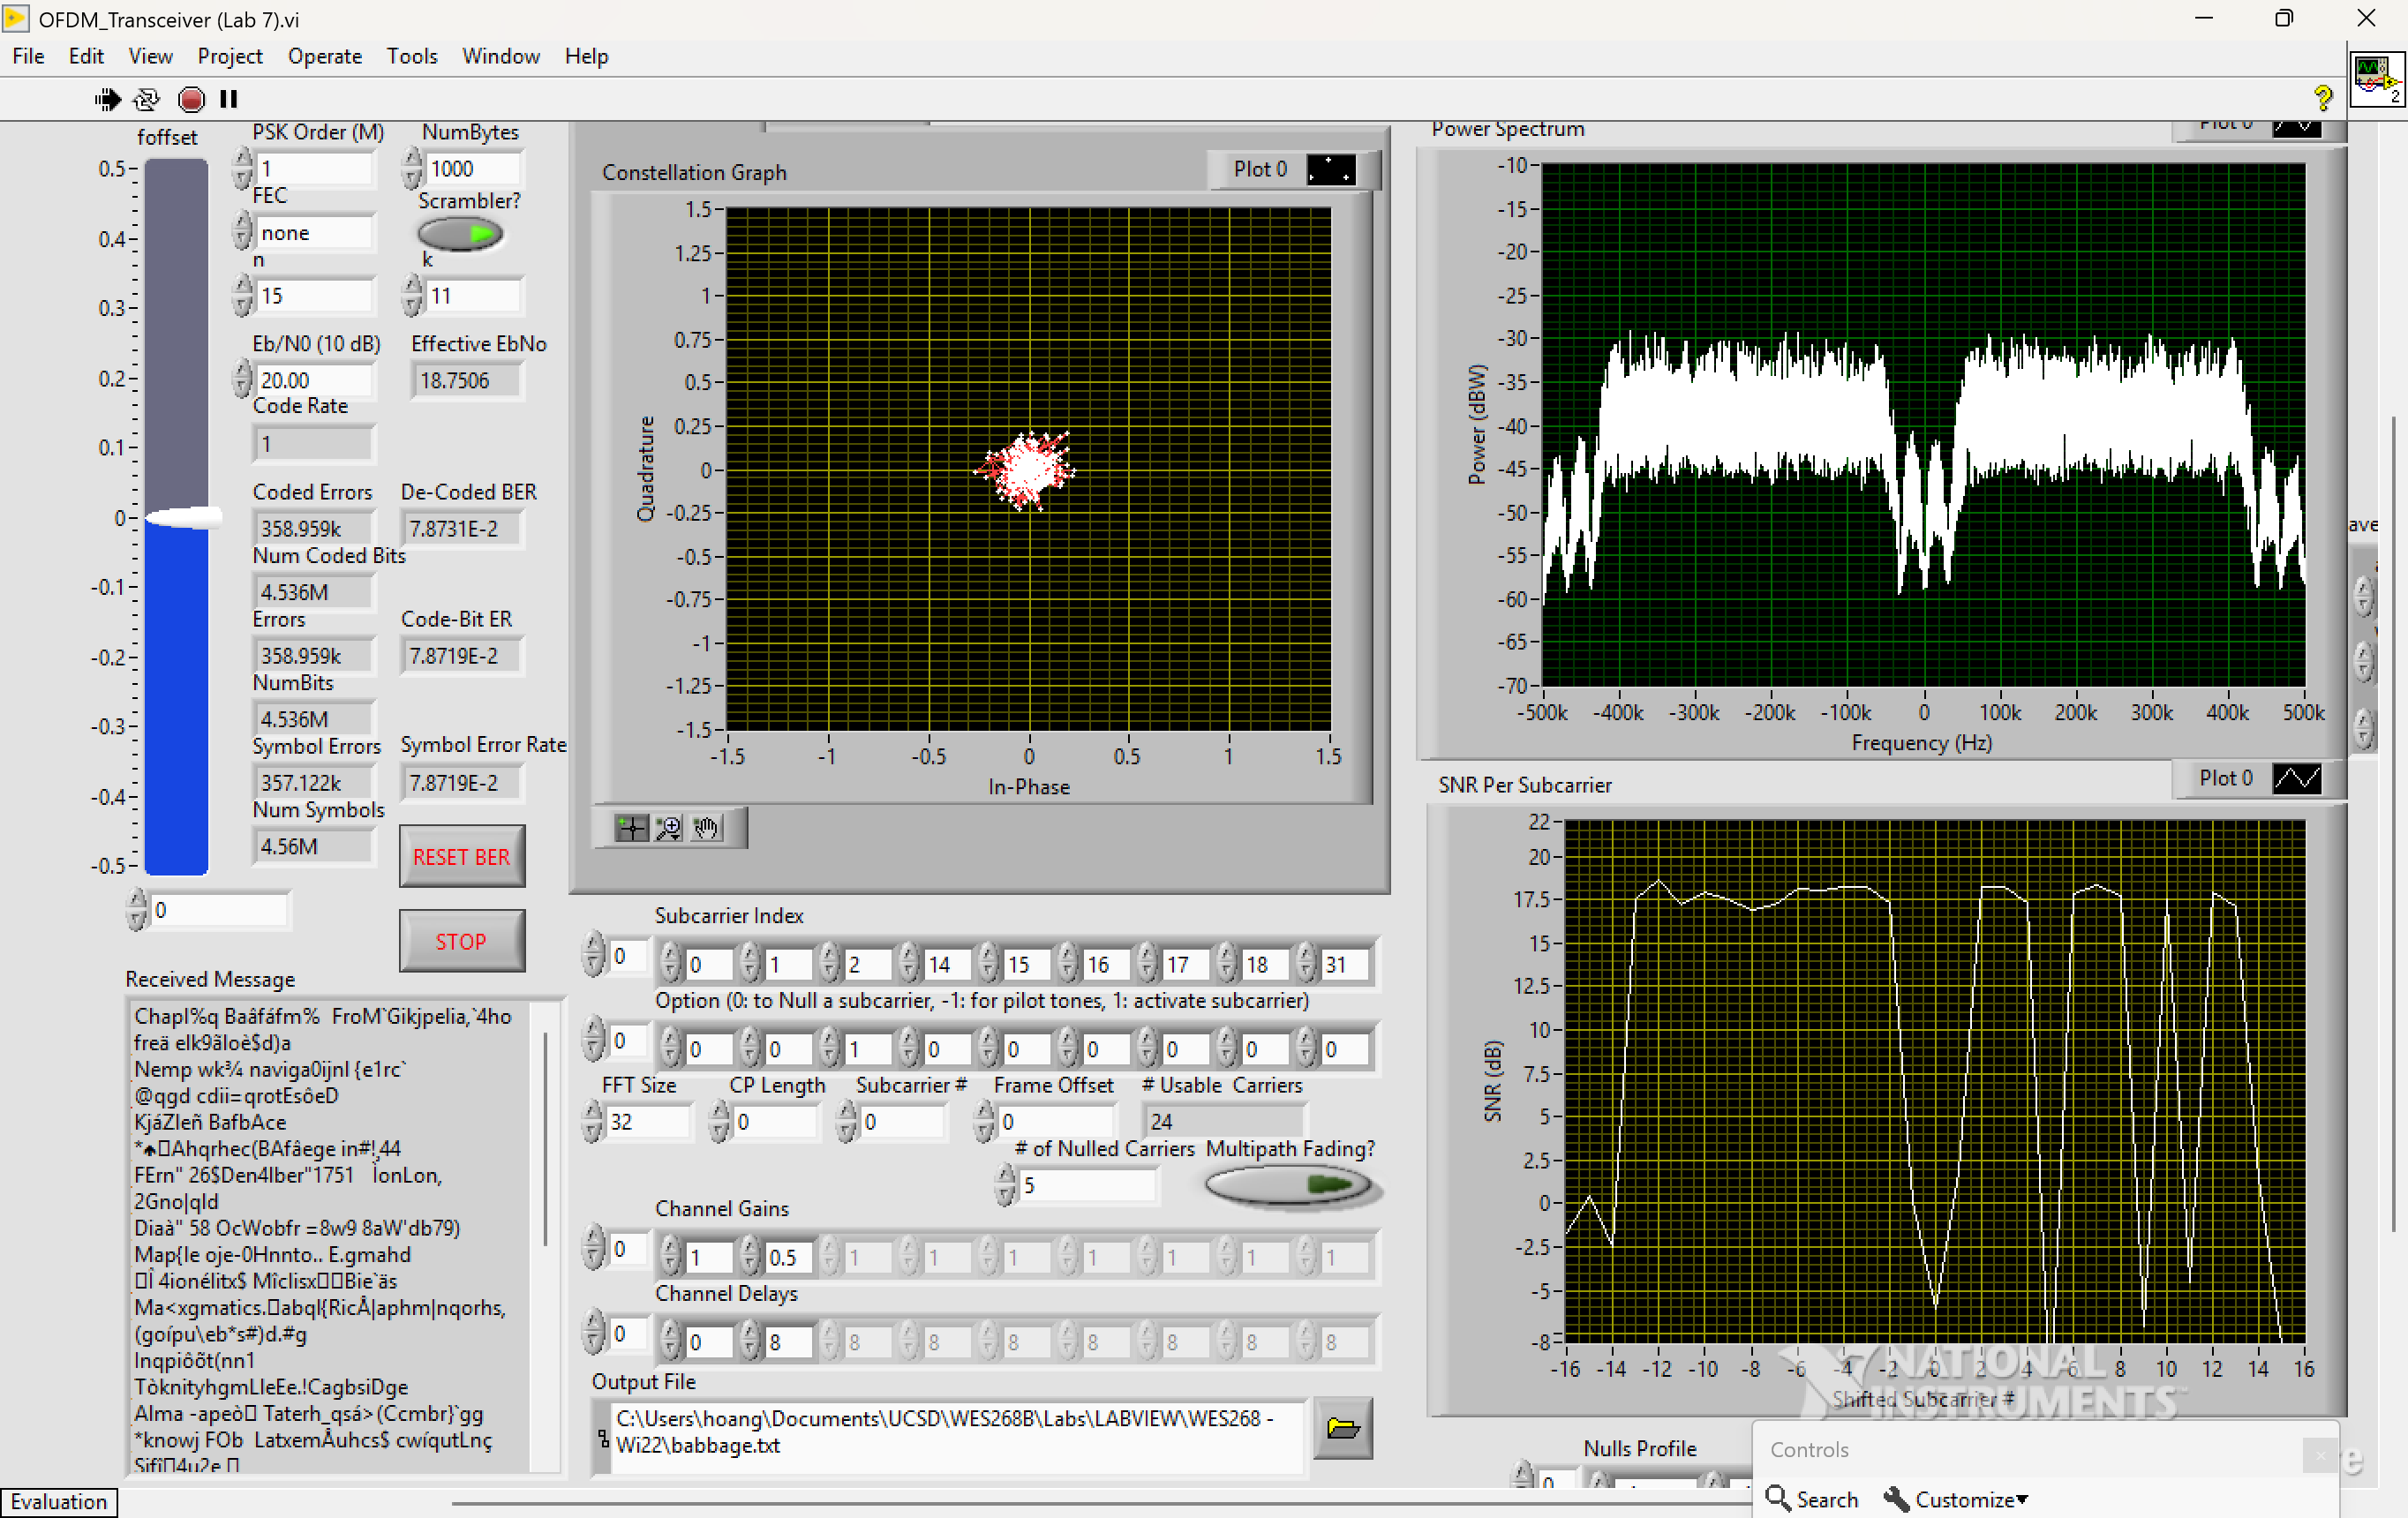
\includegraphics[width=0.7\textwidth]{lab_ss/WES268B_Lab7_Part1-1-2_FEC-None_nullCarriers-5.png}
    \caption{Lab 7 - 5 Nulled Subcarriers}
    %\label{f5}
\end{figure}

\begin{figure}[H]
    \centering
    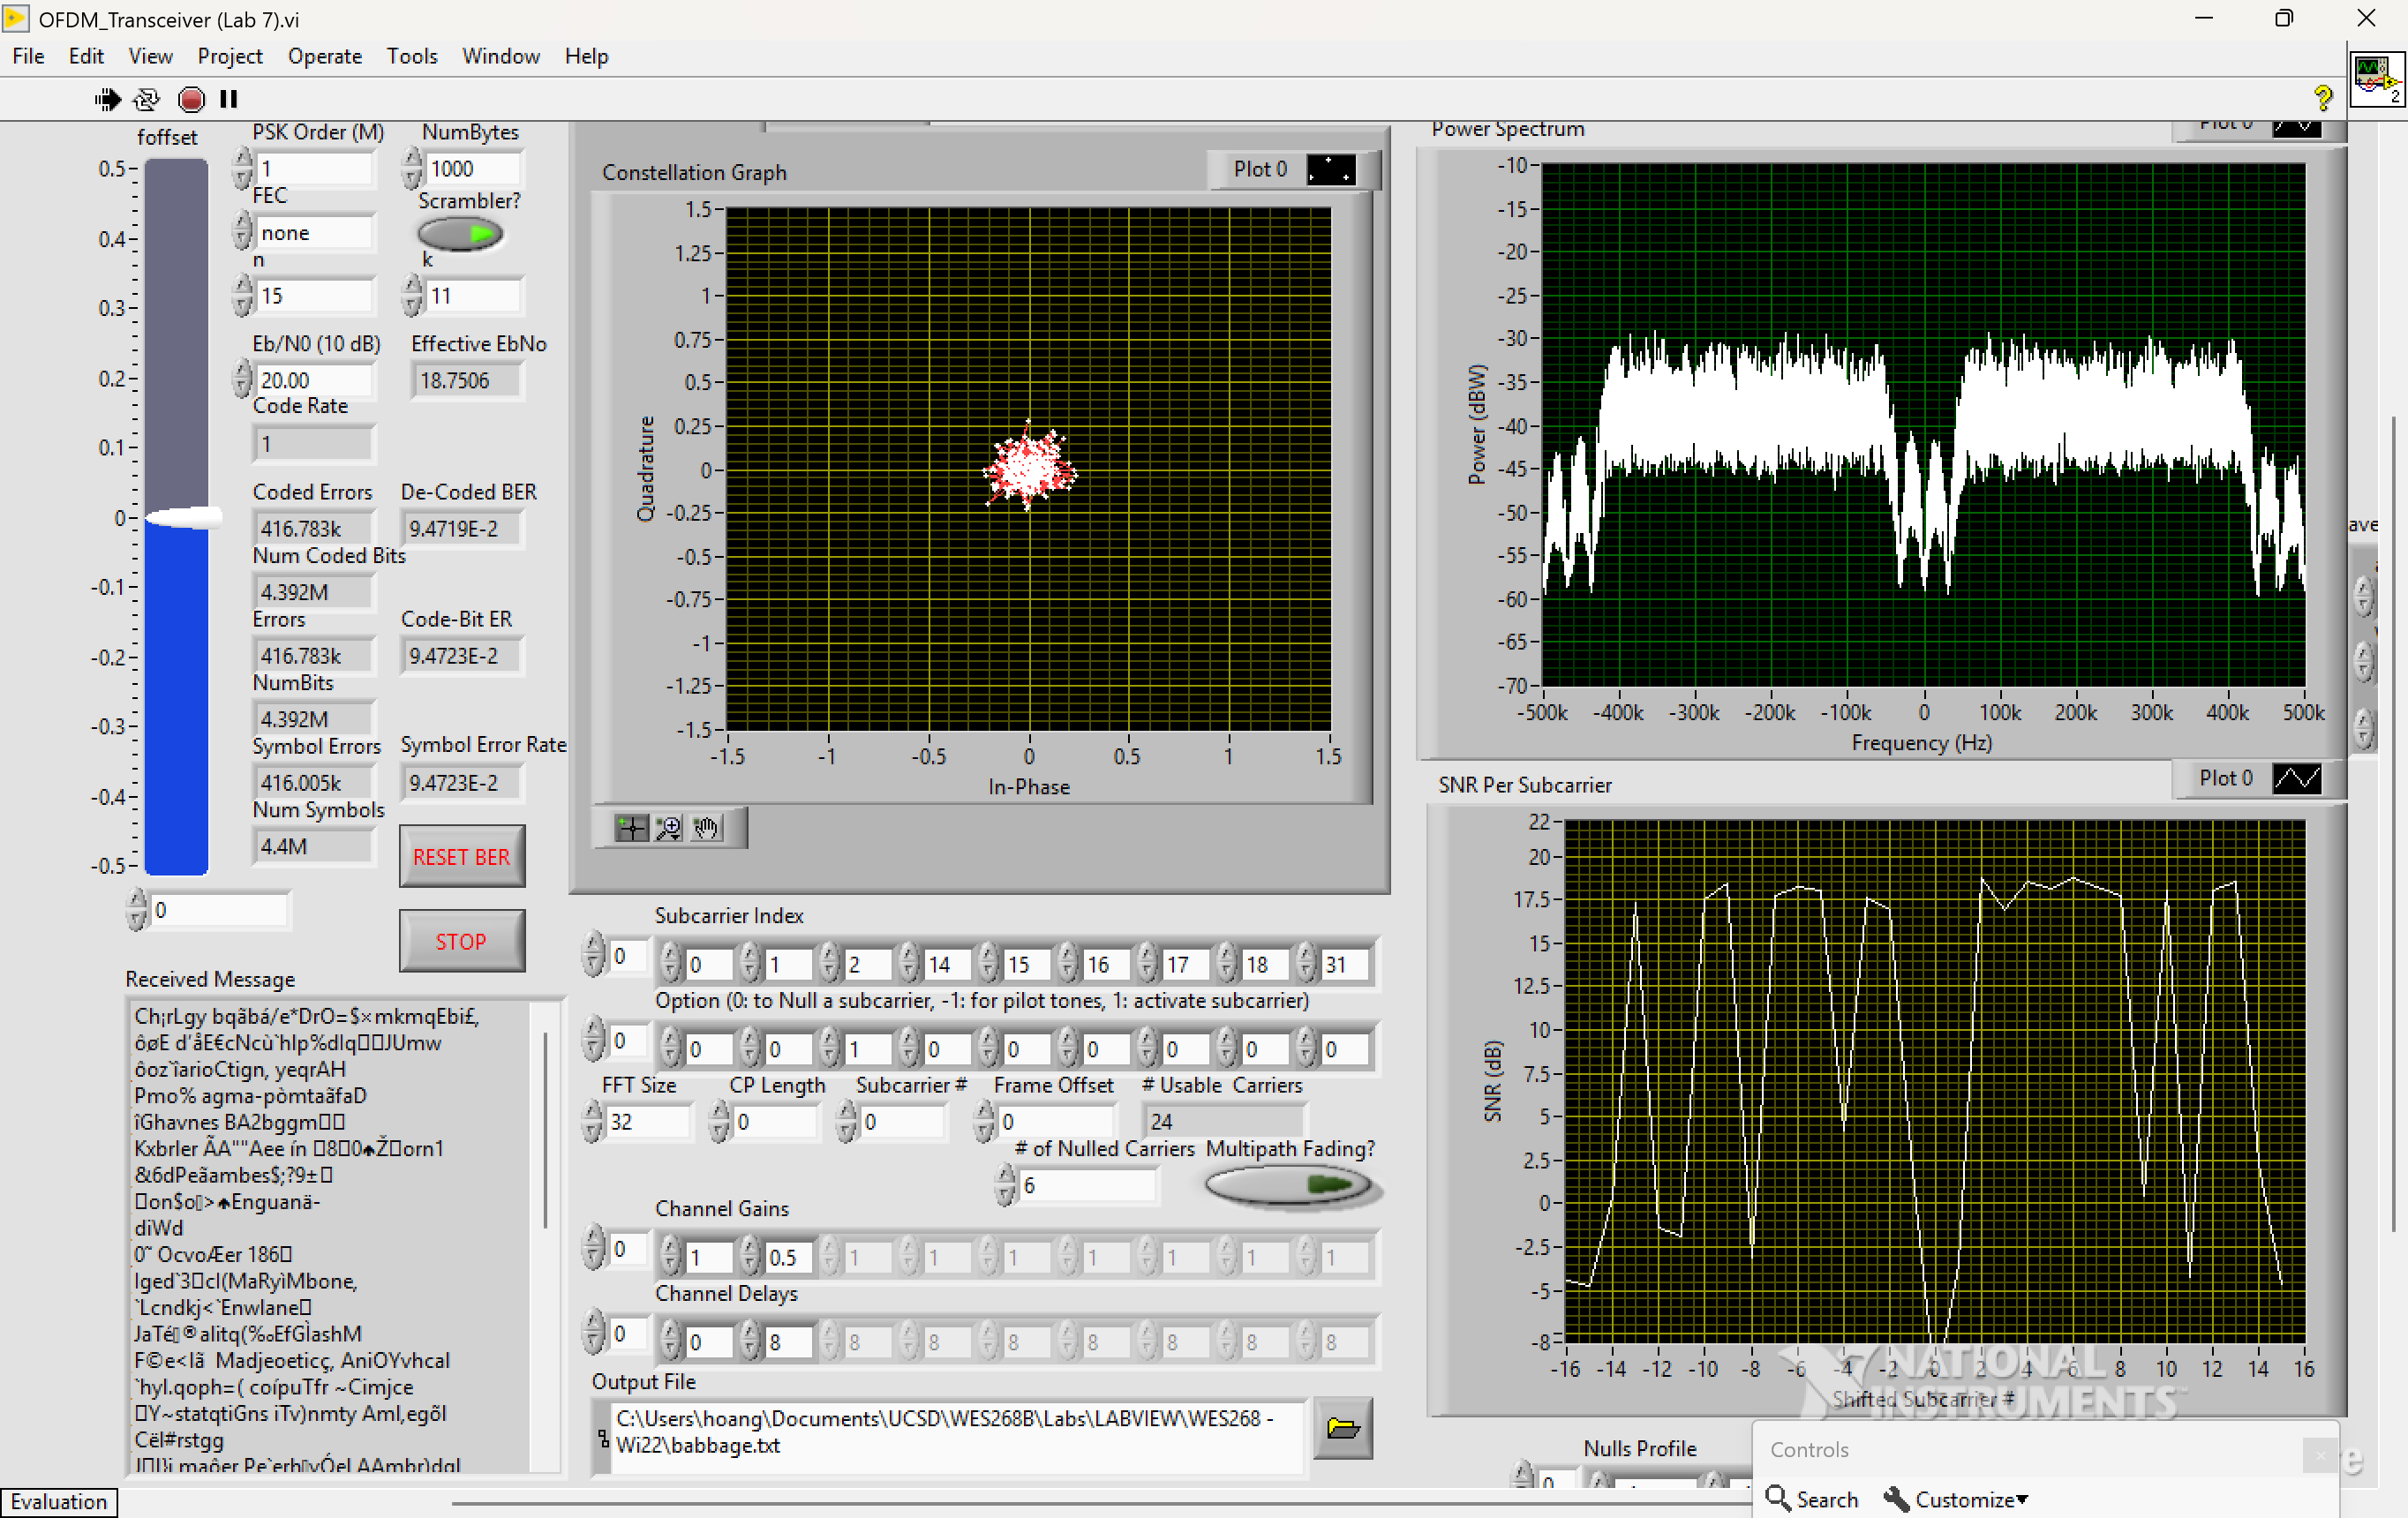
\includegraphics[width=0.7\textwidth]{lab_ss/WES268B_Lab7_Part1-1-2_FEC-None_nullCarriers-6.png}
    \caption{Lab 7 - 6 Nulled Subcarriers}
    %\label{f6}
\end{figure}

% 1.1.3
\subsubsection{ }
\begin{figure}[H]
    \centering
    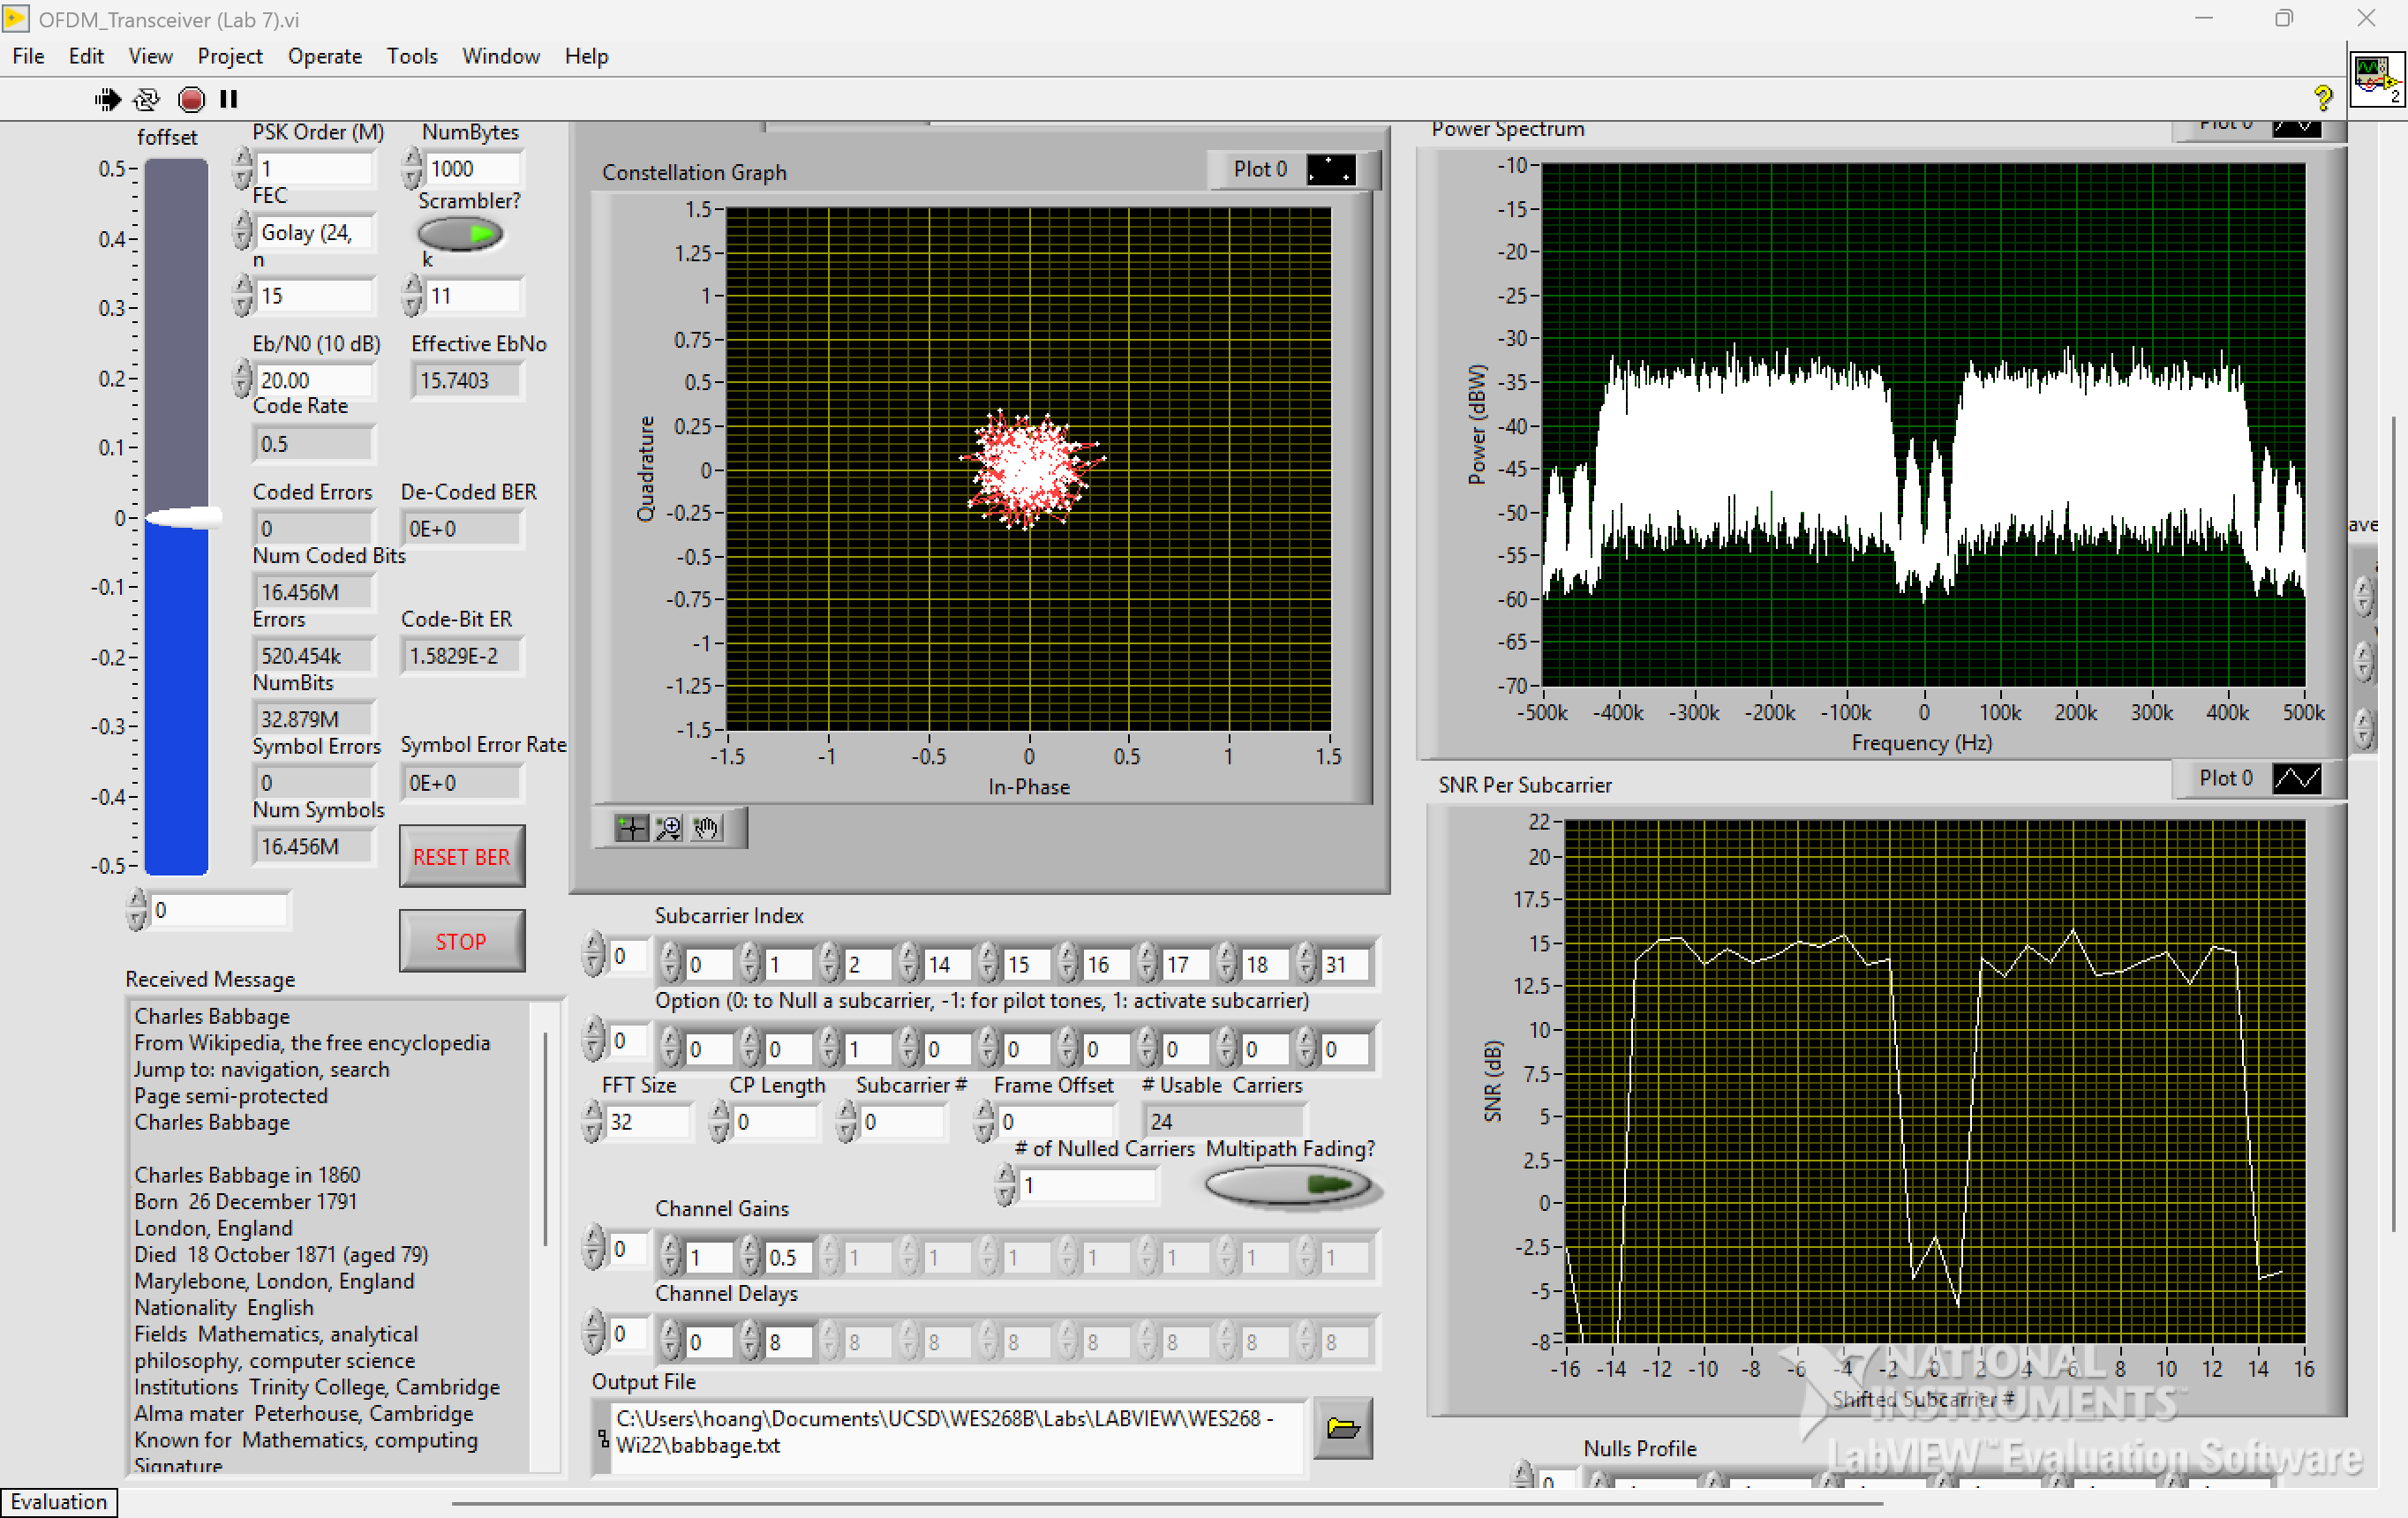
\includegraphics[width=0.7\textwidth]{lab_ss/WES268B_Lab7_Part1-1-3_FEC-Golay24_nullCarriers-1_BER-0.png}
    \caption{Lab 7 - 1 Nulled Subcarrier Golay (24,12)}
    %\label{f7}
\end{figure}

\begin{figure}[H]
    \centering
    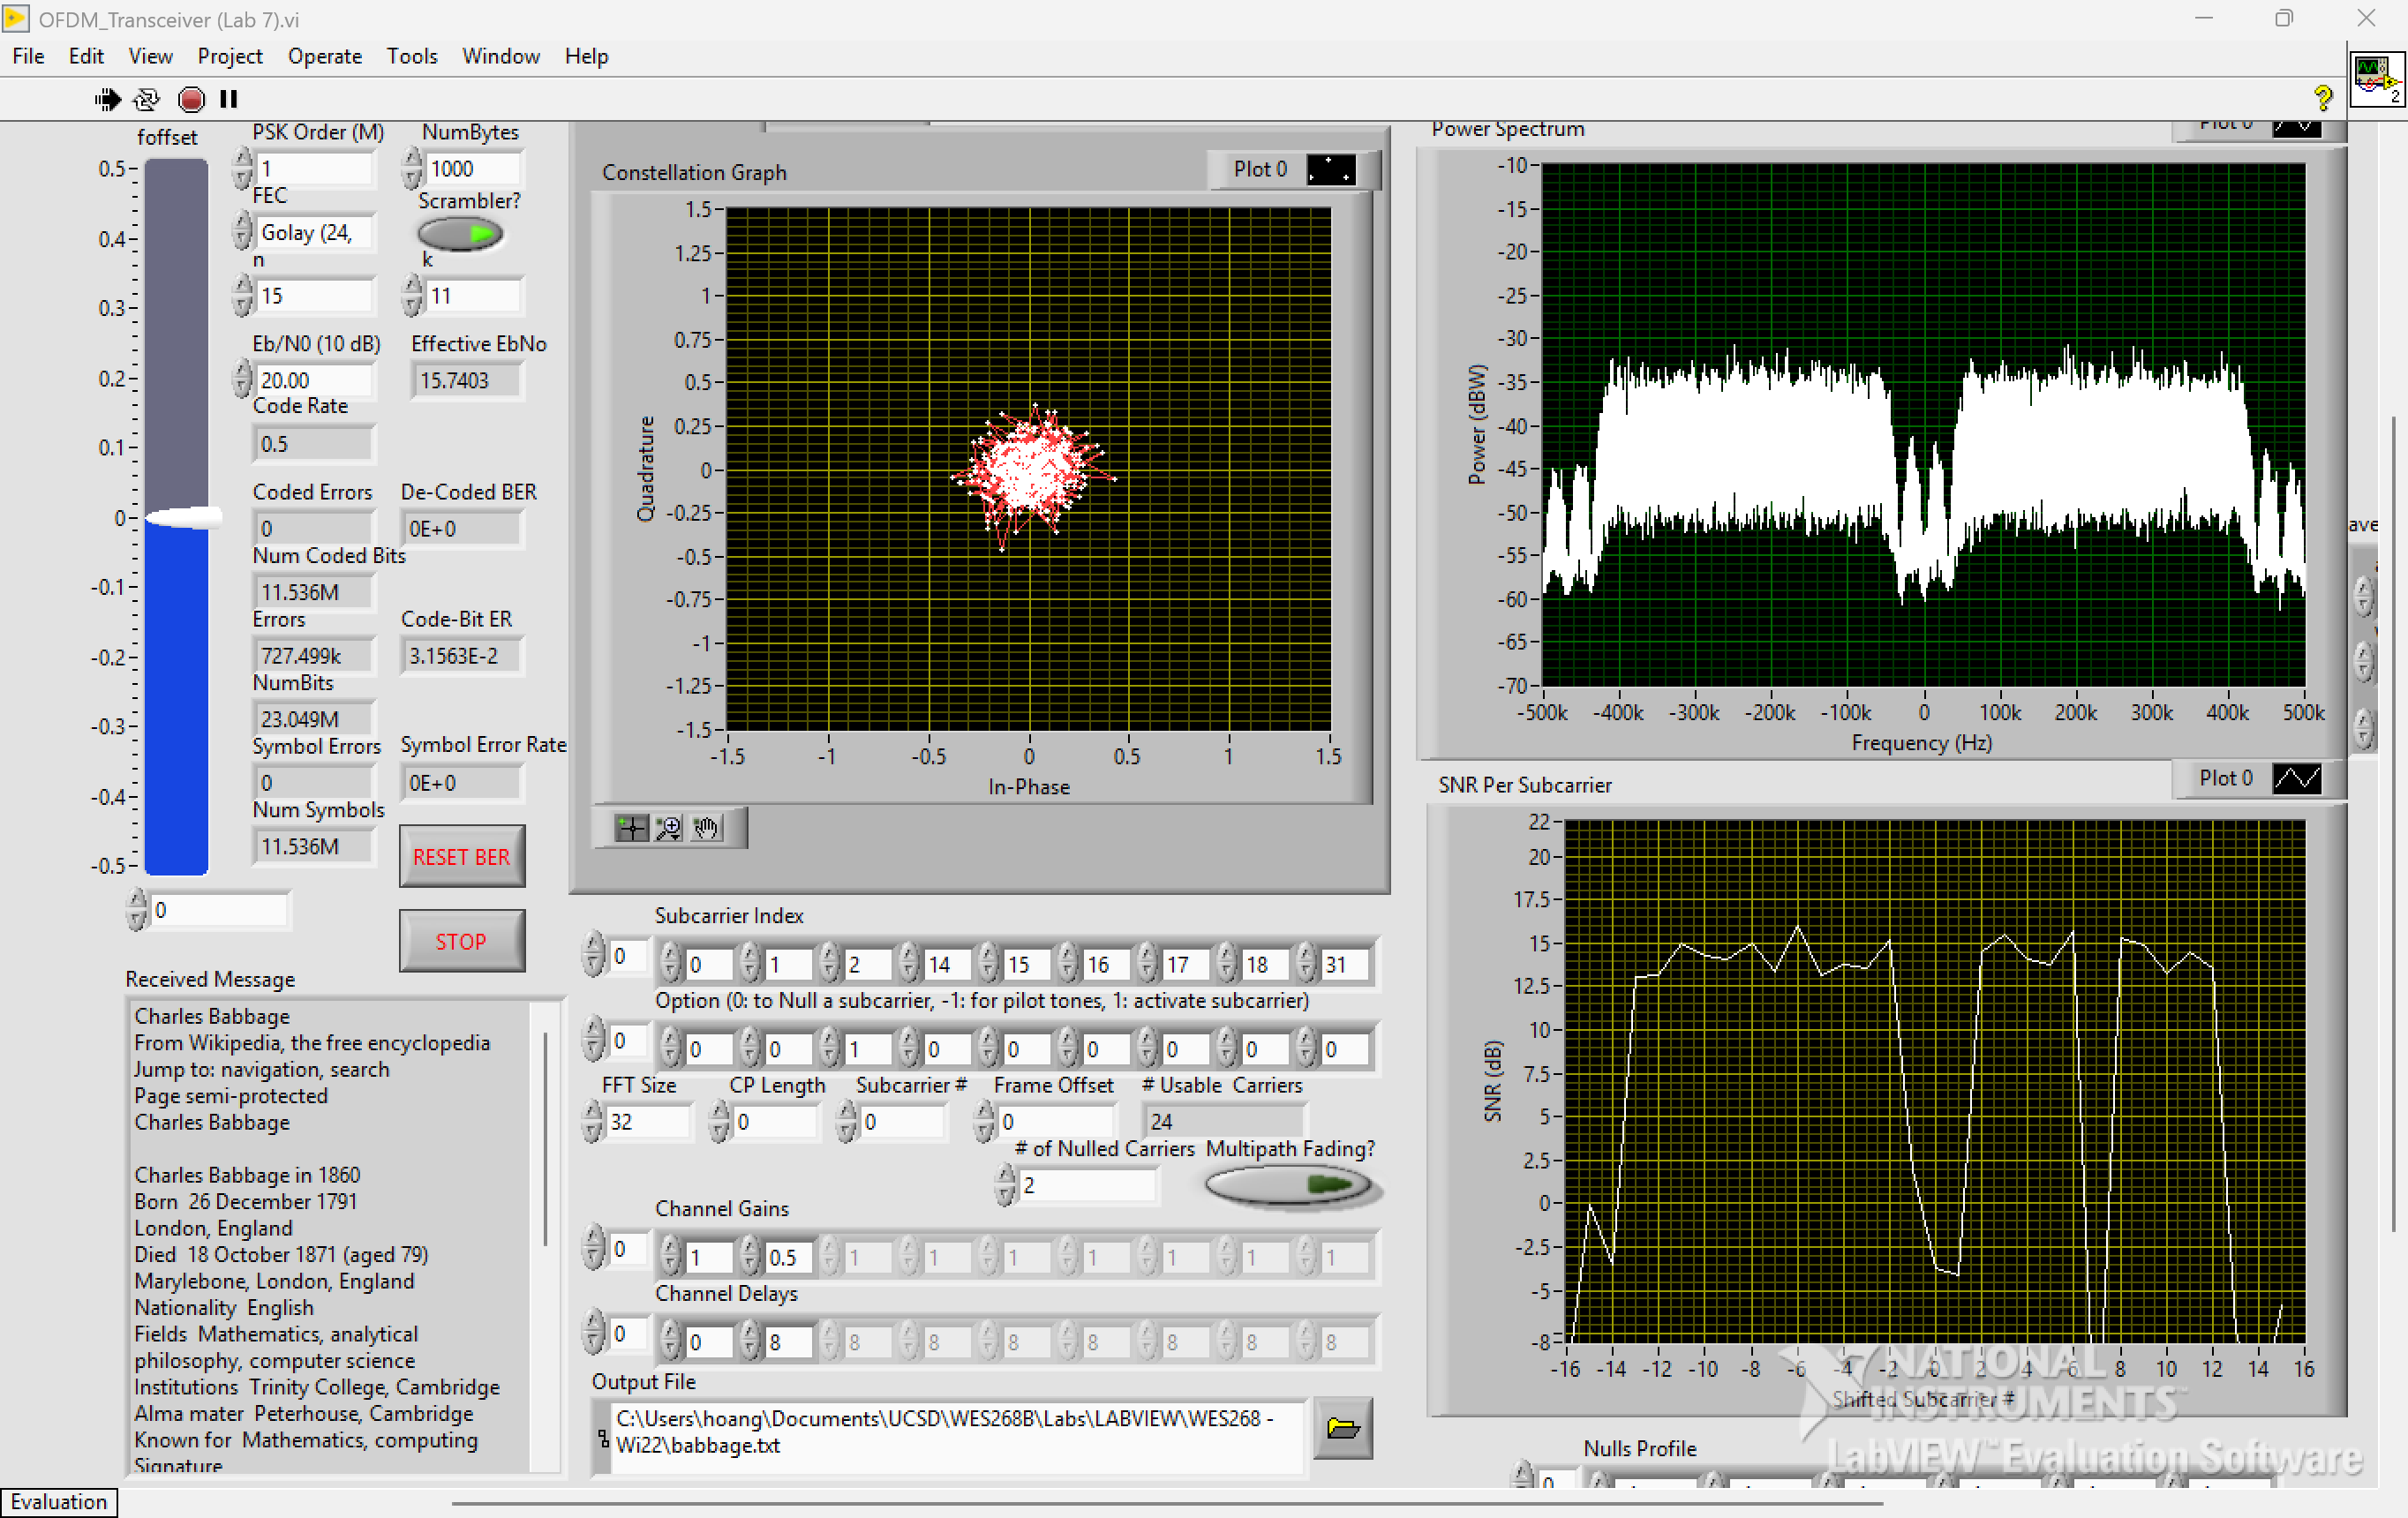
\includegraphics[width=0.7\textwidth]{lab_ss/WES268B_Lab7_Part1-1-3_FEC-Golay24_nullCarriers-2_BER-0.png}
    \caption{Lab 7 - 2 Nulled Subcarriers Golay (24,12)}
    %\label{f8}
\end{figure}

\begin{figure}[H]
    \centering
    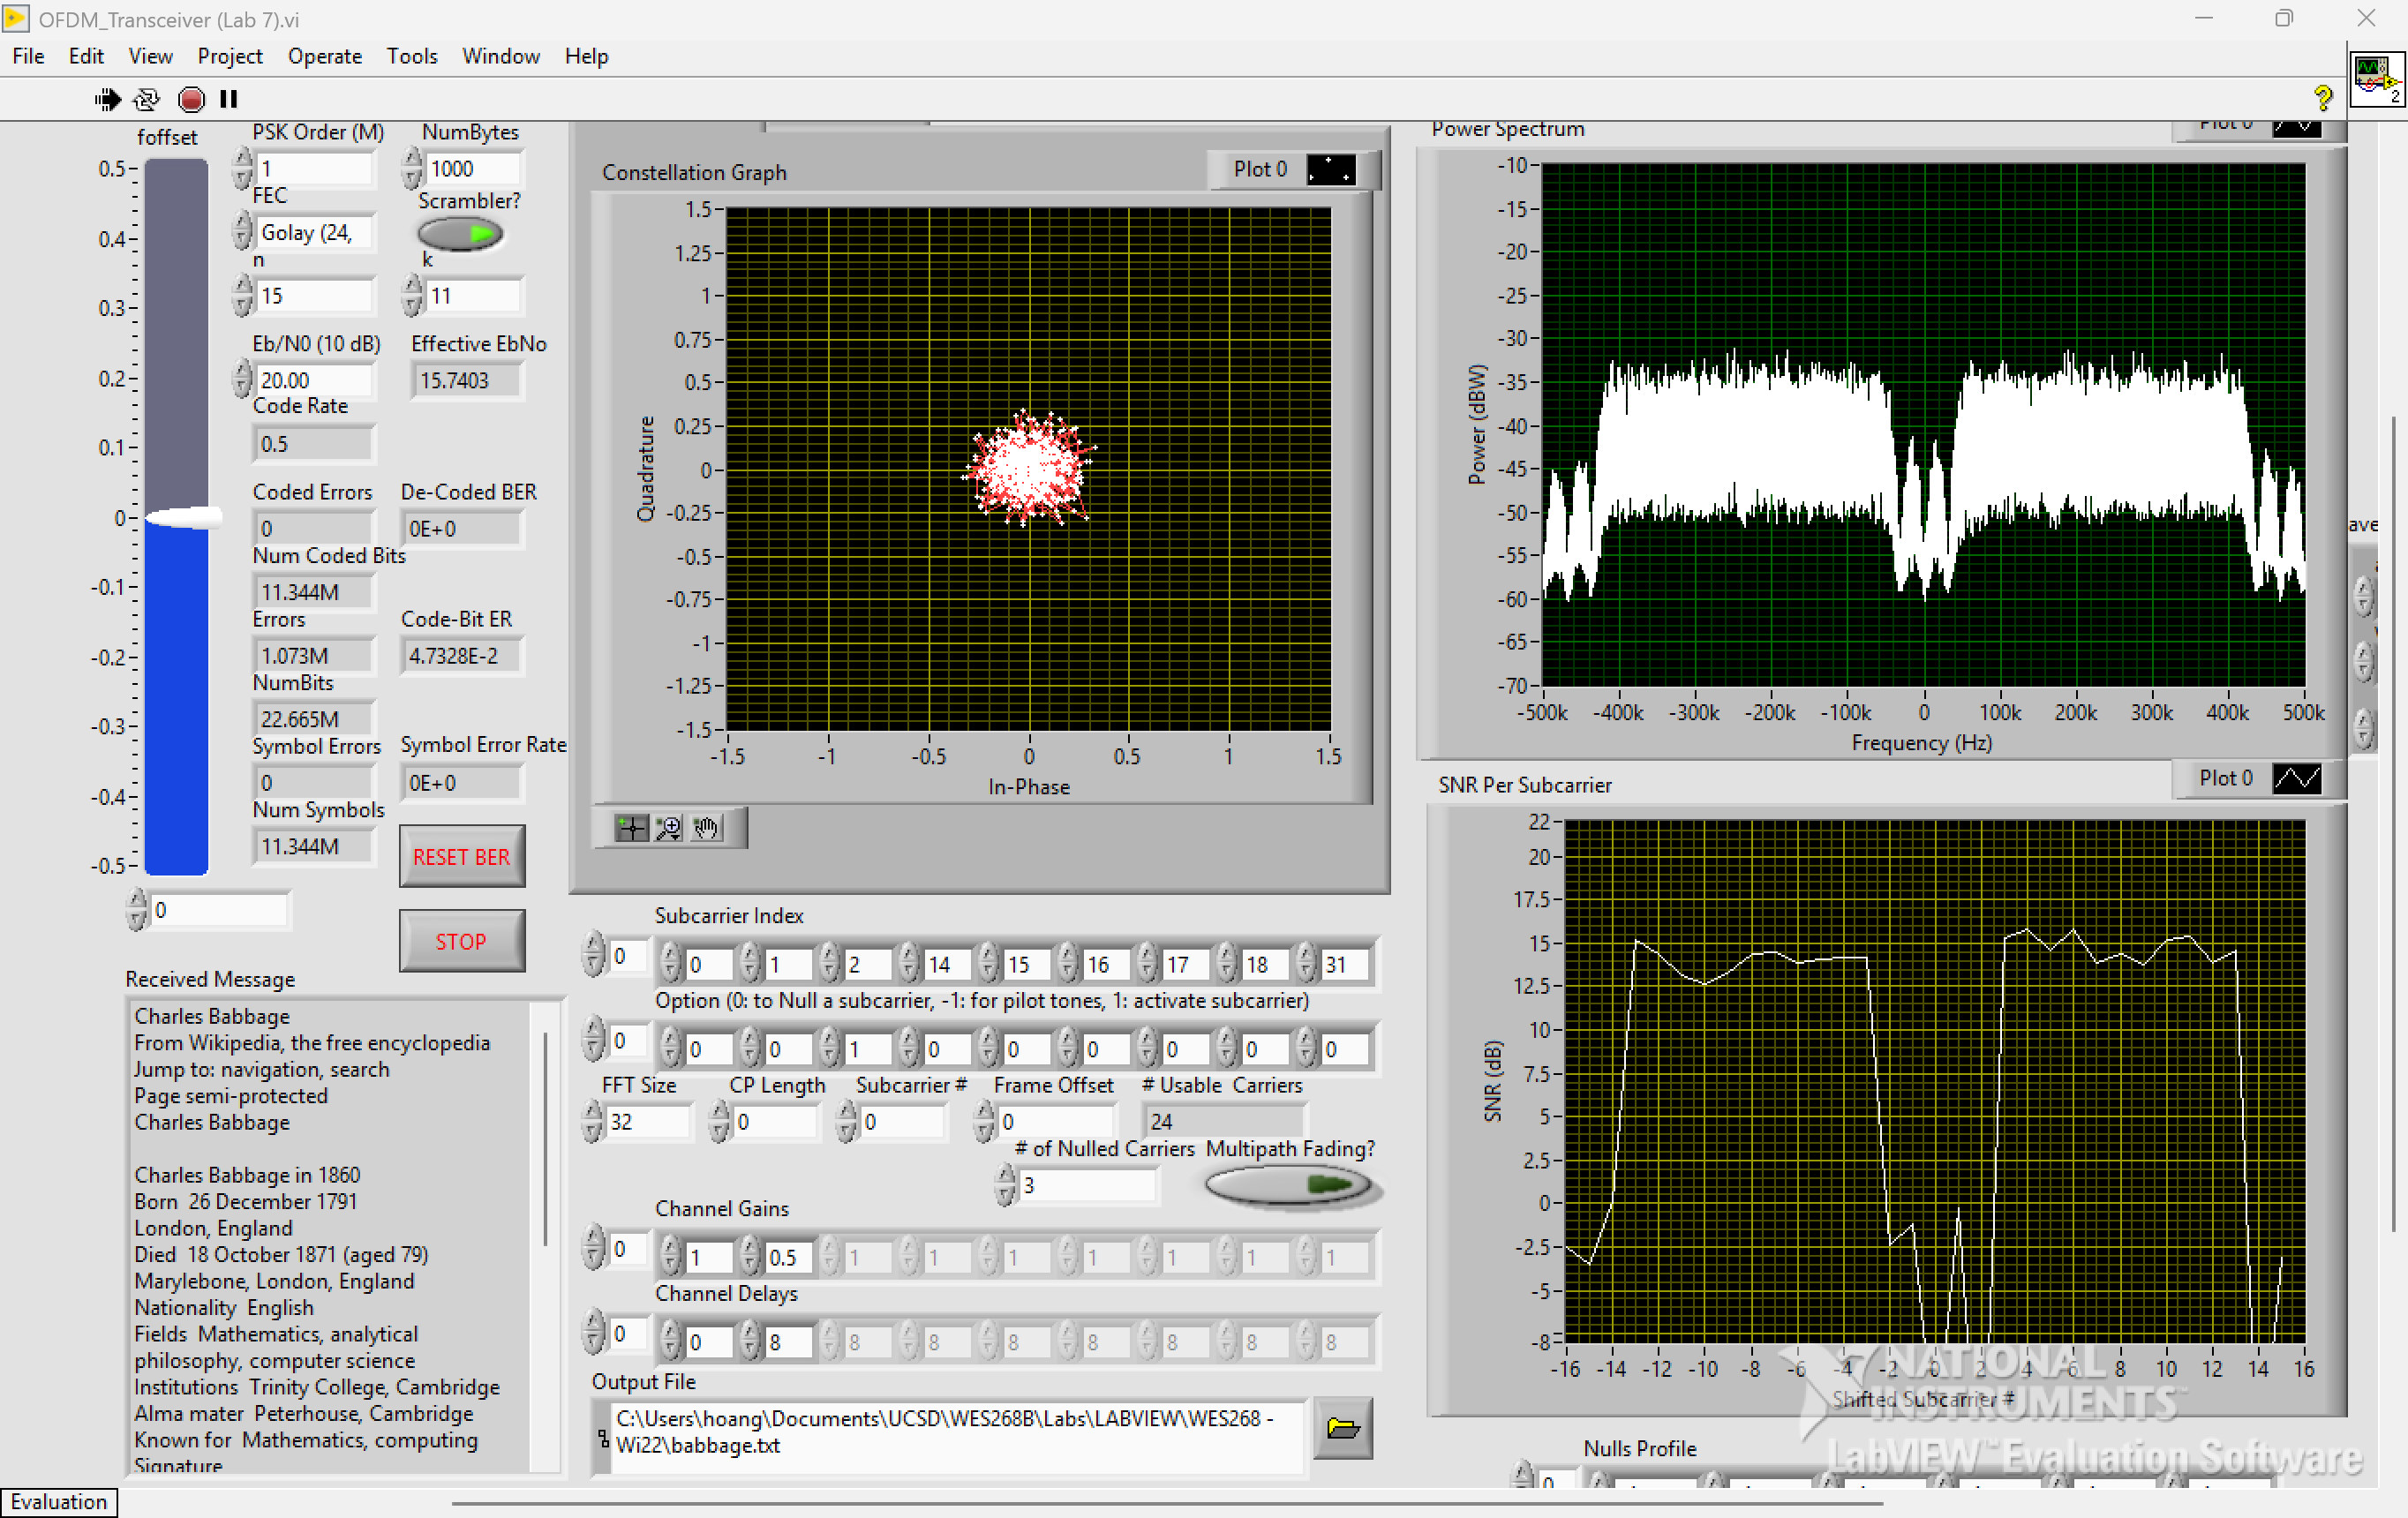
\includegraphics[width=0.7\textwidth]{lab_ss/WES268B_Lab7_Part1-1-3_FEC-Golay24_nullCarriers-3_BER-0.png}
    \caption{Lab 7 - 3 Nulled Subcarriers Golay (24,12)}
    %\label{f9}
\end{figure}

\begin{figure}[H]
    \centering
    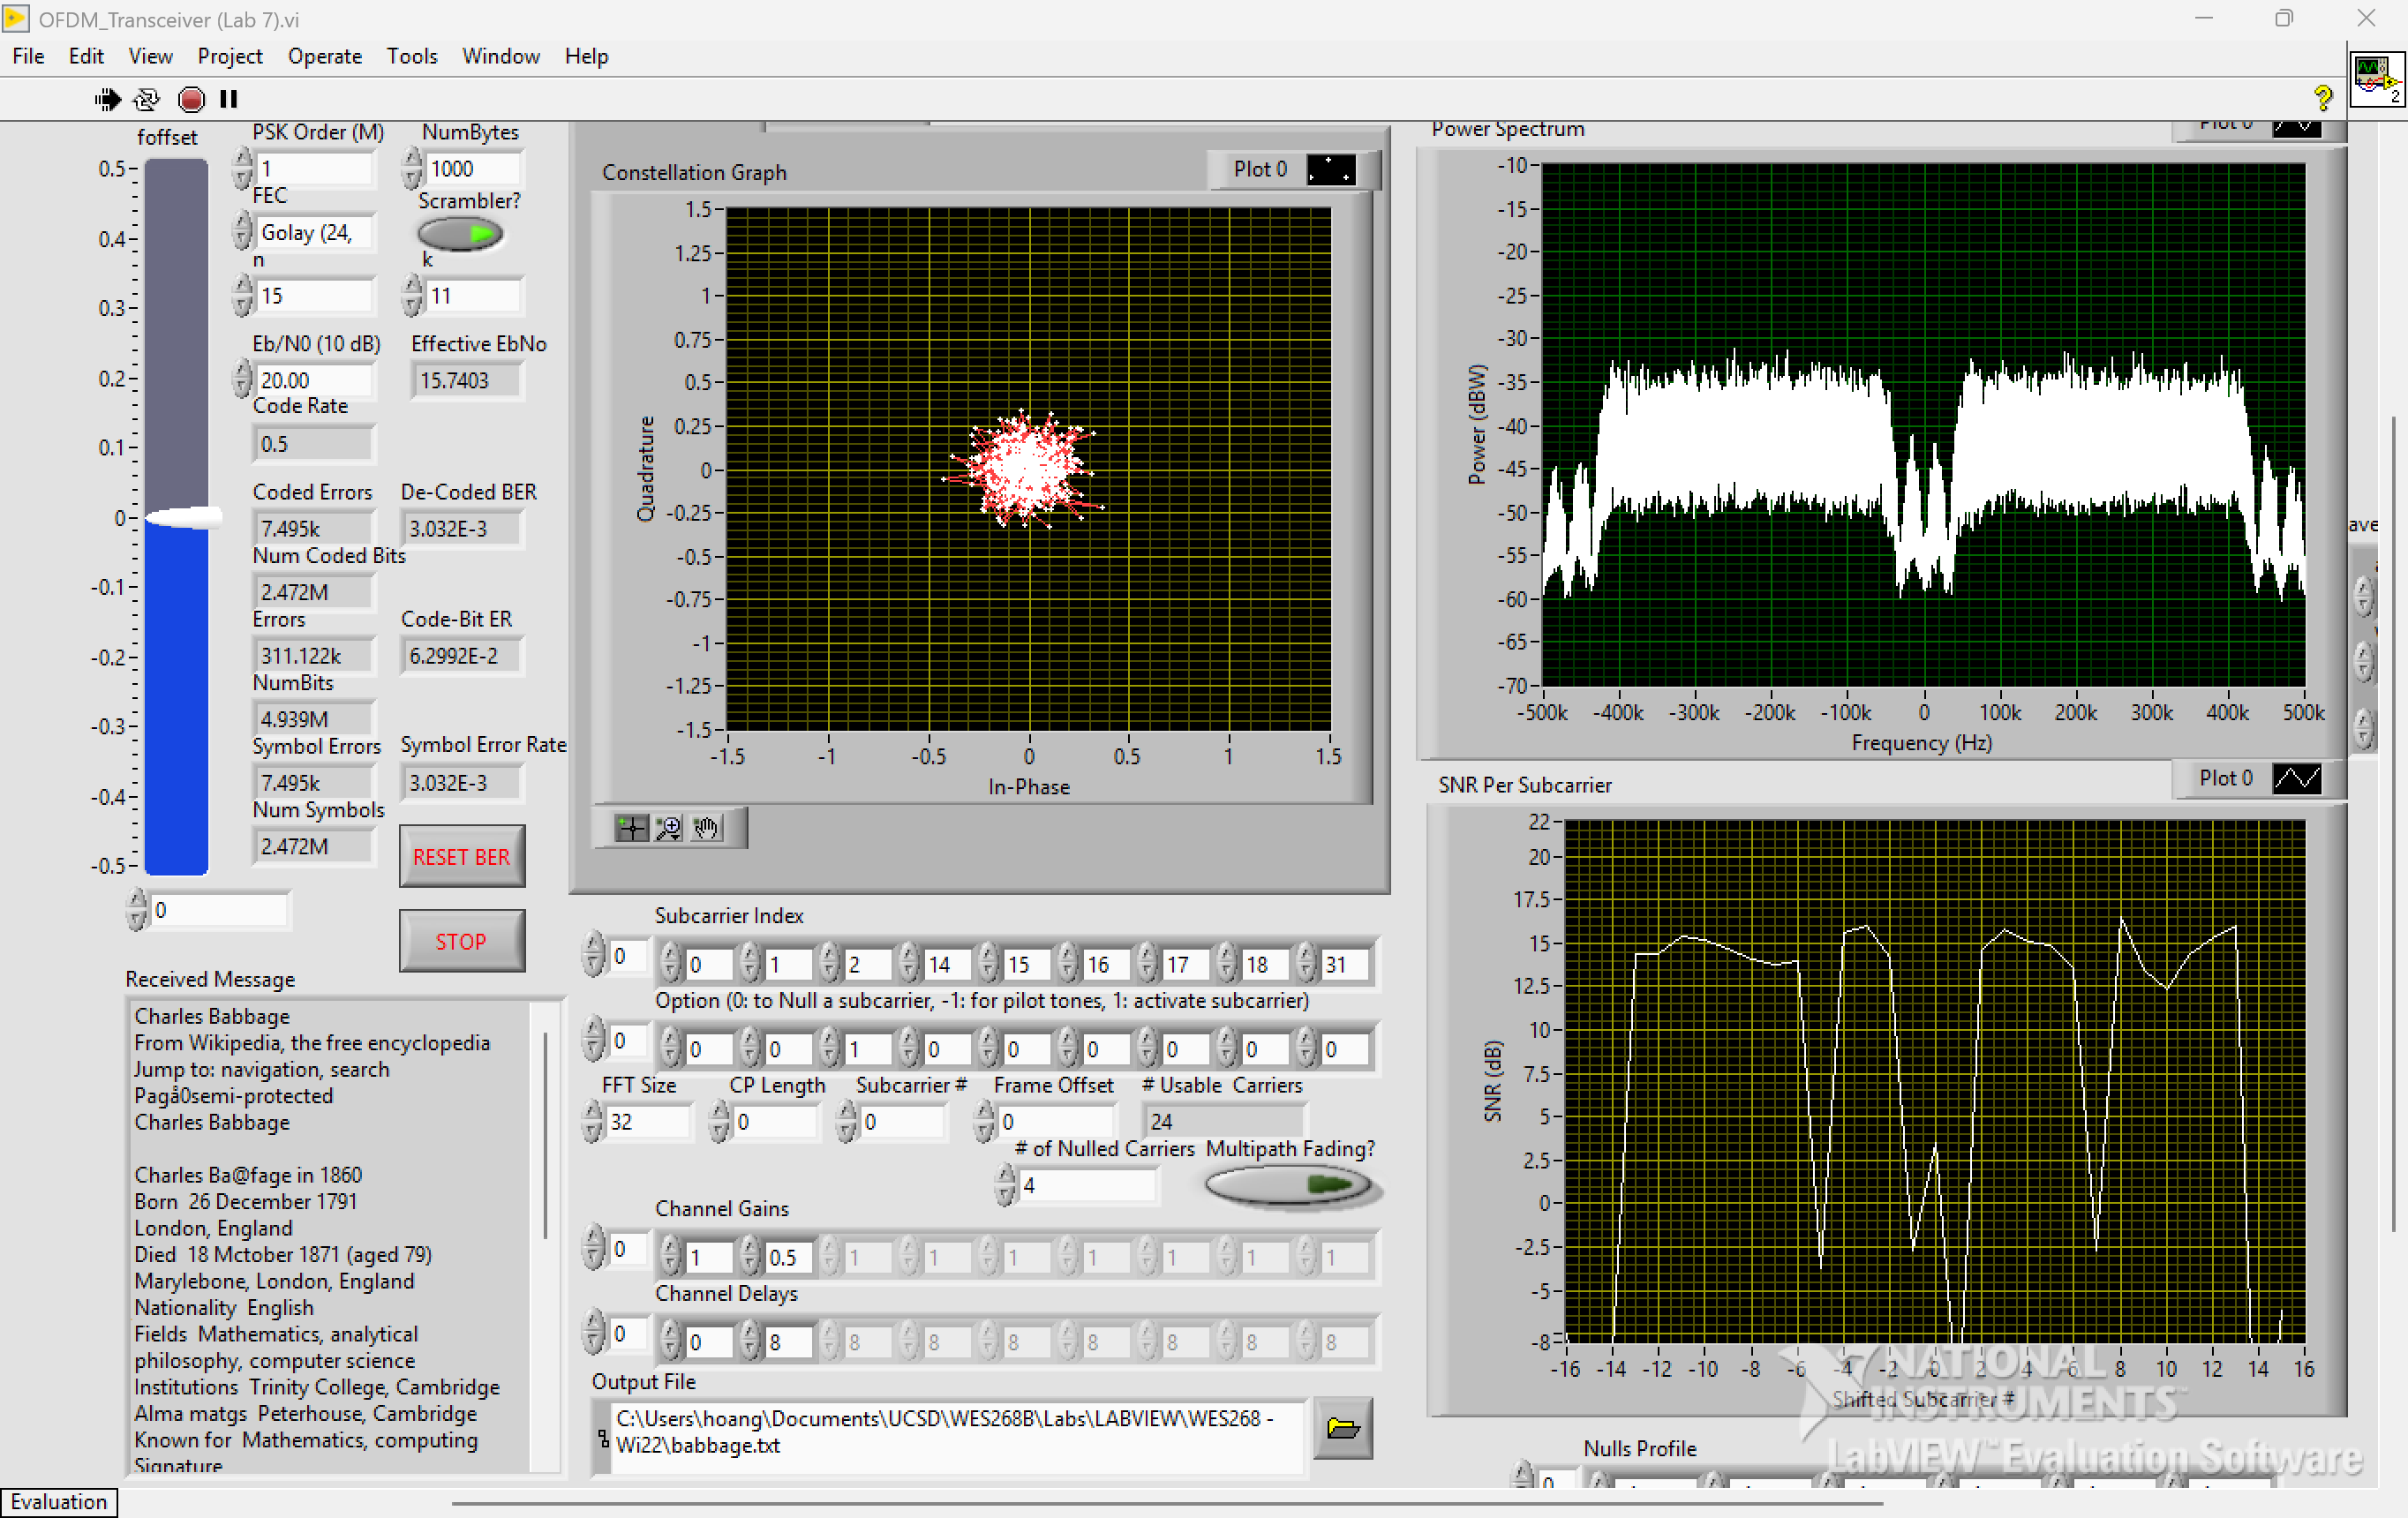
\includegraphics[width=0.7\textwidth]{lab_ss/WES268B_Lab7_Part1-1-3_FEC-Golay24_nullCarriers-4.png}
    \caption{Lab 7 - 4 Nulled Subcarriers Golay (24,12)}
    %\label{f10}
\end{figure}

\begin{figure}[H]
    \centering
    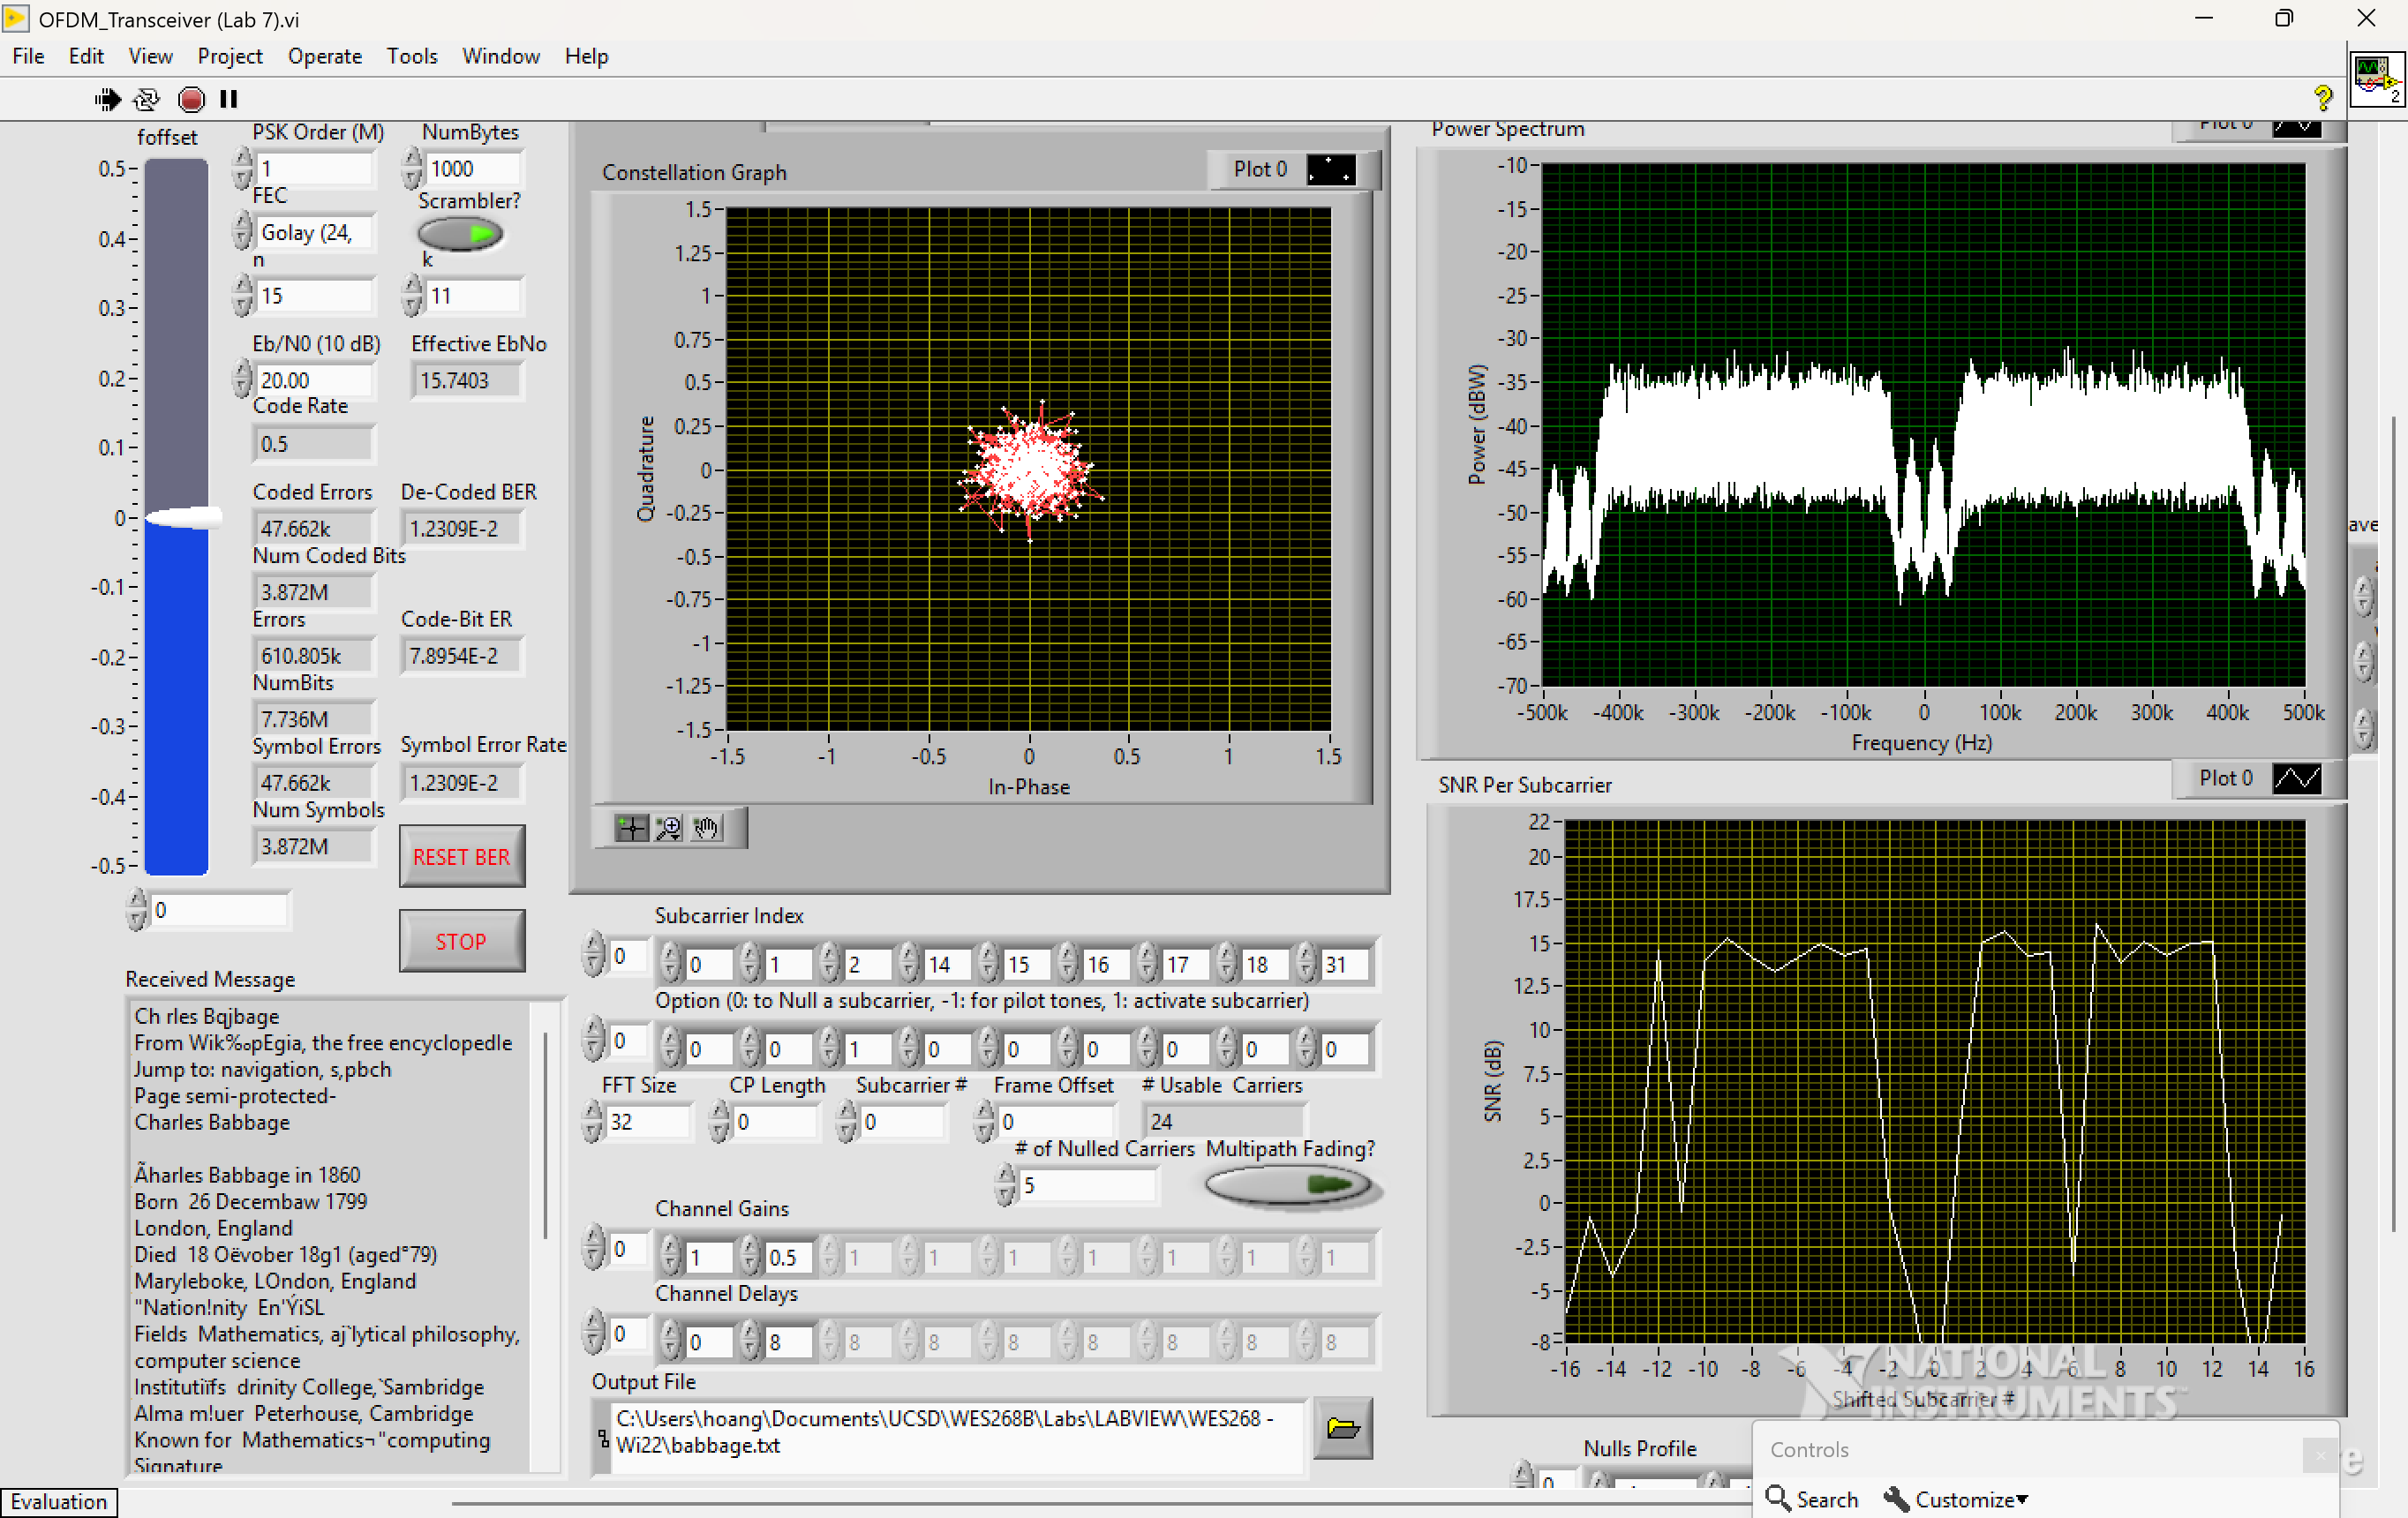
\includegraphics[width=0.7\textwidth]{lab_ss/WES268B_Lab7_Part1-1-3_FEC-Golay24_nullCarriers-5.png}
    \caption{Lab 7 - 5 Nulled Subcarriers Golay (24,12)}
    %\label{f11}
\end{figure}

\begin{figure}[H]
    \centering
    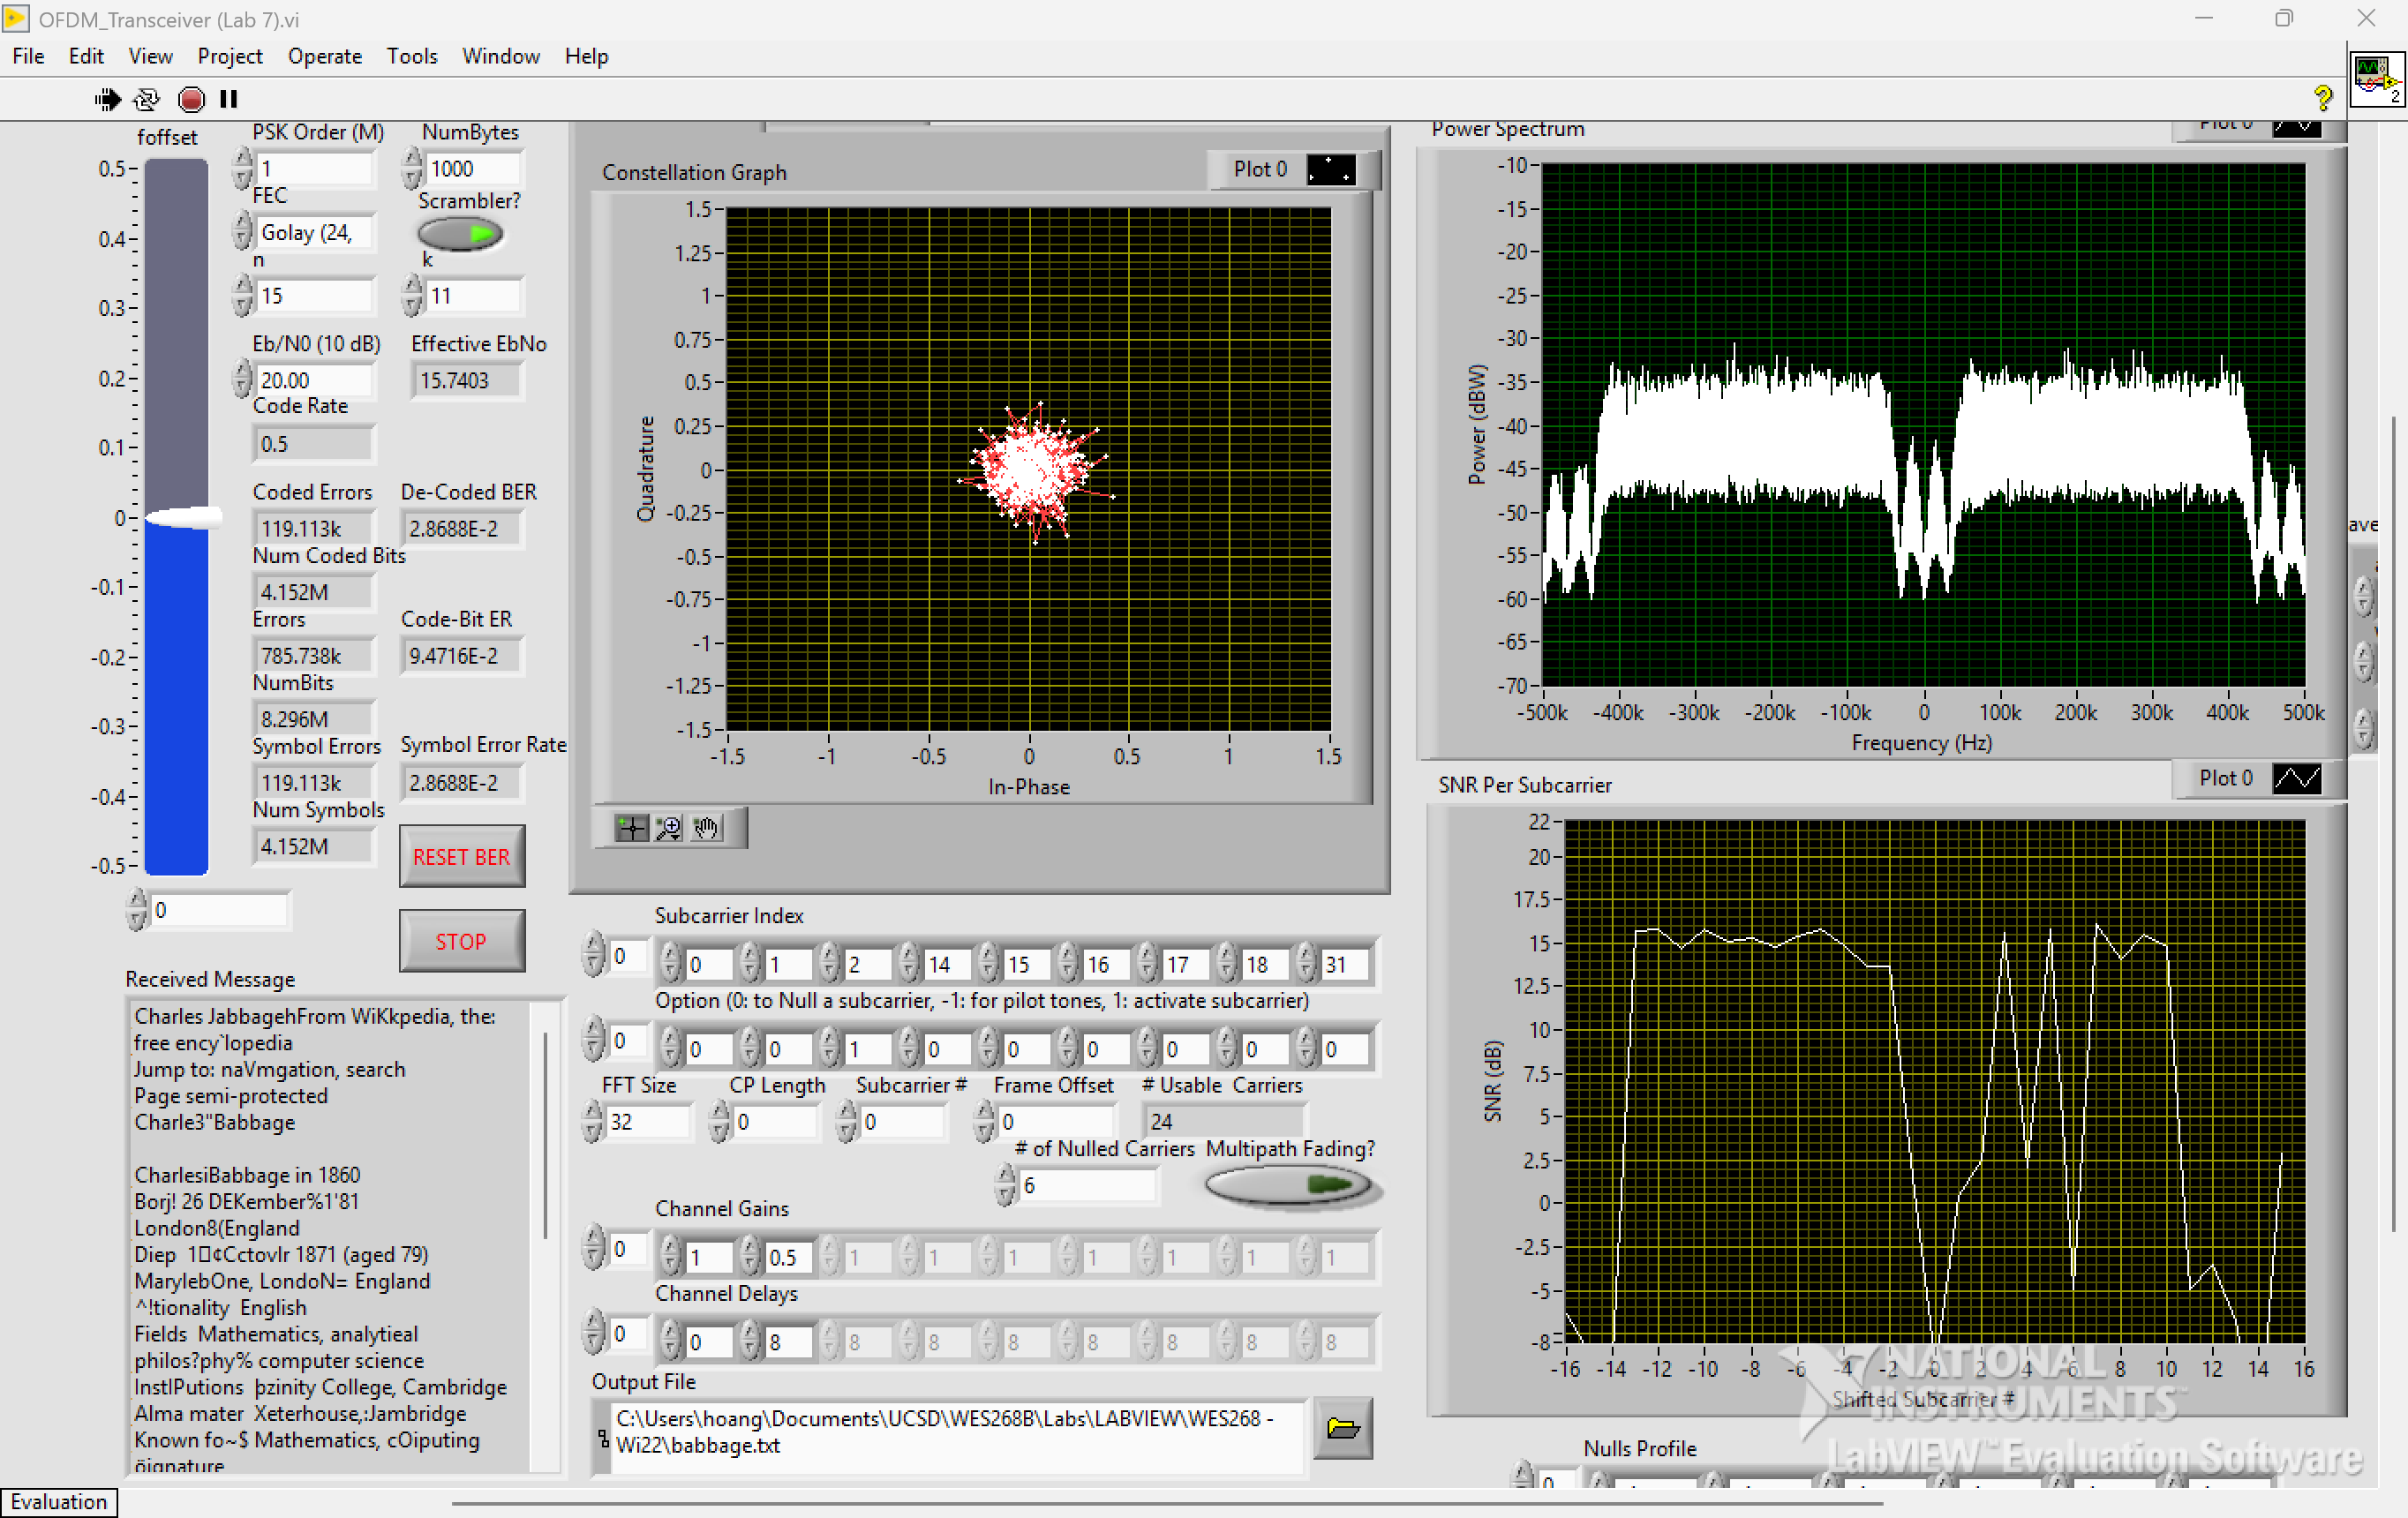
\includegraphics[width=0.7\textwidth]{lab_ss/WES268B_Lab7_Part1-1-3_FEC-Golay24_nullCarriers-6.png}
    \caption{Lab 7 - 6 Nulled Subcarriers Golay (24,12)}
    %\label{f12}
\end{figure}

% 1.1.4
\subsubsection{ }

% 1.1.5
\subsubsection{ }

% 1.1.6
\subsubsection{ }
\begin{figure}[H]
    \centering
    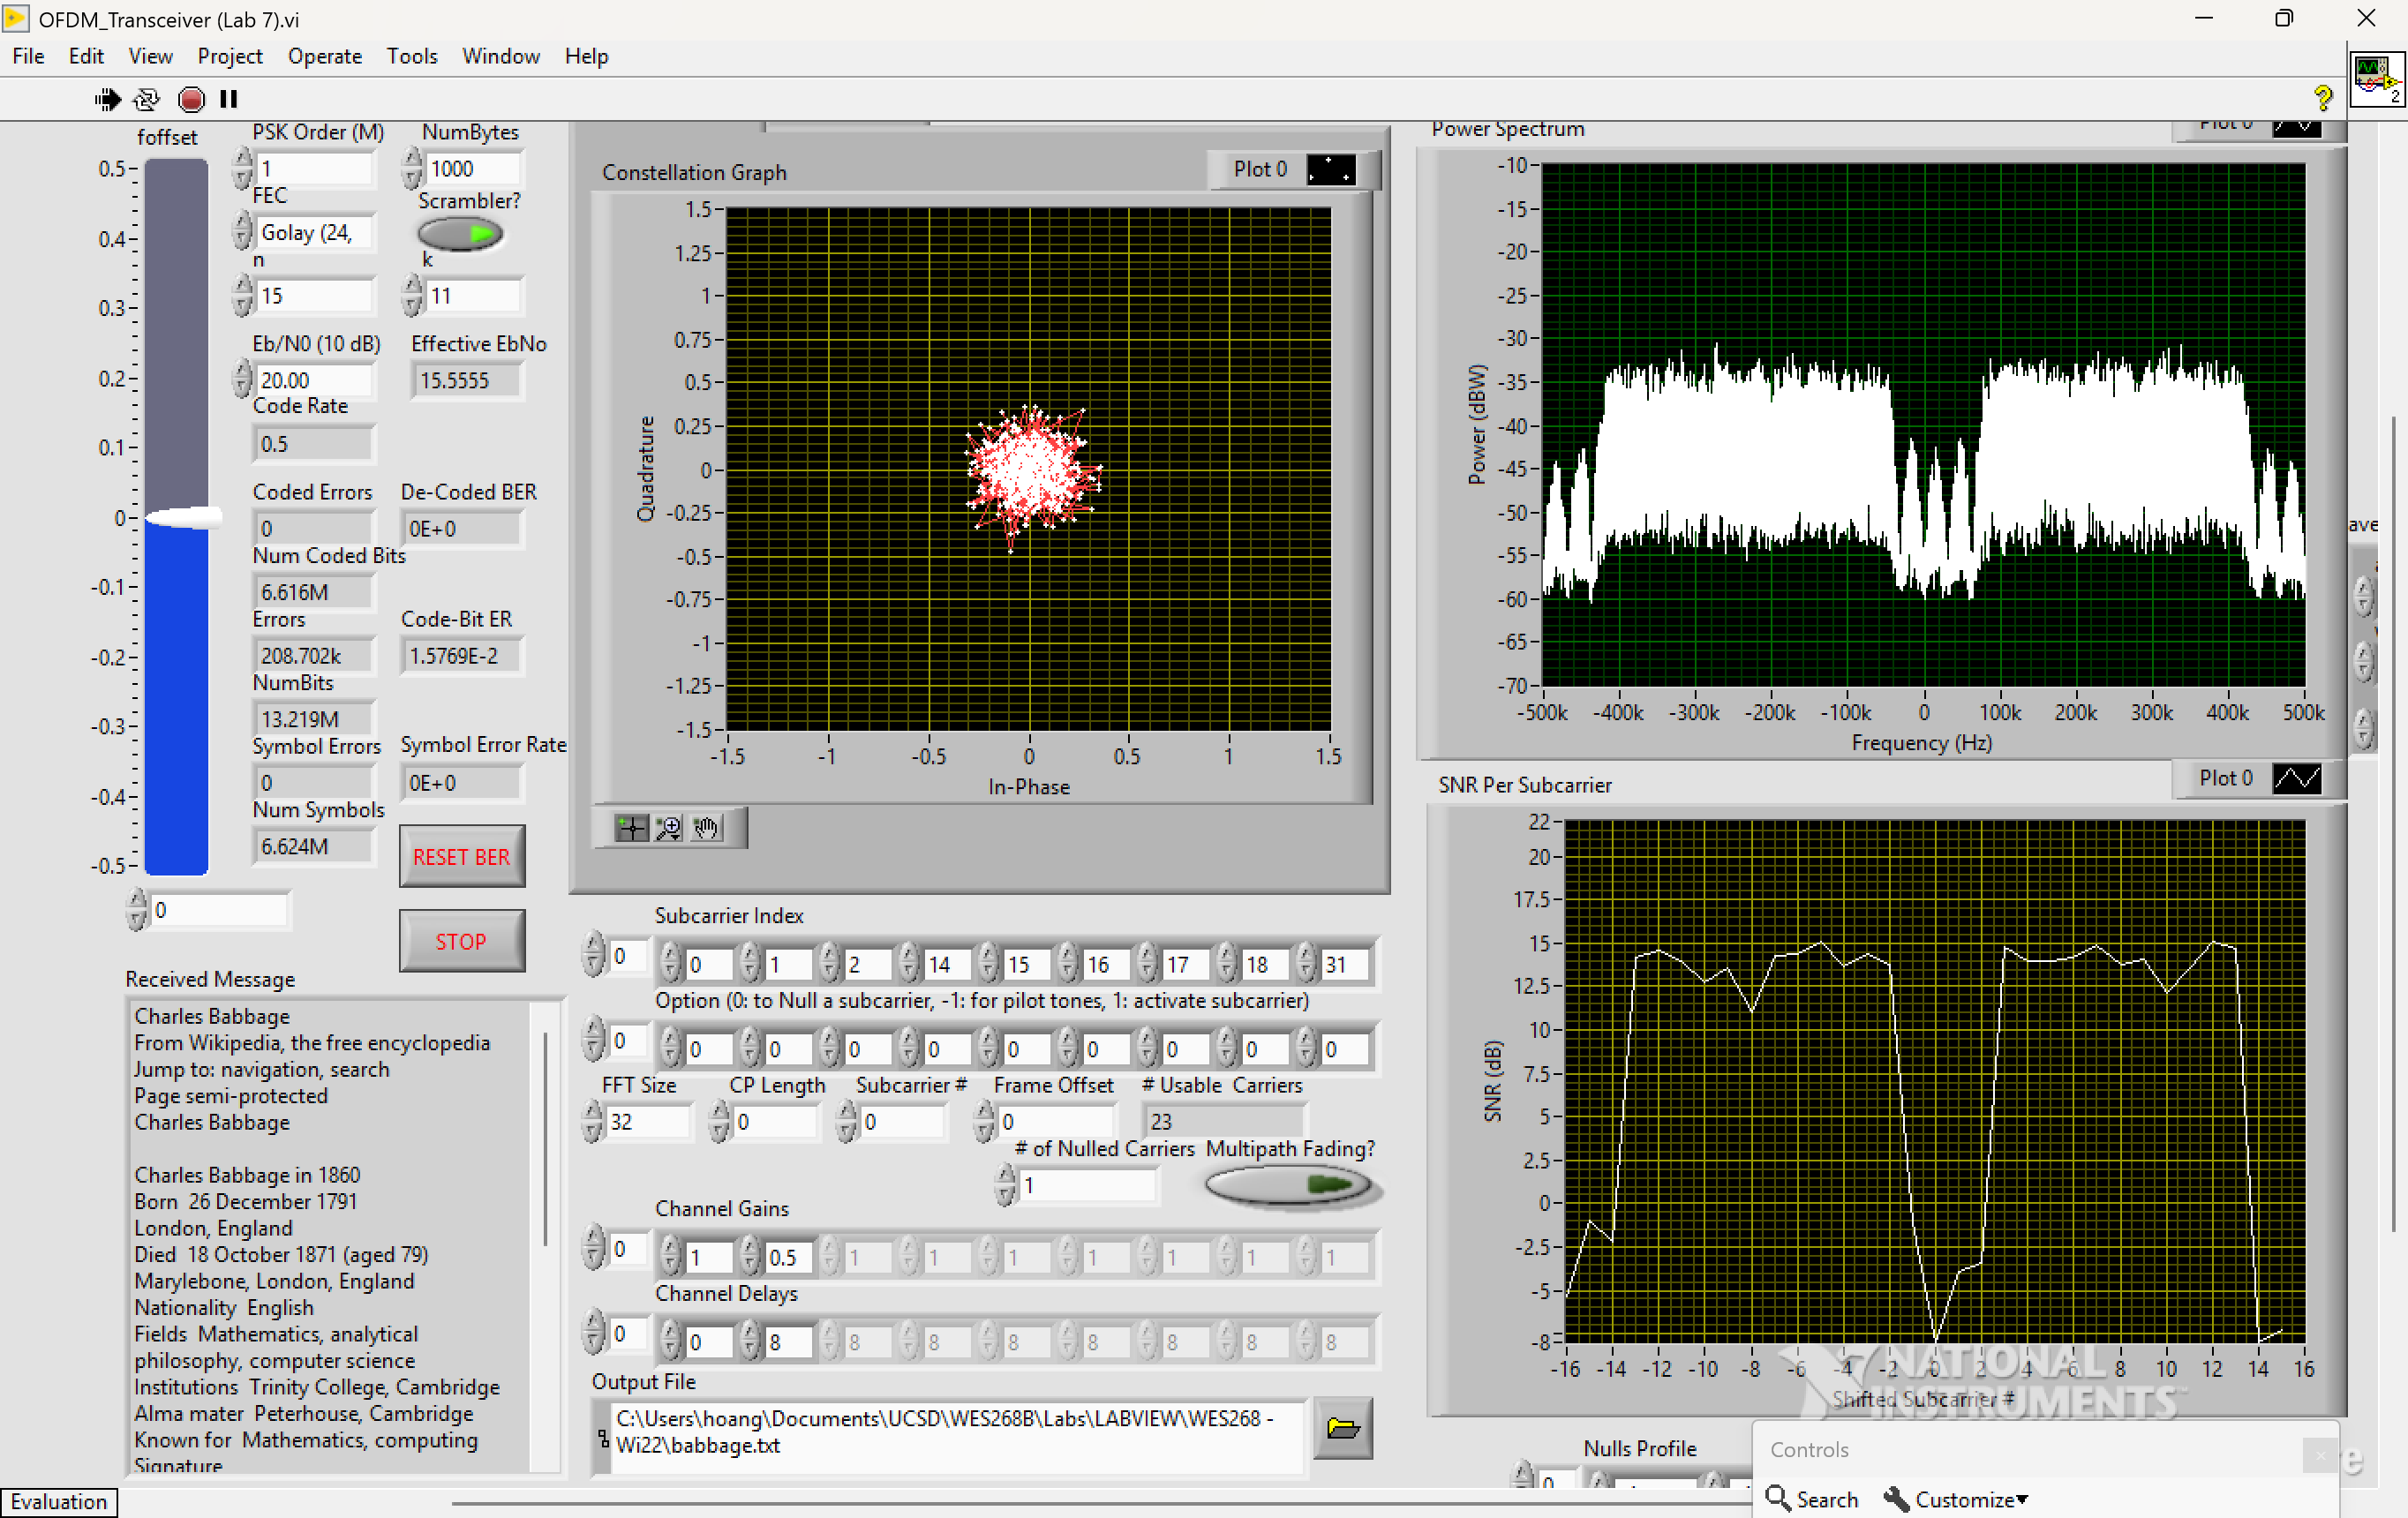
\includegraphics[width=0.7\textwidth]{lab_ss/WES268B_Lab7_Part1-1-6_FEC-Golay24_nullCarriers-1_usableCarriers-23_BER-0.png}
    \caption{Lab 7 - 1 Nulled Subcarrier Golay (24,12) 23 Usable Carriers}
    %\label{f13}
\end{figure}

\begin{figure}[H]
    \centering
    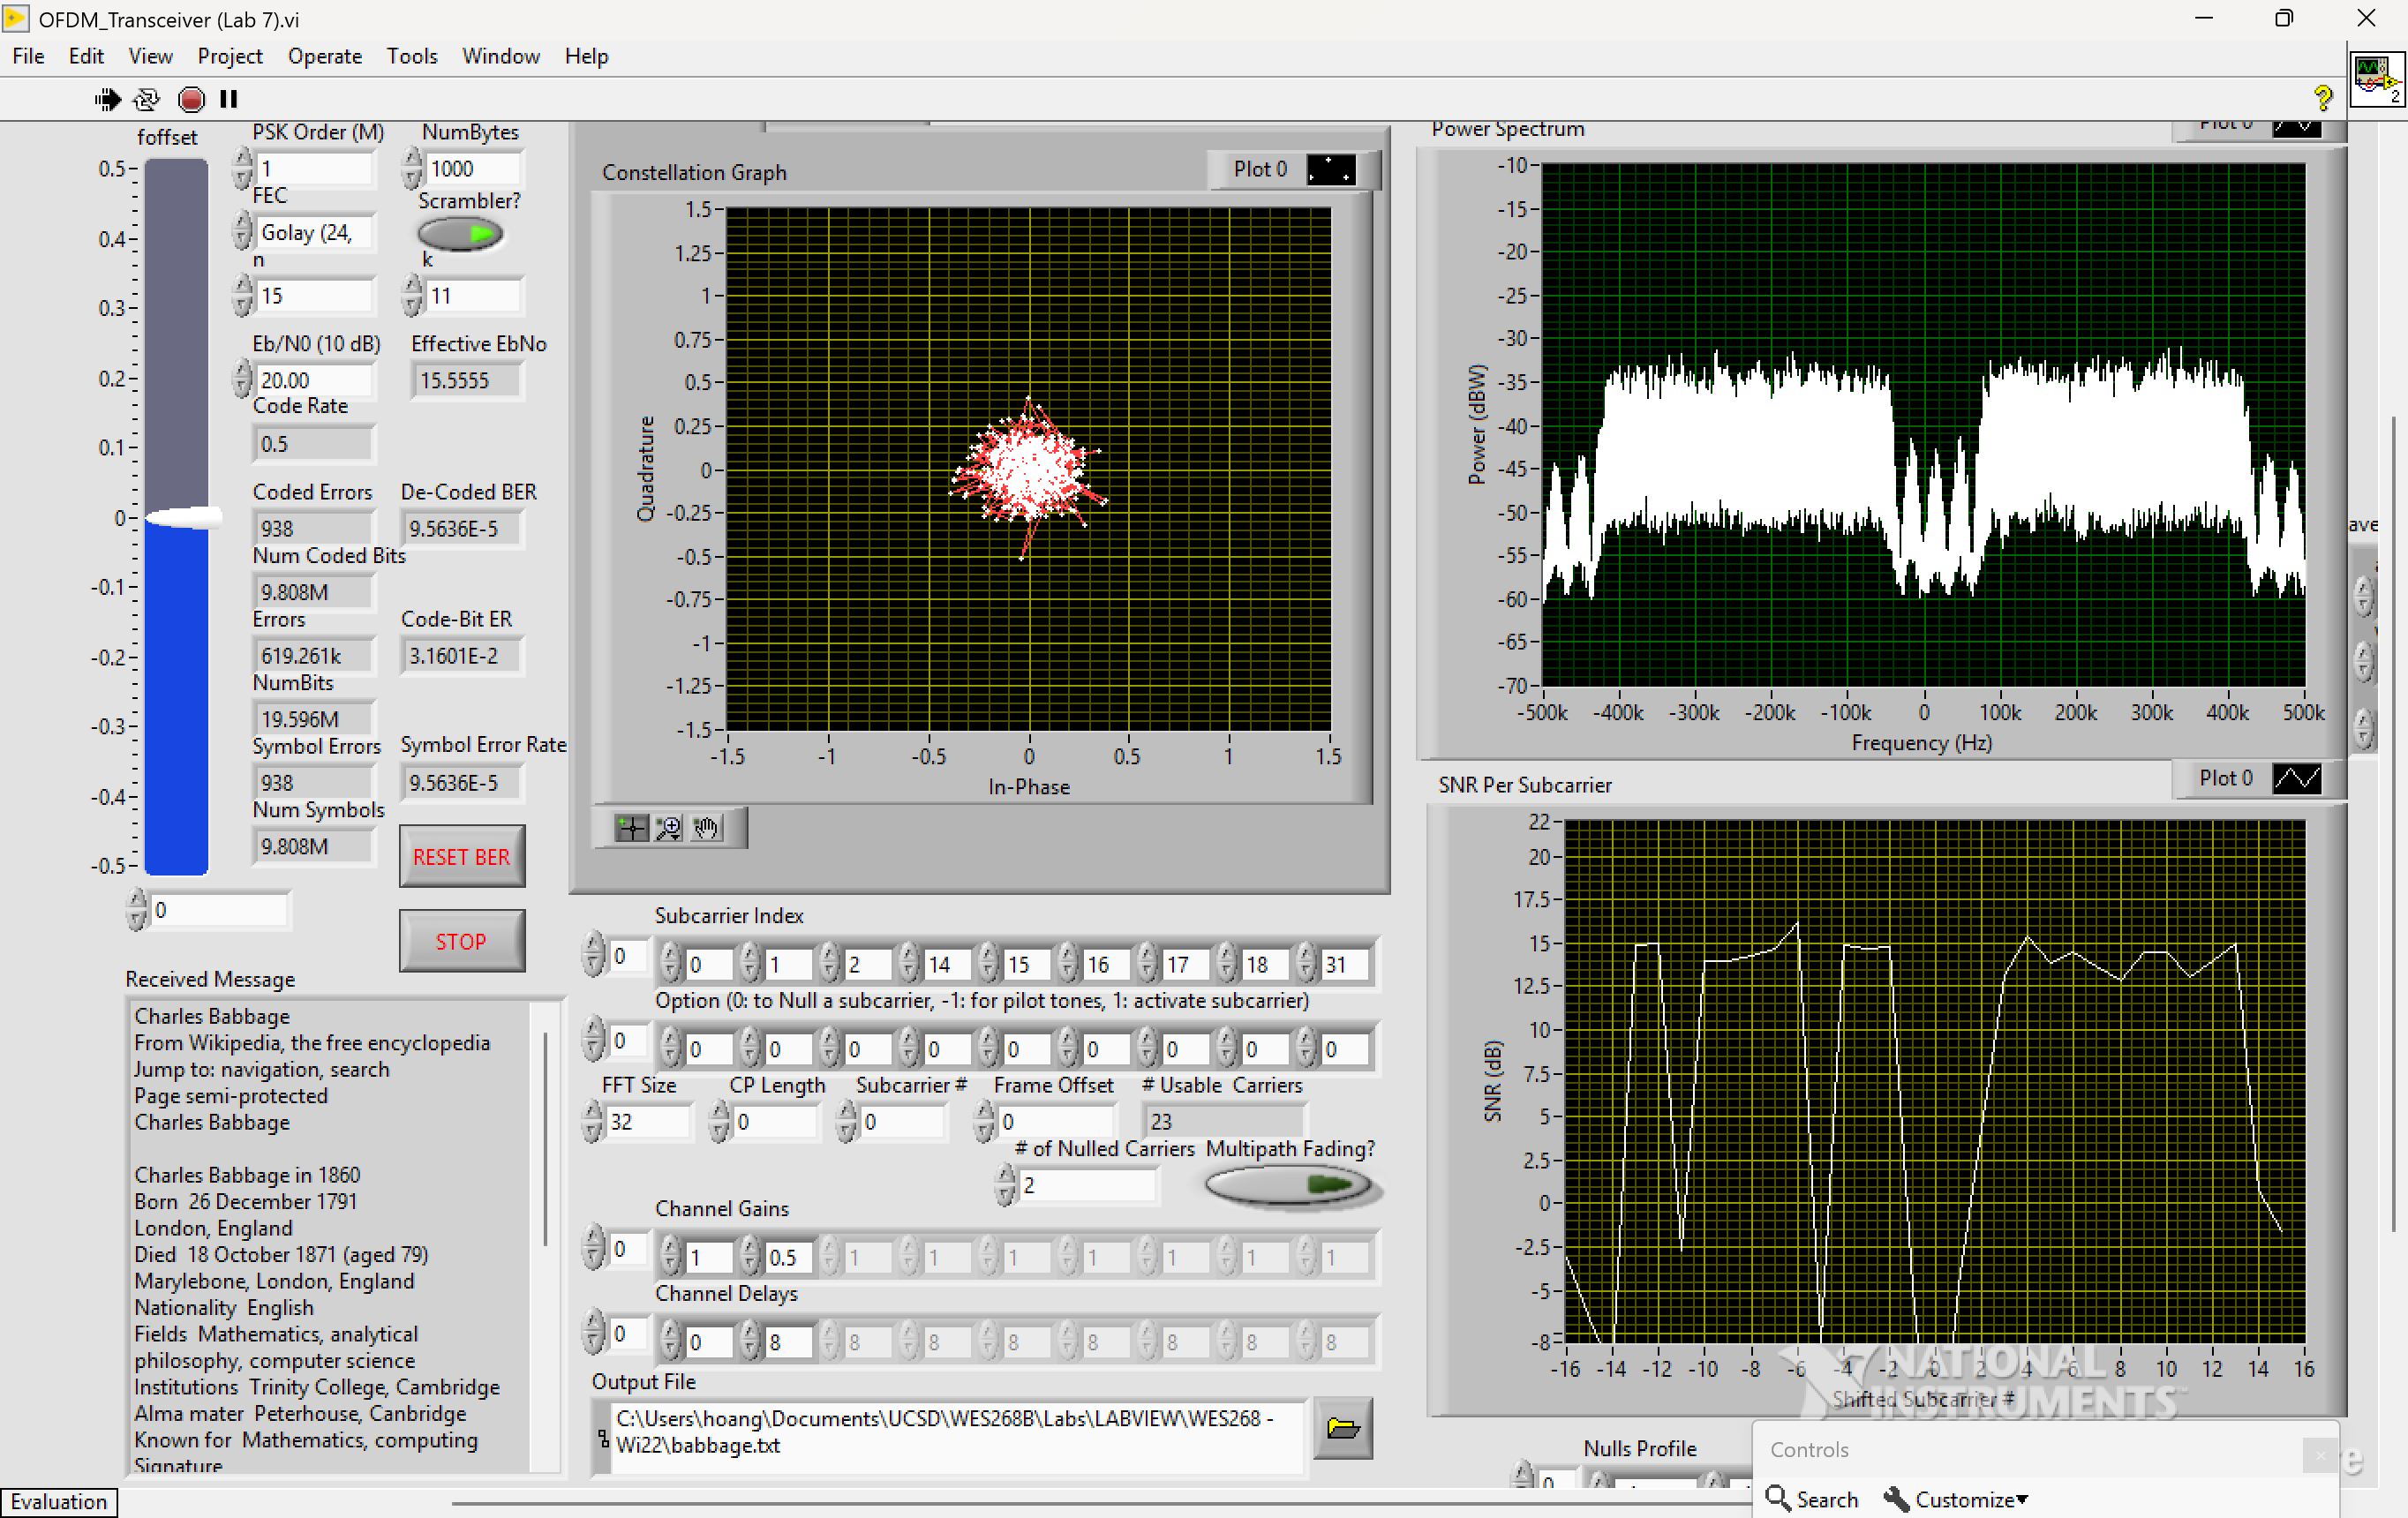
\includegraphics[width=0.7\textwidth]{lab_ss/WES268B_Lab7_Part1-1-6_FEC-Golay24_nullCarriers-2_usableCarriers-23.png}
    \caption{Lab 7 - 2 Nulled Subcarriers Golay (24,12) 23 Usable Carriers}
    %\label{f14}
\end{figure}

\begin{figure}[H]
    \centering
    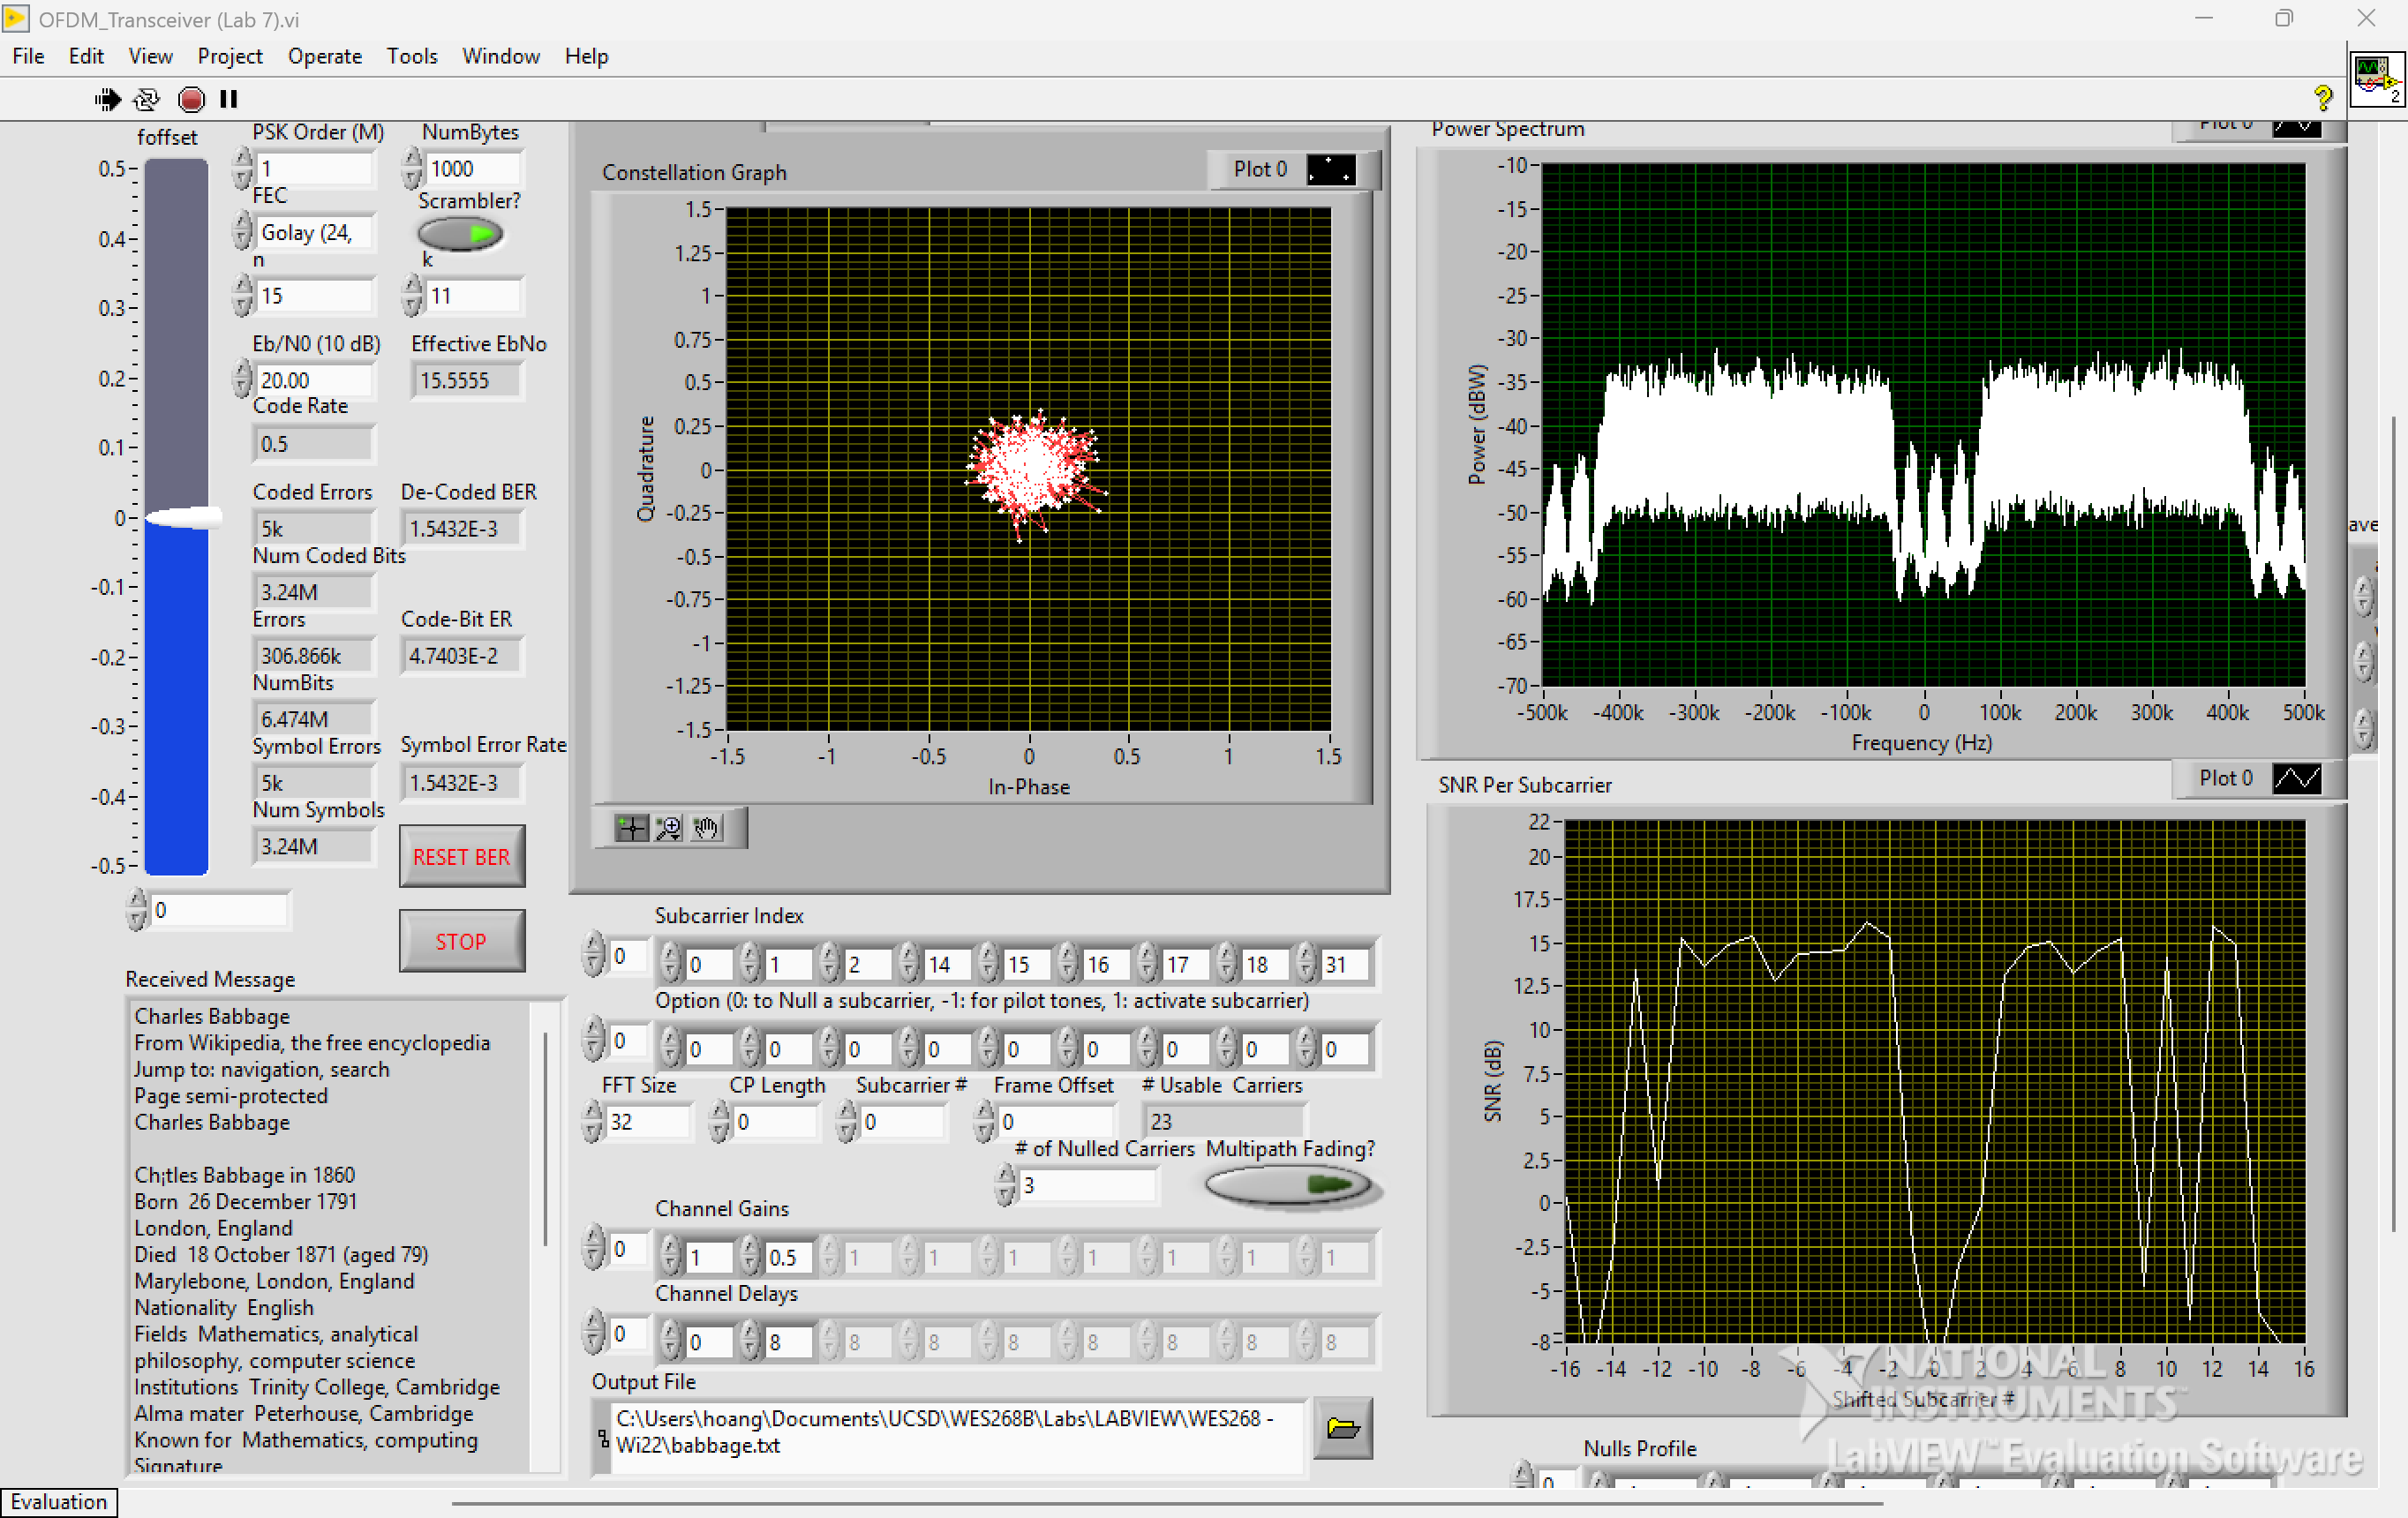
\includegraphics[width=0.7\textwidth]{lab_ss/WES268B_Lab7_Part1-1-6_FEC-Golay24_nullCarriers-3_usableCarriers-23.png}
    \caption{Lab 7 - 3 Nulled Subcarriers Golay (24,12) 23 Usable Carriers}
    %\label{f15}
\end{figure}

\begin{figure}[H]
    \centering
    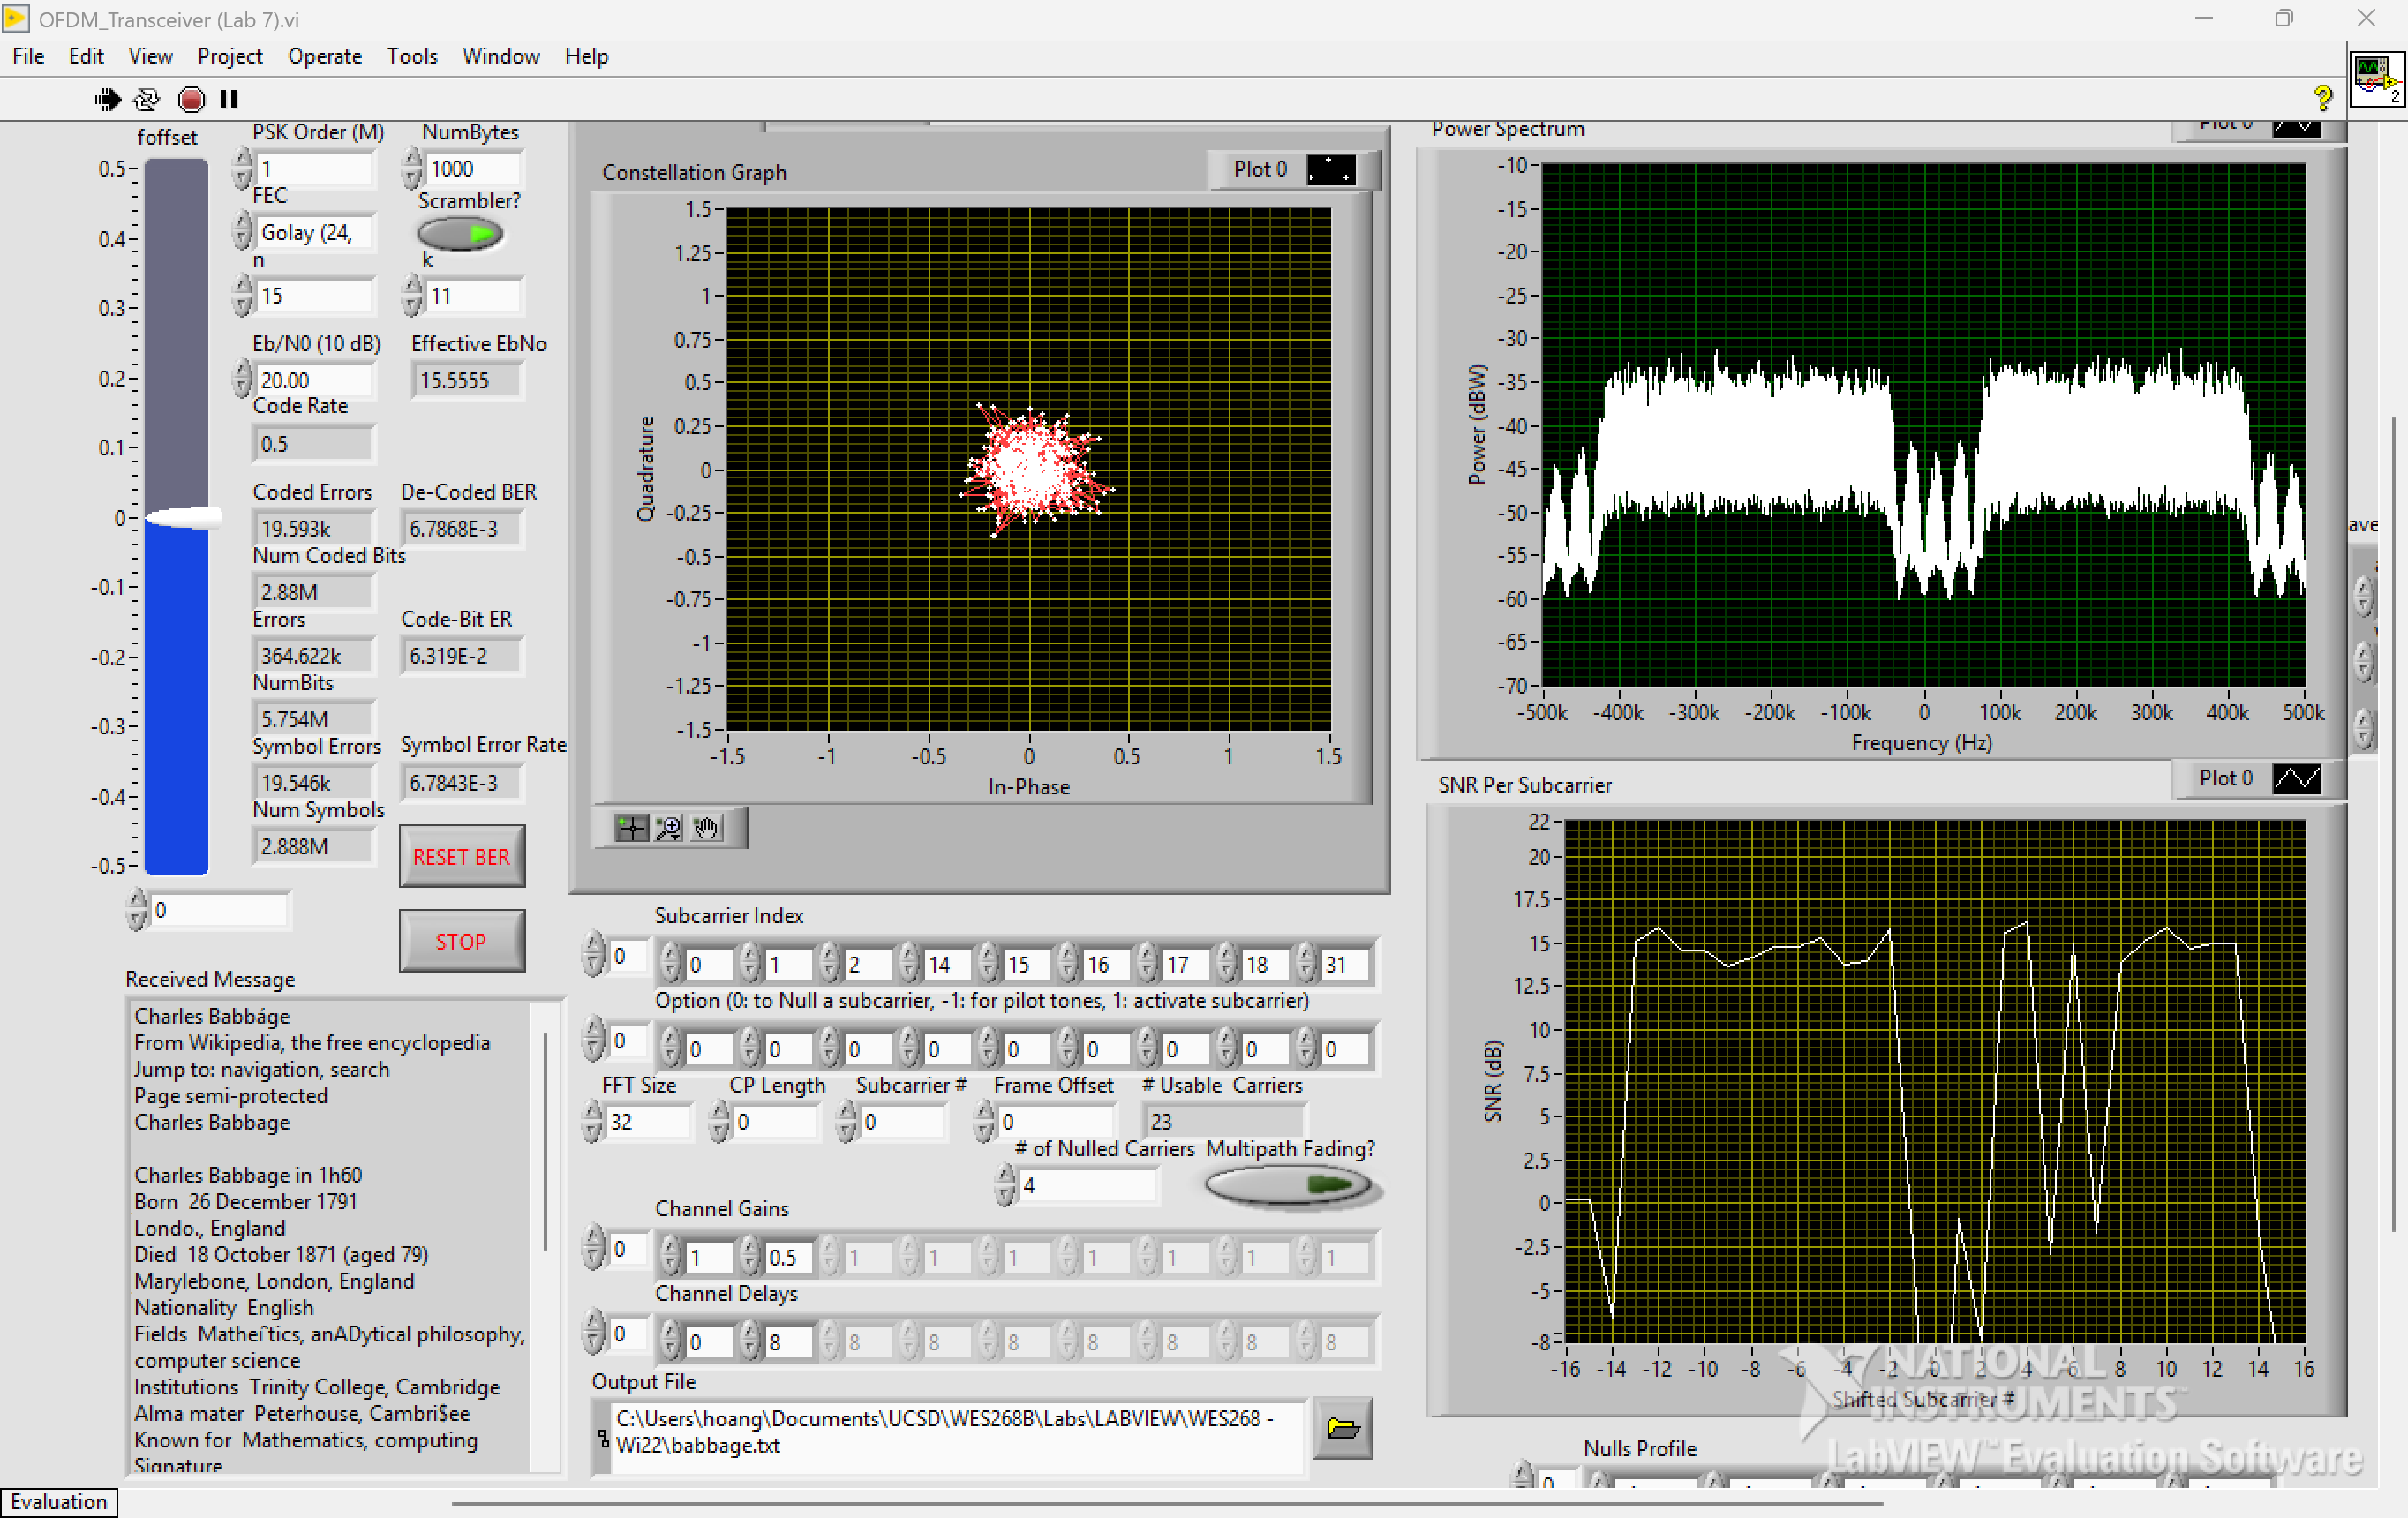
\includegraphics[width=0.7\textwidth]{lab_ss/WES268B_Lab7_Part1-1-6_FEC-Golay24_nullCarriers-4_usableCarriers-23.png}
    \caption{Lab 7 - 4 Nulled Subcarriers Golay (24,12) 23 Usable Carriers}
    %\label{f16}
\end{figure}

\begin{figure}[H]
    \centering
    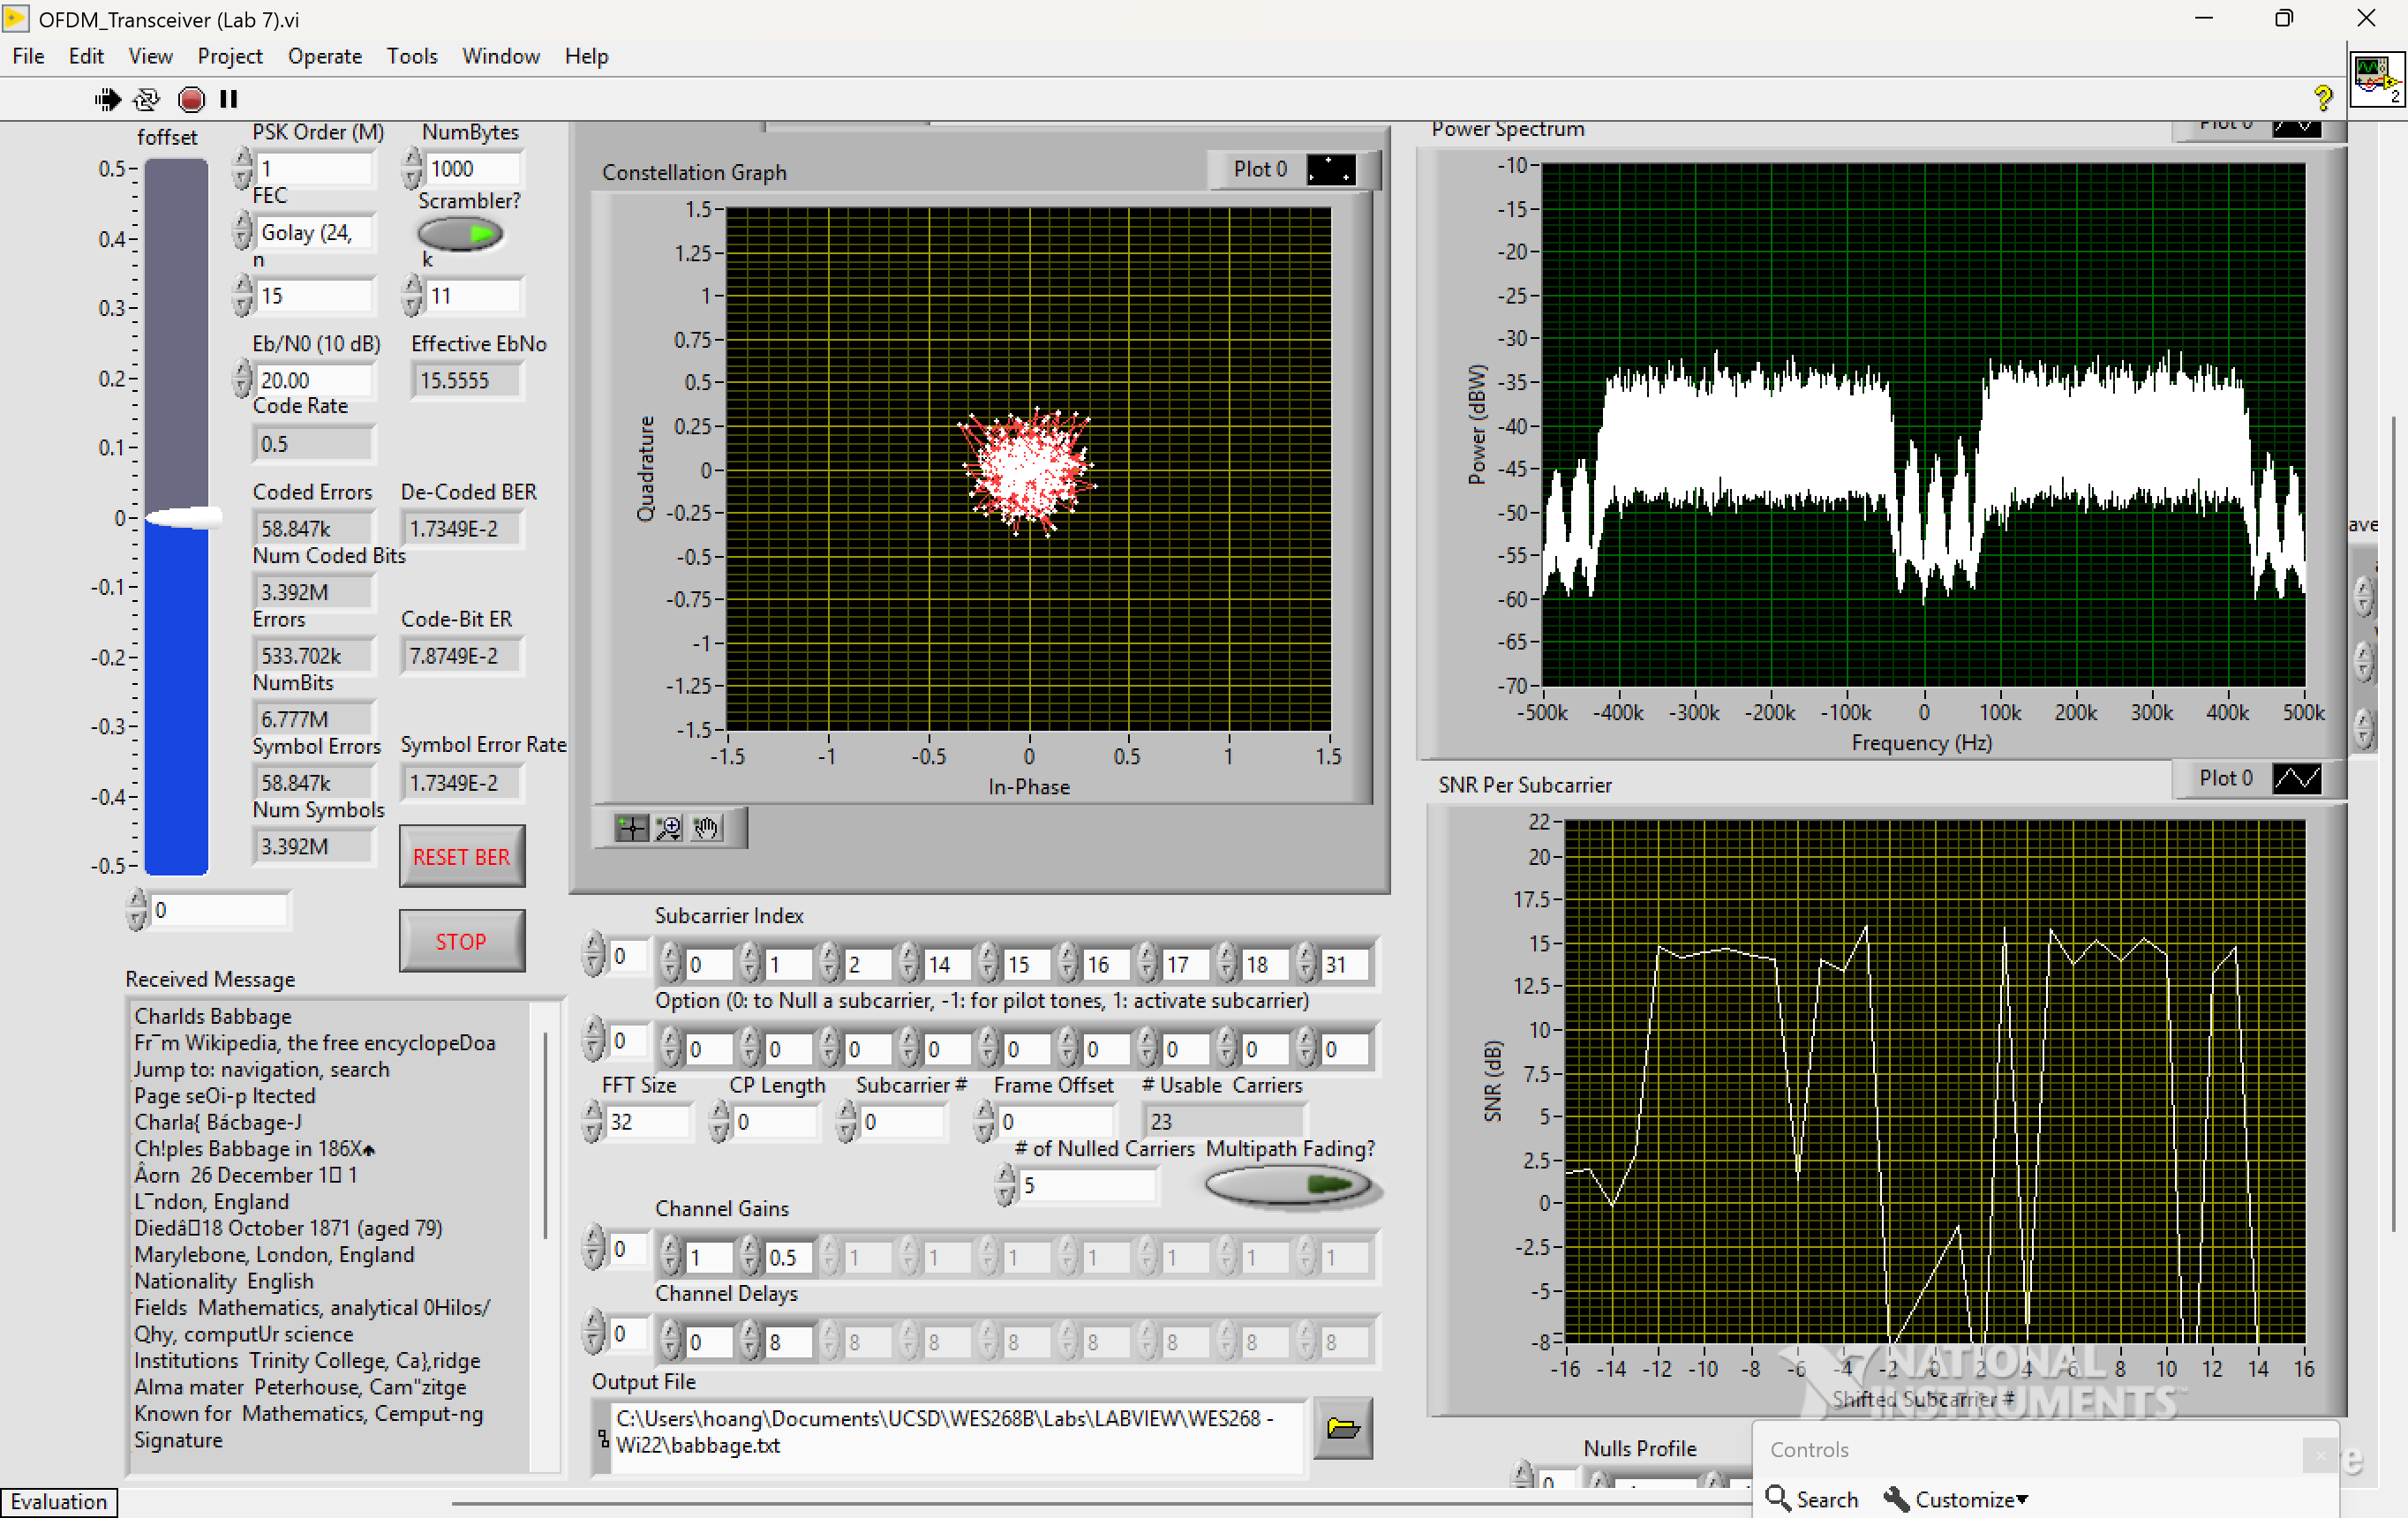
\includegraphics[width=0.7\textwidth]{lab_ss/WES268B_Lab7_Part1-1-6_FEC-Golay24_nullCarriers-5_usableCarriers-23.png}
    \caption{Lab 7 - 5 Nulled Subcarriers Golay (24,12) 23 Usable Carriers}
    %\label{f17}
\end{figure}

\begin{figure}[H]
    \centering
    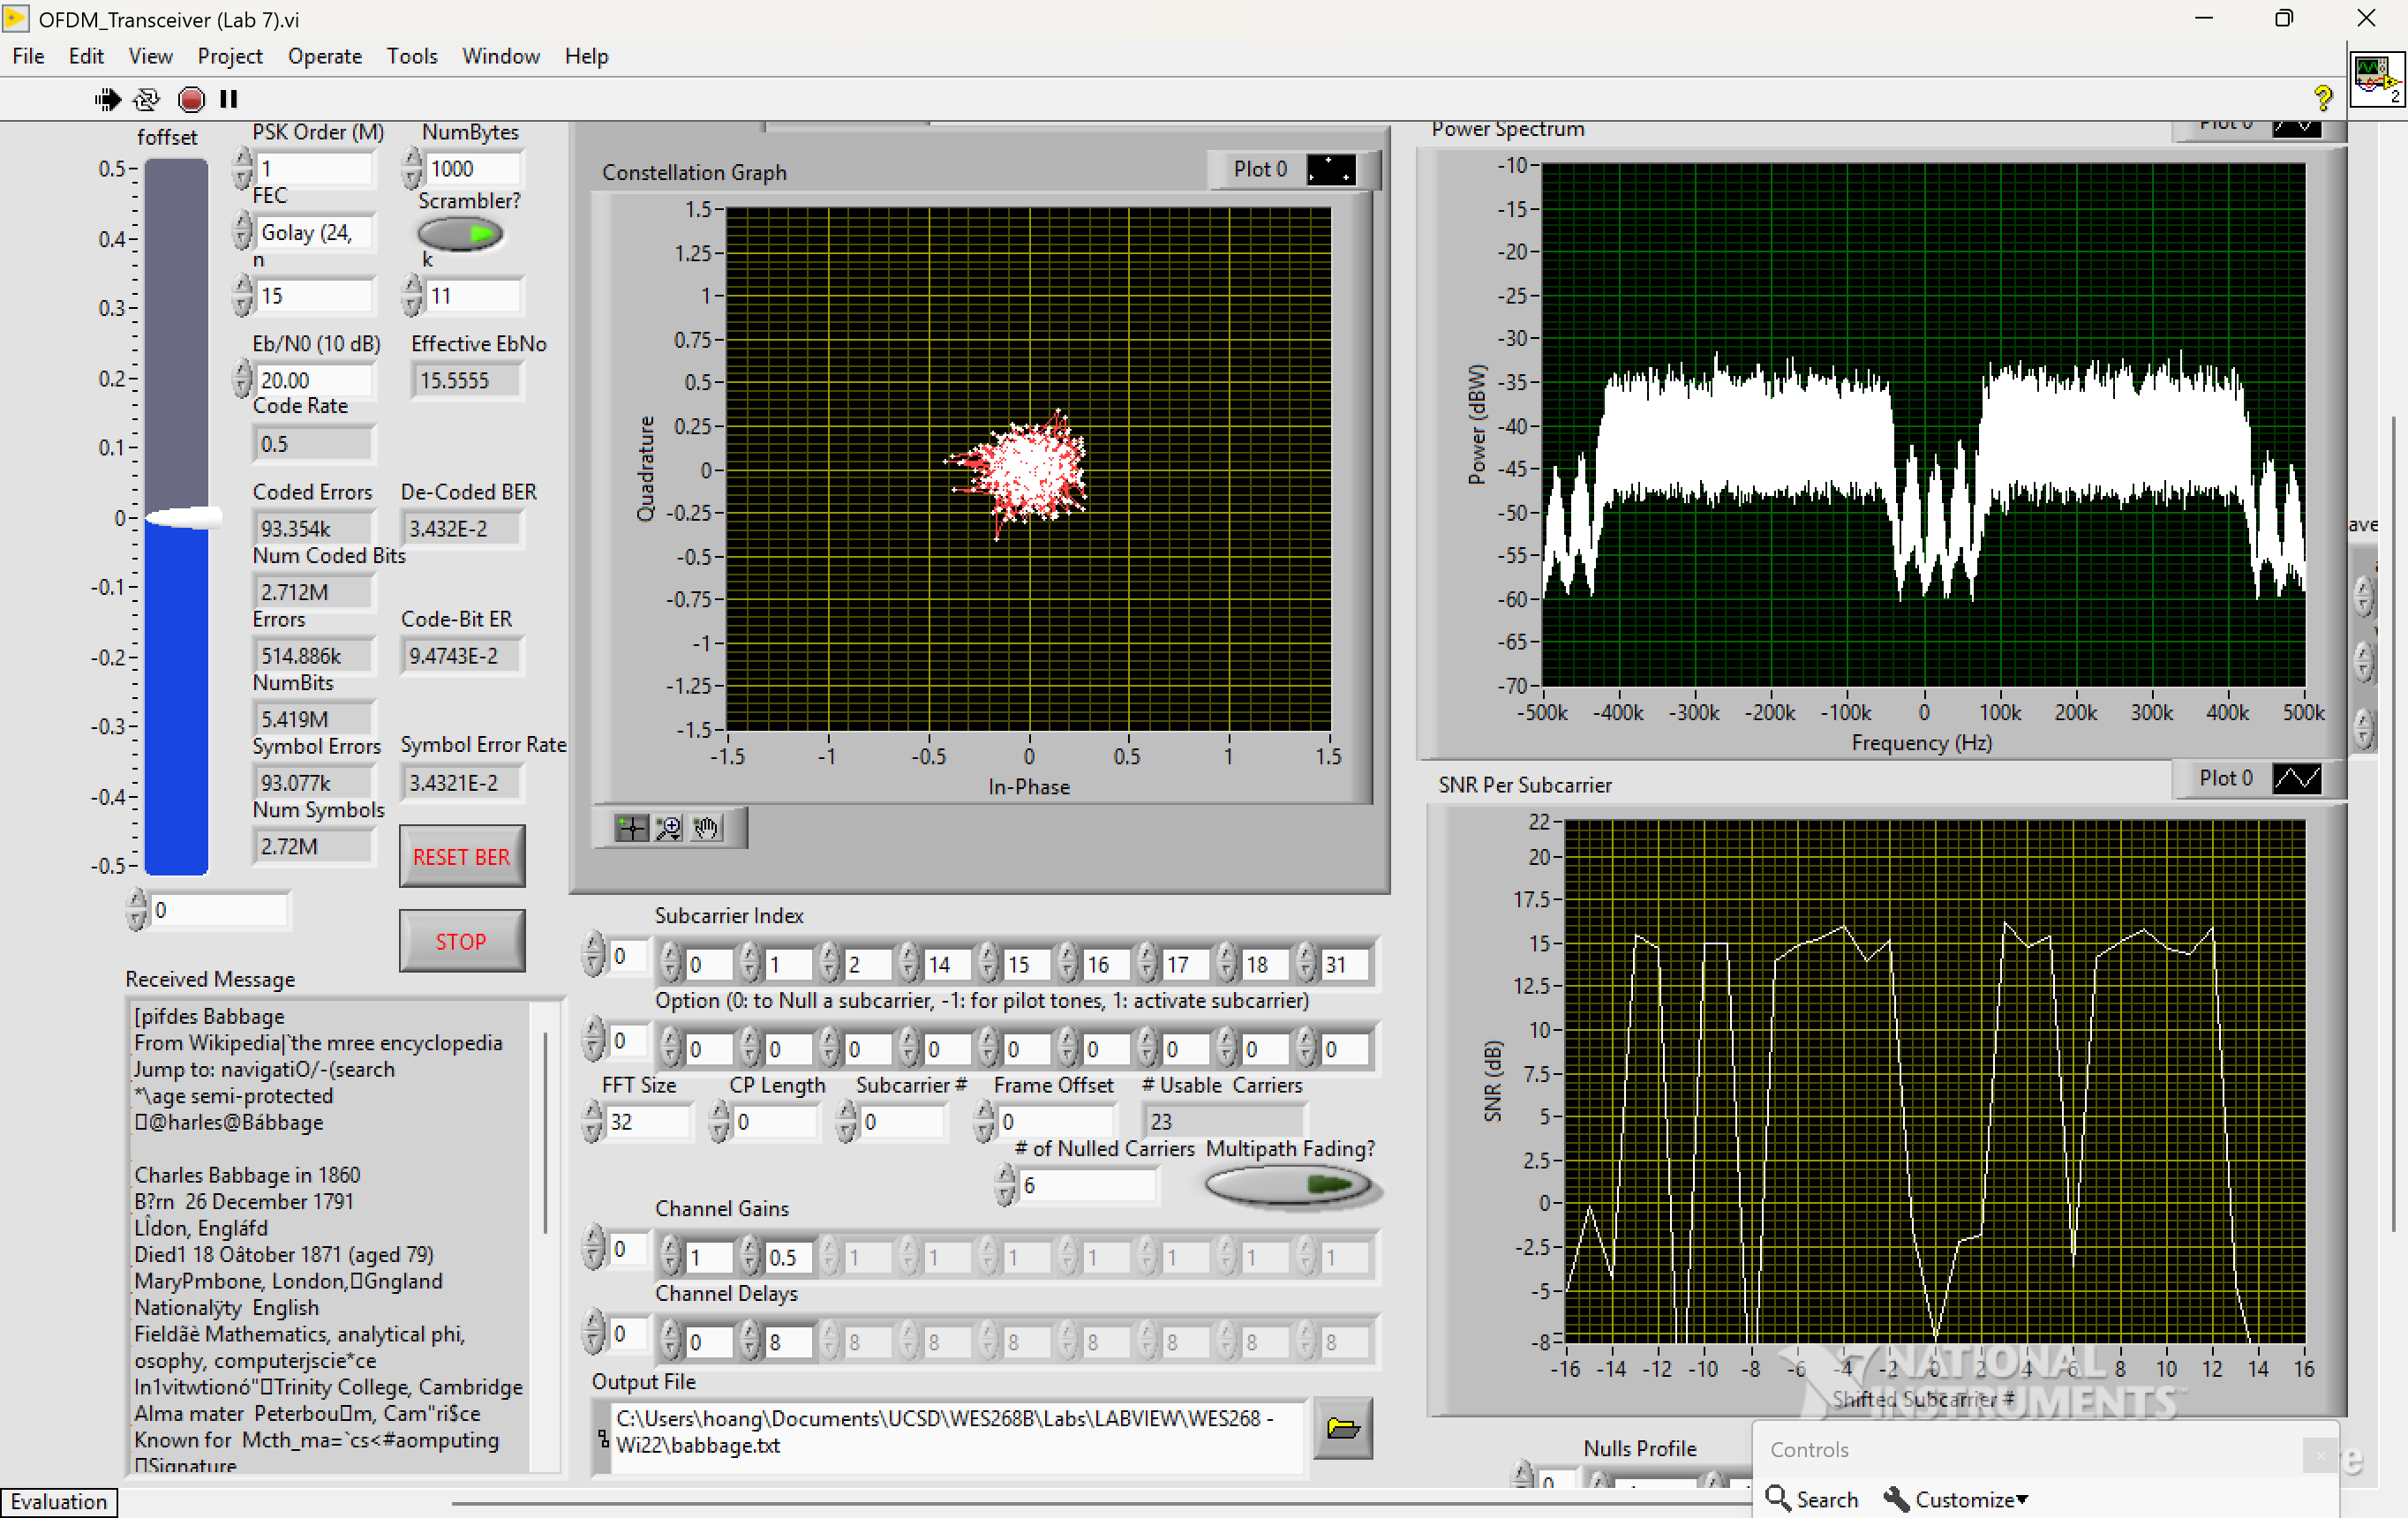
\includegraphics[width=0.7\textwidth]{lab_ss/WES268B_Lab7_Part1-1-6_FEC-Golay24_nullCarriers-6_usableCarriers-23.png}
    \caption{Lab 7 - 6 Nulled Subcarriers Golay (24,12) 23 Usable Carriers}
    %\label{f18}
\end{figure}

% 1.1.7
\subsubsection{ }
\begin{figure}[H]
    \centering
    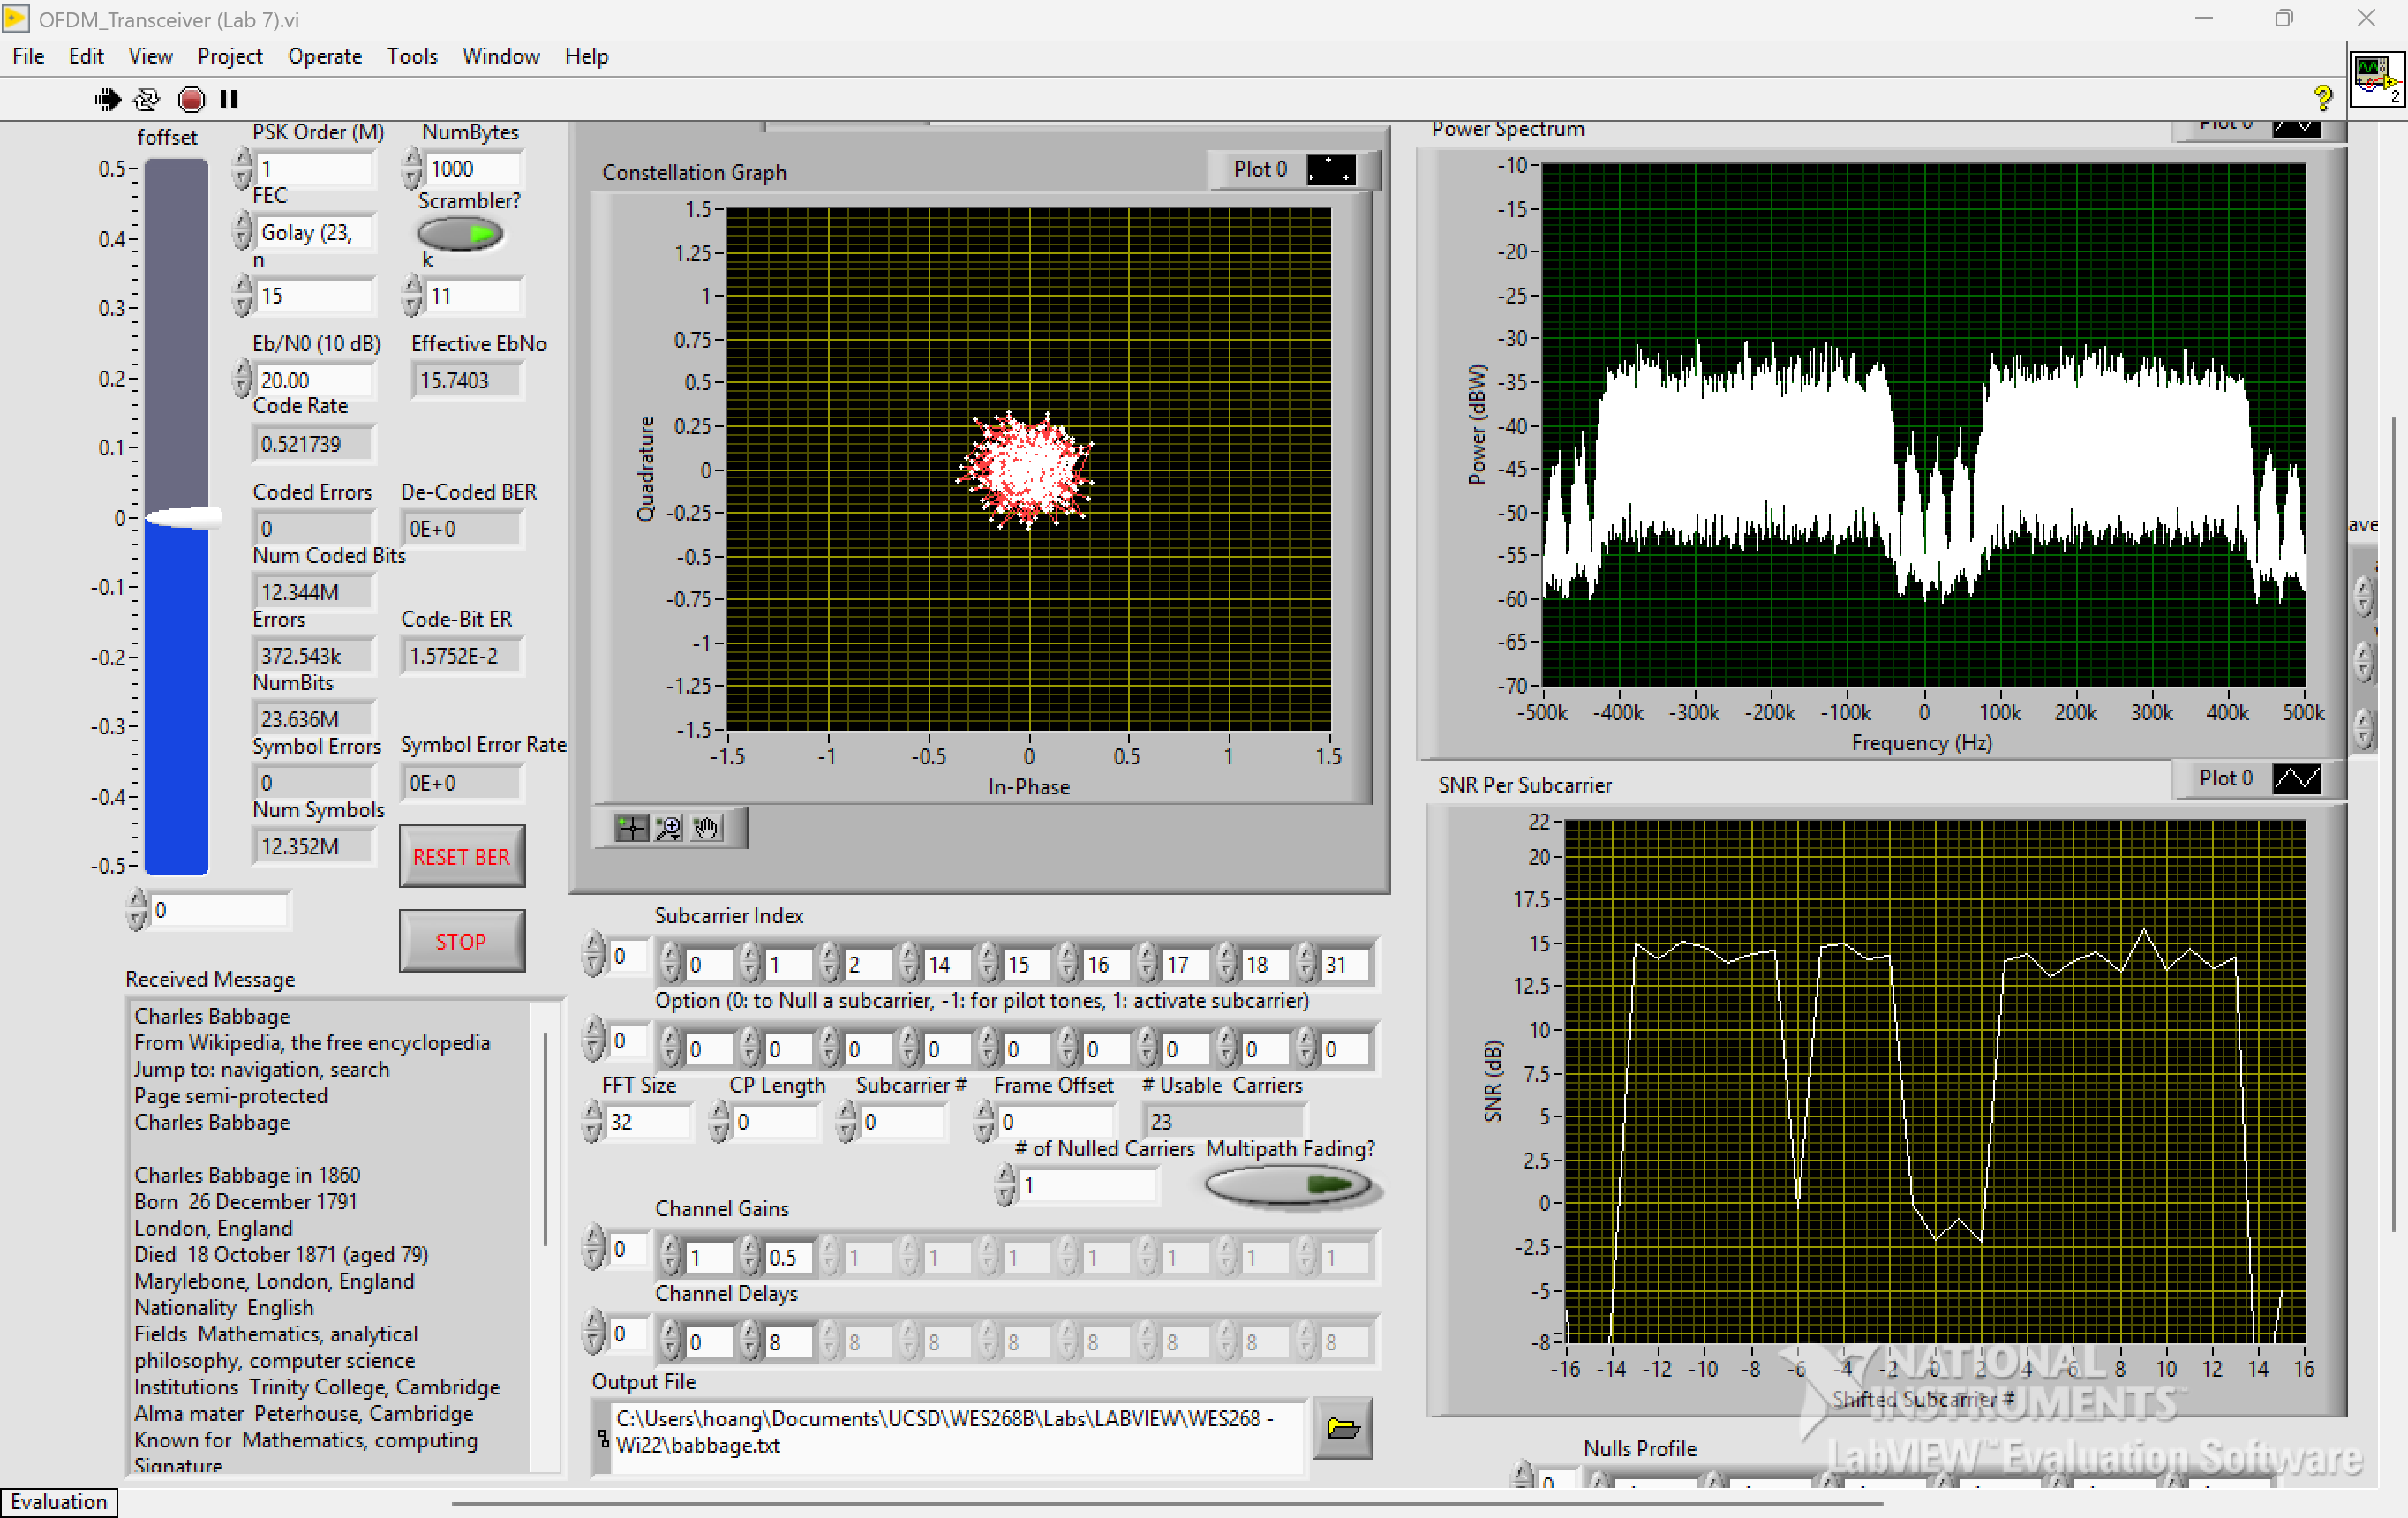
\includegraphics[width=0.7\textwidth]{lab_ss/WES268B_Lab7_Part1-1-7_FEC-Golay23_nullCarriers-1_usableCarriers-23_BER-0.png}
    \caption{Lab 7 - 1 Nulled Subcarrier Golay (23,12) 23 Usable Carriers}
    %\label{f19}
\end{figure}

\begin{figure}[H]
    \centering
    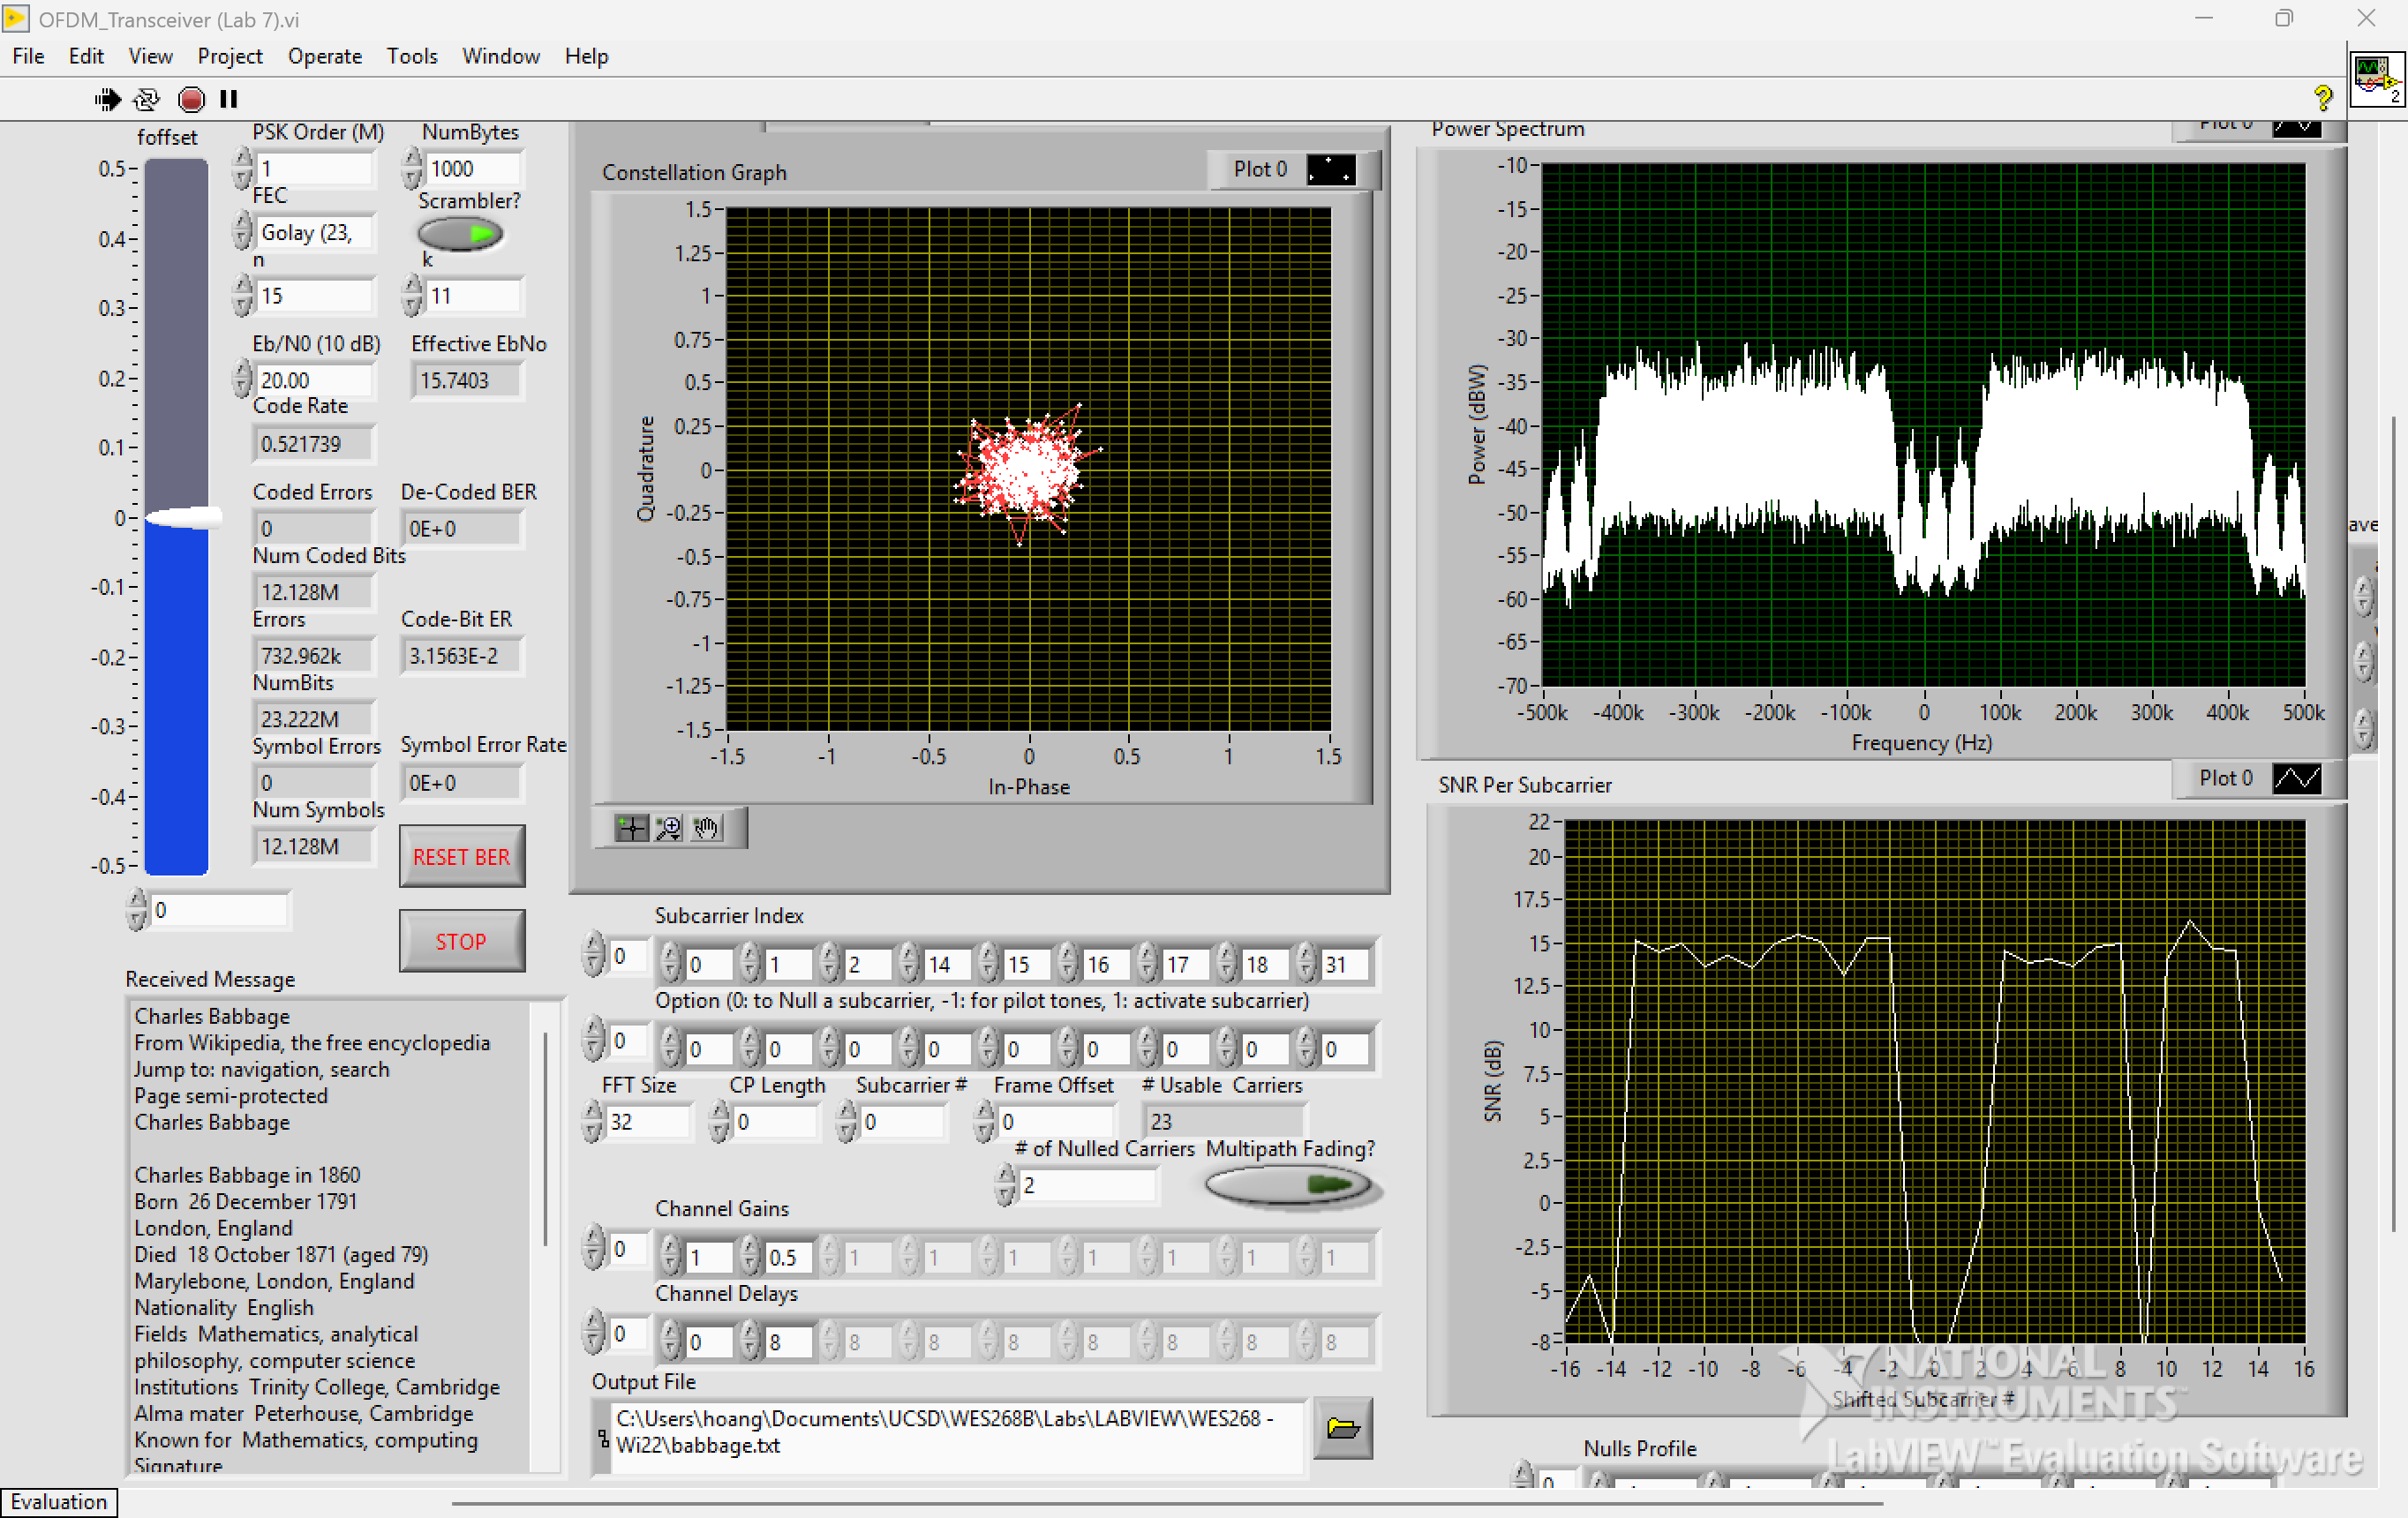
\includegraphics[width=0.7\textwidth]{lab_ss/WES268B_Lab7_Part1-1-7_FEC-Golay23_nullCarriers-2_usableCarriers-23_BER-0.png}
    \caption{Lab 7 - 2 Nulled Subcarriers Golay (23,12) 23 Usable Carriers}
    %\label{f20}
\end{figure}

\begin{figure}[H]
    \centering
    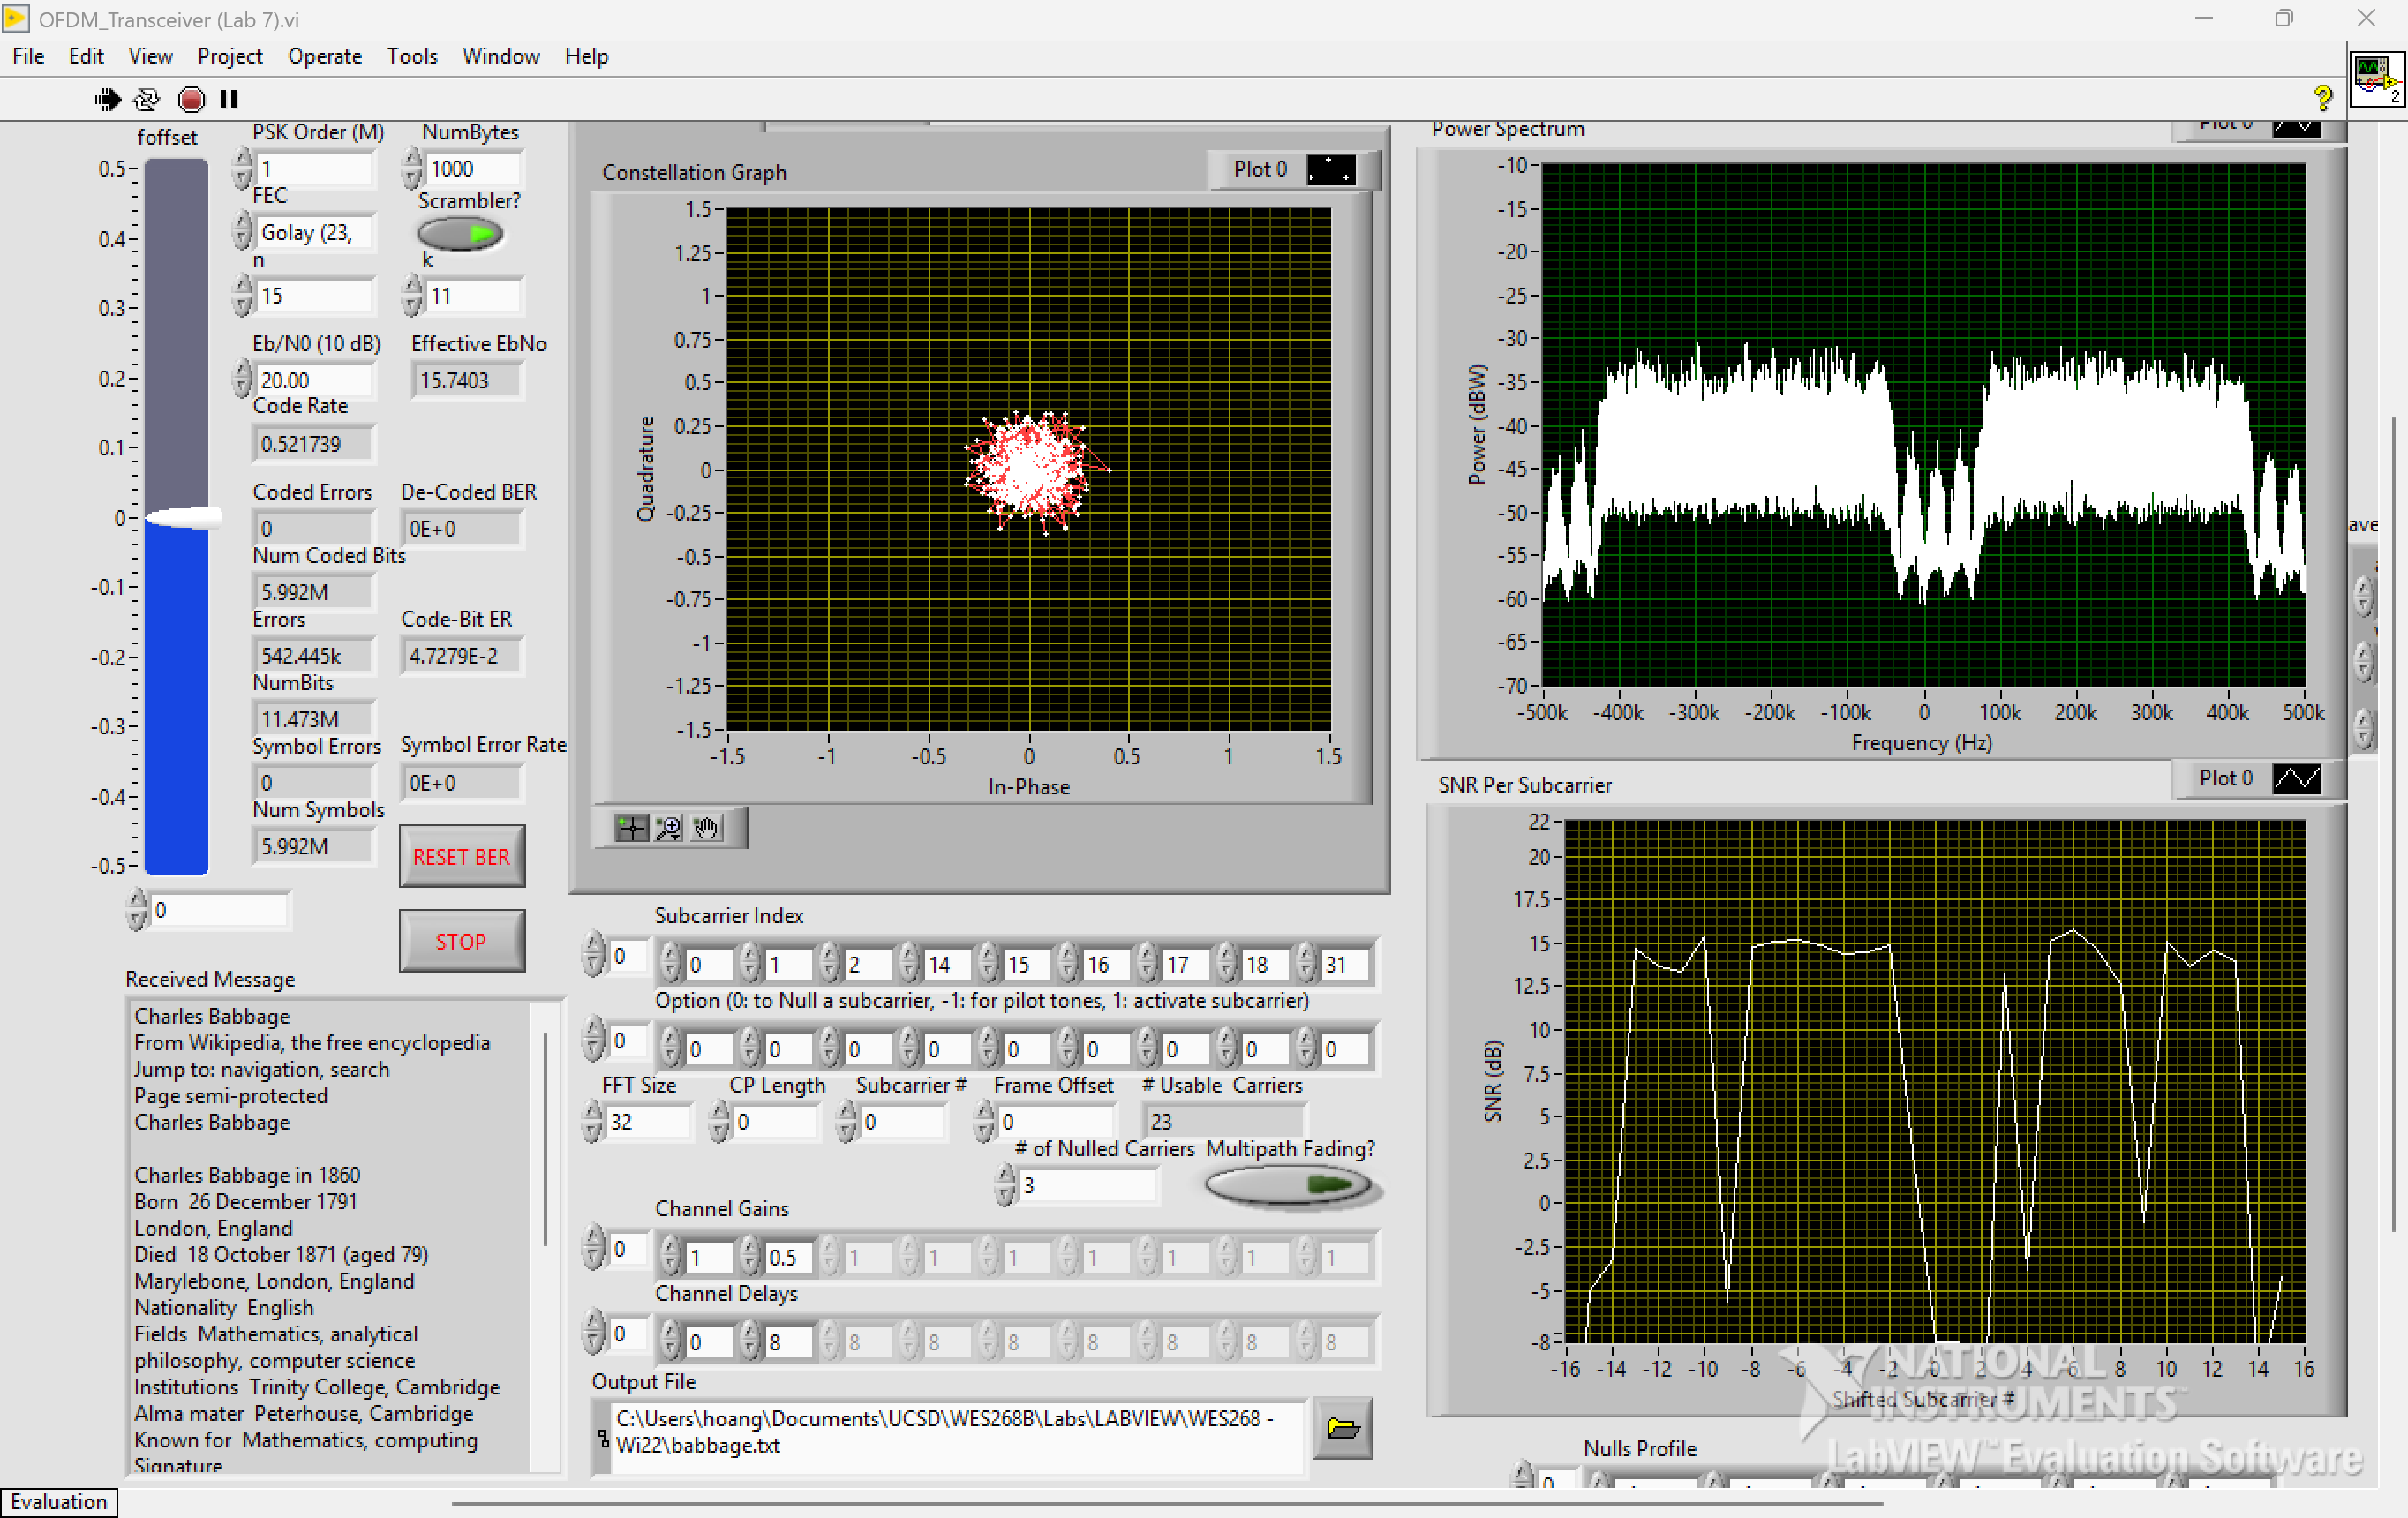
\includegraphics[width=0.7\textwidth]{lab_ss/WES268B_Lab7_Part1-1-7_FEC-Golay23_nullCarriers-3_usableCarriers-23_BER-0.png}
    \caption{Lab 7 - 3 Nulled Subcarriers Golay (23,12) 23 Usable Carriers}
    %\label{f21}
\end{figure}

\begin{figure}[H]
    \centering
    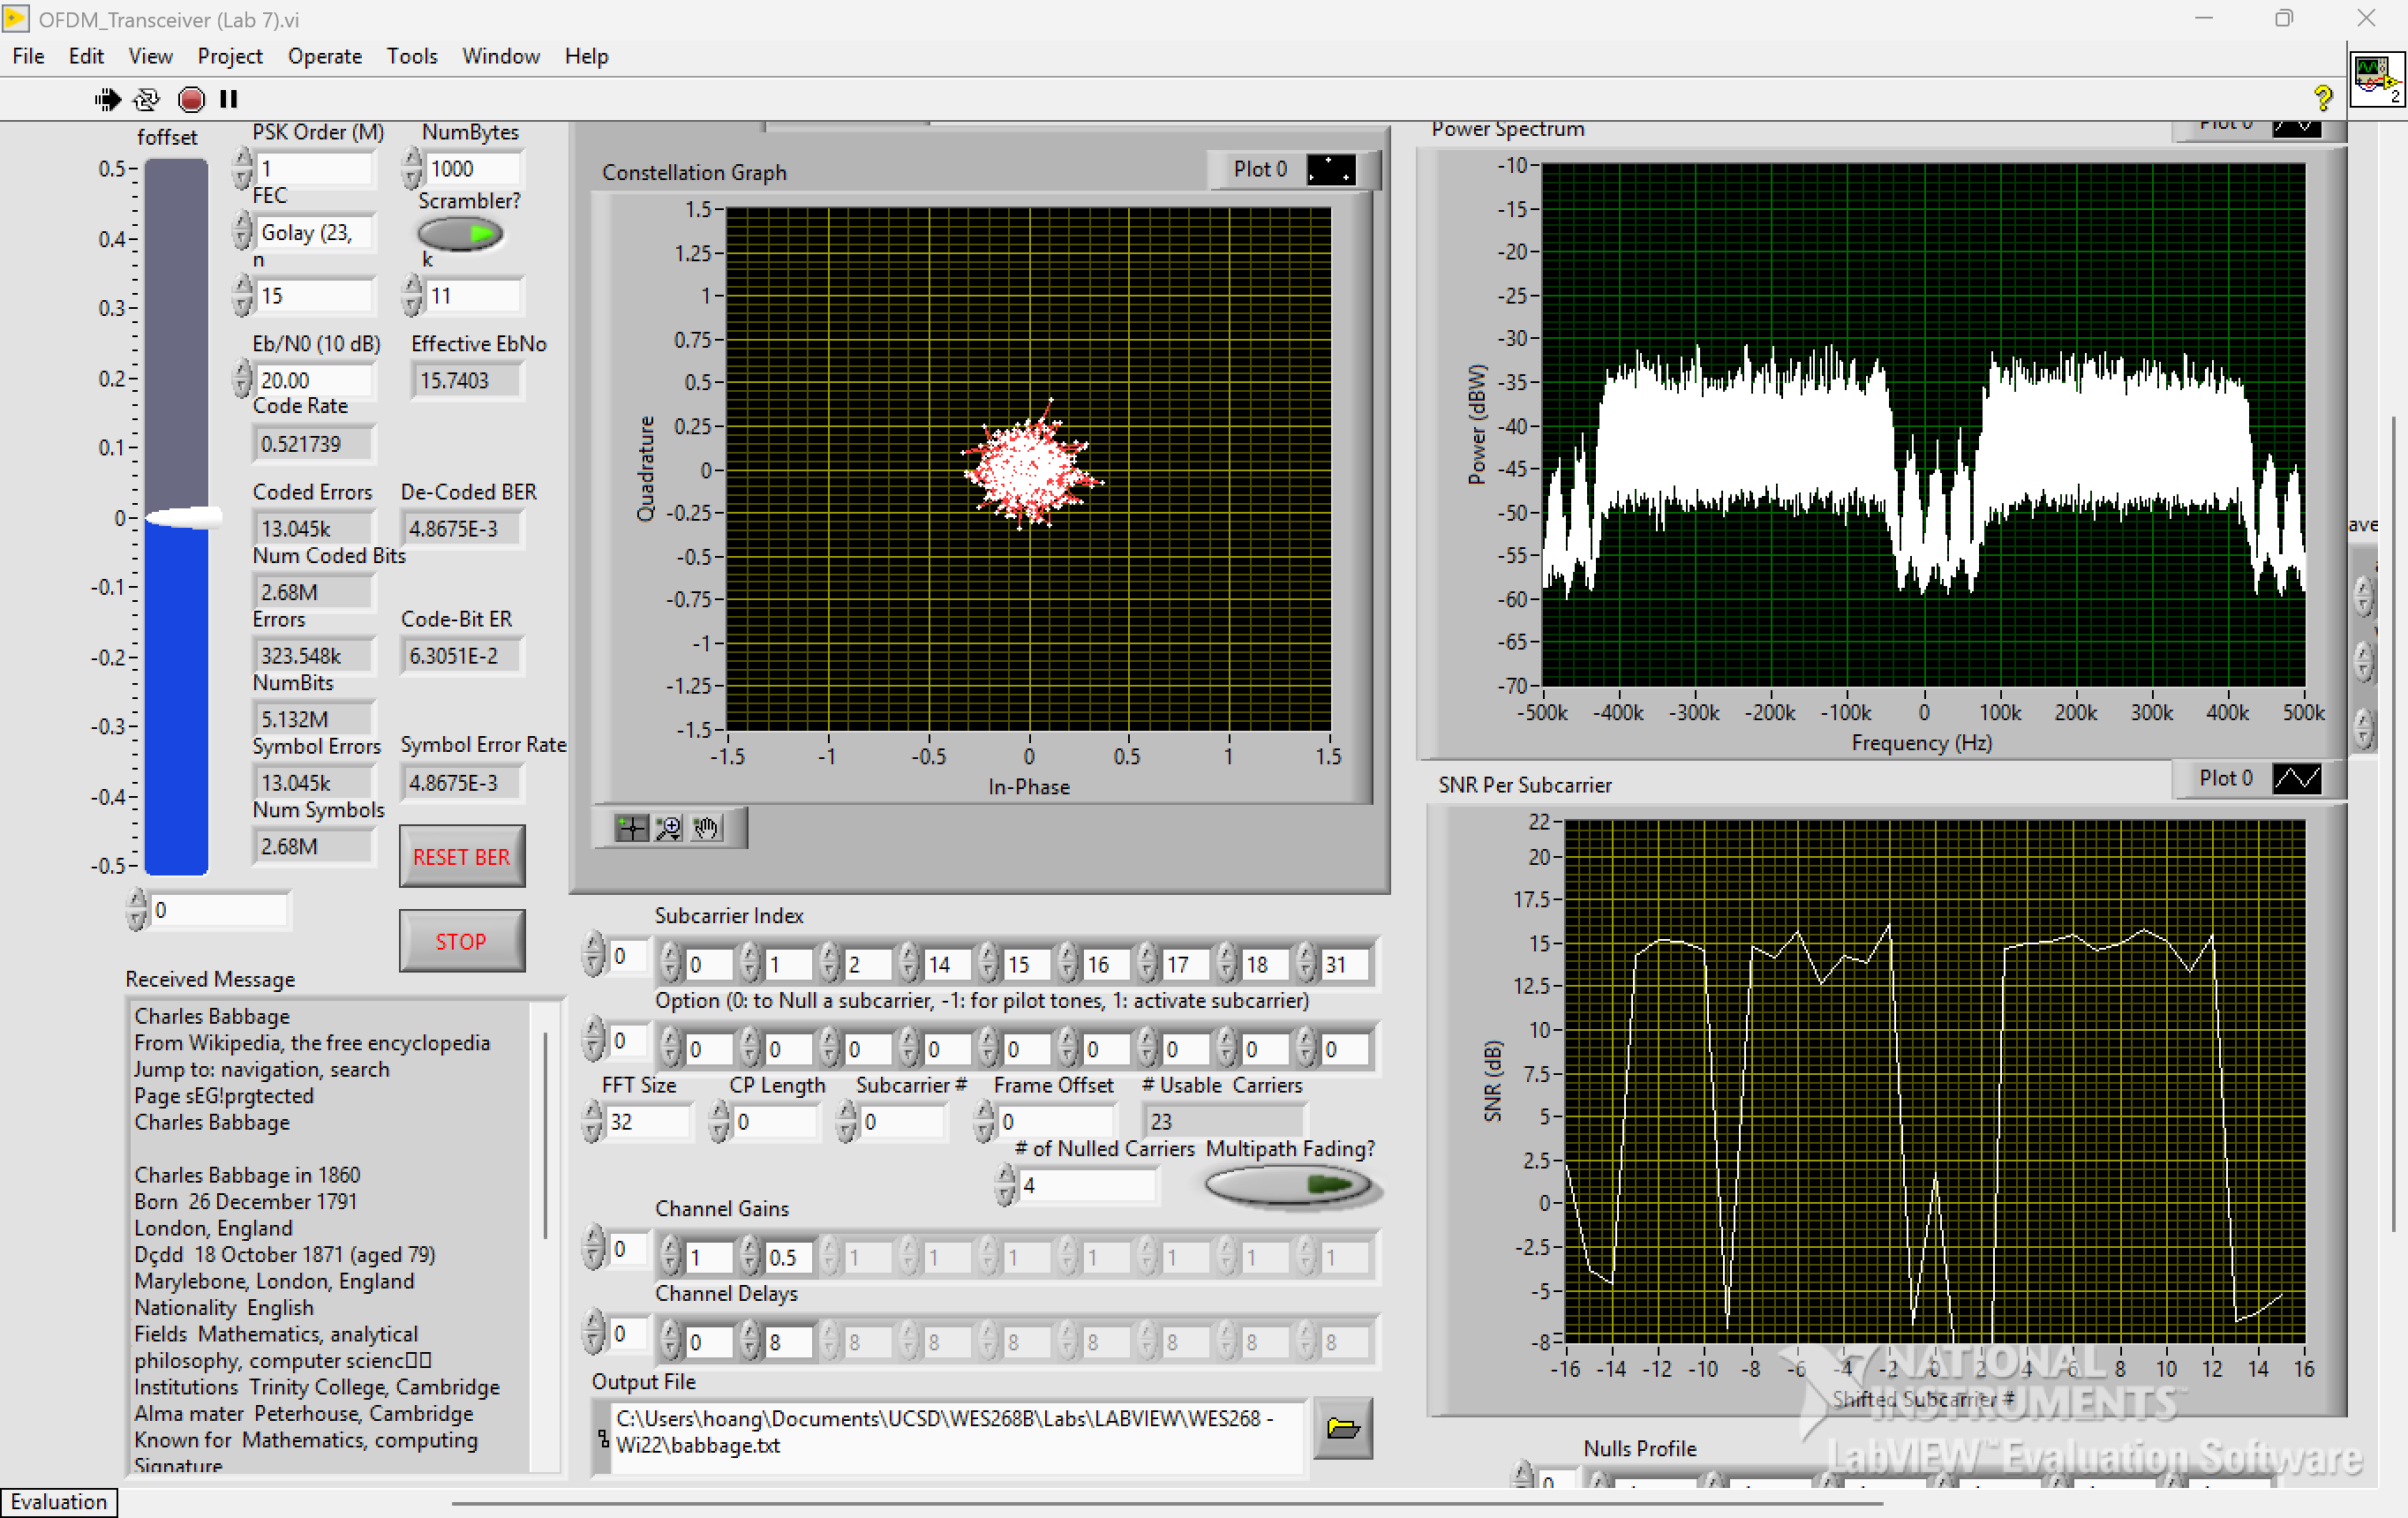
\includegraphics[width=0.7\textwidth]{lab_ss/WES268B_Lab7_Part1-1-7_FEC-Golay23_nullCarriers-4_usableCarriers-23.png}
    \caption{Lab 7 - 4 Nulled Subcarriers Golay (23,12) 23 Usable Carriers}
    %\label{f22_1}
\end{figure}

\begin{figure}[H]
    \centering
    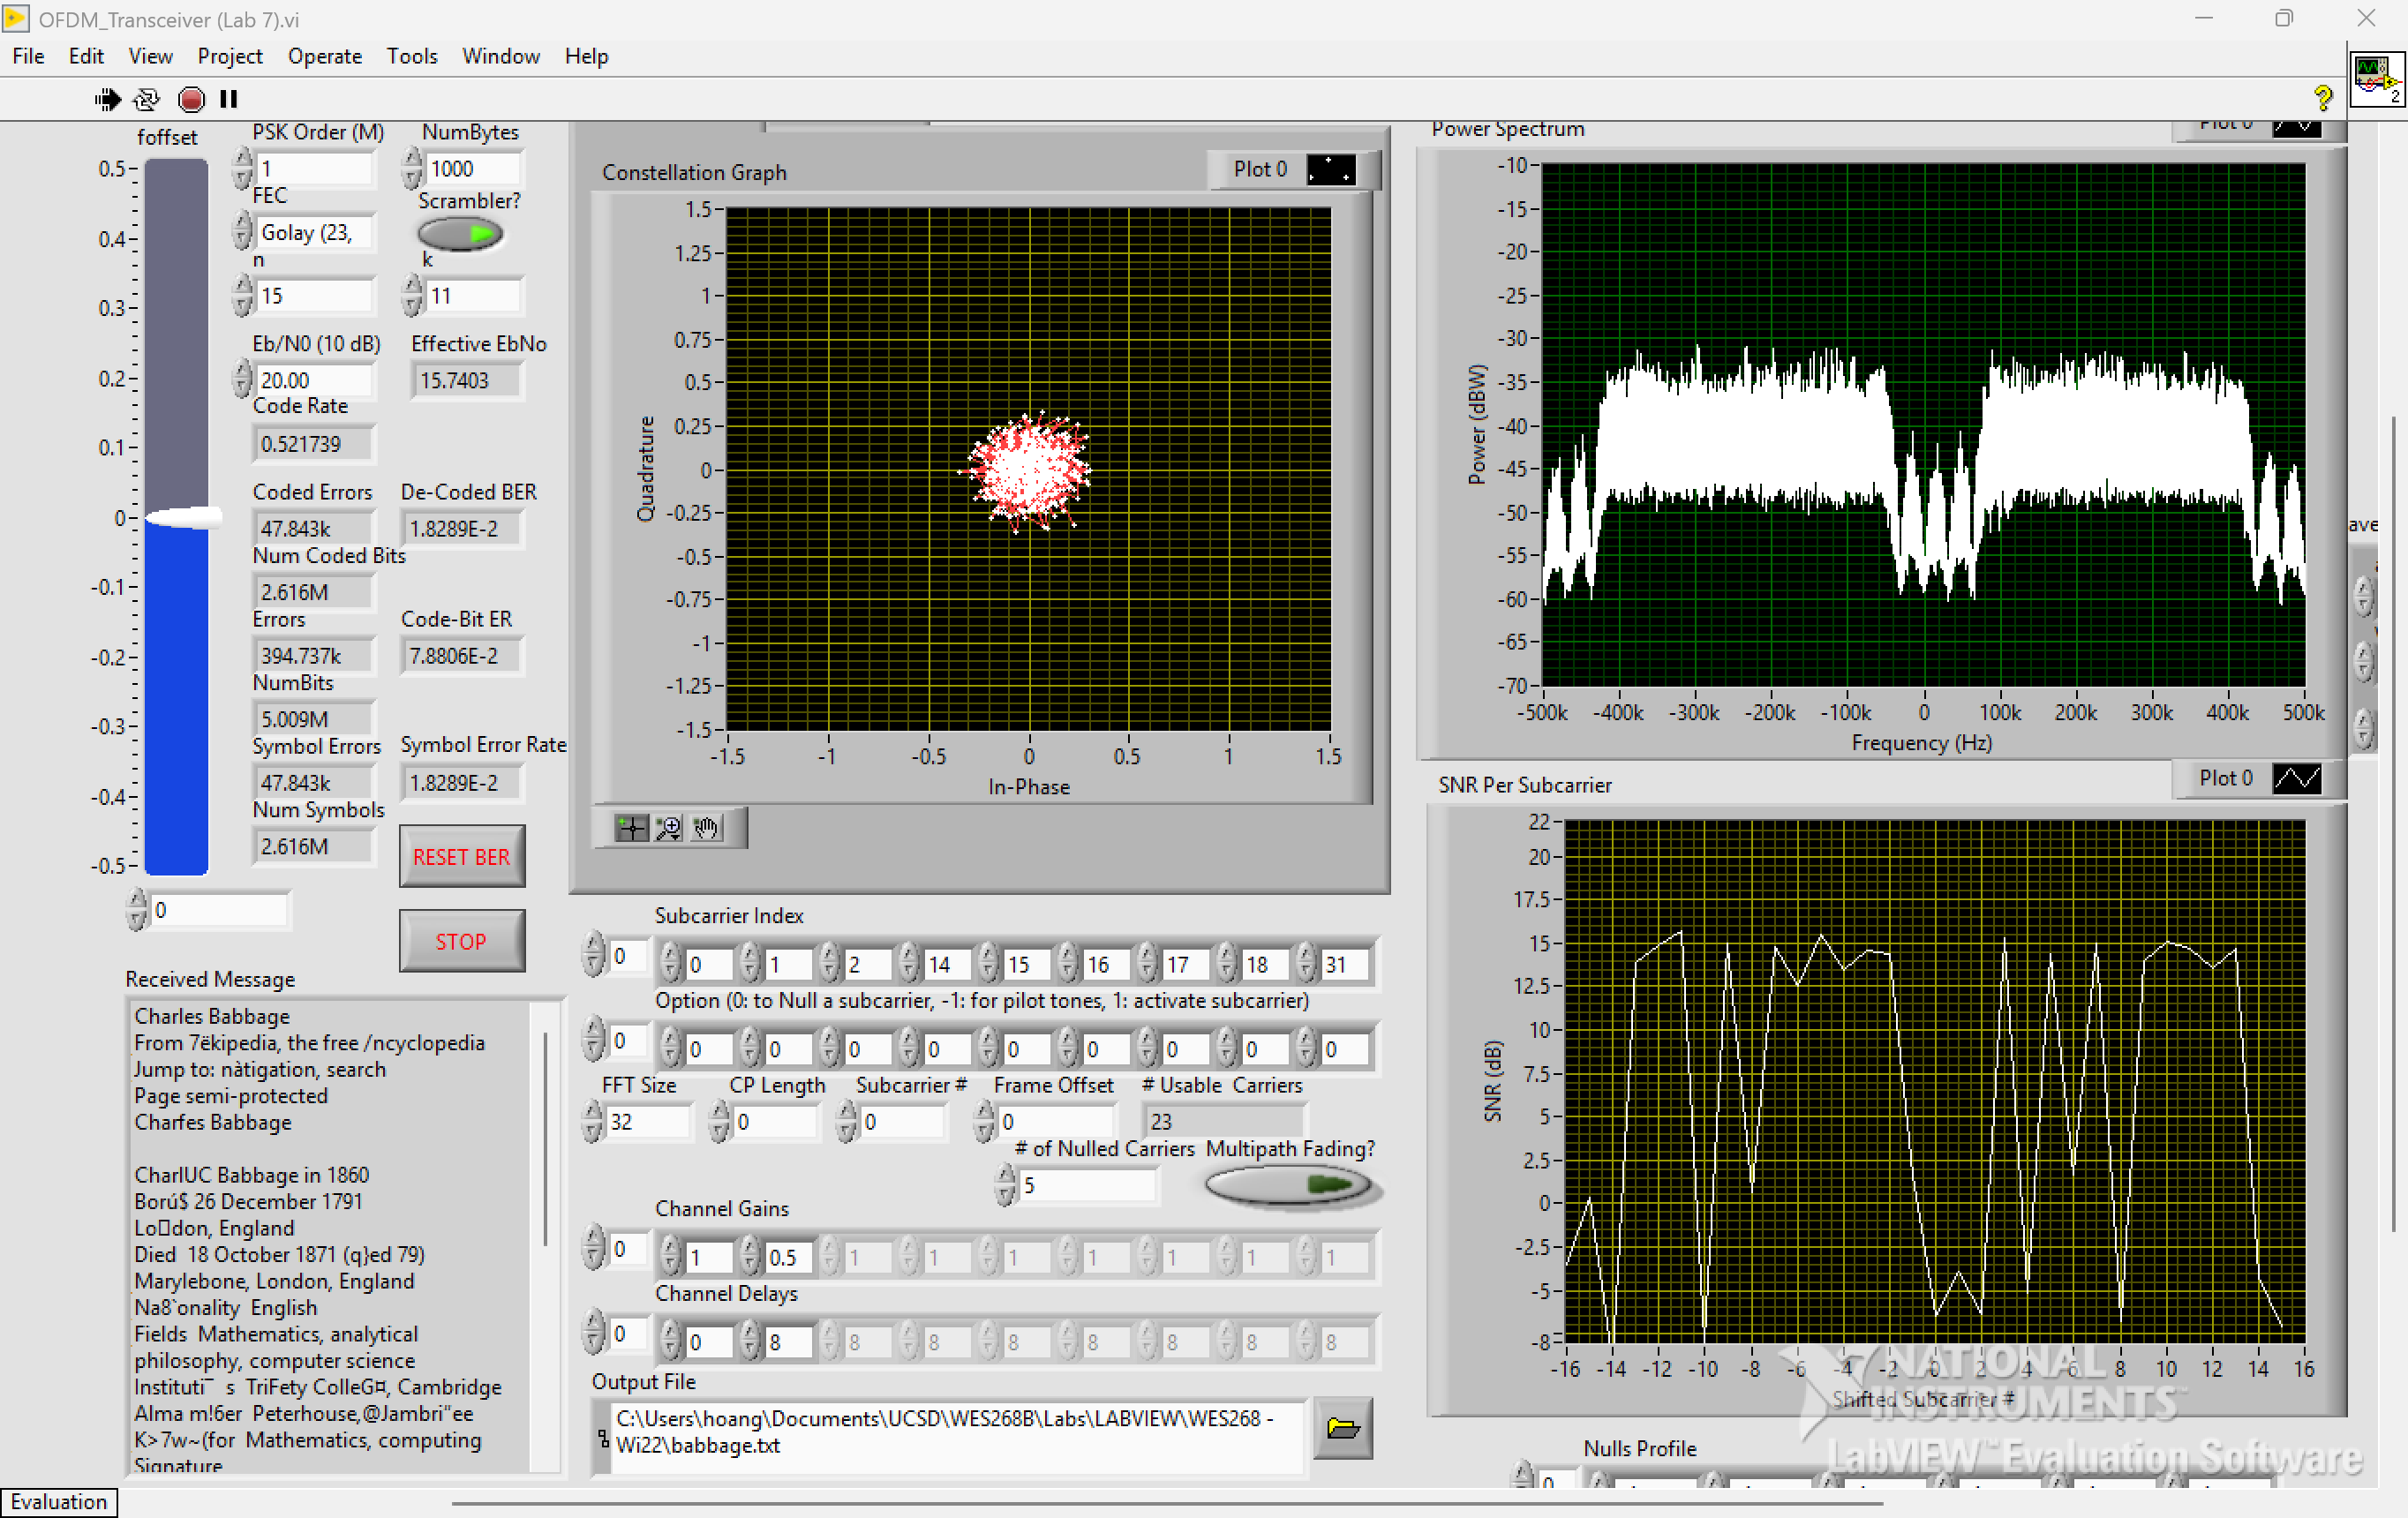
\includegraphics[width=0.7\textwidth]{lab_ss/WES268B_Lab7_Part1-1-7_FEC-Golay23_nullCarriers-5_usableCarriers-23.png}
    \caption{Lab 7 - 5 Nulled Subcarriers Golay (23,12) 23 Usable Carriers}
    %\label{f23_1}
\end{figure}

\begin{figure}[H]
    \centering
    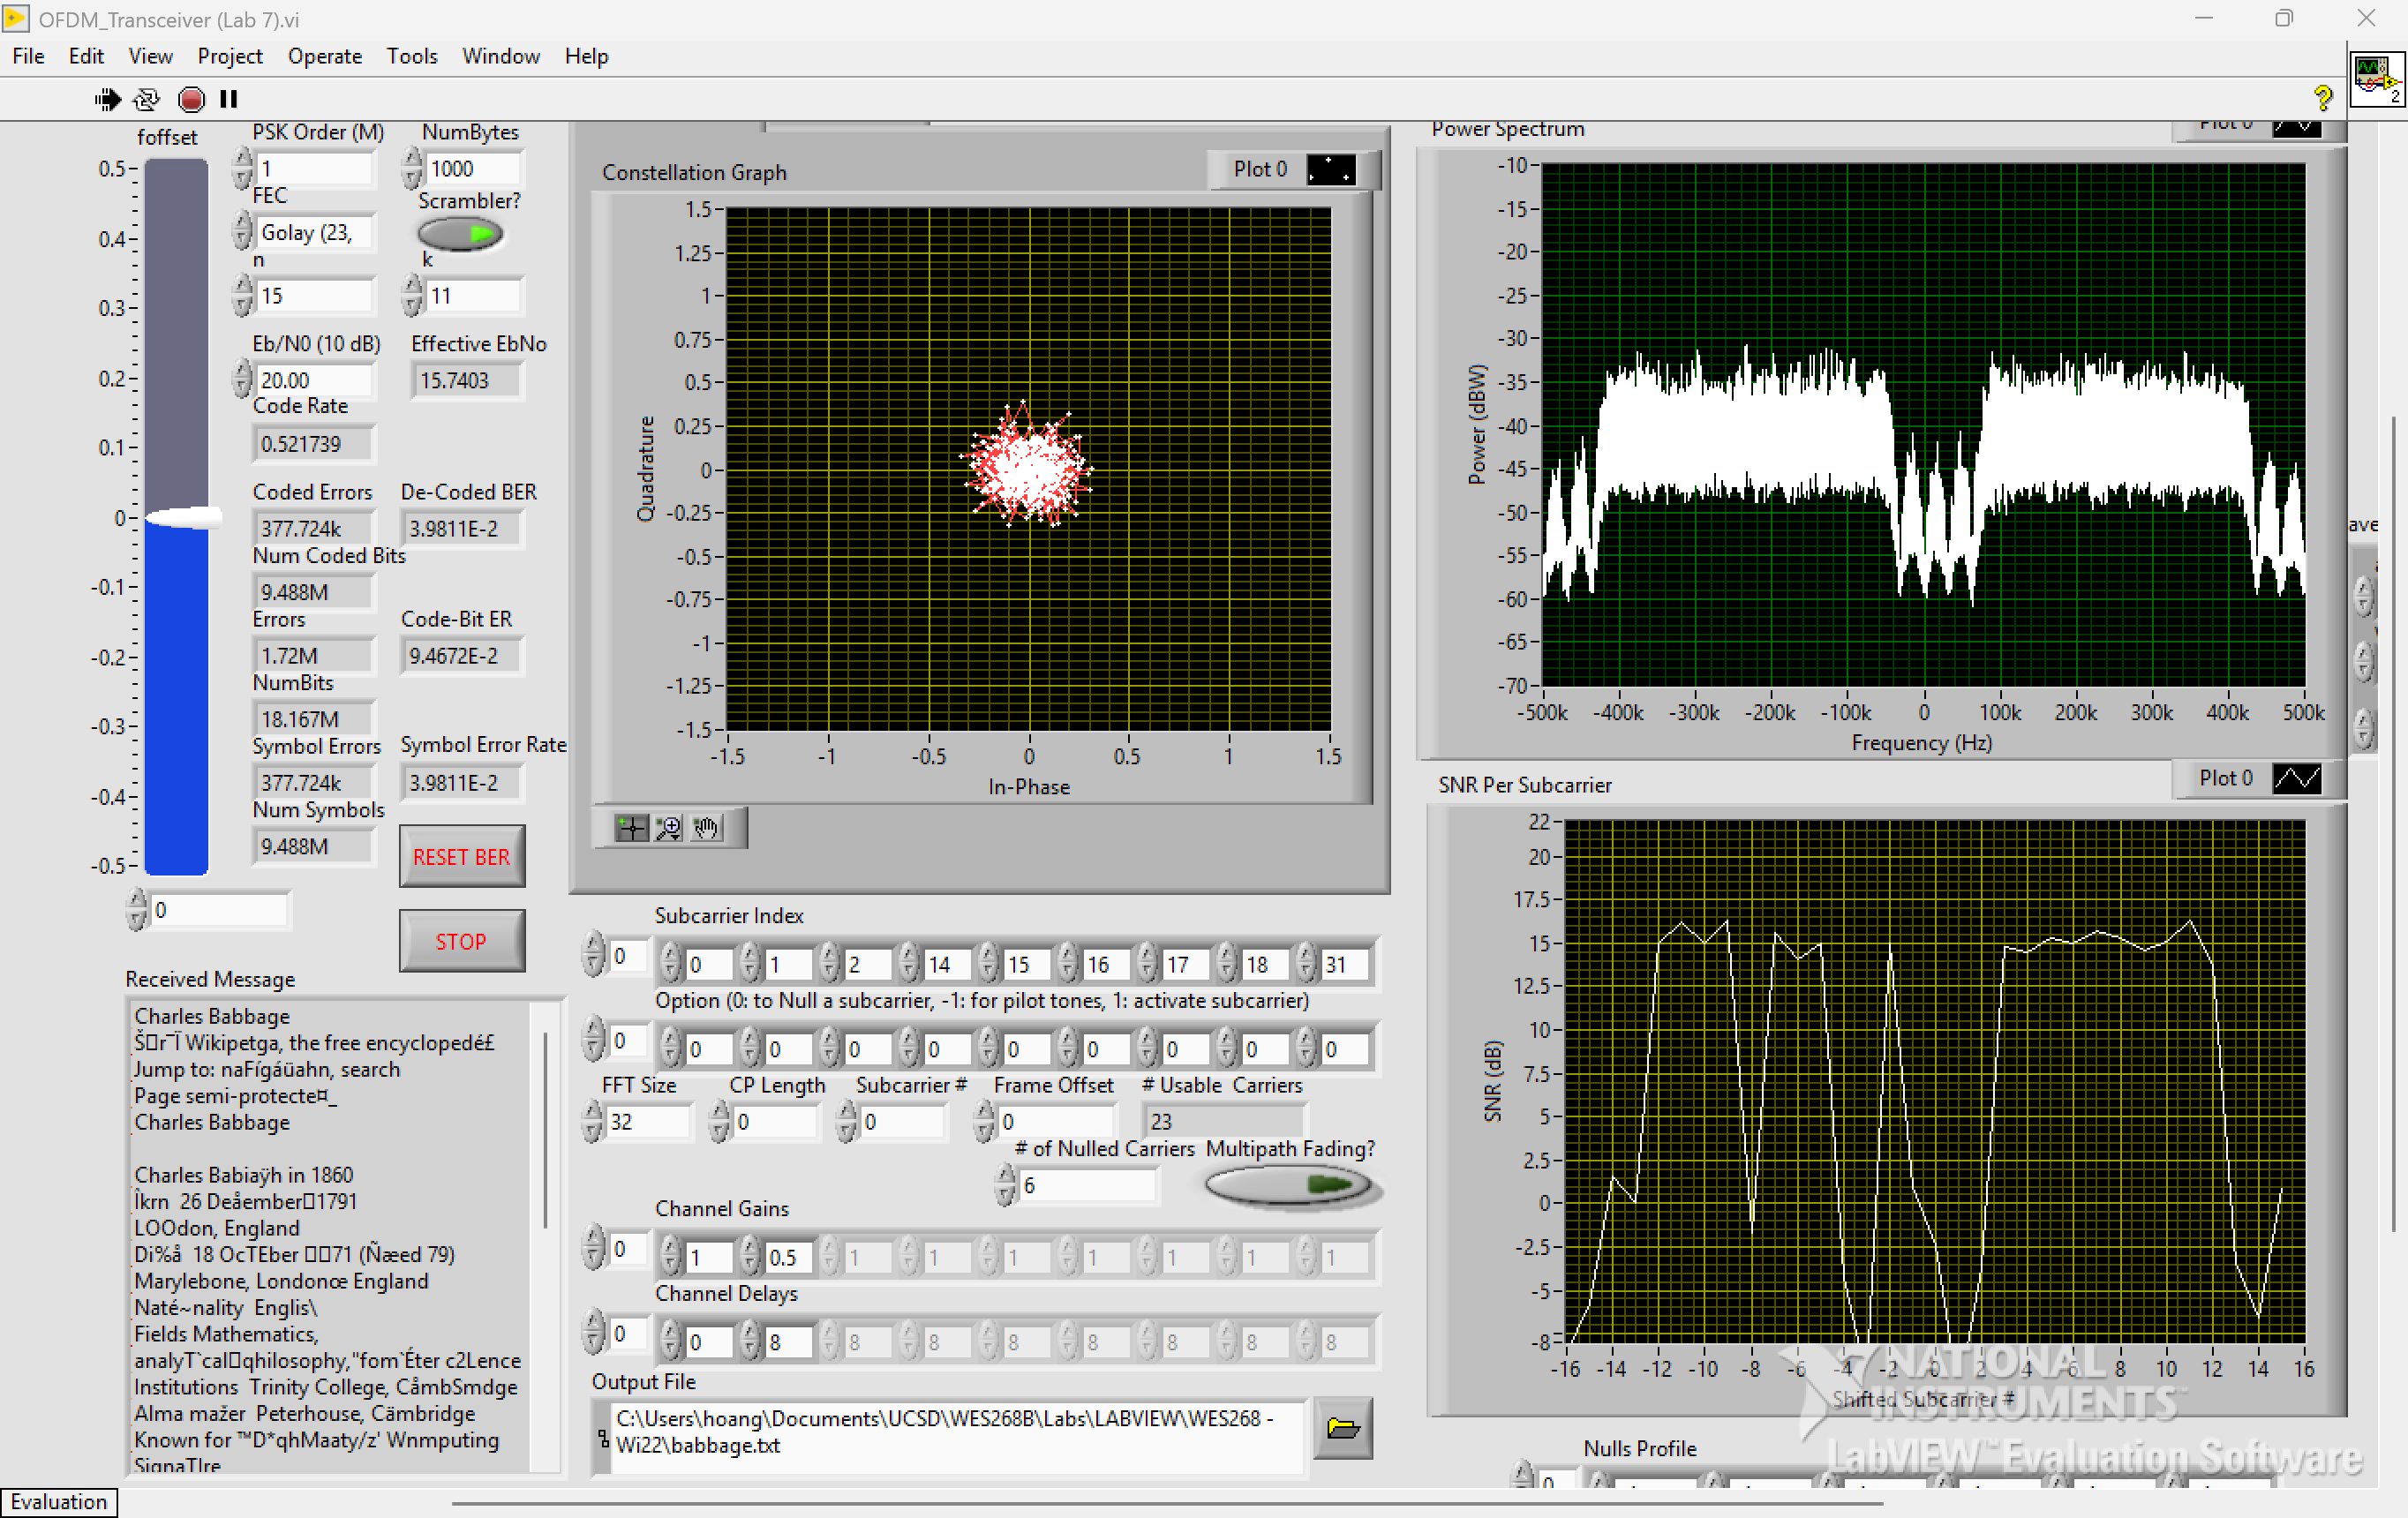
\includegraphics[width=0.7\textwidth]{lab_ss/WES268B_Lab7_Part1-1-7_FEC-Golay23_nullCarriers-6_usableCarriers-23.png}
    \caption{Lab 7 - 6 Nulled Subcarriers Golay (23,12) 23 Usable Carriers}
    %\label{f22_2}
\end{figure}

\subsubsection{ }
\noindent\textbf{Question.} 

\noindent\textbf{Answer.} 
{
    Based on our results, the (23,12) Golay code performed better than the (24,12) Golay code. At first, this was unexpected because 
    the extra bit increases our minimum distance from 7 to 8 which should improve our error correcting capability. But with a (23,12) setup,
    the codeword fits into one OFDM symbol. With a (24,12) setup, the codeword is spread across two symbols so some symbols will see 0 erasures and 
    some symbols will see 2 erasures. This might cause our overall error to be spread less evenly, leading to a higher decoded BER than our (23,12) setup.
}

% 2 Peak to Average Power Ratio (PAPR)
\section{Peak to Average Power Ratio (PAPR)}

% 2.1
\subsection{Scrambling}

% 2.1.1
\subsubsection{}
% 2.1.2
\subsubsection{}
\begin{figure}[H]
    \centering
    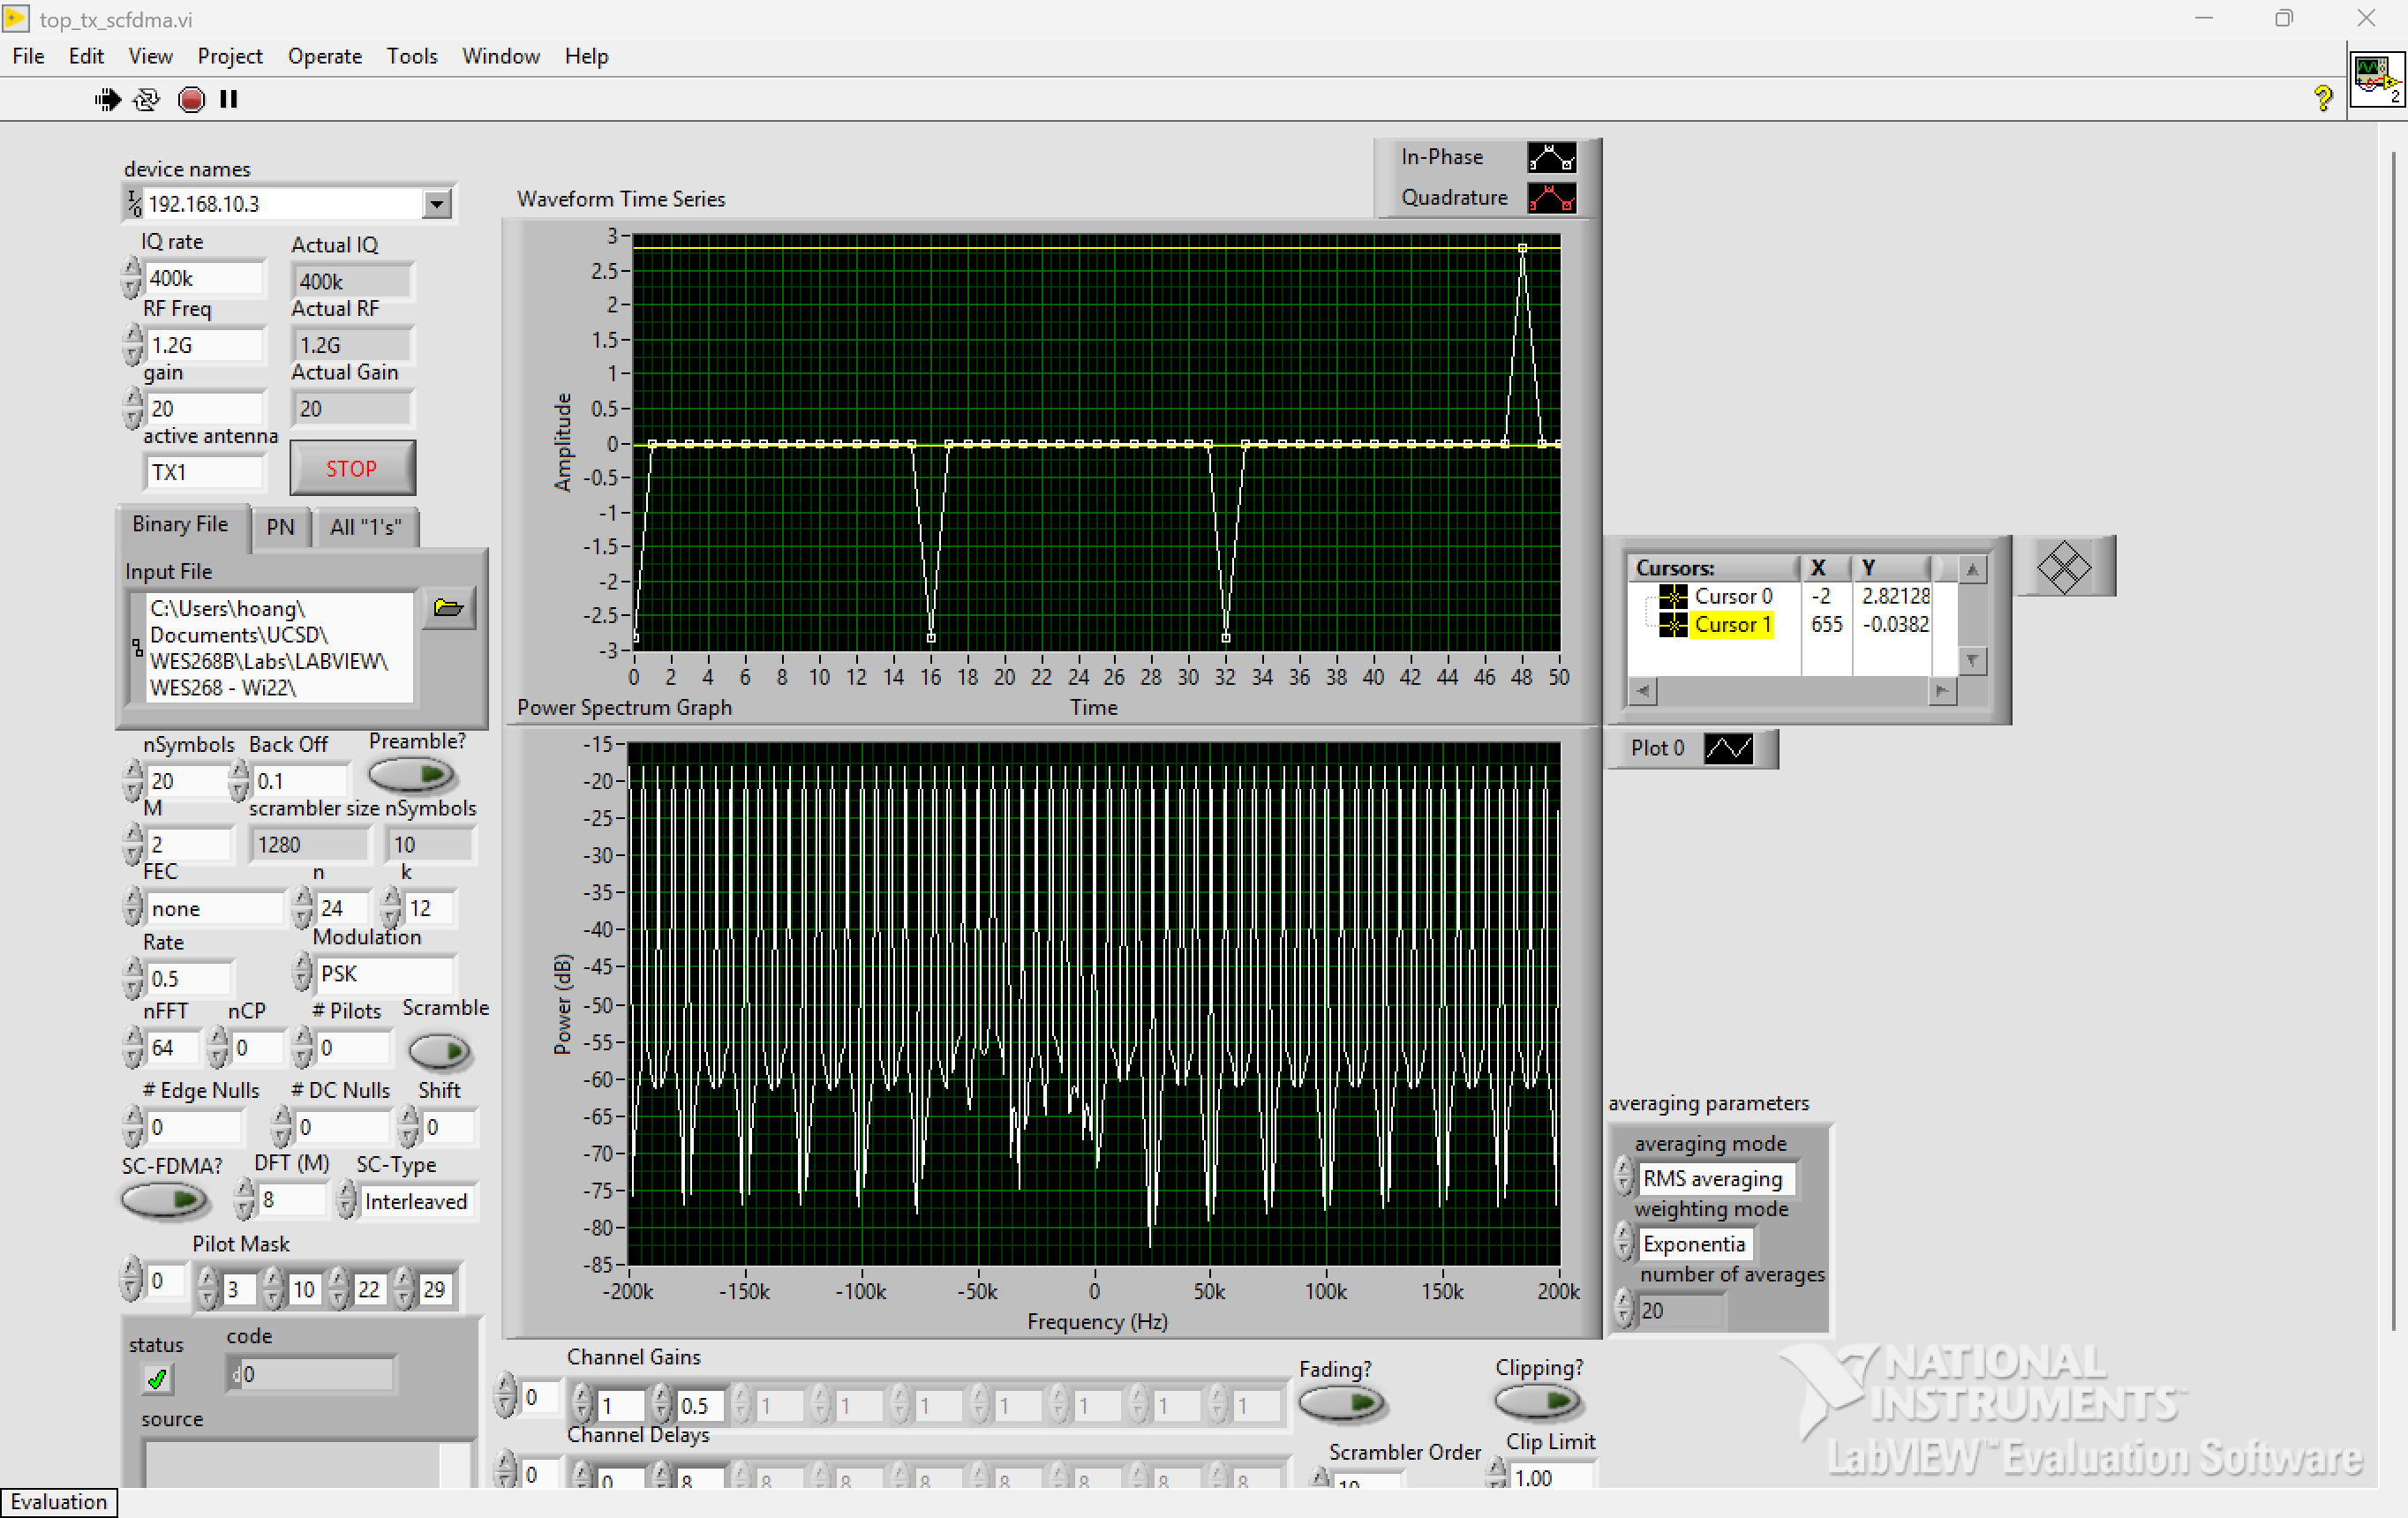
\includegraphics[width=0.7\textwidth]{lab_ss/WES268B_Lab7_Part2-1-2a_scramblerOFF_nFFT-64_PAPR-12dB_idk.png}
    \caption{Lab 7 - Scrambler OFF, Uncompressed File Input, FFT Size = 64, PAPR = 12dB}
    %\label{f23_2}
\end{figure}

\begin{figure}[H]
    \centering
    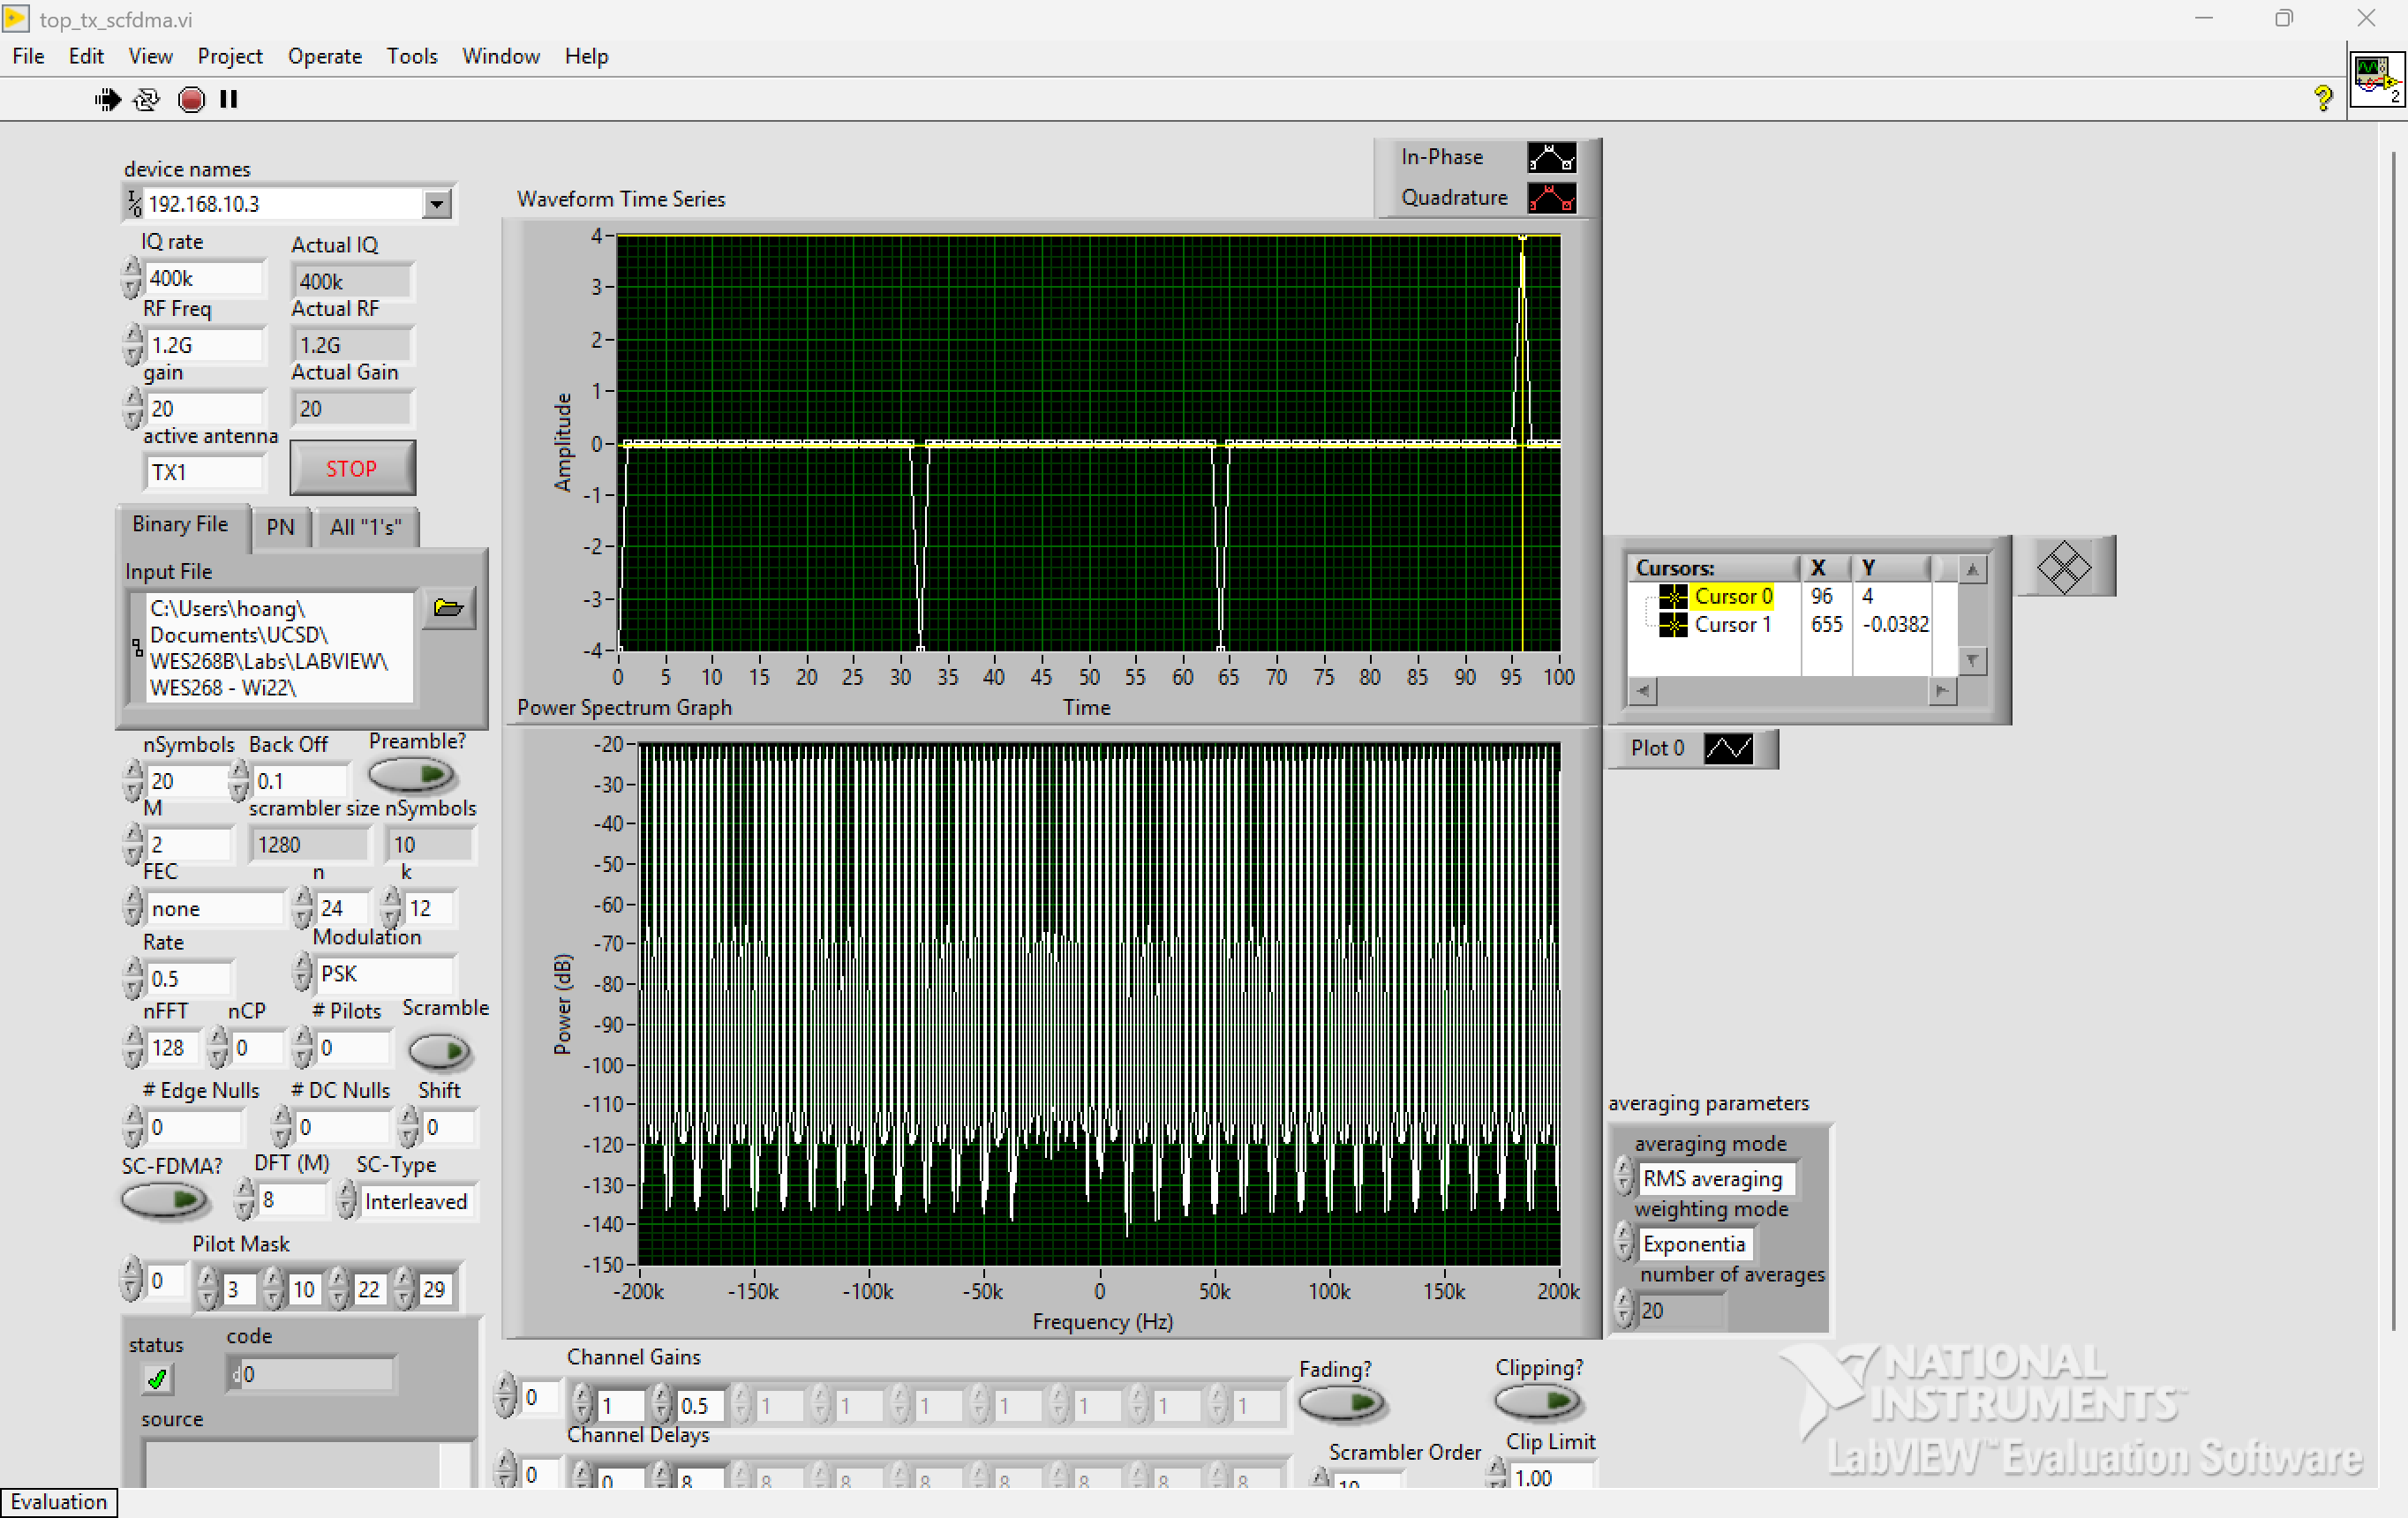
\includegraphics[width=0.7\textwidth]{lab_ss/WES268B_Lab7_Part2-1-2a_scramblerOFF_nFFT-128_PAPR-15dB_idk.png}
    \caption{Lab 7 - Scrambler OFF, Uncompressed File Input, FFT Size = 128, PAPR = 15dB}
    %\label{f24}
\end{figure}

\begin{figure}[H]
    \centering
    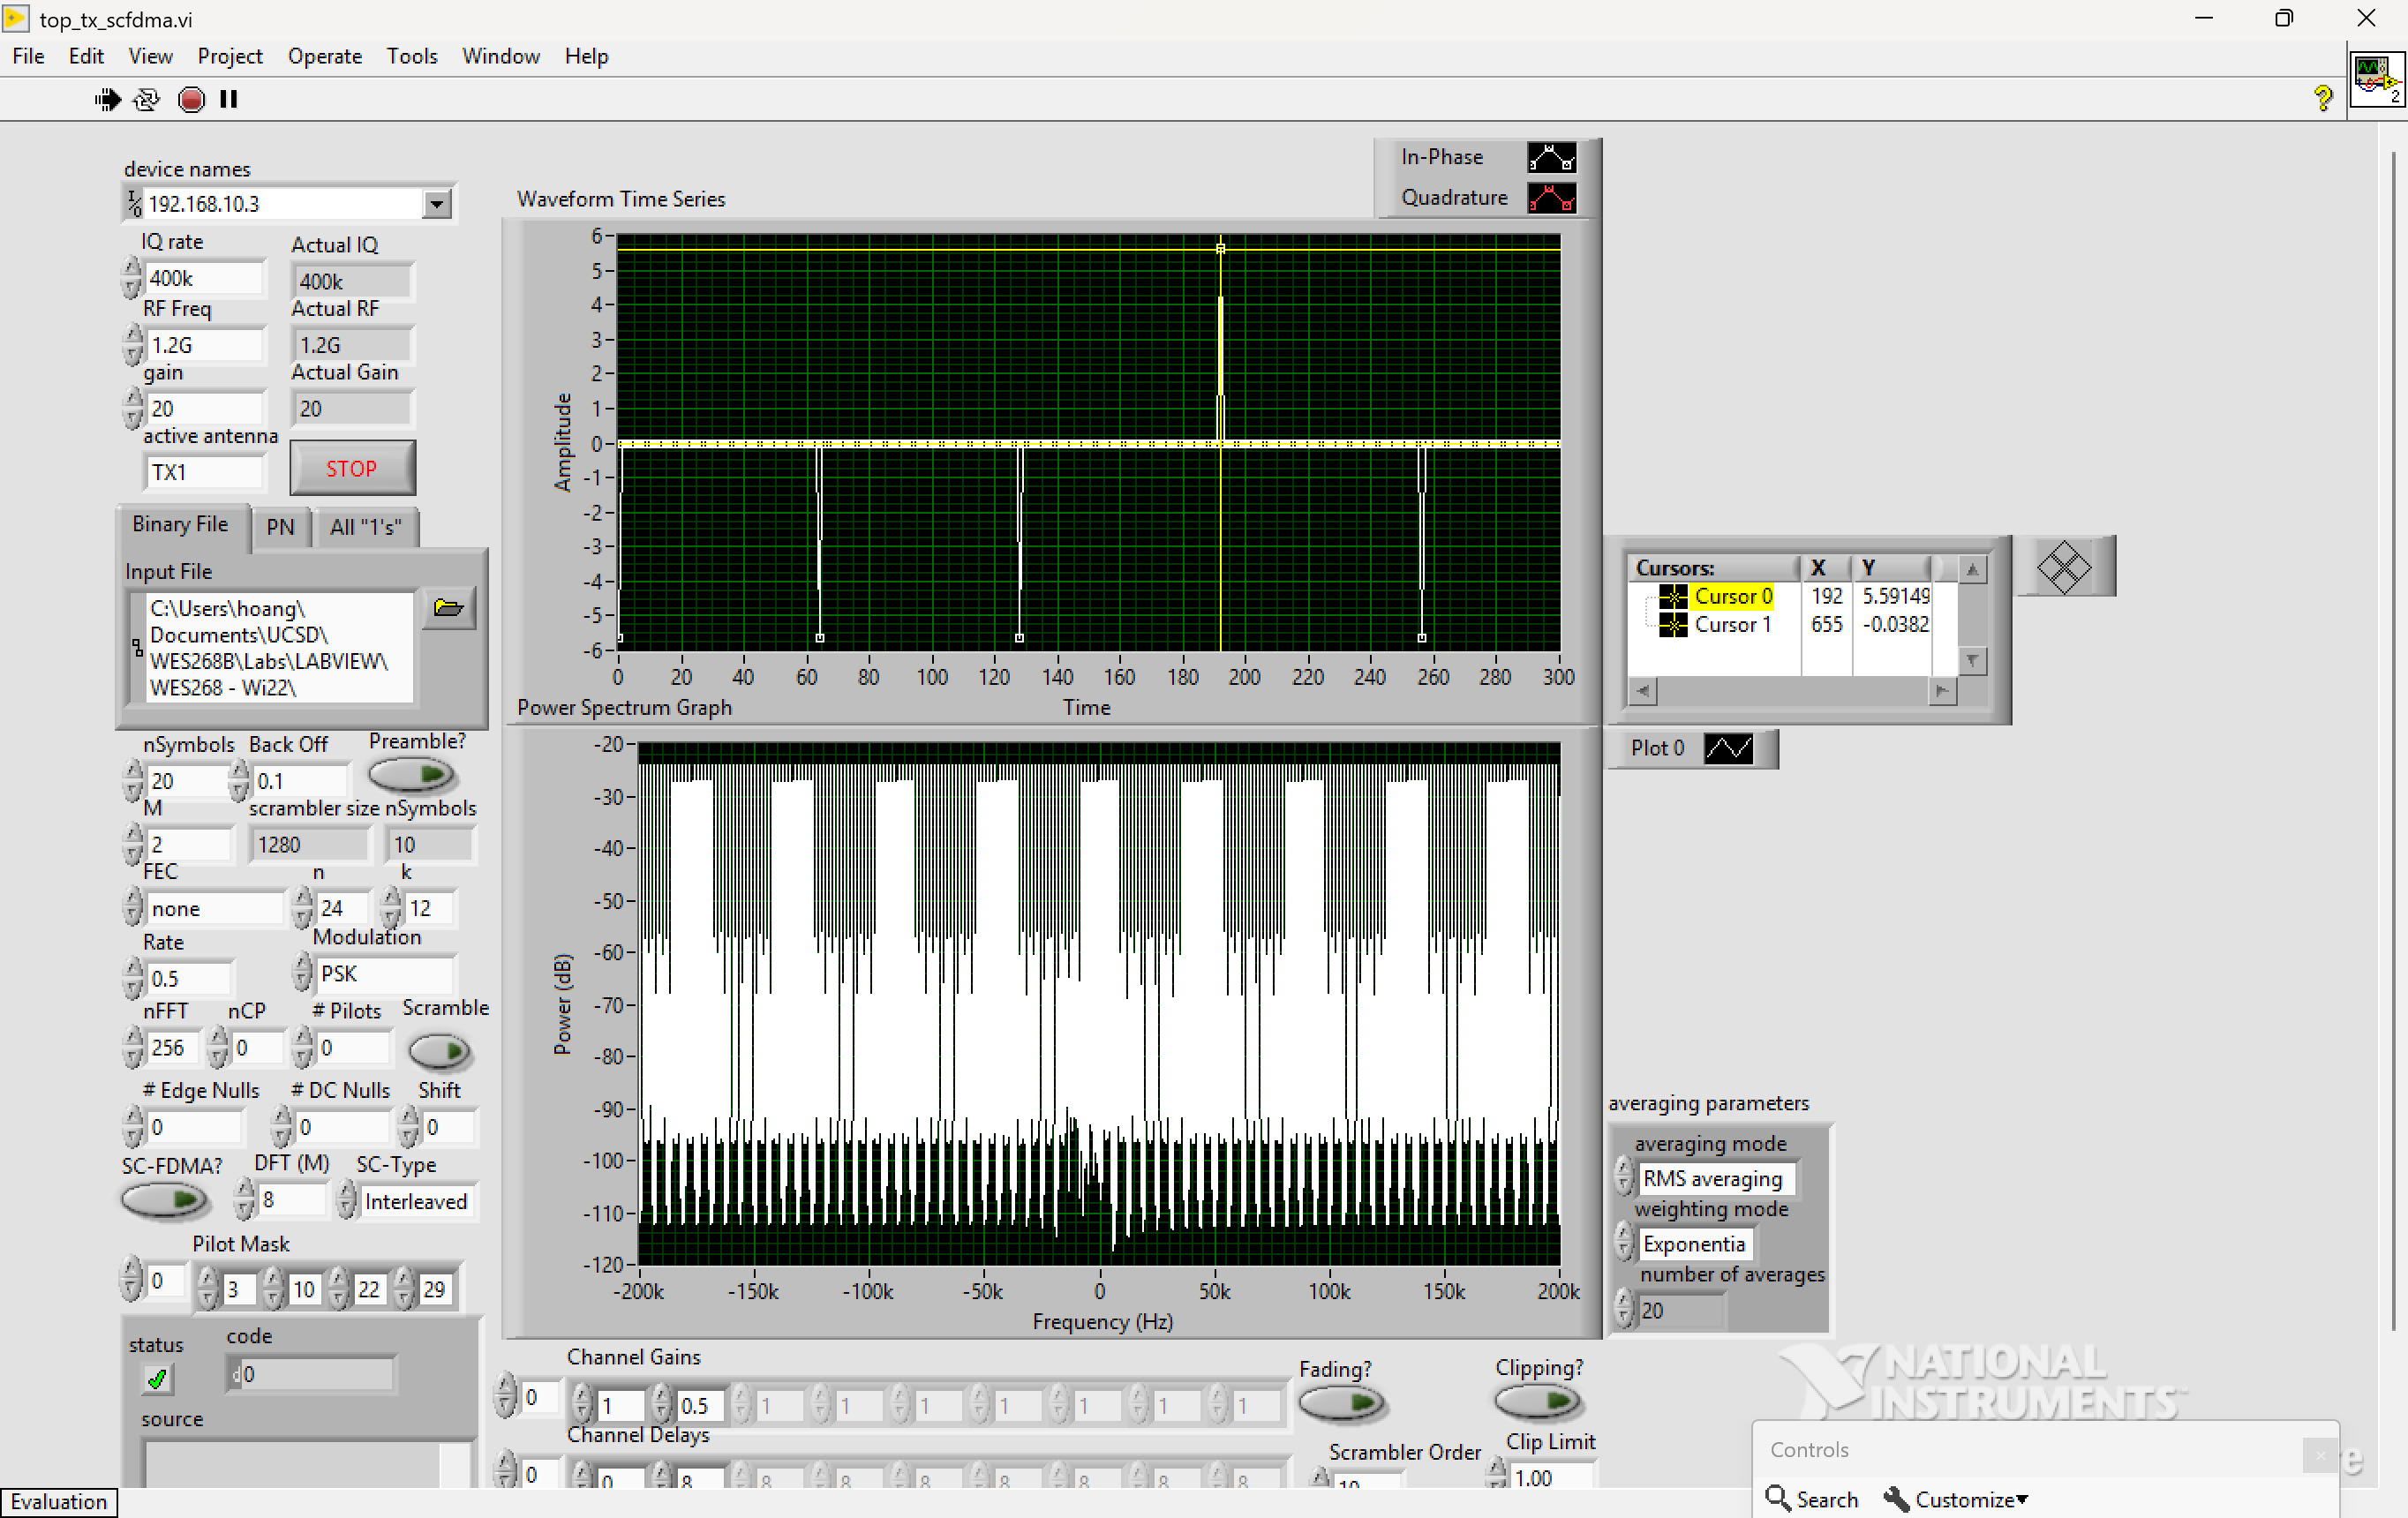
\includegraphics[width=0.7\textwidth]{lab_ss/WES268B_Lab7_Part2-1-2a_scramblerOFF_nFFT-256_PAPR-18dB_idk.png}
    \caption{Lab 7 - Scrambler OFF, Uncompressed File Input, FFT Size = 256, PAPR = 18dB}
    %\label{f25}
\end{figure}

\begin{figure}[H]
    \centering
    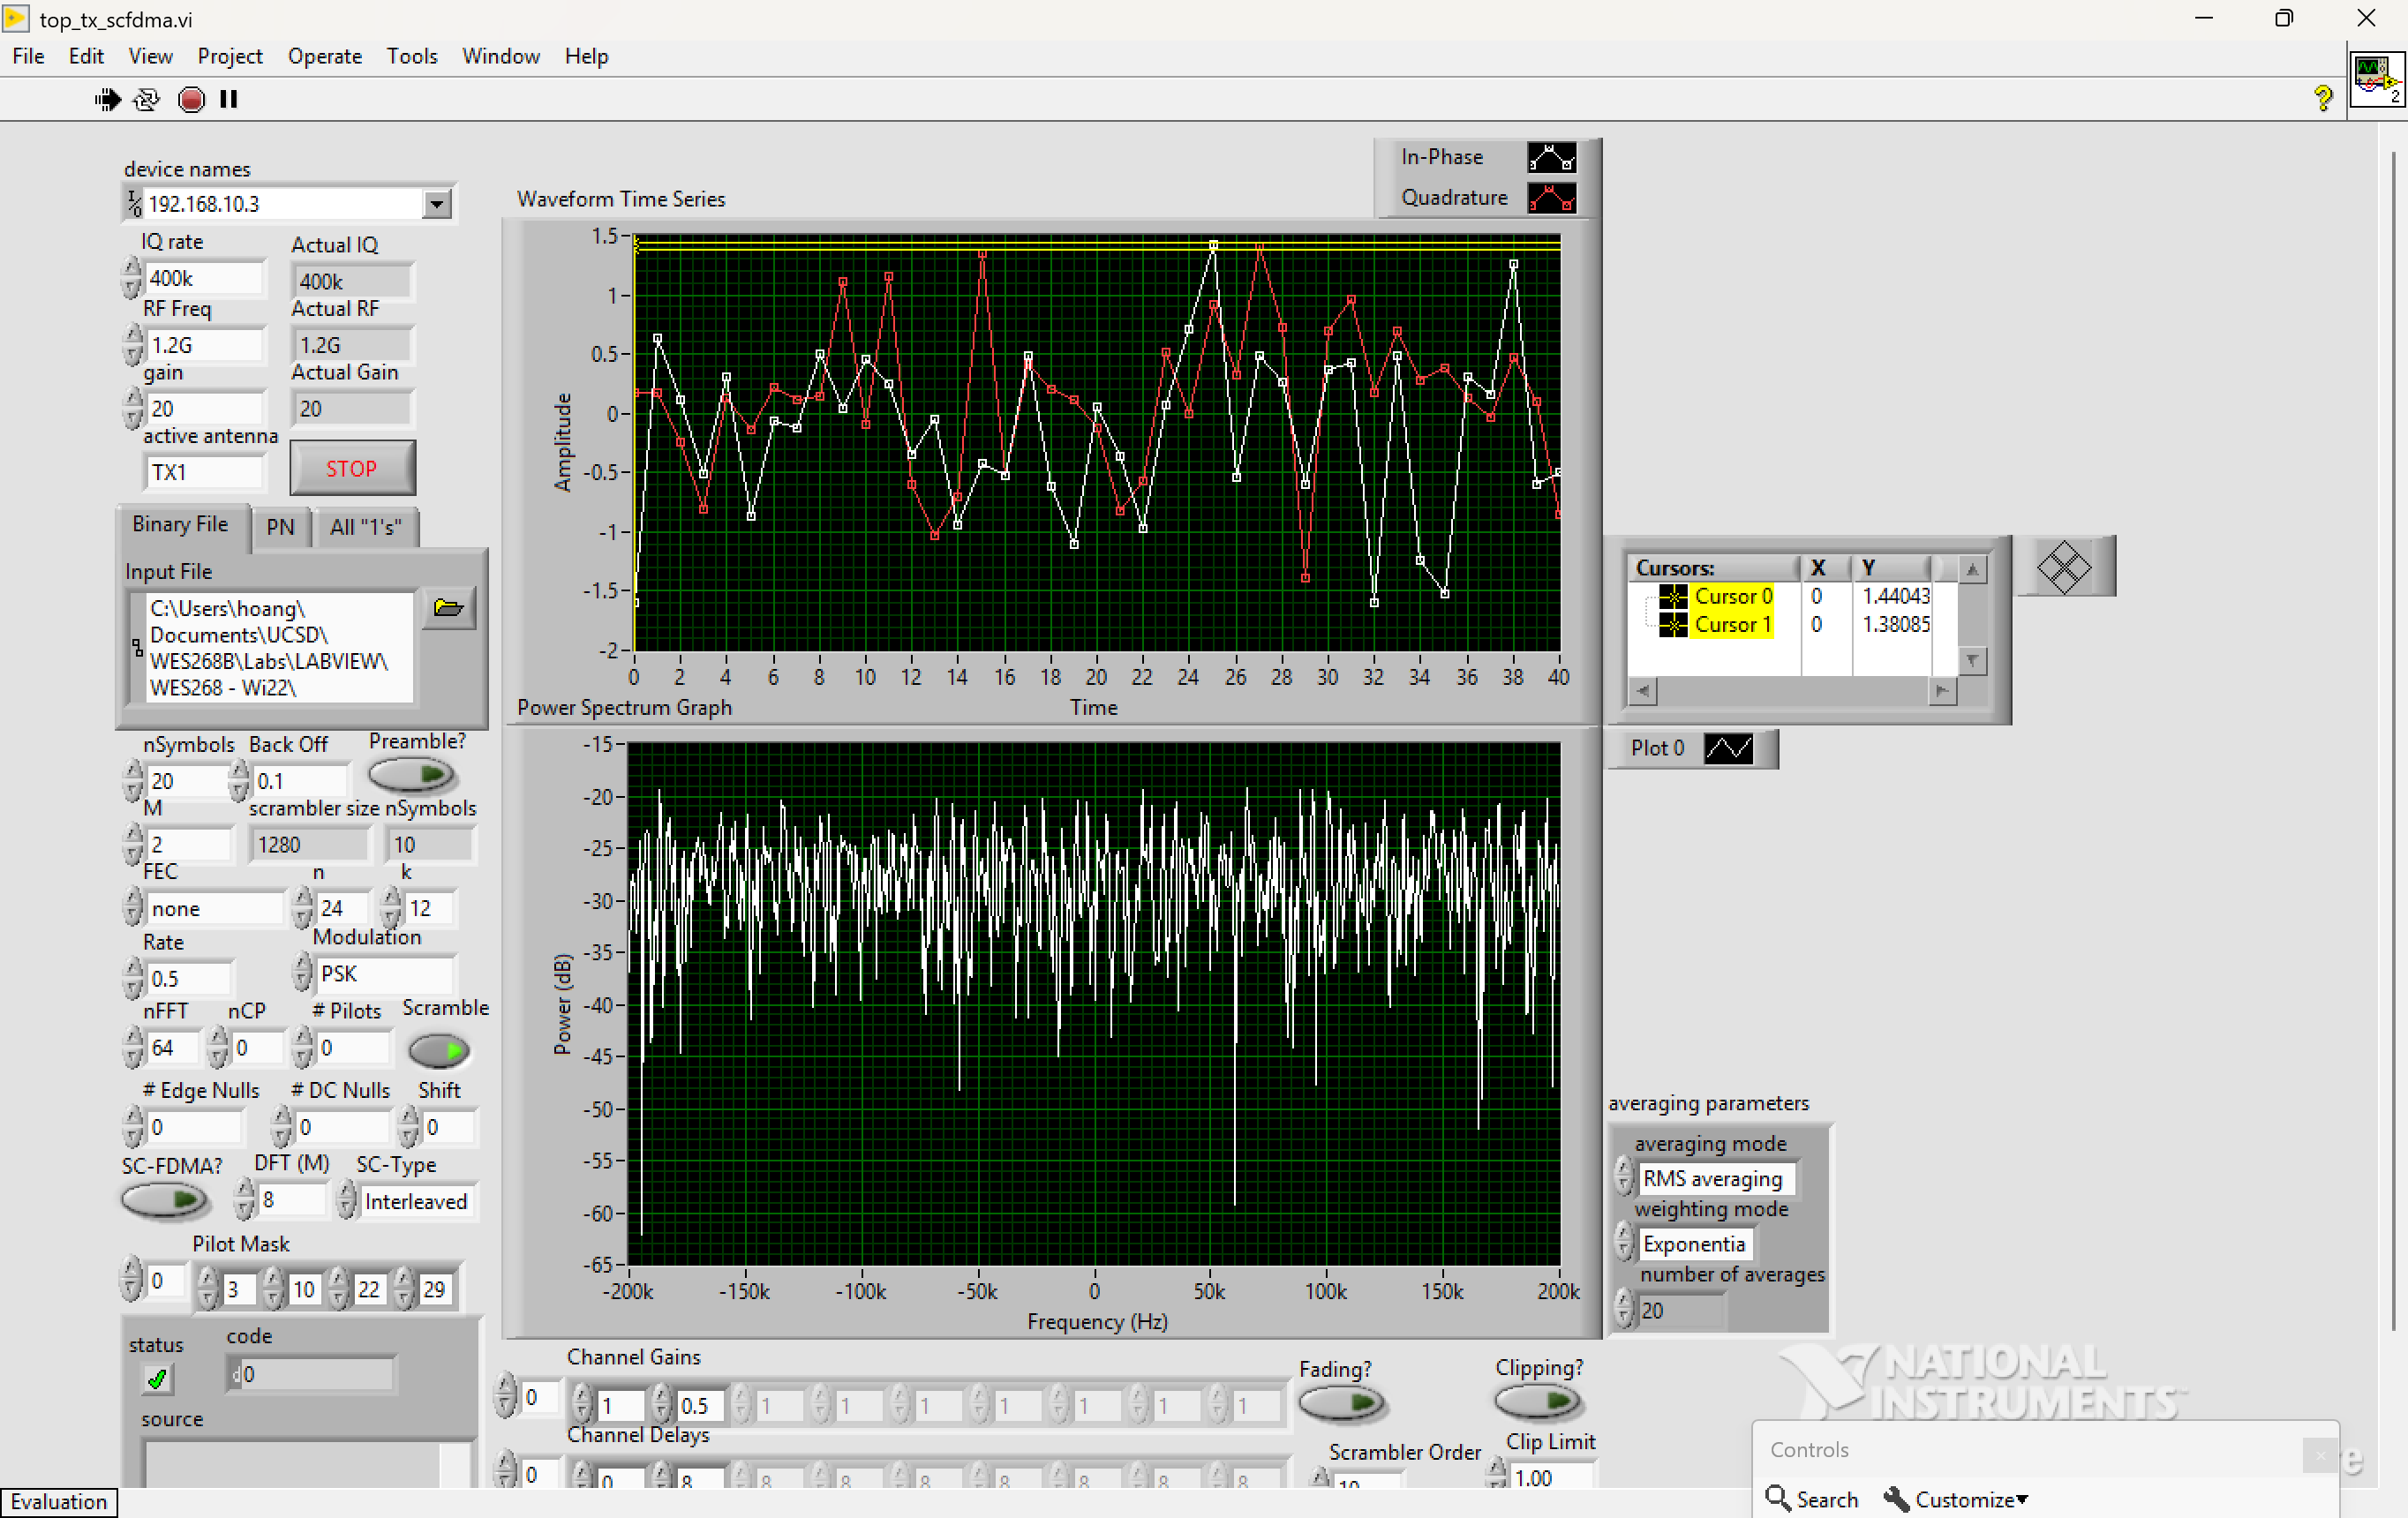
\includegraphics[width=0.7\textwidth]{lab_ss/WES268B_Lab7_Part2-1-2a_scramblerON_nFFT-64_PAPR-2p83dB.png}
    \caption{Lab 7 - Scrambler ON, Uncompressed File Input, FFT Size = 64, PAPR = 2.83dB}
    %\label{f26}
\end{figure}

\begin{figure}[H]
    \centering
    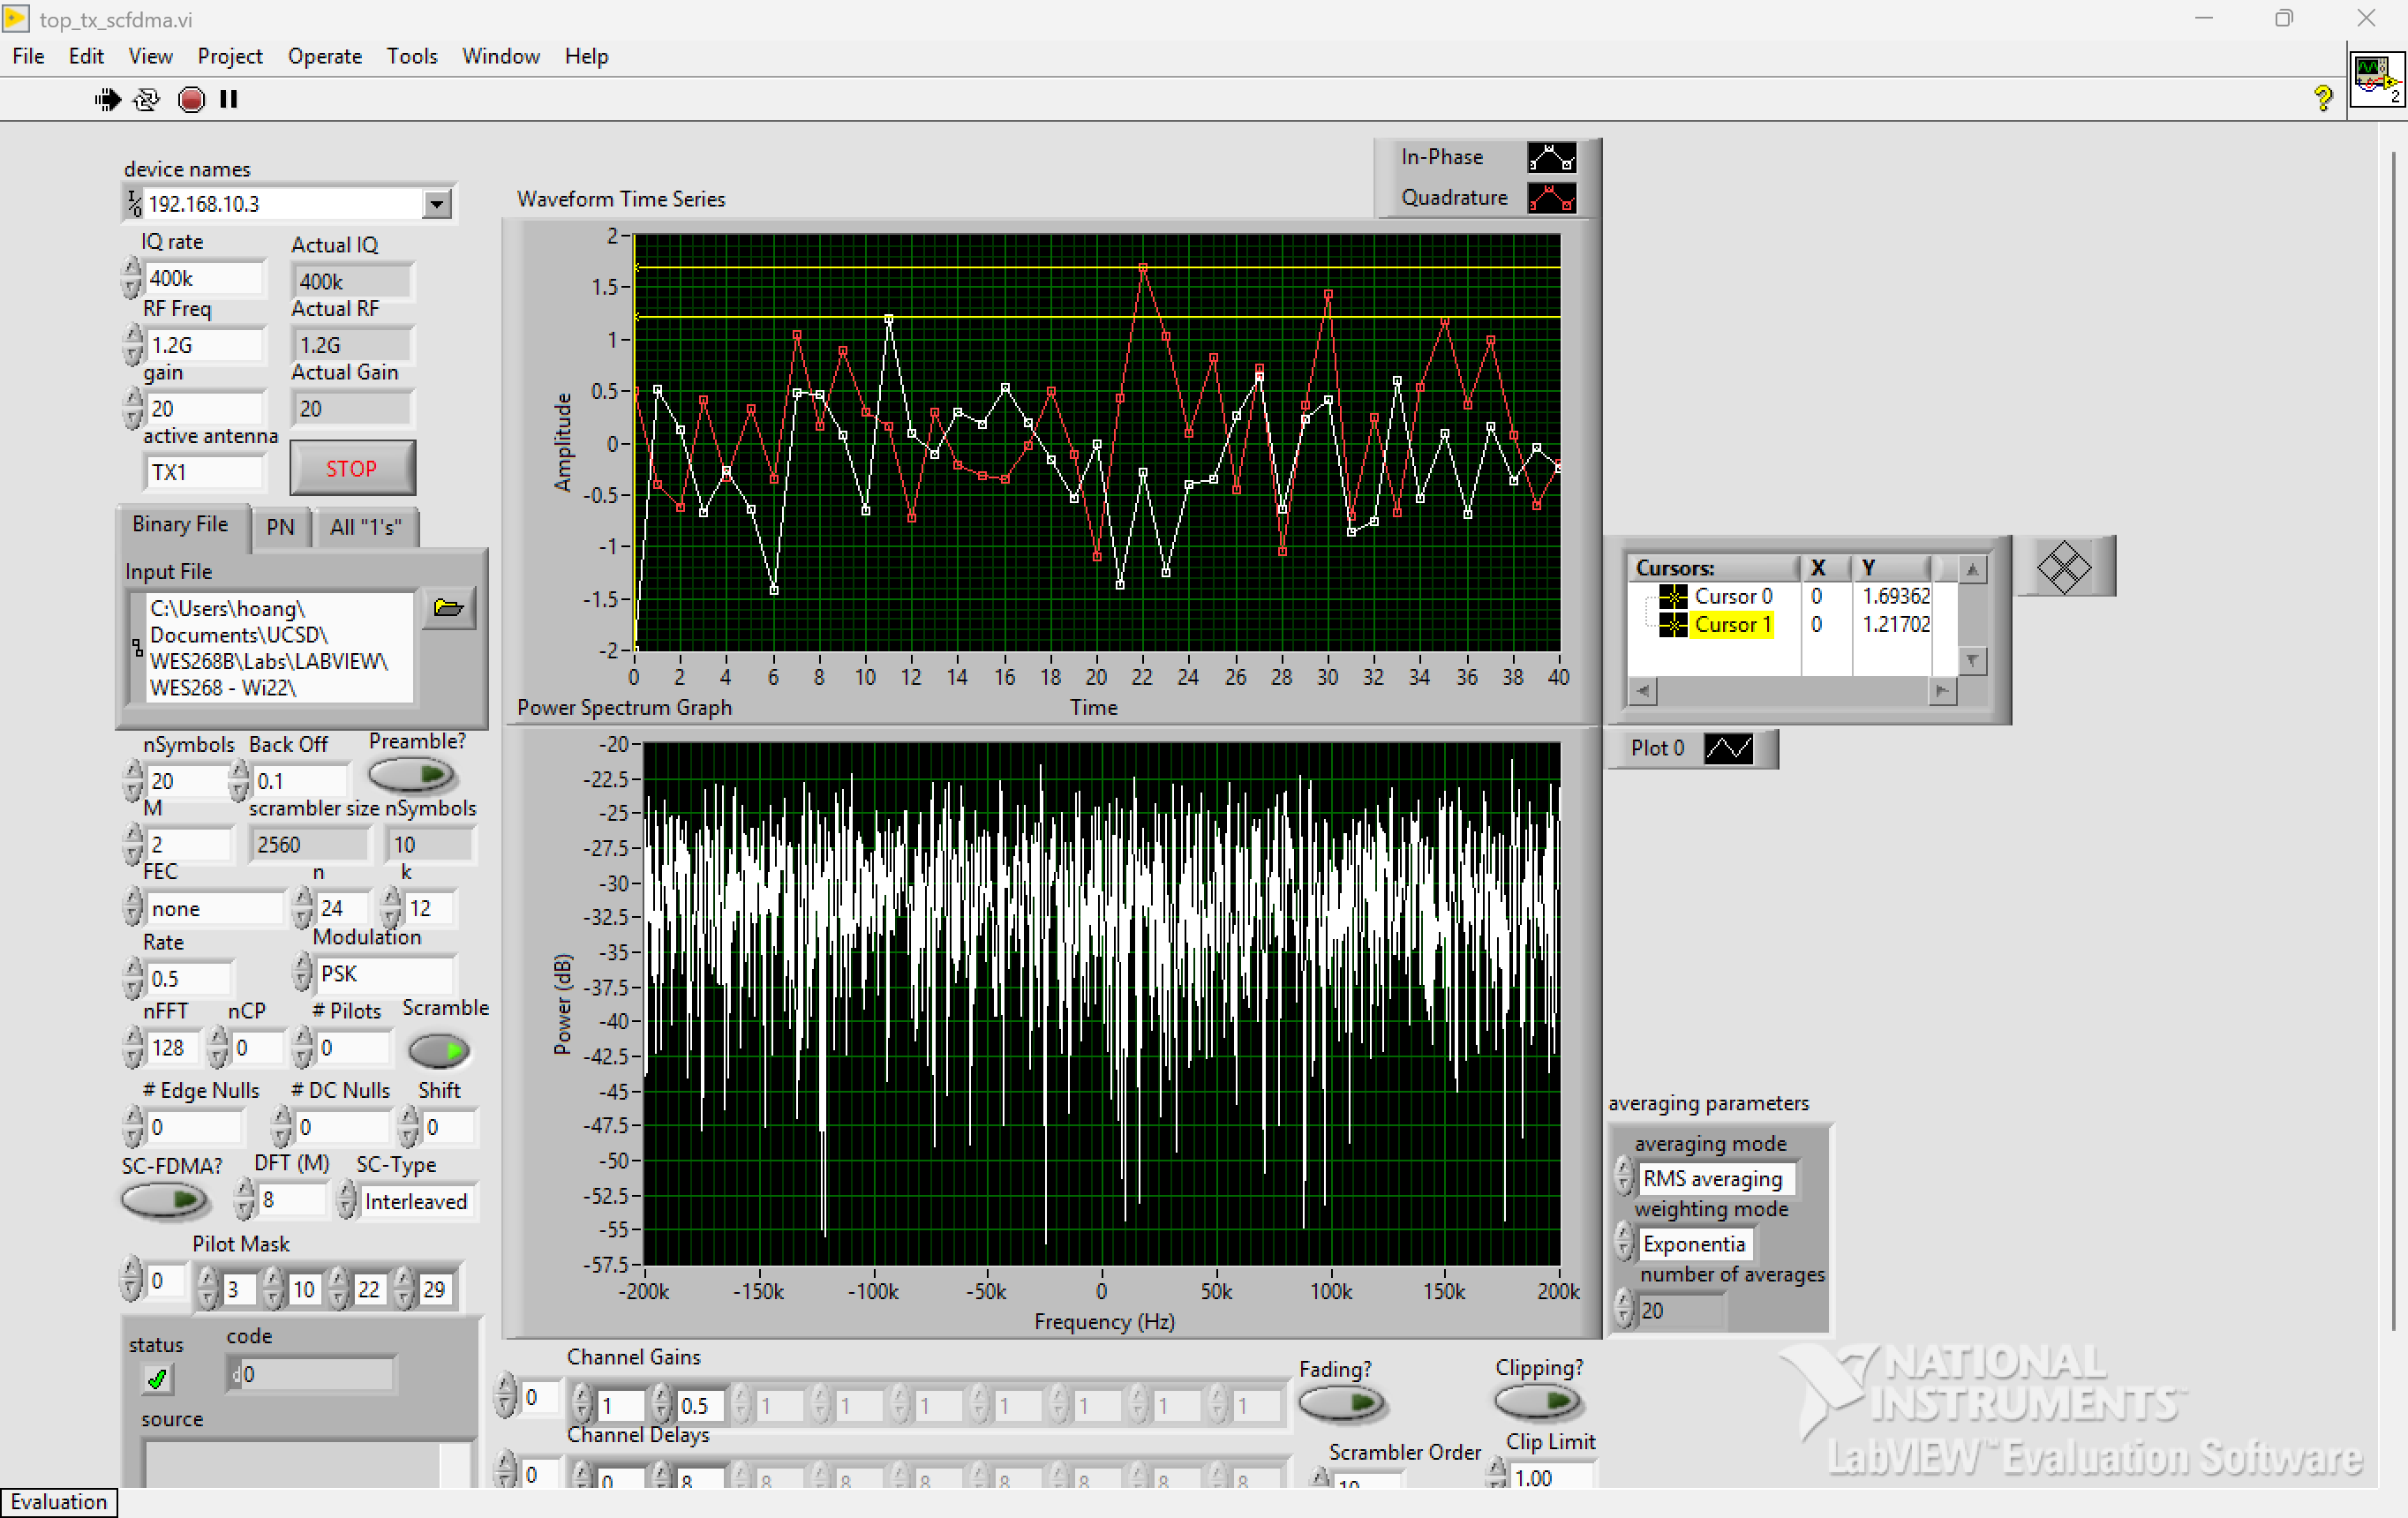
\includegraphics[width=0.7\textwidth]{lab_ss/WES268B_Lab7_Part2-1-2a_scramblerON_nFFT-128_PAPR-1p81dB.png}
    \caption{Lab 7 - Scrambler ON, Uncompressed File Input, FFT Size = 128, PAPR = 1.81dB}
    %\label{f27}
\end{figure}

\begin{figure}[H]
    \centering
    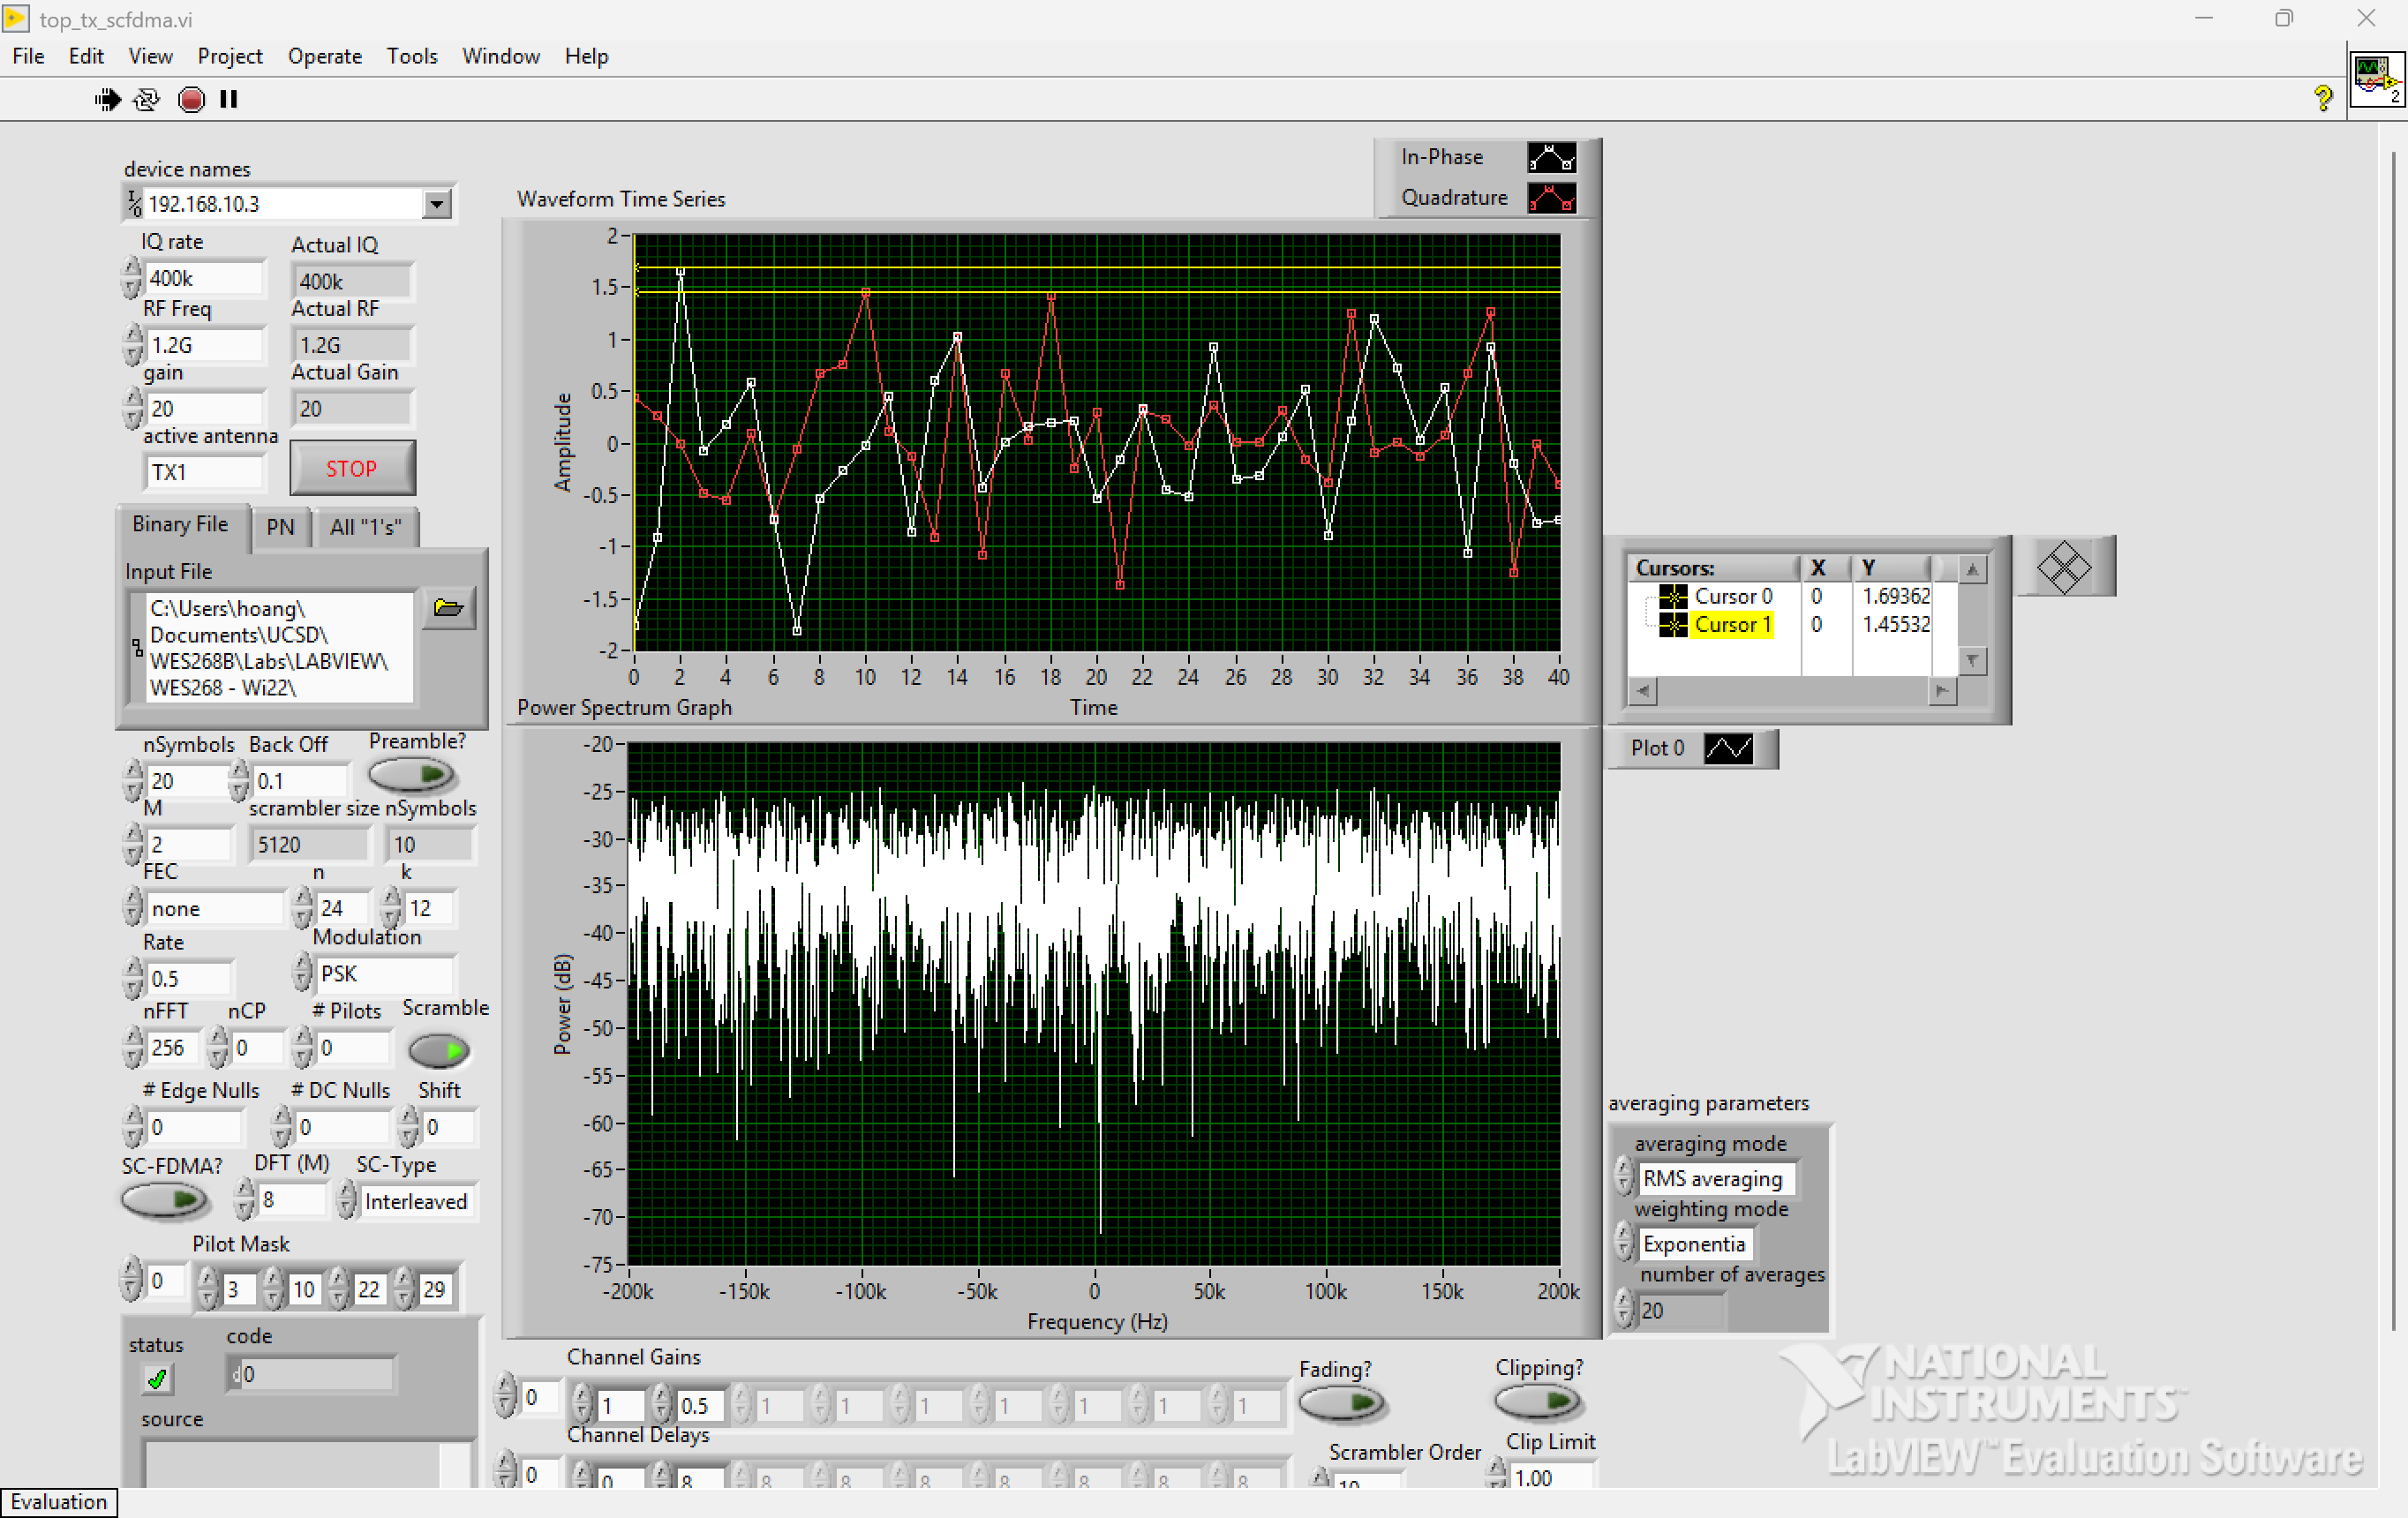
\includegraphics[width=0.7\textwidth]{lab_ss/WES268B_Lab7_Part2-1-2a_scramblerON_nFFT-256_PAPR-2p4dB.png}
    \caption{Lab 7 - Scrambler ON, Uncompressed File Input, FFT Size = 256, PAPR = 2.4dB}
    %\label{f28}
\end{figure}

% 2.1.3
\subsubsection{ }
\noindent\textbf{Question.}
{ 
    Is the scrambled PAPR always better than the unscrambled? Comment on your results. 
}
\noindent\textbf{Answer.} 
{
    In cases where the input data has repeated structures, then scrambled PAPR generally performs better than unscrambled 
    in terms of PAPR because it "breaks up" the repeated chunks and spreads power more evenly across the spectrum. If the input 
    data is already scrambled, then the scrambler step doesn't necessarily improve the PAPR.   
}


% 2.1.4
\subsubsection{}
\begin{figure}[H]
    \centering
    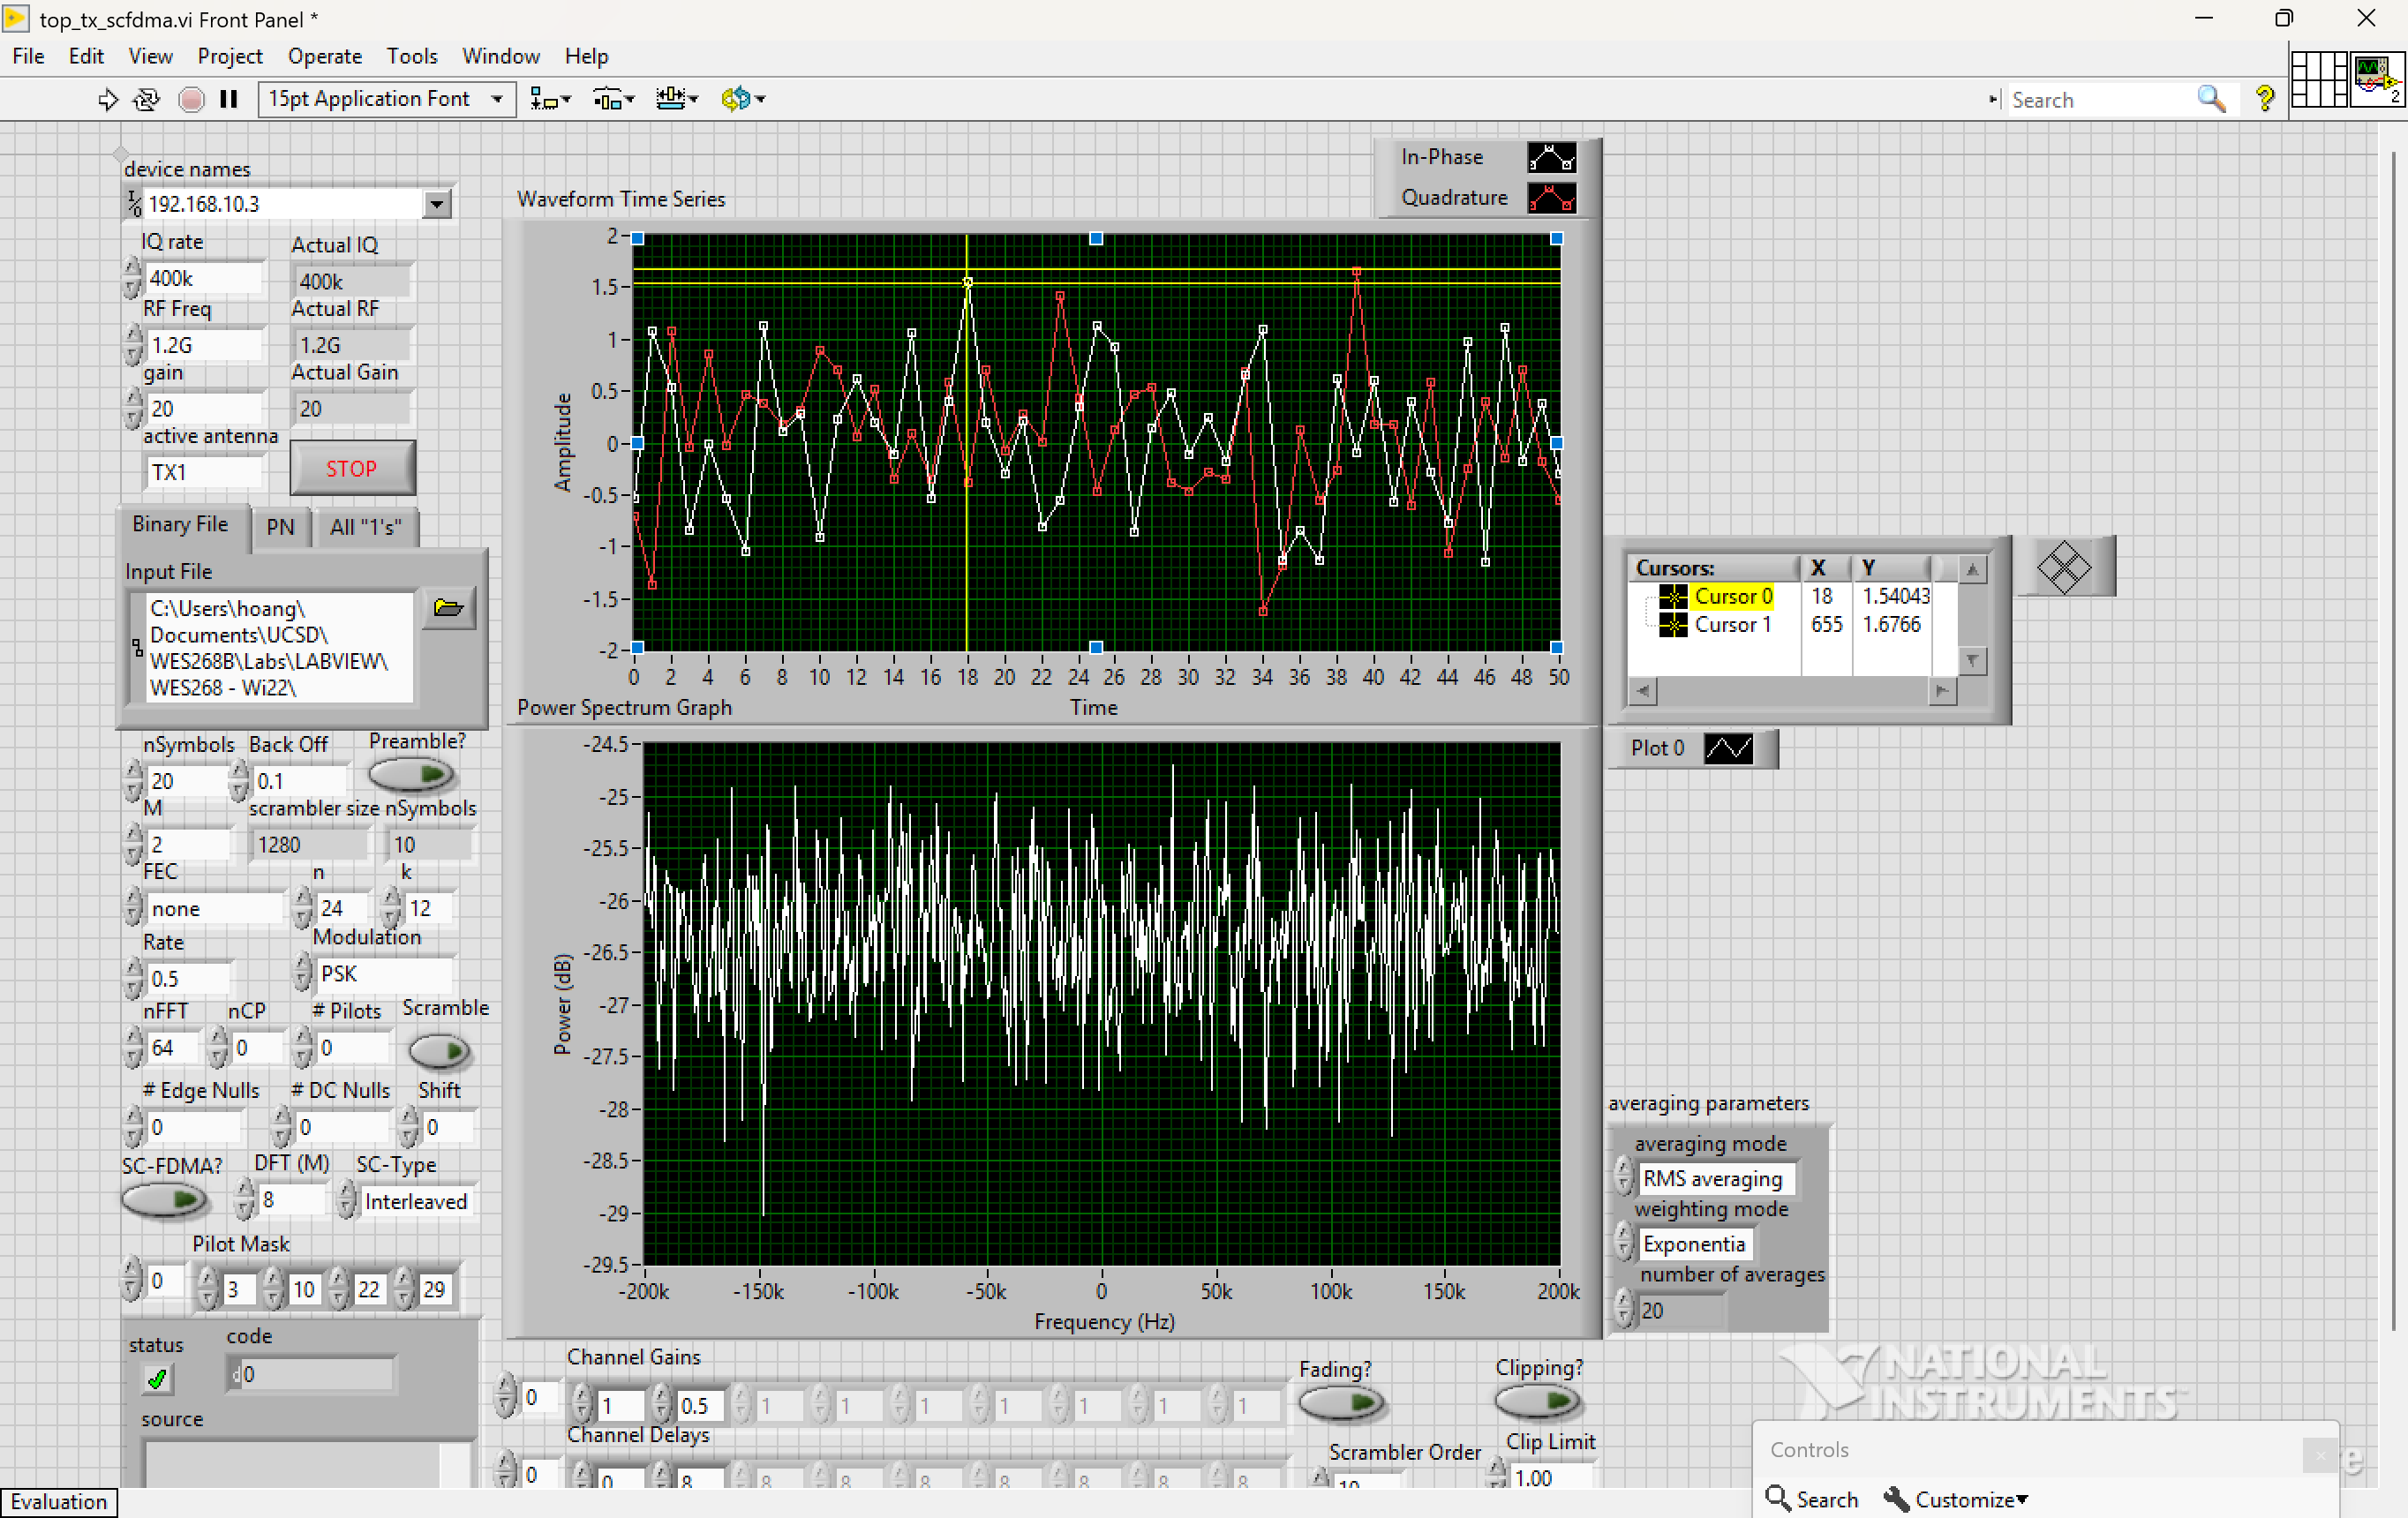
\includegraphics[width=0.7\textwidth]{lab_ss/WES268B_Lab7_Part2-1-4_scramblerOFF_compressedFile_nFFT-64_PAPR-2p8dB.png}
    \caption{Lab 7 - Scrambler OFF, Compressed File Input, FFT Size = 64, PAPR = 2.8dB}
    %\label{f29}
\end{figure}

\begin{figure}[H]
    \centering
    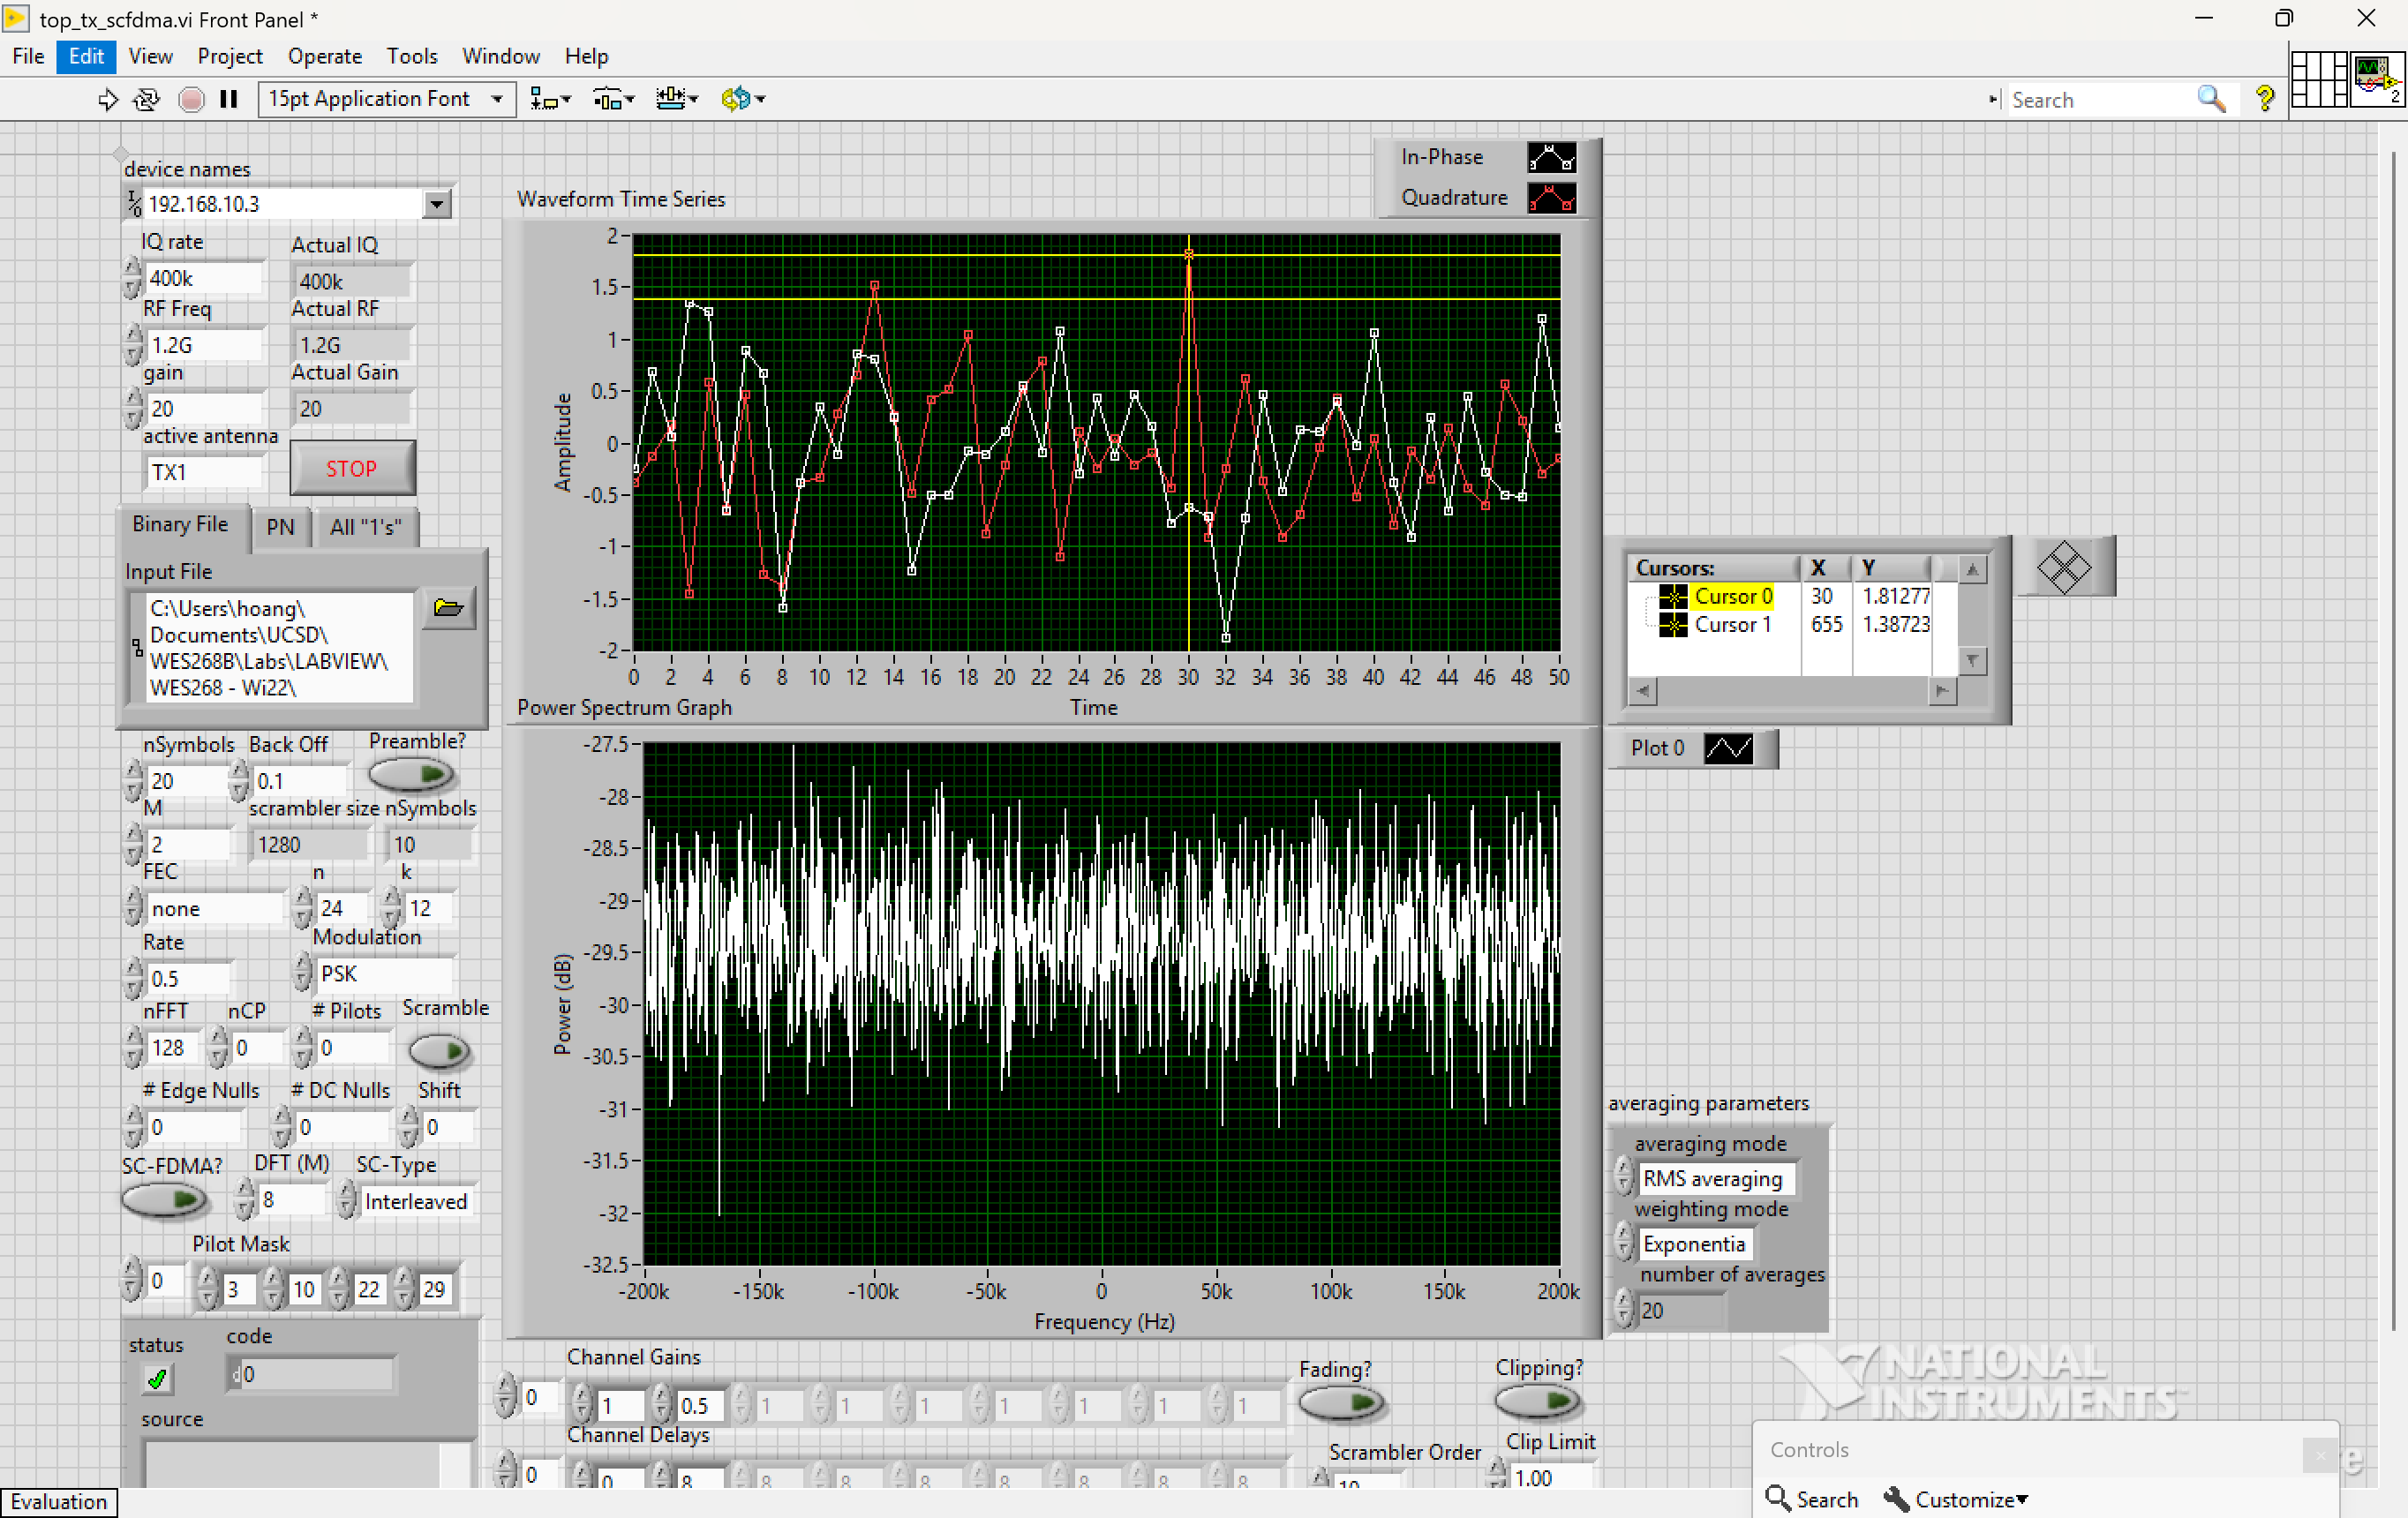
\includegraphics[width=0.7\textwidth]{lab_ss/WES268B_Lab7_Part2-1-4_scramblerOFF_compressedFile_nFFT-128_PAPR-2dB.png}
    \caption{Lab 7 - Scrambler OFF, Compressed File Input, FFT Size = 128, PAPR = 2dB}
    %\label{f30}
\end{figure}

\begin{figure}[H]
    \centering
    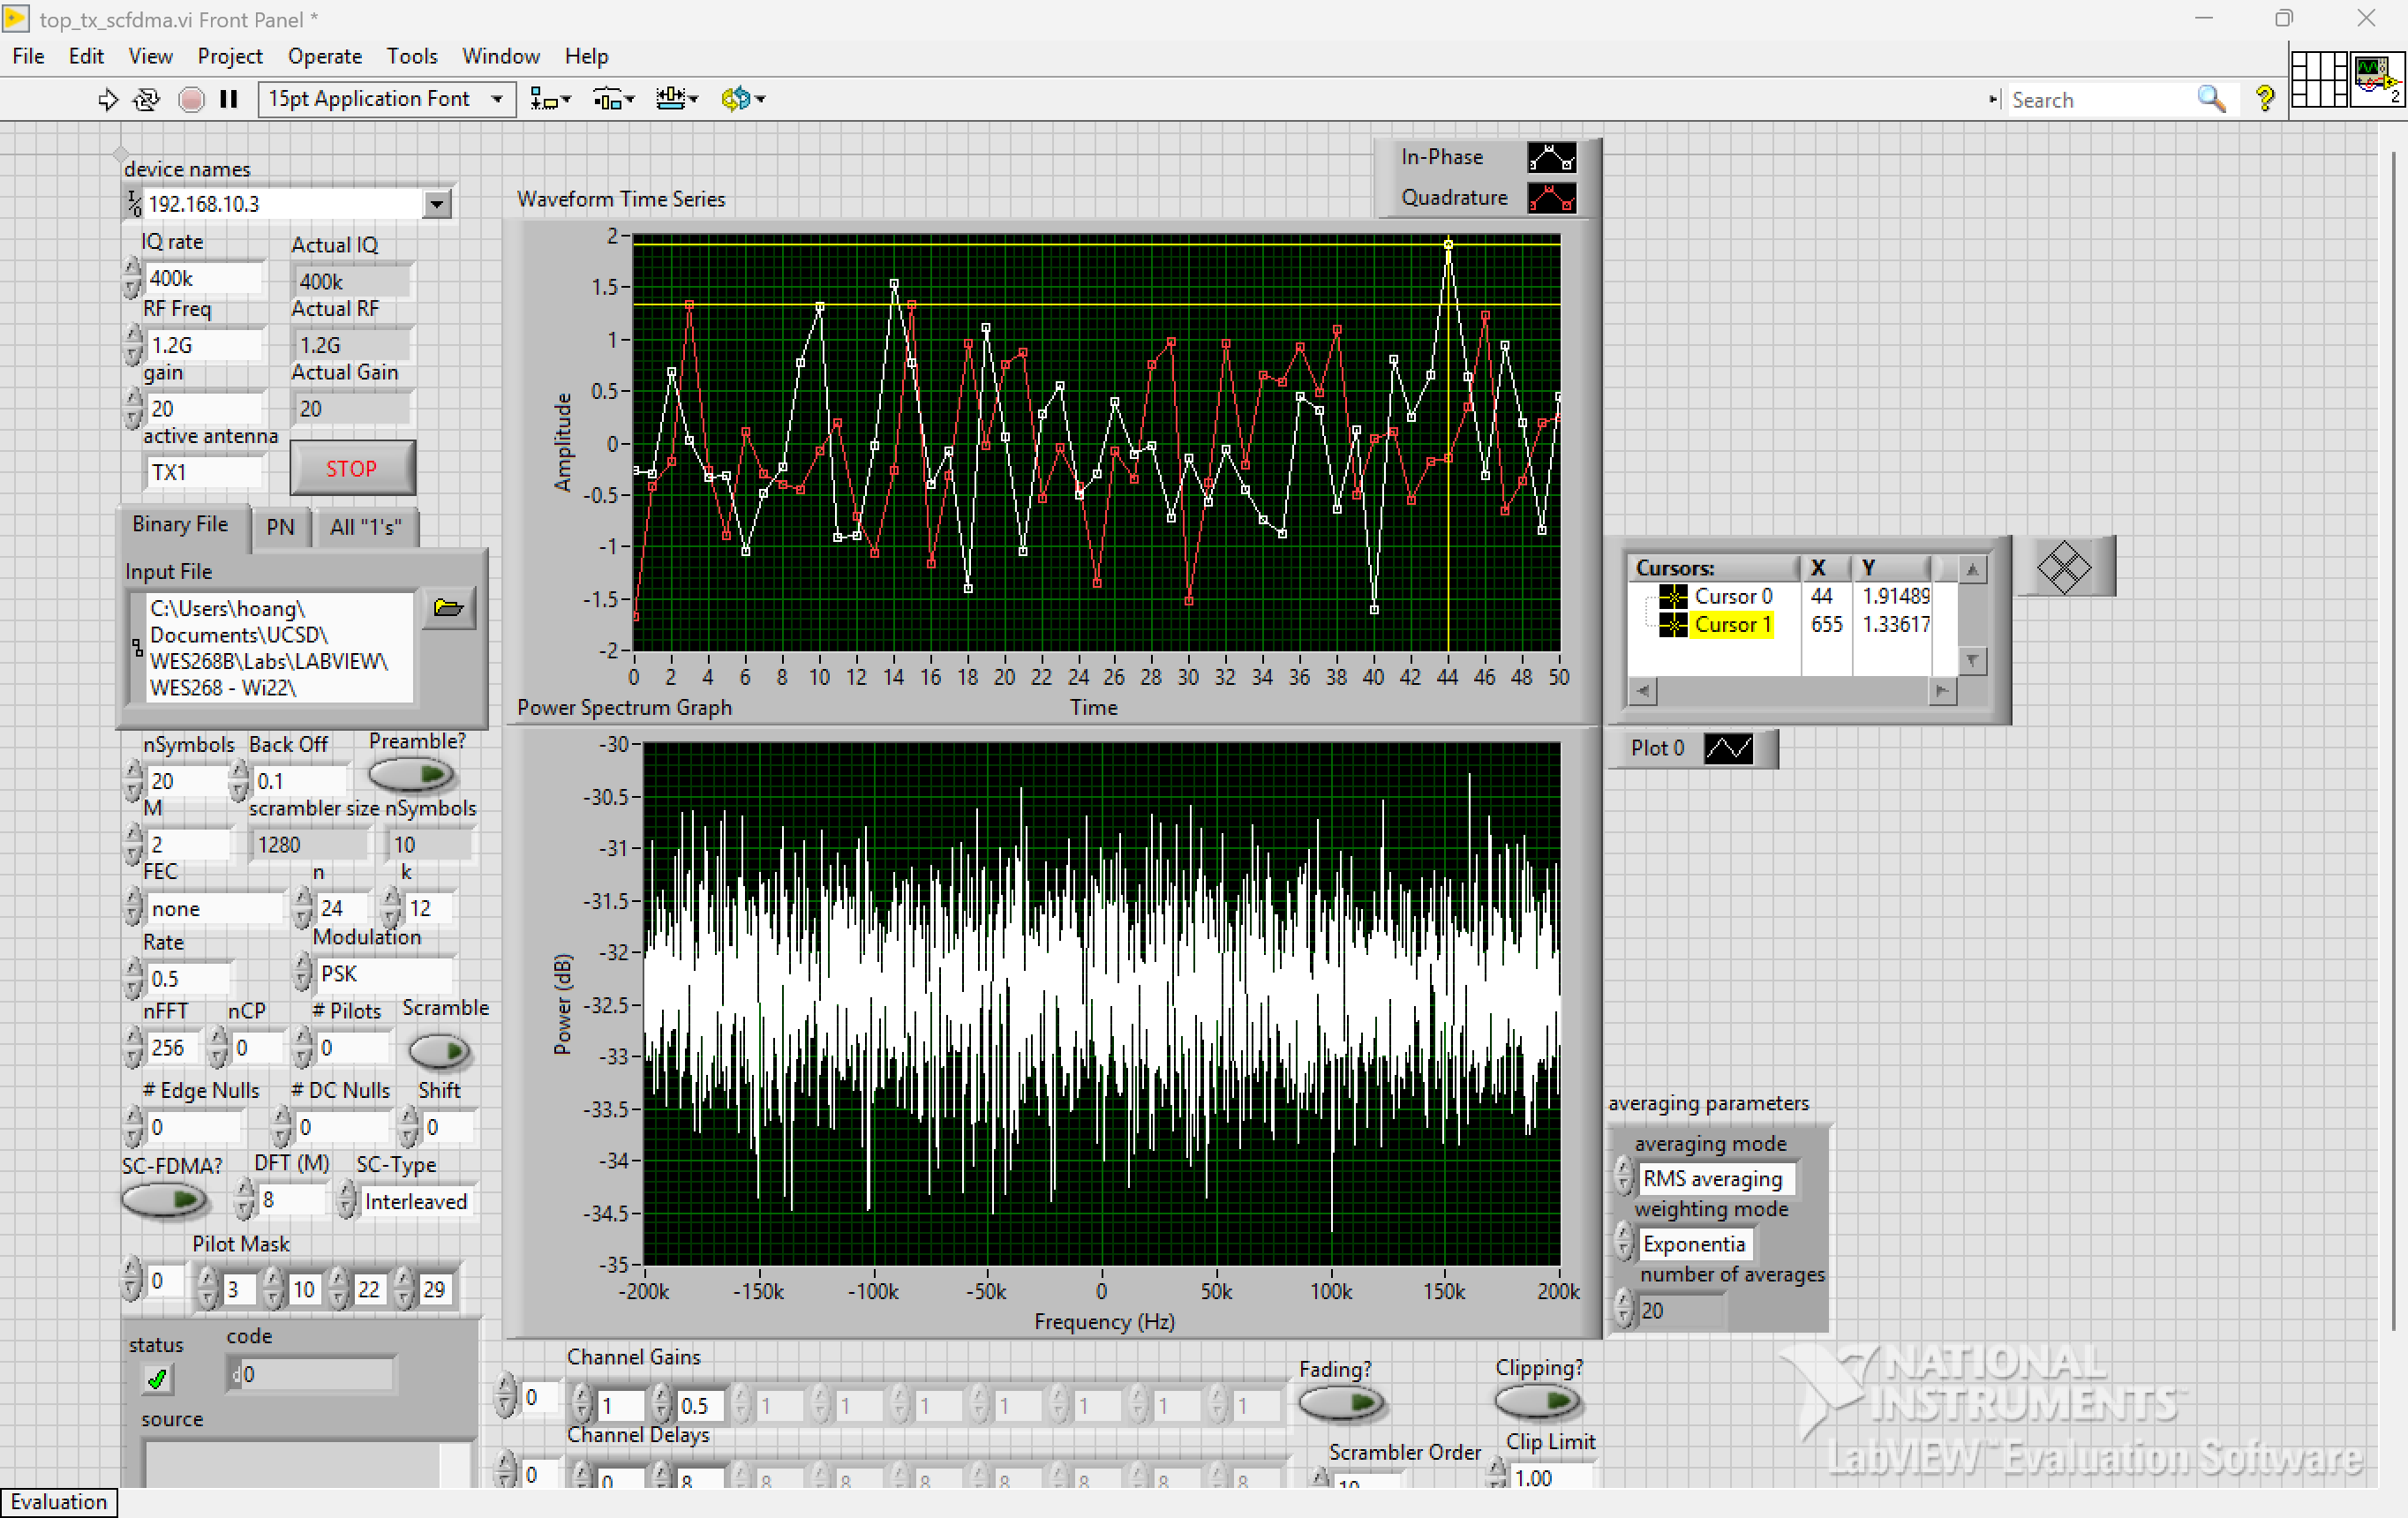
\includegraphics[width=0.7\textwidth]{lab_ss/WES268B_Lab7_Part2-1-4_scramblerOFF_compressedFile_nFFT-256_PAPR-1p7dB.png}
    \caption{Lab 7 - Scrambler OFF, Compressed File Input, FFT Size = 256, PAPR = 1.7dB}
    %\label{f31}
\end{figure}

\noindent\textbf{Question.}
{ 
    How does the PAPR compare to the \textit{UncompressedFile} on average?
}
\noindent\textbf{Answer.} 
{
    The PAPR of the compressed file with scrambler OFF is very similar to the Uncompressed File with the scrambler ON. This is because 
    compressed data looks more random than the uncompressed data, so a scrambler is redundant.
}

% 2.1.5
\subsubsection{ }

% 2.1.6
\subsubsection{ }

% 2.1.7
\subsubsection{}
\begin{figure}[H]
    \centering
    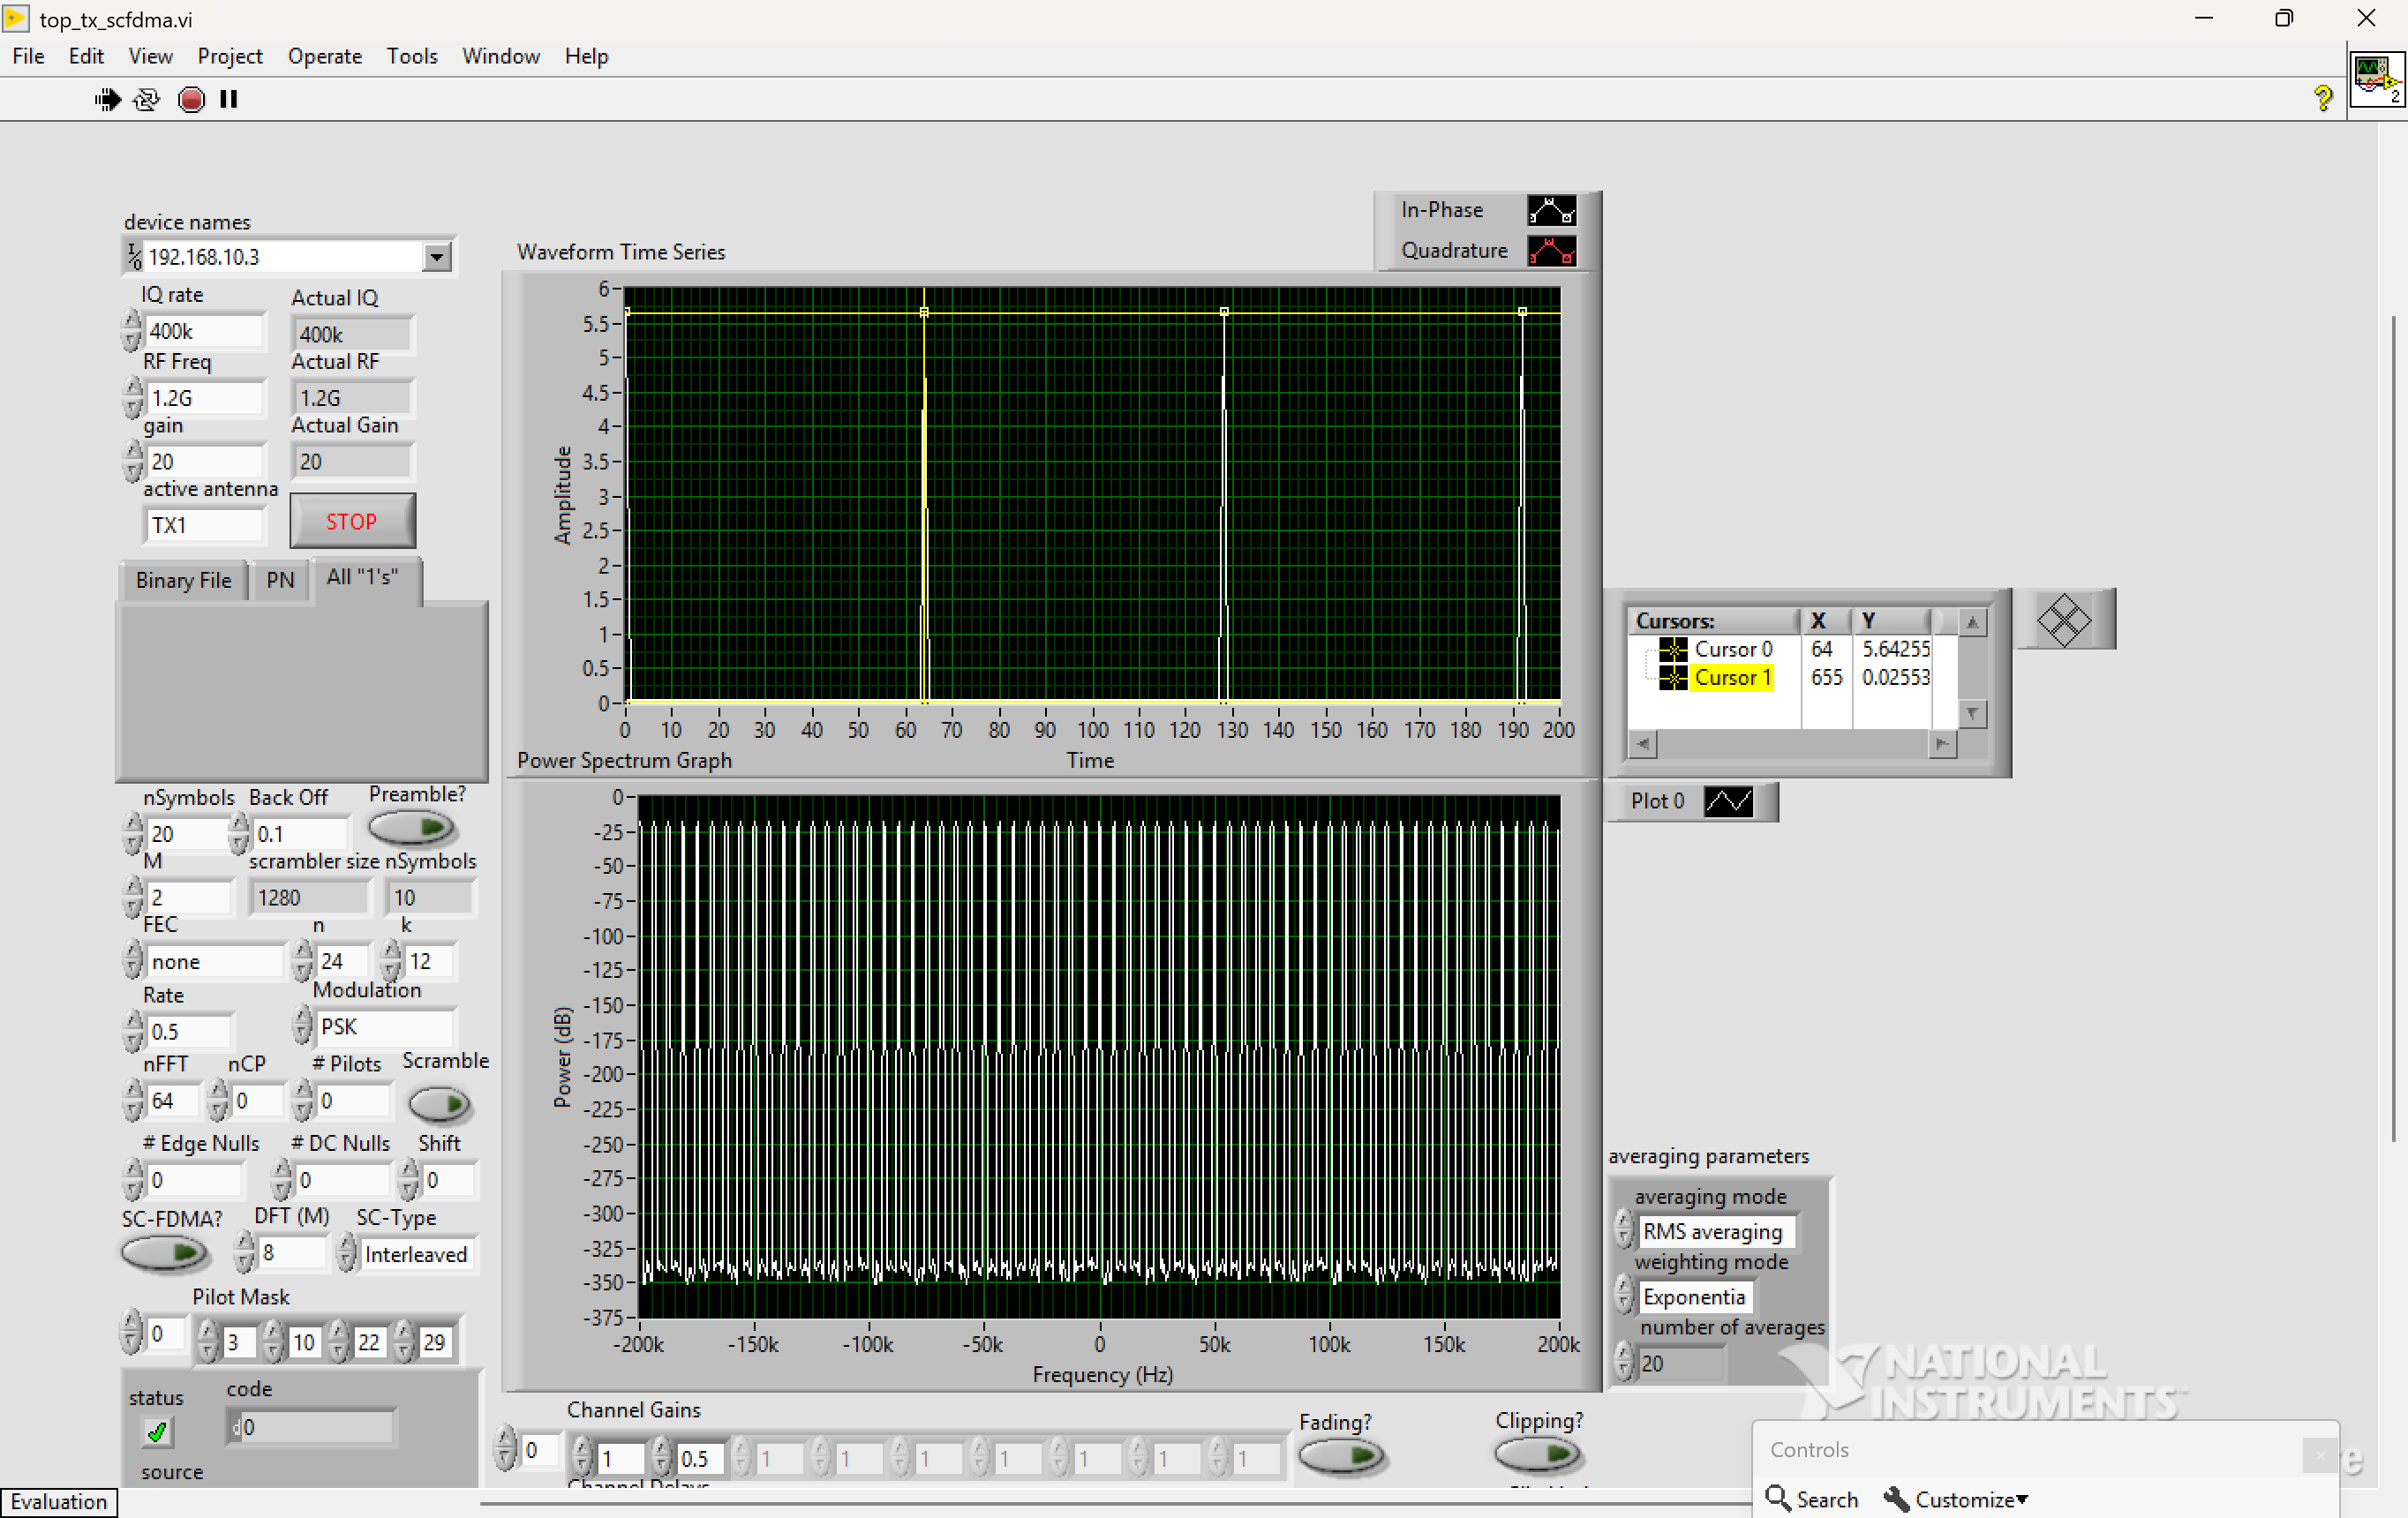
\includegraphics[width=0.7\textwidth]{lab_ss/WES268B_Lab7_Part2-1-7_scramblerOFF_all1s_nFFT-64_PAPR-18dB_idk.png}
    \caption{Lab 7 - Scrambler OFF, All 1's, FFT size = 64, PAPR = 18dB}
    %\label{f32}
\end{figure}

\begin{figure}[H]
    \centering
    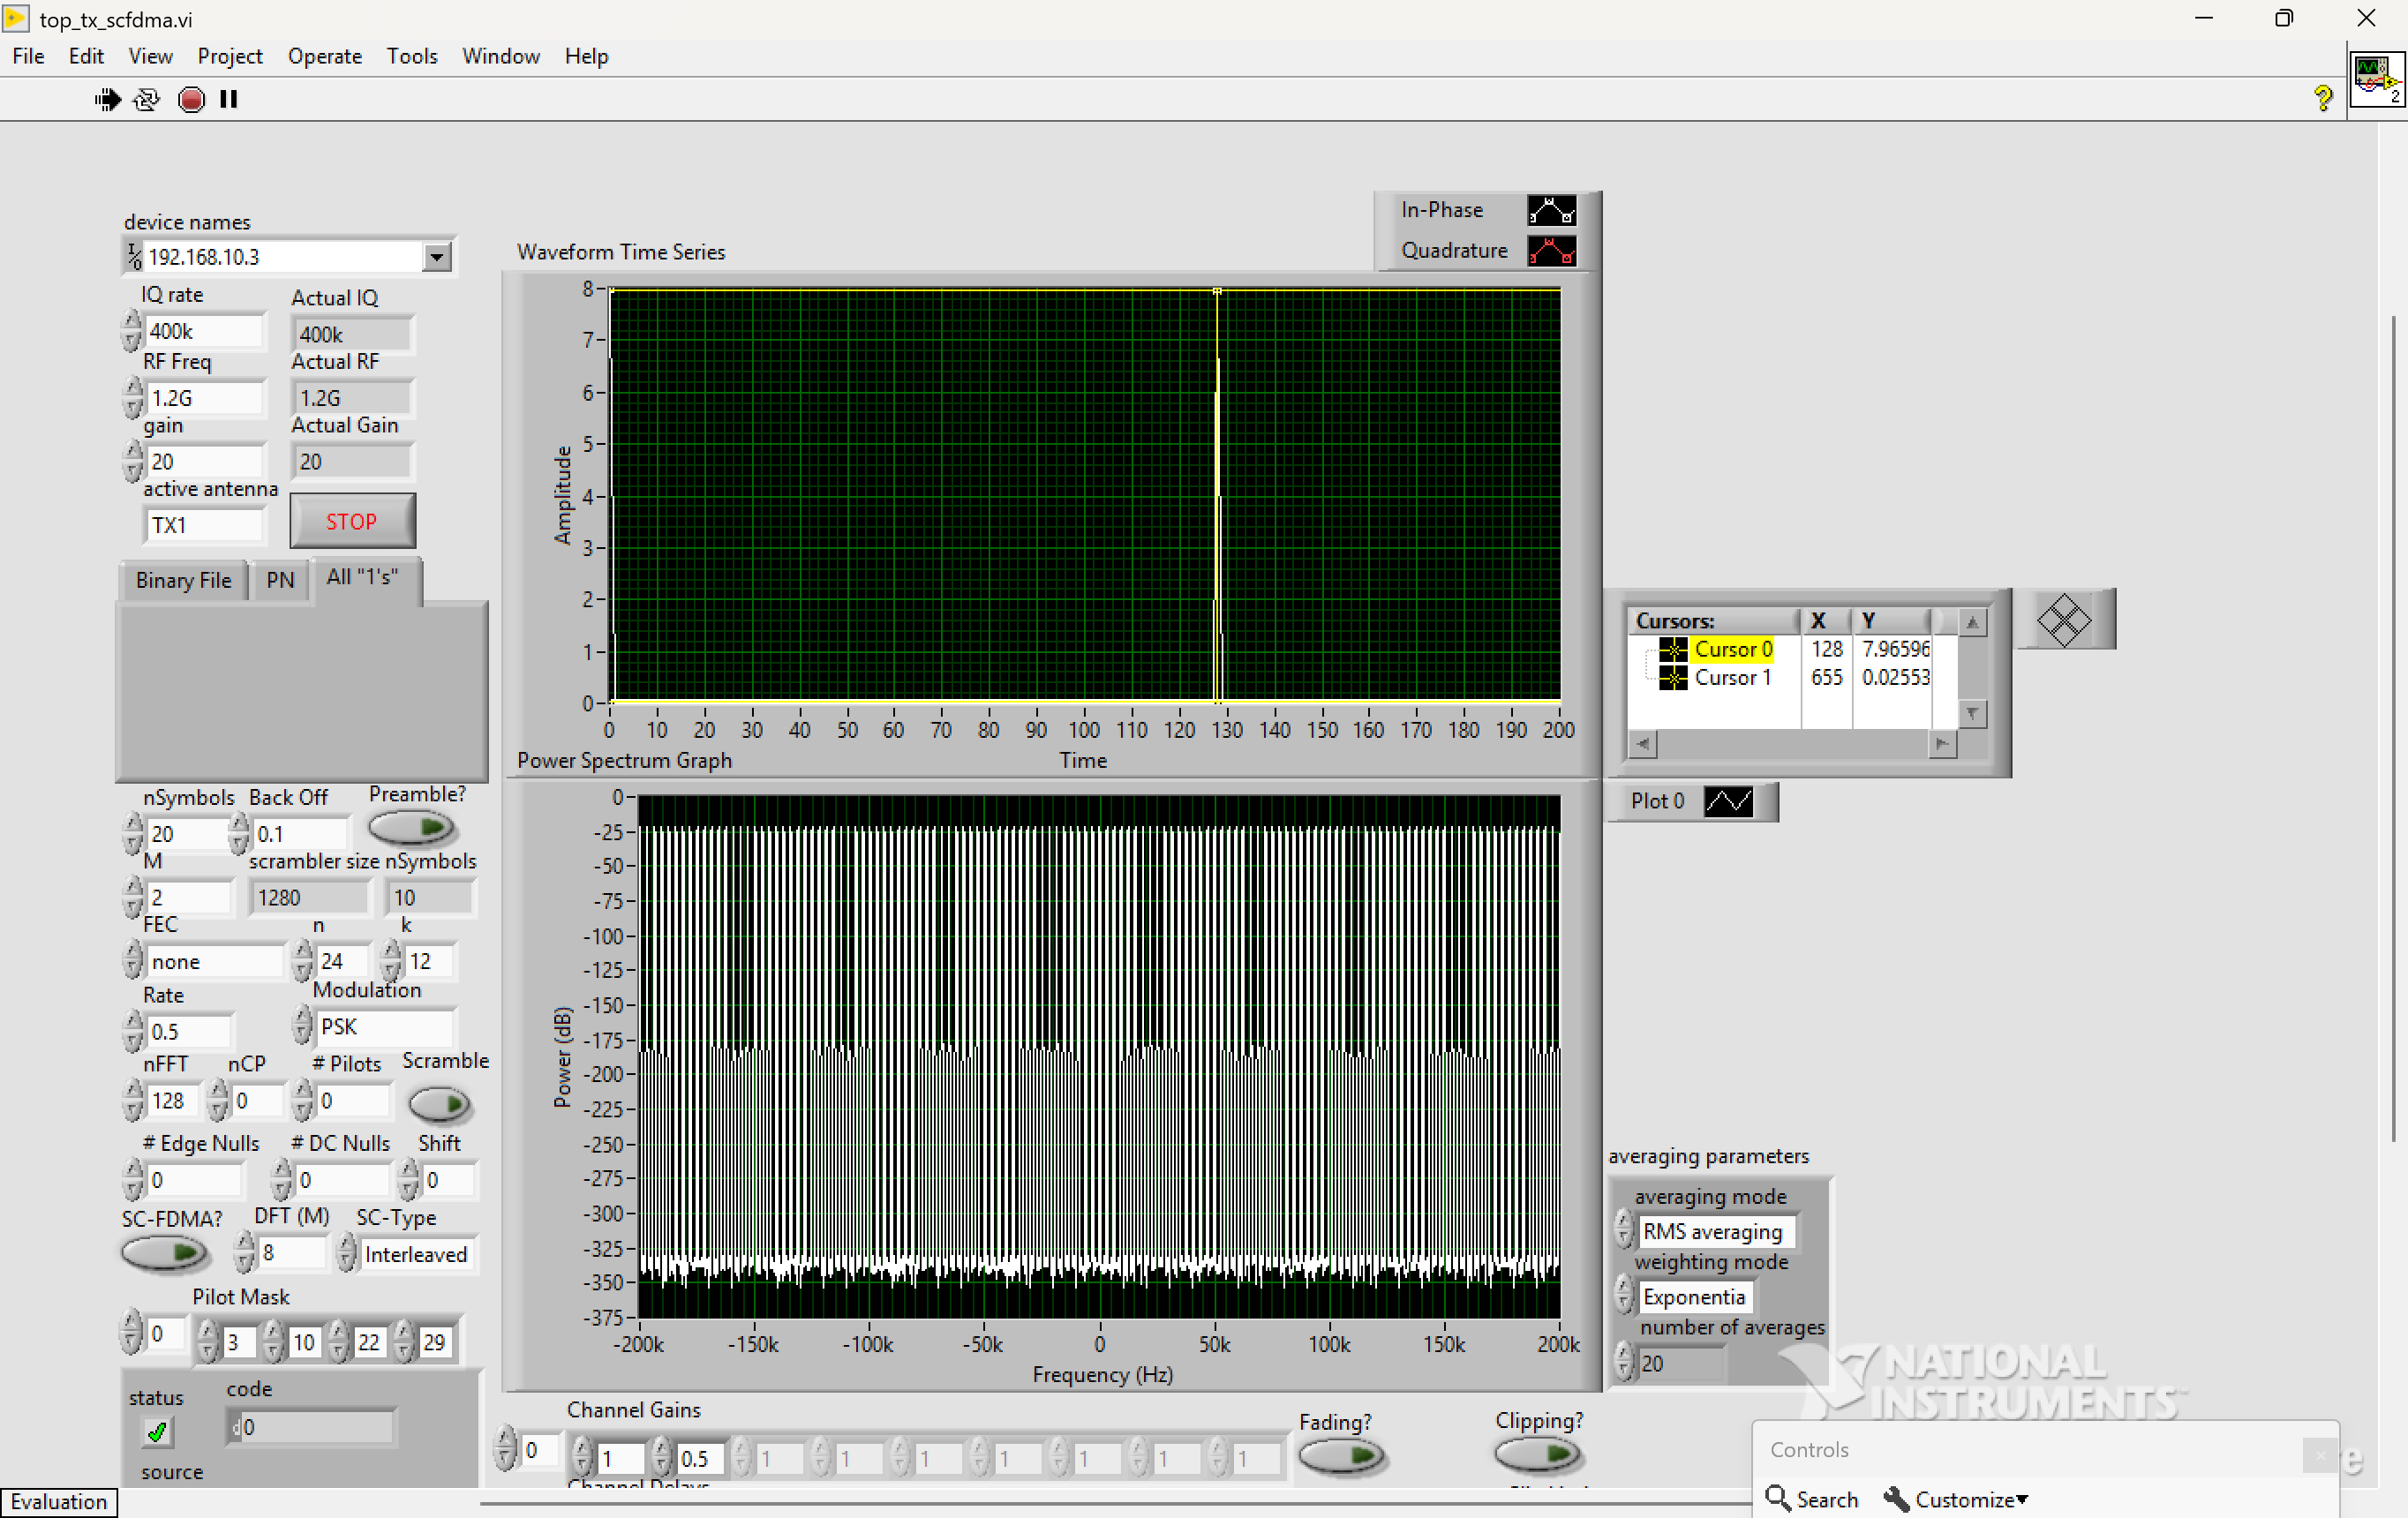
\includegraphics[width=0.7\textwidth]{lab_ss/WES268B_Lab7_Part2-1-7_scramblerOFF_all1s_nFFT-128_PAPR-21dB_idk.png}
    \caption{Lab 7 - Scrambler OFF, All 1's, FFT size = 128, PAPR = 21dB}
    %\label{f33}
\end{figure}

\begin{figure}[H]
    \centering
    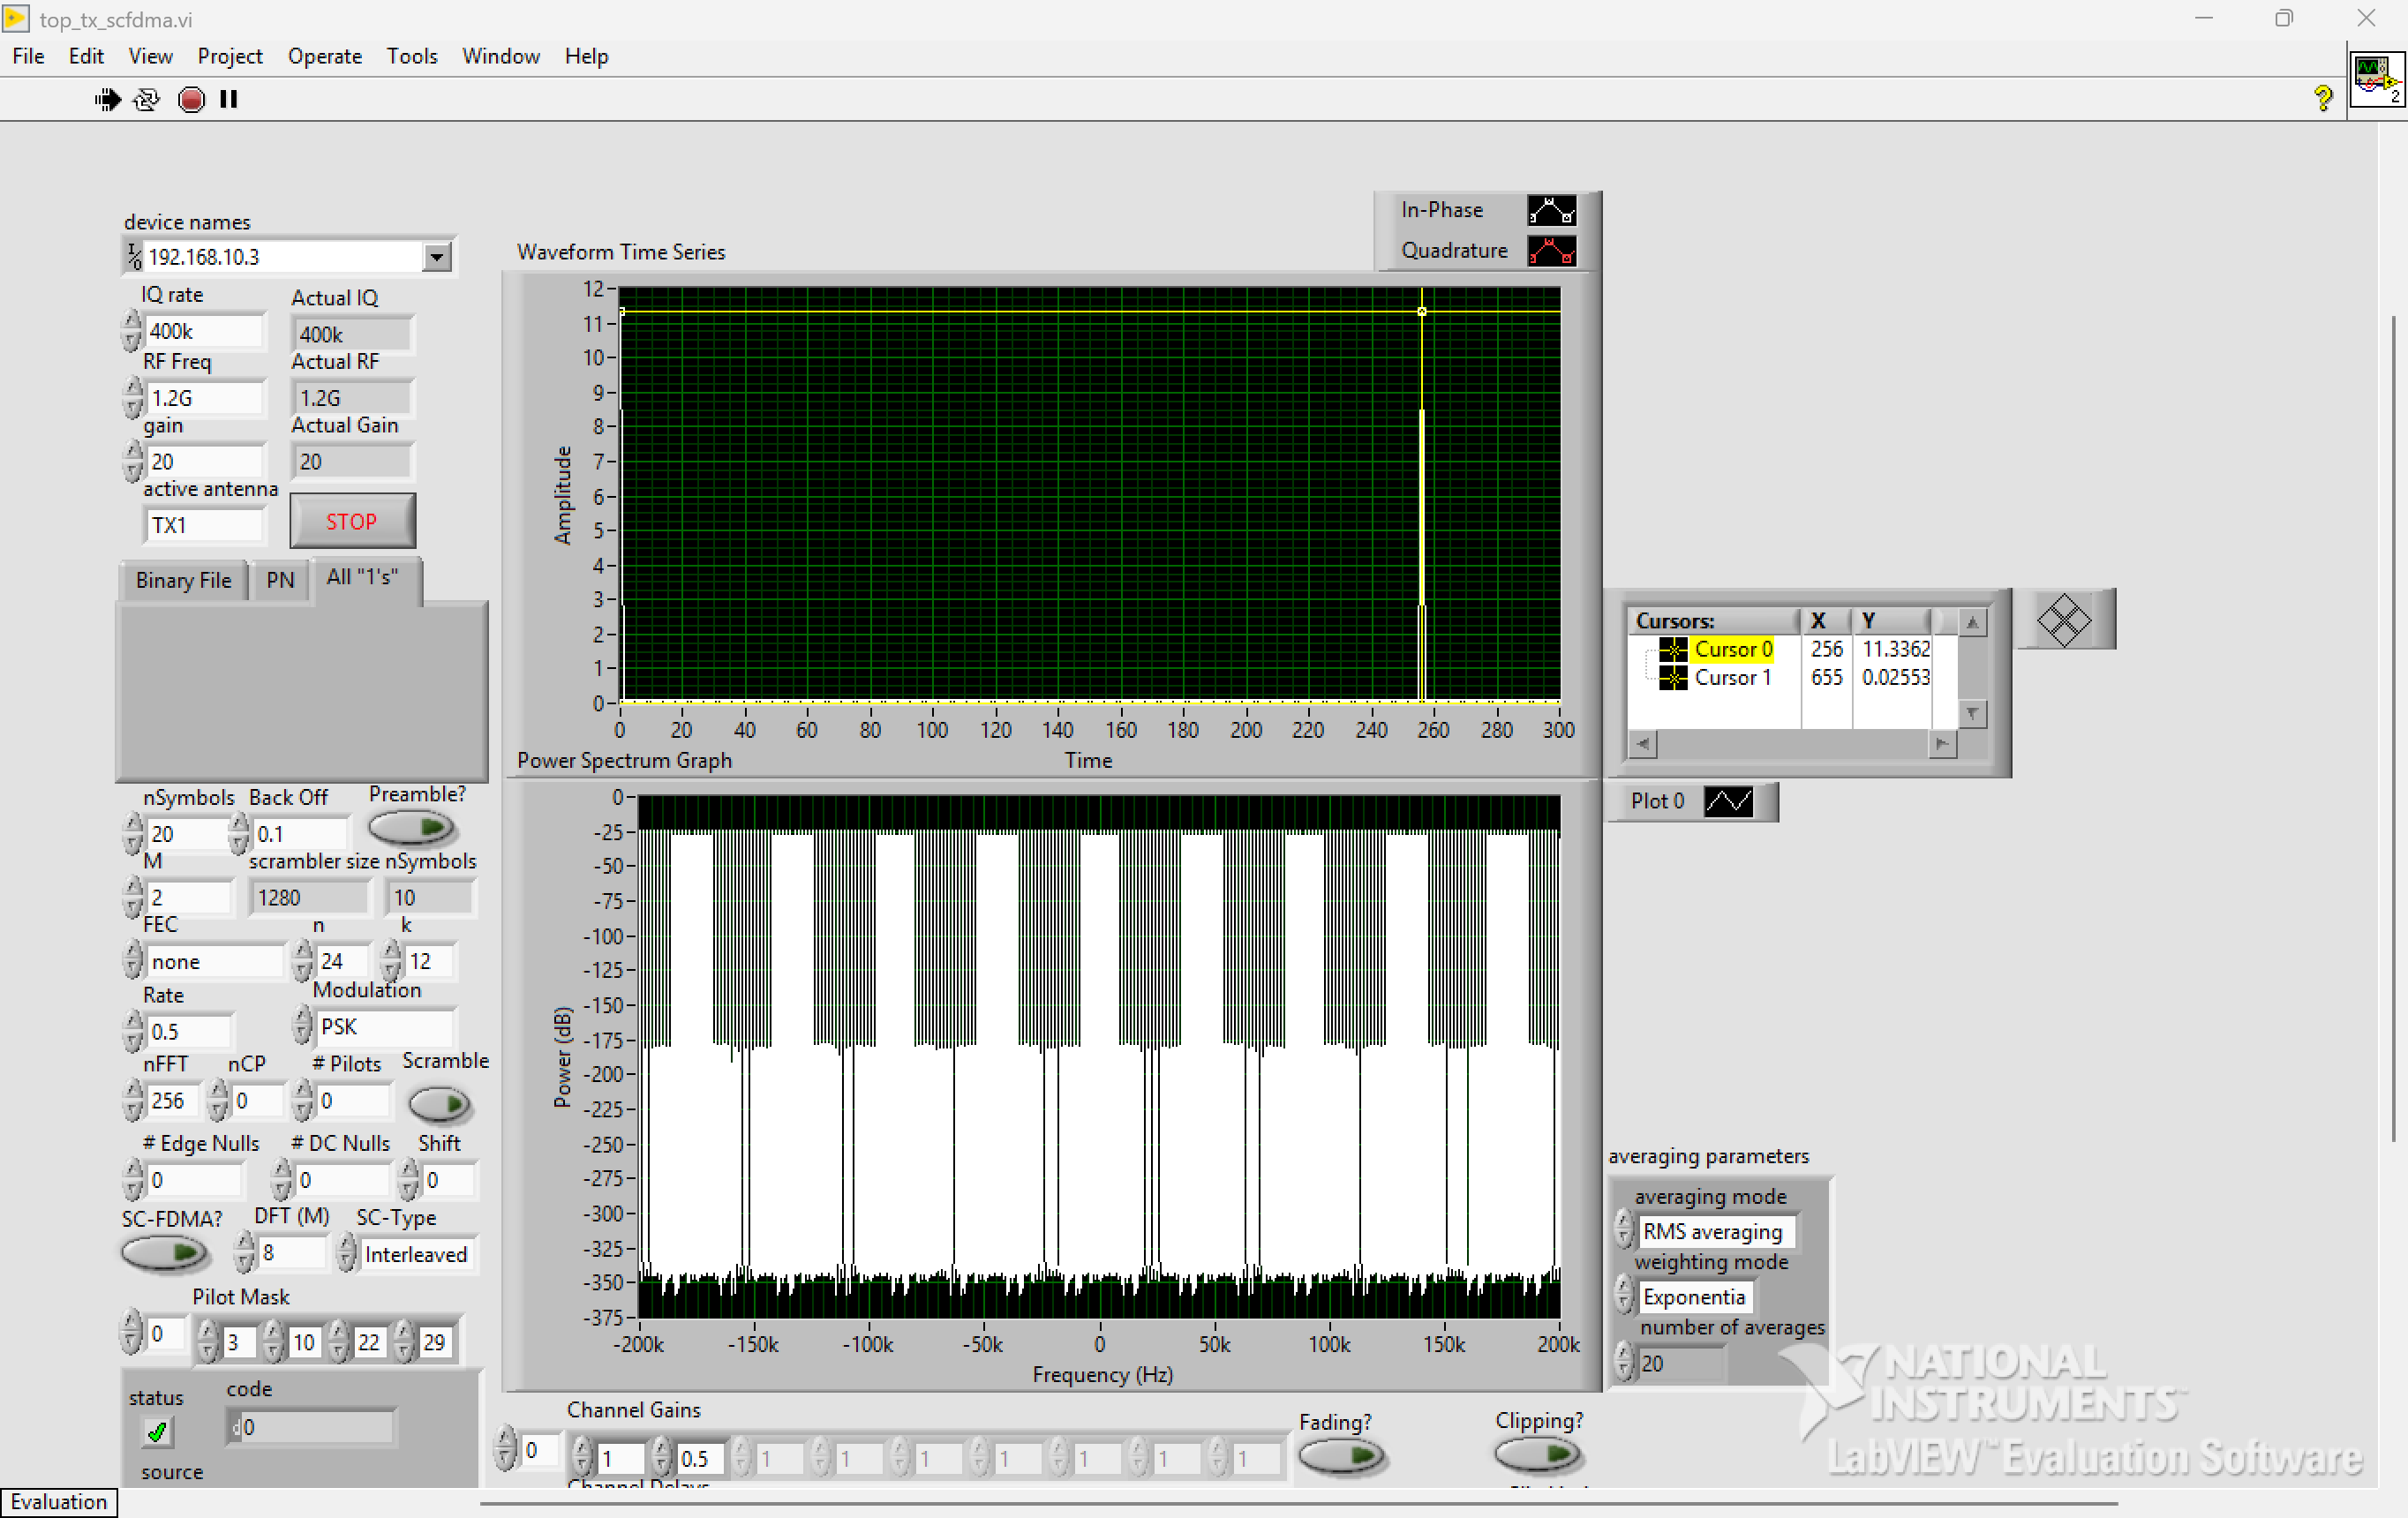
\includegraphics[width=0.7\textwidth]{lab_ss/WES268B_Lab7_Part2-1-7_scramblerOFF_all1s_nFFT-256_PAPR-24dB_idk.png}
    \caption{Lab 7 - Scrambler OFF, All 1's, FFT size = 256, PAPR = 24dB}
    %\label{f34}
\end{figure}
\noindent\textbf{Question.}
{ 
    Repeat step 2b) and comment on your results.
}
\noindent\textbf{Answer.} 
{
    Since the input stream is all 1s, the PAPR is very bad without the scrambler ON as seen in the figures above. Again, this is because 
    the data is highly structured and does not spread power evenly across the spectrum.
}

% 2.1.8
\subsubsection{}
\begin{figure}[H]
    \centering
    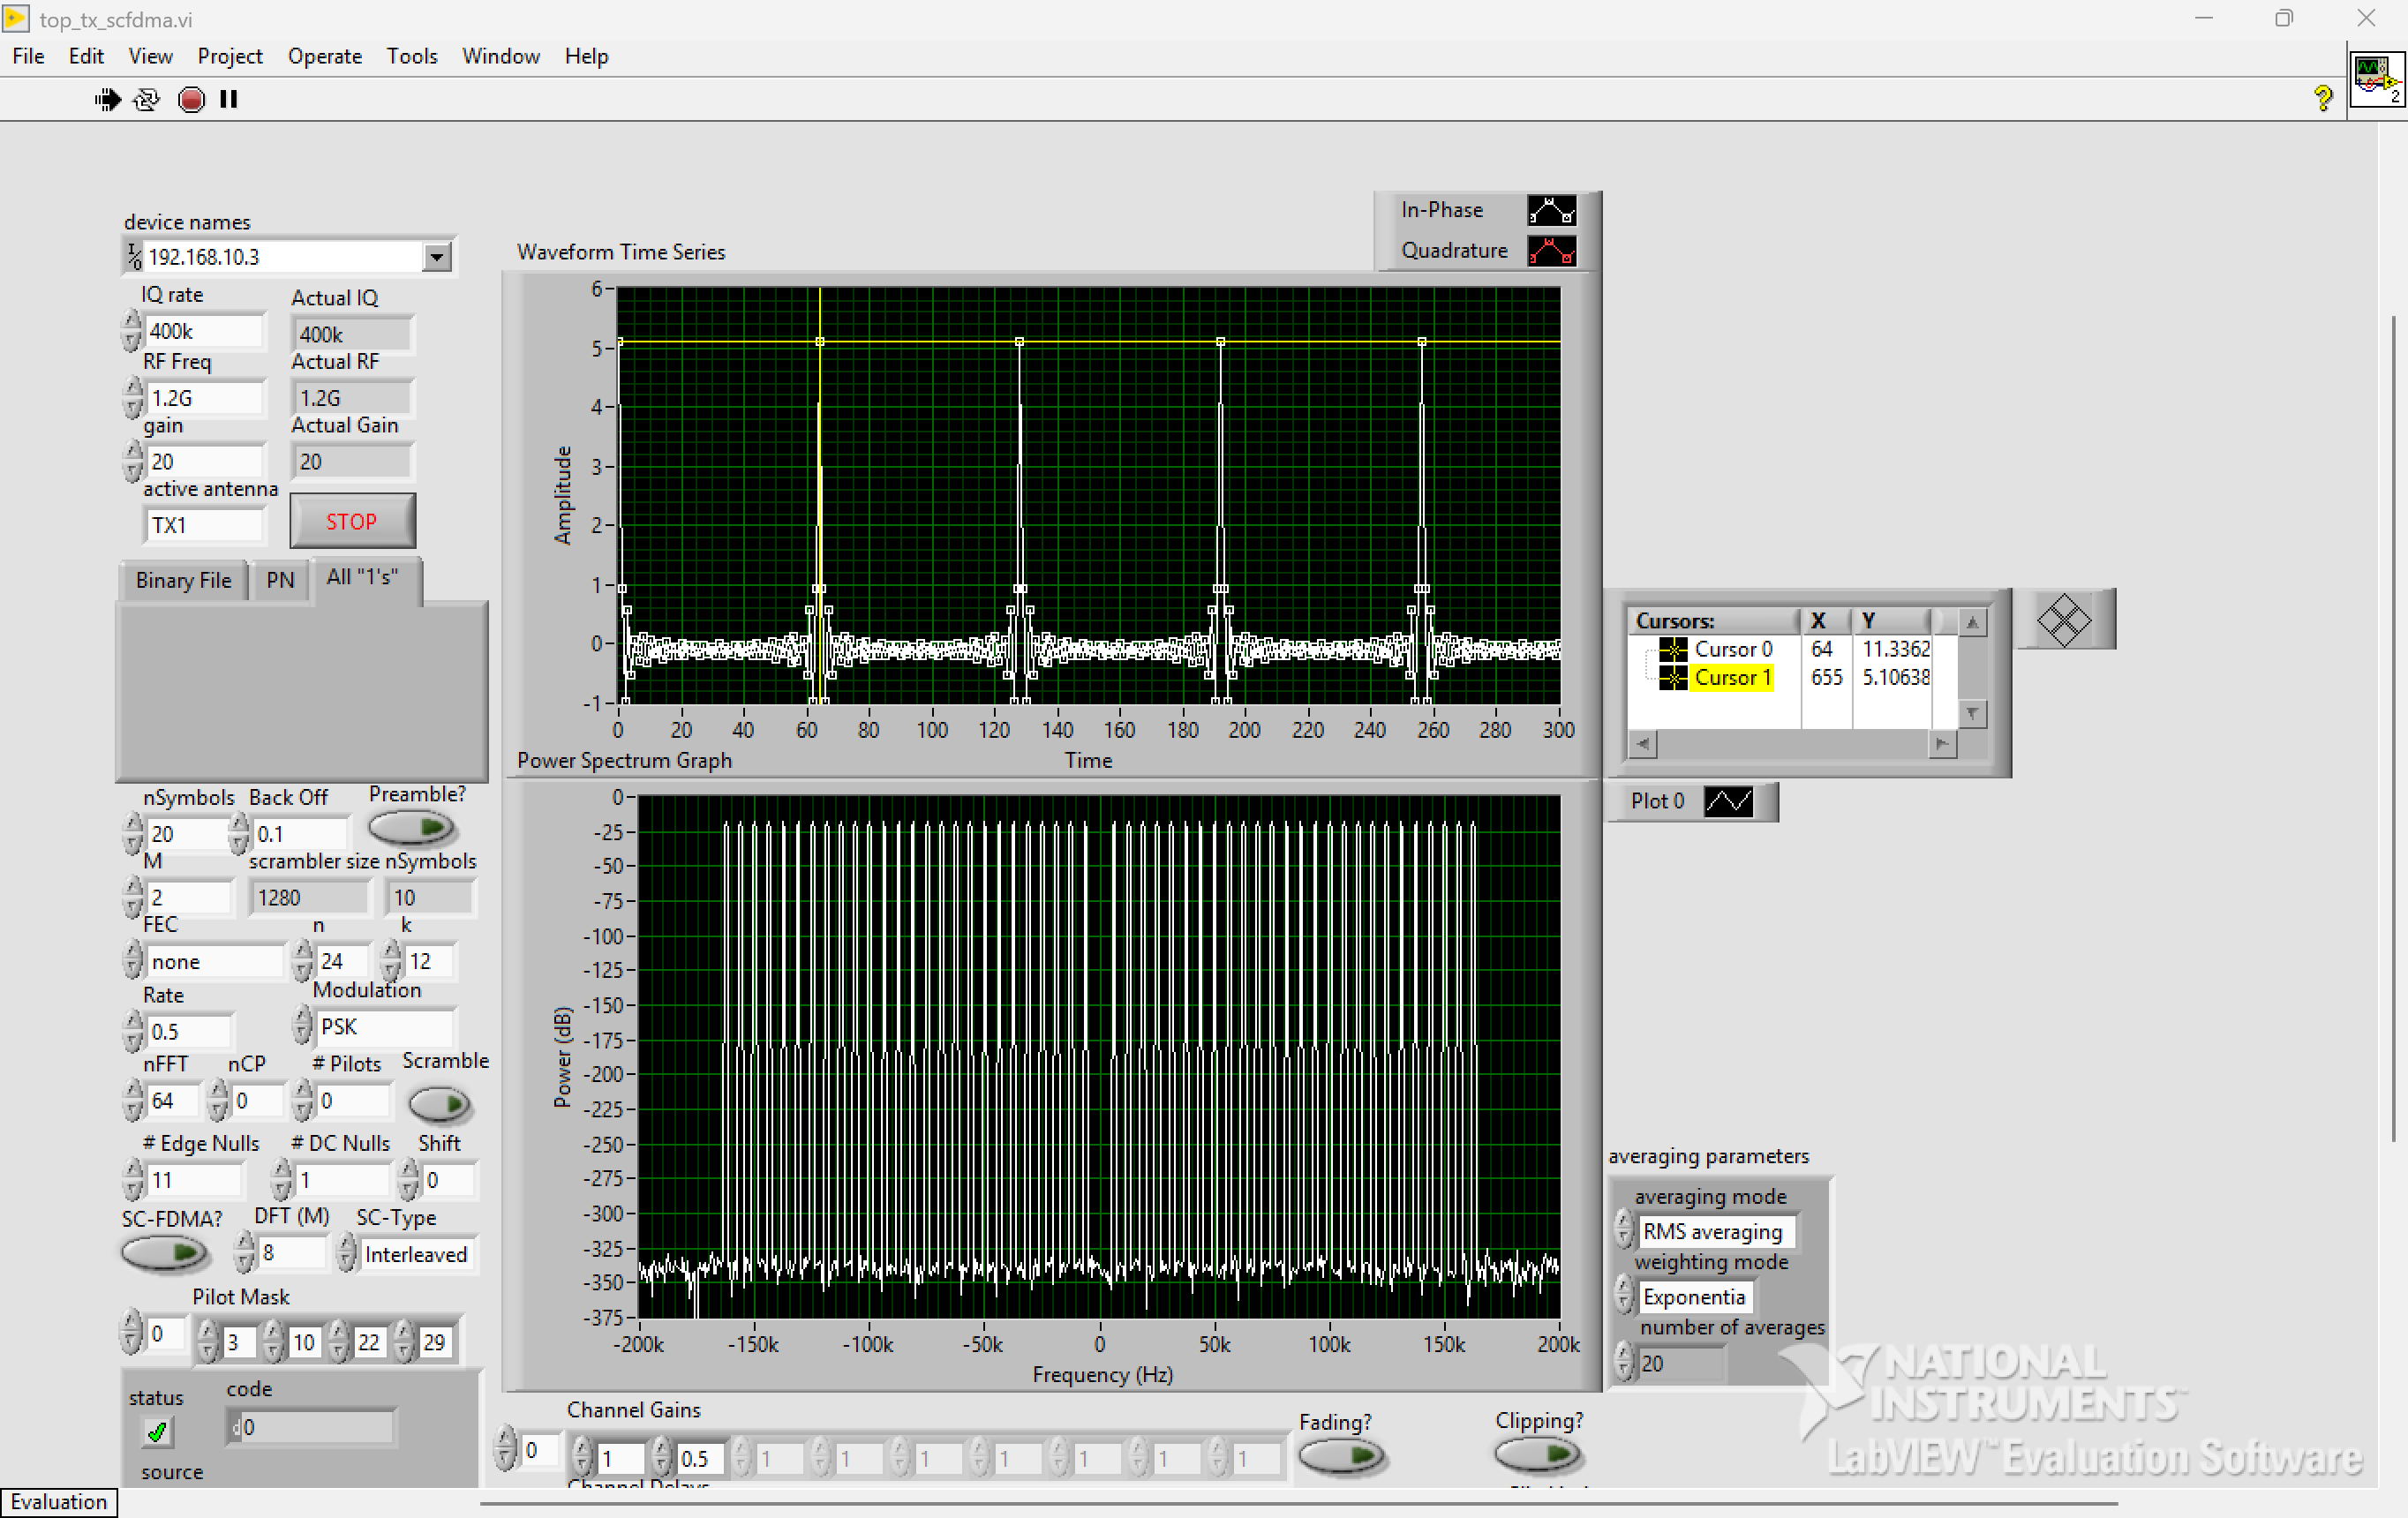
\includegraphics[width=0.7\textwidth]{lab_ss/WES268B_Lab7_Part2-1-8_scramblerOFF_all1s_nFFT-64_edgeNulls-11_dcNull-1_PAPR-7dB_idk.png}
    \caption{Lab 7 - Scrambler OFF, All 1's, FFT size = 64, 802.11g w/ QPSK, PAPR = 7dB}
    %\label{f35}
\end{figure}

% 2.1.9
\subsubsection{ }

\noindent\textbf{Question.}
{
    How does the PAPR change as a function of the number of active subcarriers?
}

\noindent\textbf{Answer.}
{
    The PAPR increases logarithmically as the number of active subcarriers increase. This is because each subcarrier adds constructively 
    to each other, causing rare but large peaks to appear when all subcarriers are peaking.
}

% 2.2
\subsection{SC-FDMA}

% 2.2.1
\subsubsection{ }

% 2.2.2
\subsubsection{ }

% 2.2.3
\subsubsection{ }
\begin{figure}[H]
    \centering
    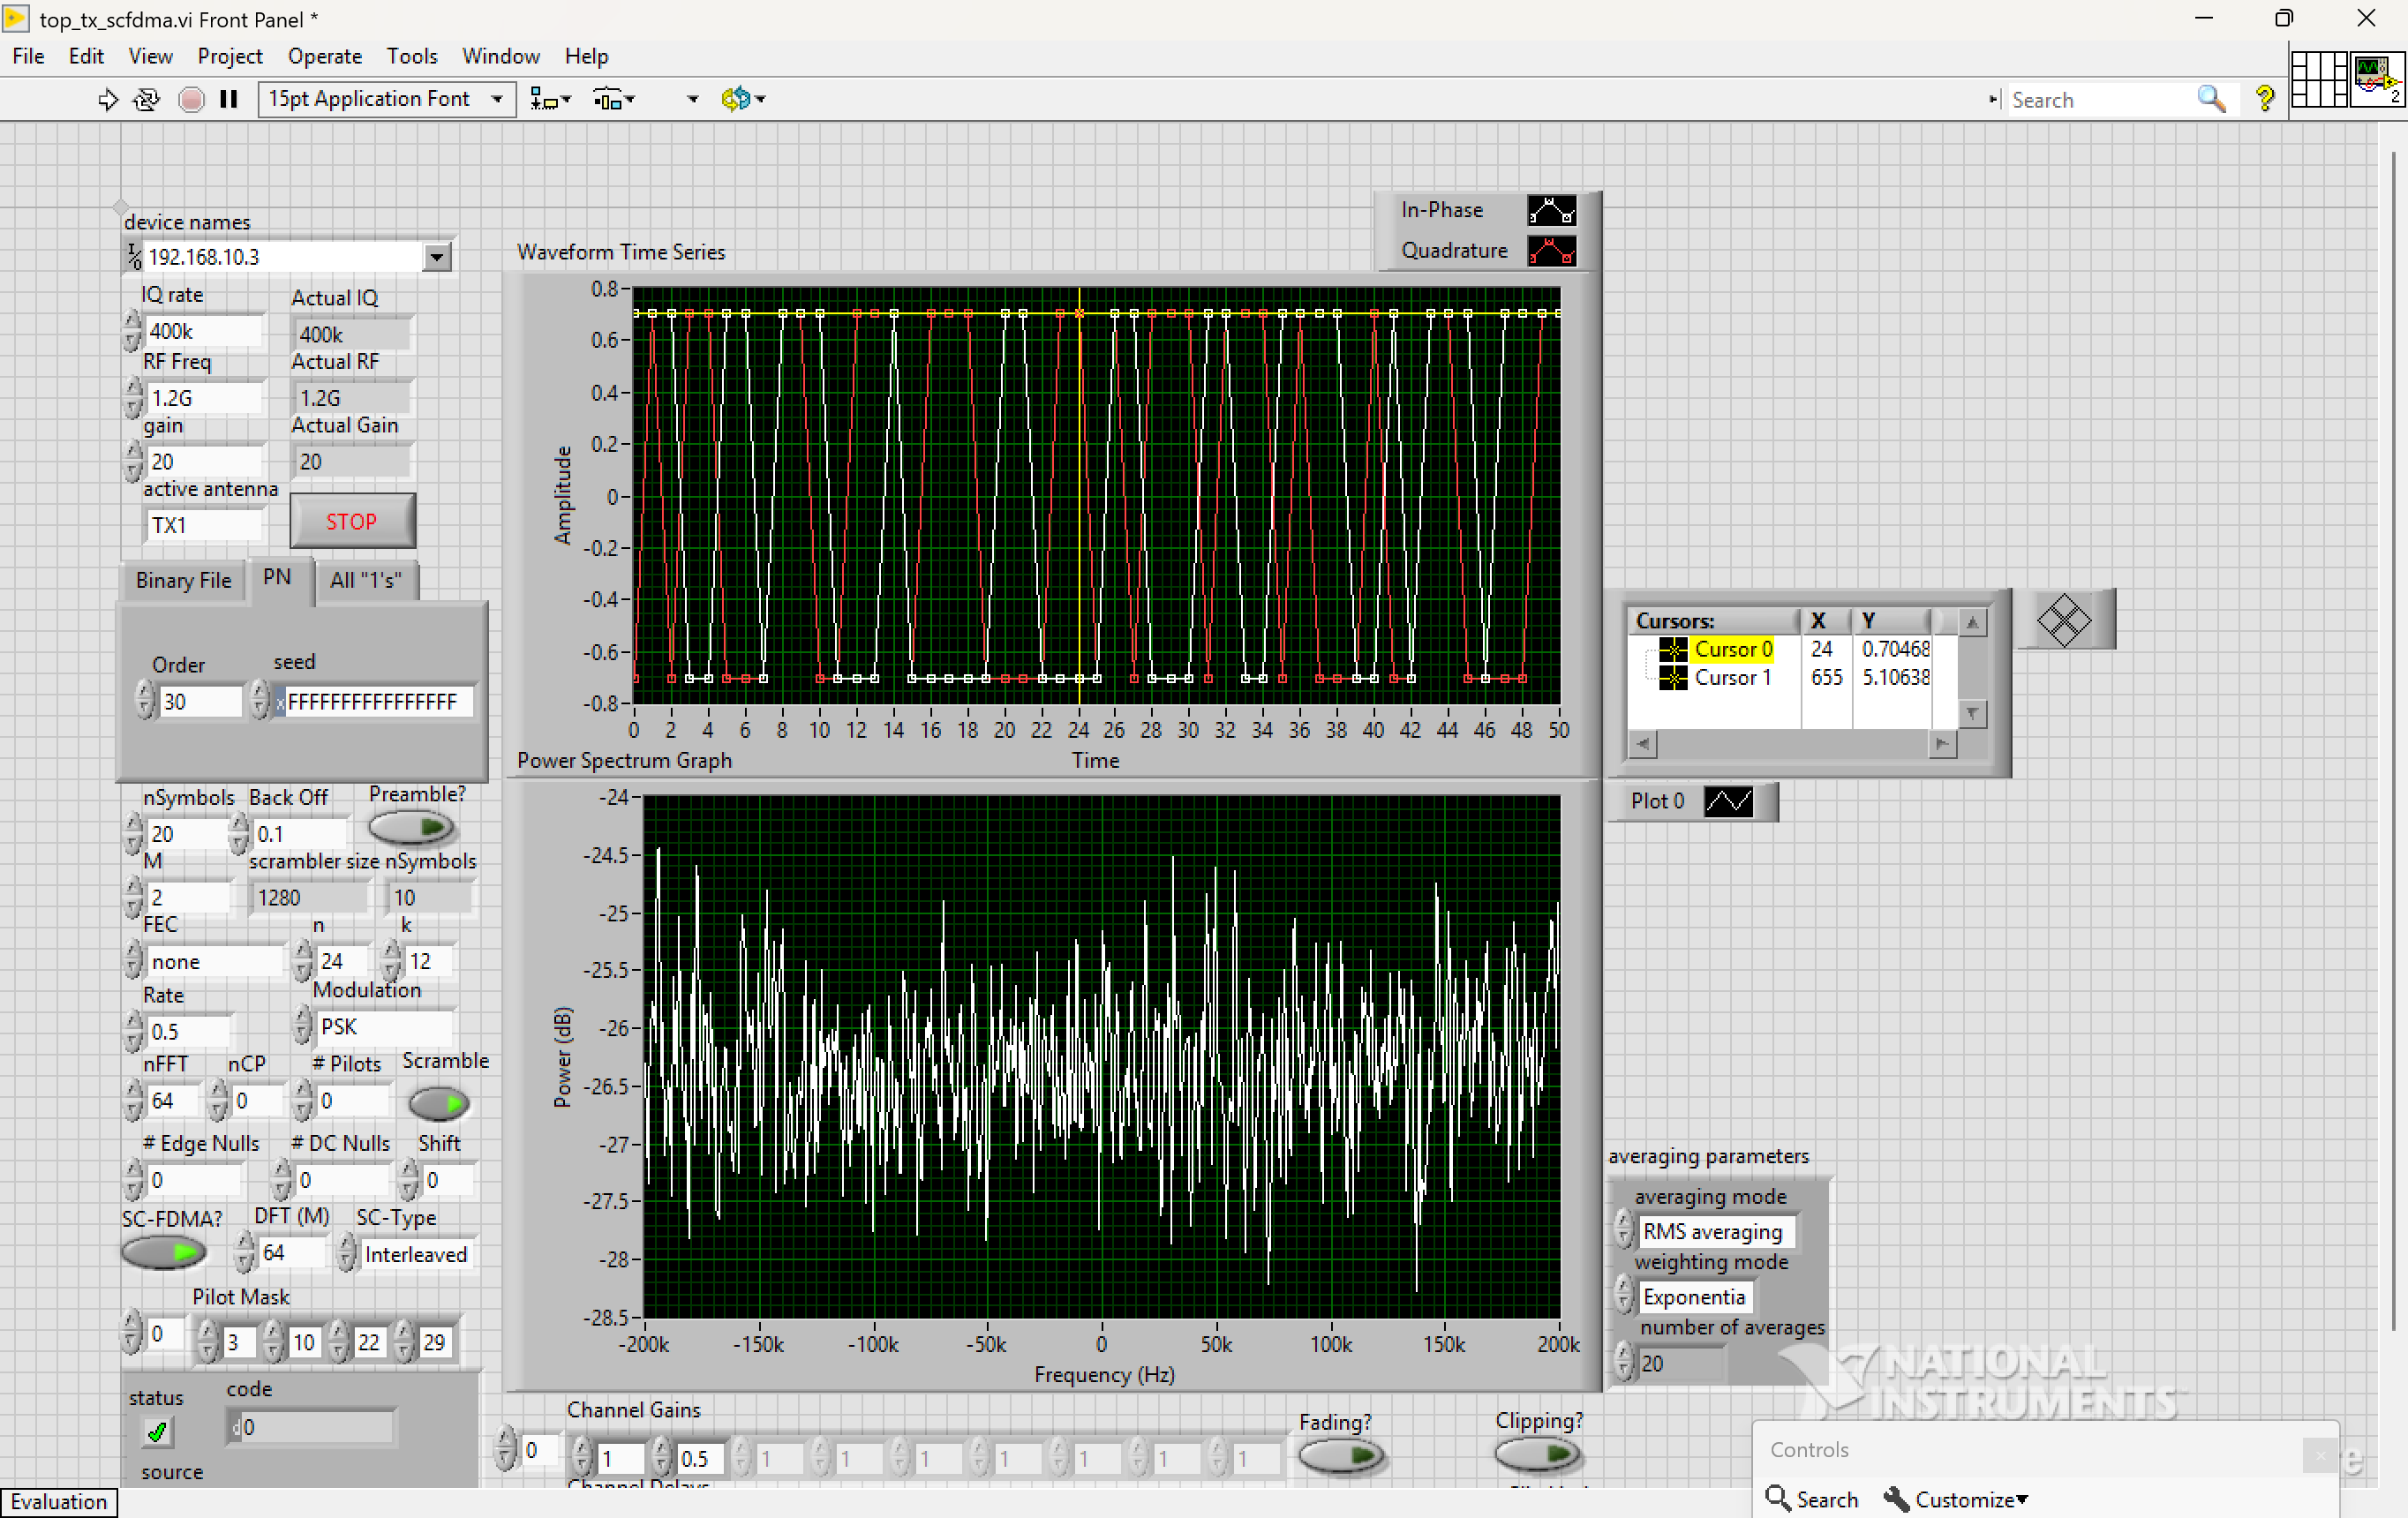
\includegraphics[width=0.7\textwidth]{lab_ss/WES268B_Lab7_Part2-2-3_Tx_PAPR-0dB.png}
    \caption{Lab 7 - Scrambler ON, SC-FDMA, FFT Size = 64, PAPR = 0dB}
    %\label{f36}
\end{figure}

% 2.2.4
\subsubsection{ }

% 2.2.5
\subsubsection{ }
\begin{figure}[H]
    \centering
    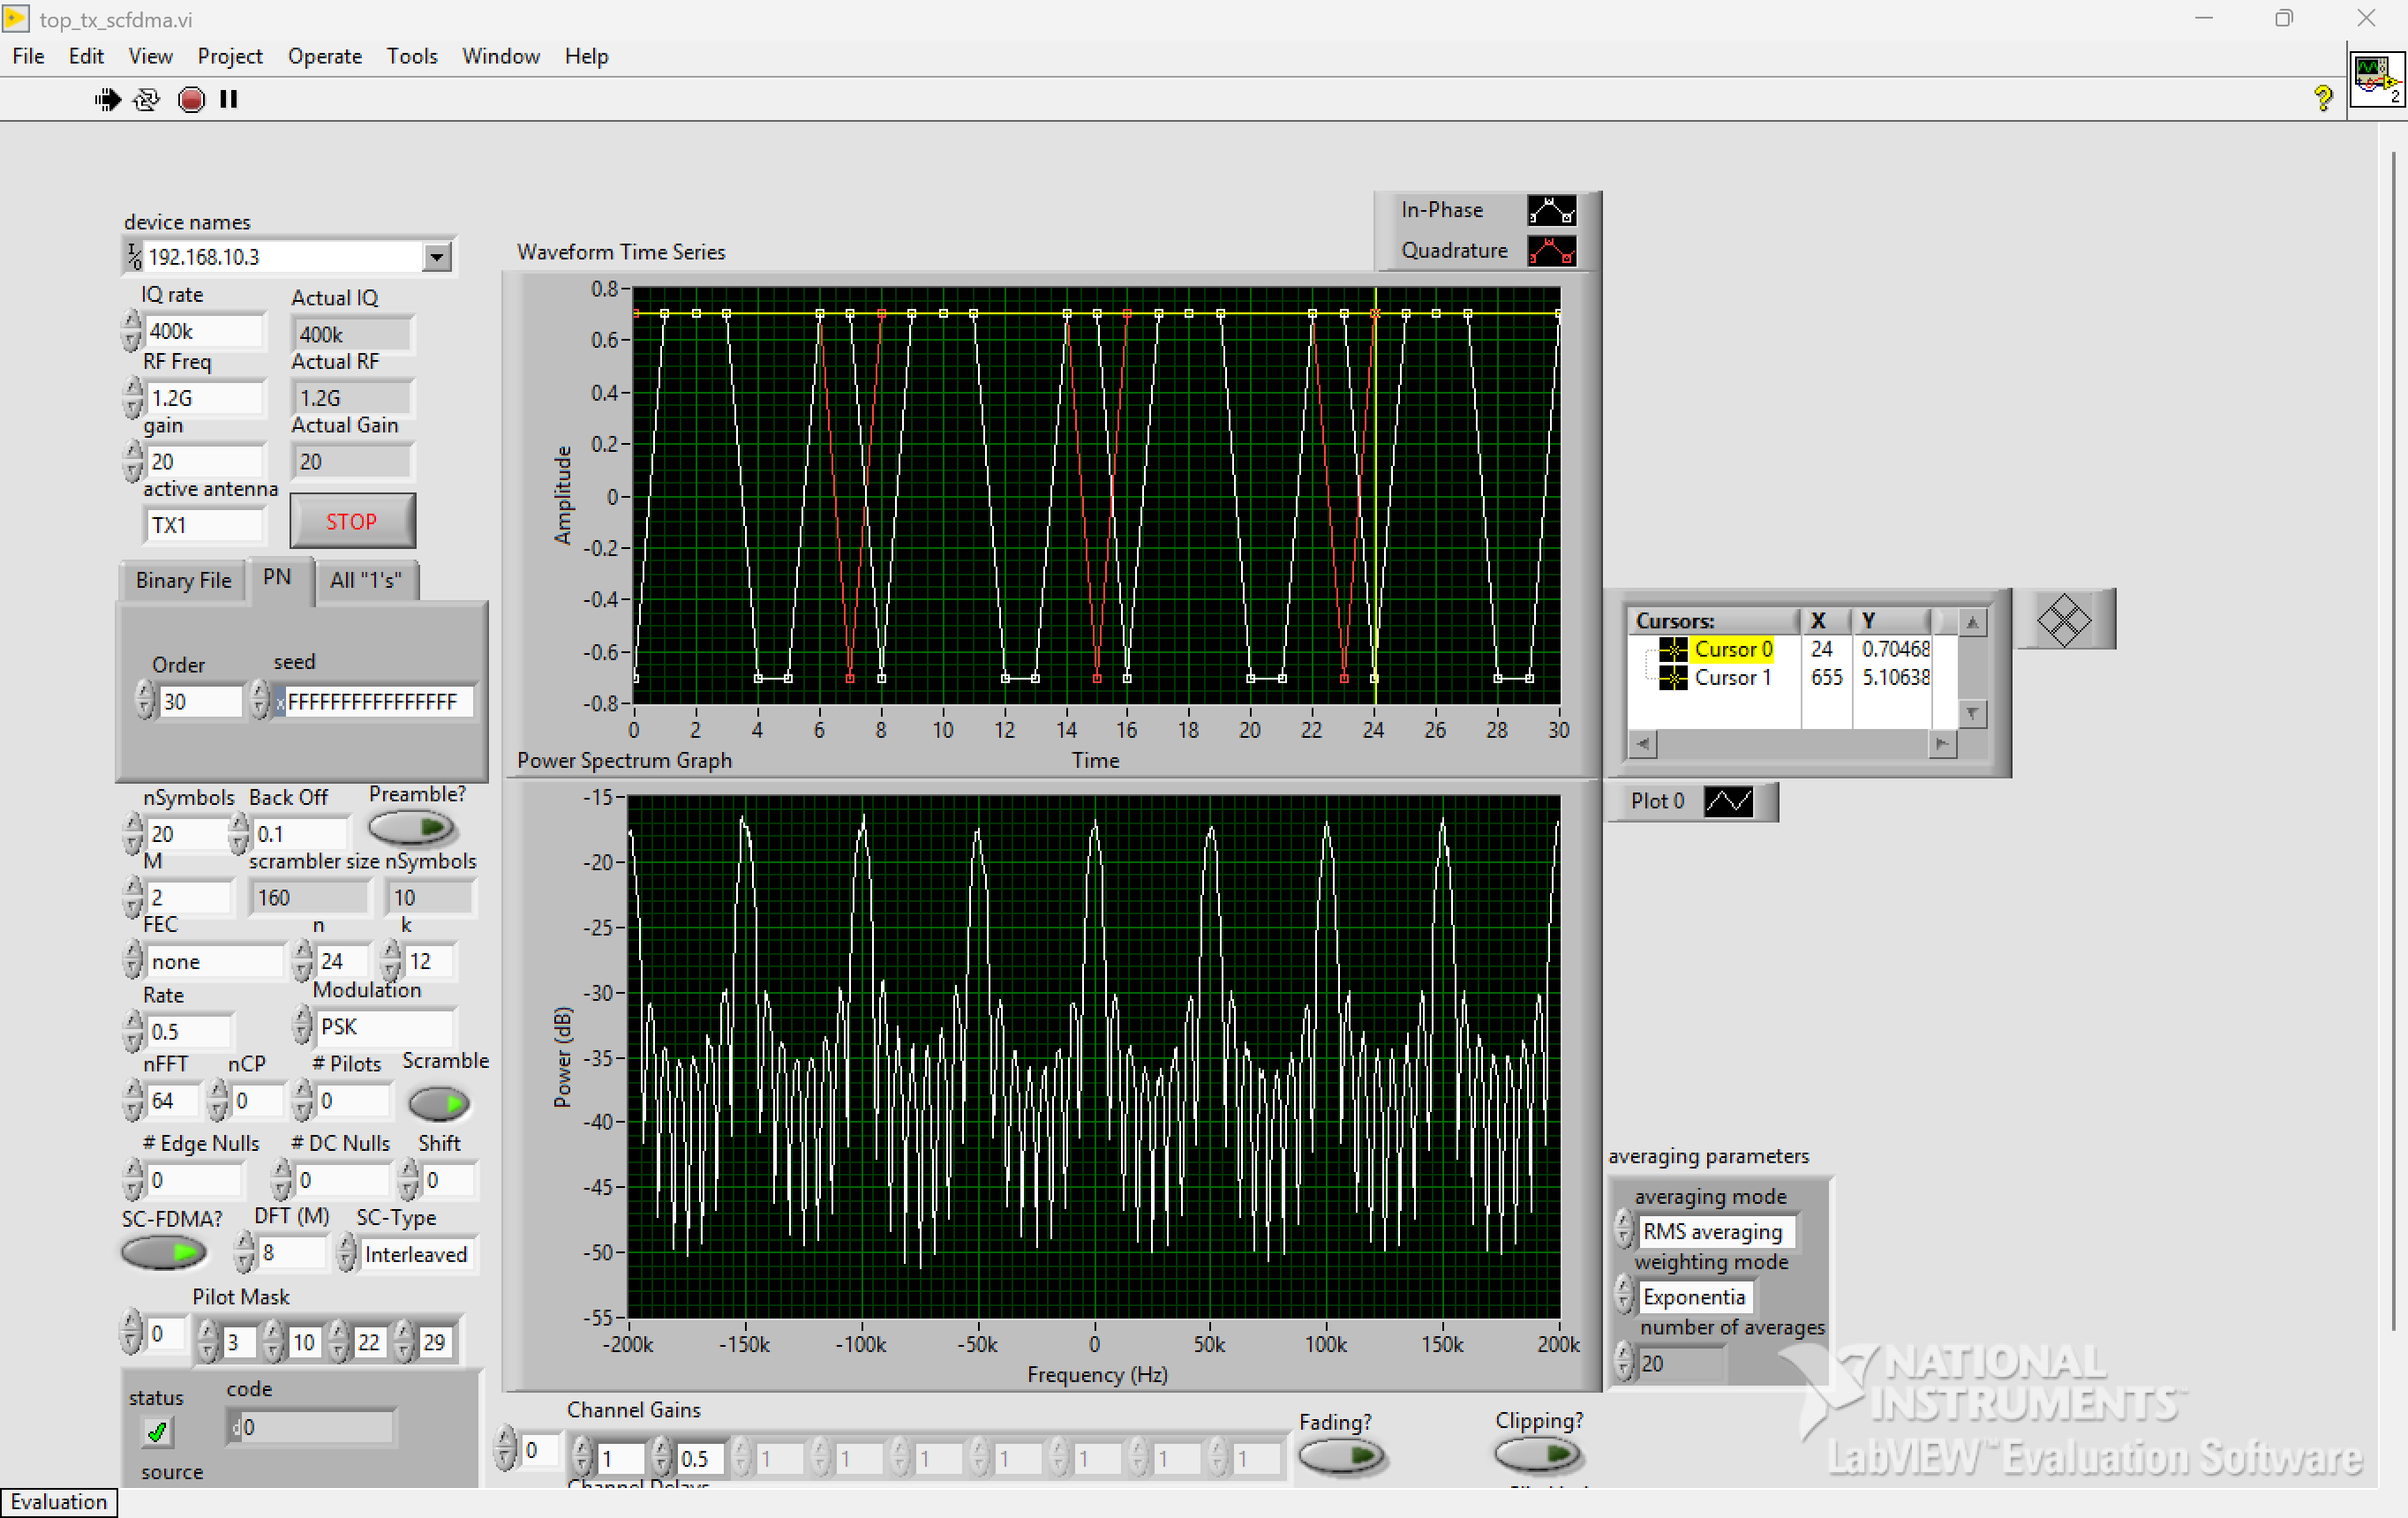
\includegraphics[width=0.7\textwidth]{lab_ss/WES268B_Lab7_Part2-2-5_Tx_DFT-8_PAPR-0dB.png}
    \caption{Lab 7 - SC-FDMA, SC-Type Interleaved, DFT Size = 8, PAPR = 0dB}
    %\label{f37}
\end{figure}

\begin{figure}[H]
    \centering
    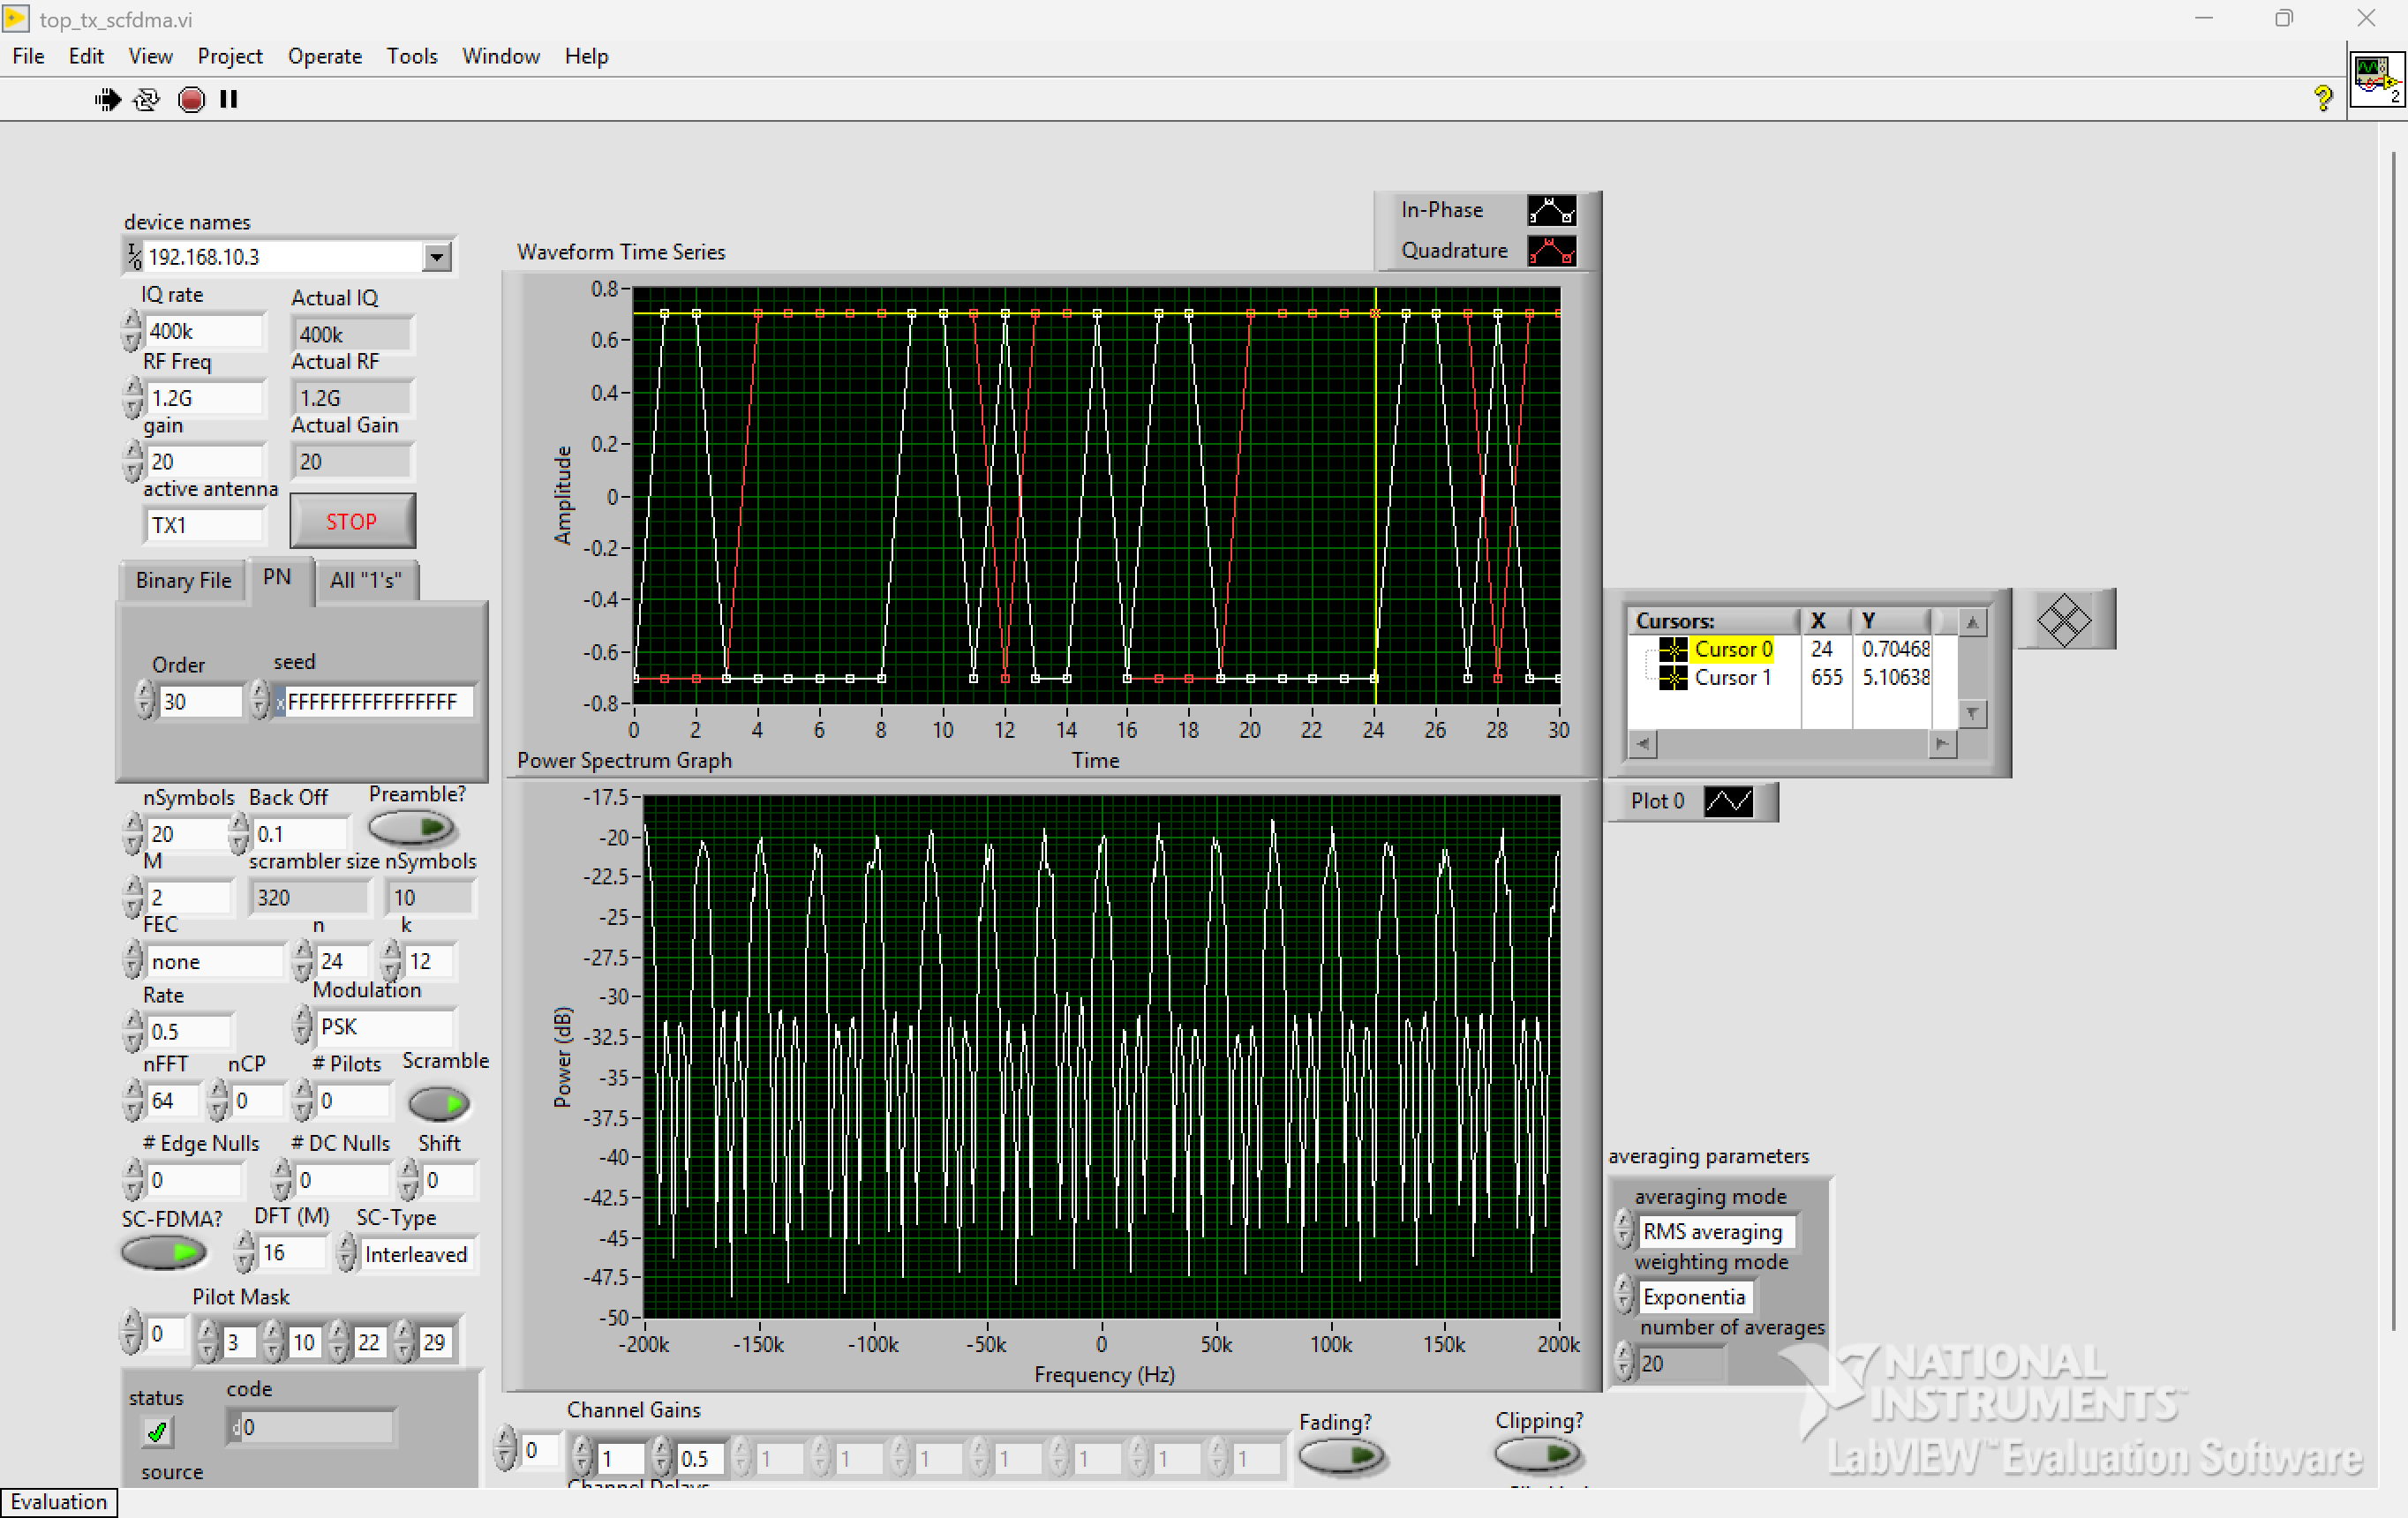
\includegraphics[width=0.7\textwidth]{lab_ss/WES268B_Lab7_Part2-2-5_Tx_DFT-16_PAPR-0dB.png}
    \caption{Lab 7 - SC-FDMA, SC-Type Interleaved, DFT Size = 16, PAPR = 0dB}
    %\label{f38}
\end{figure}

\begin{figure}[H]
    \centering
    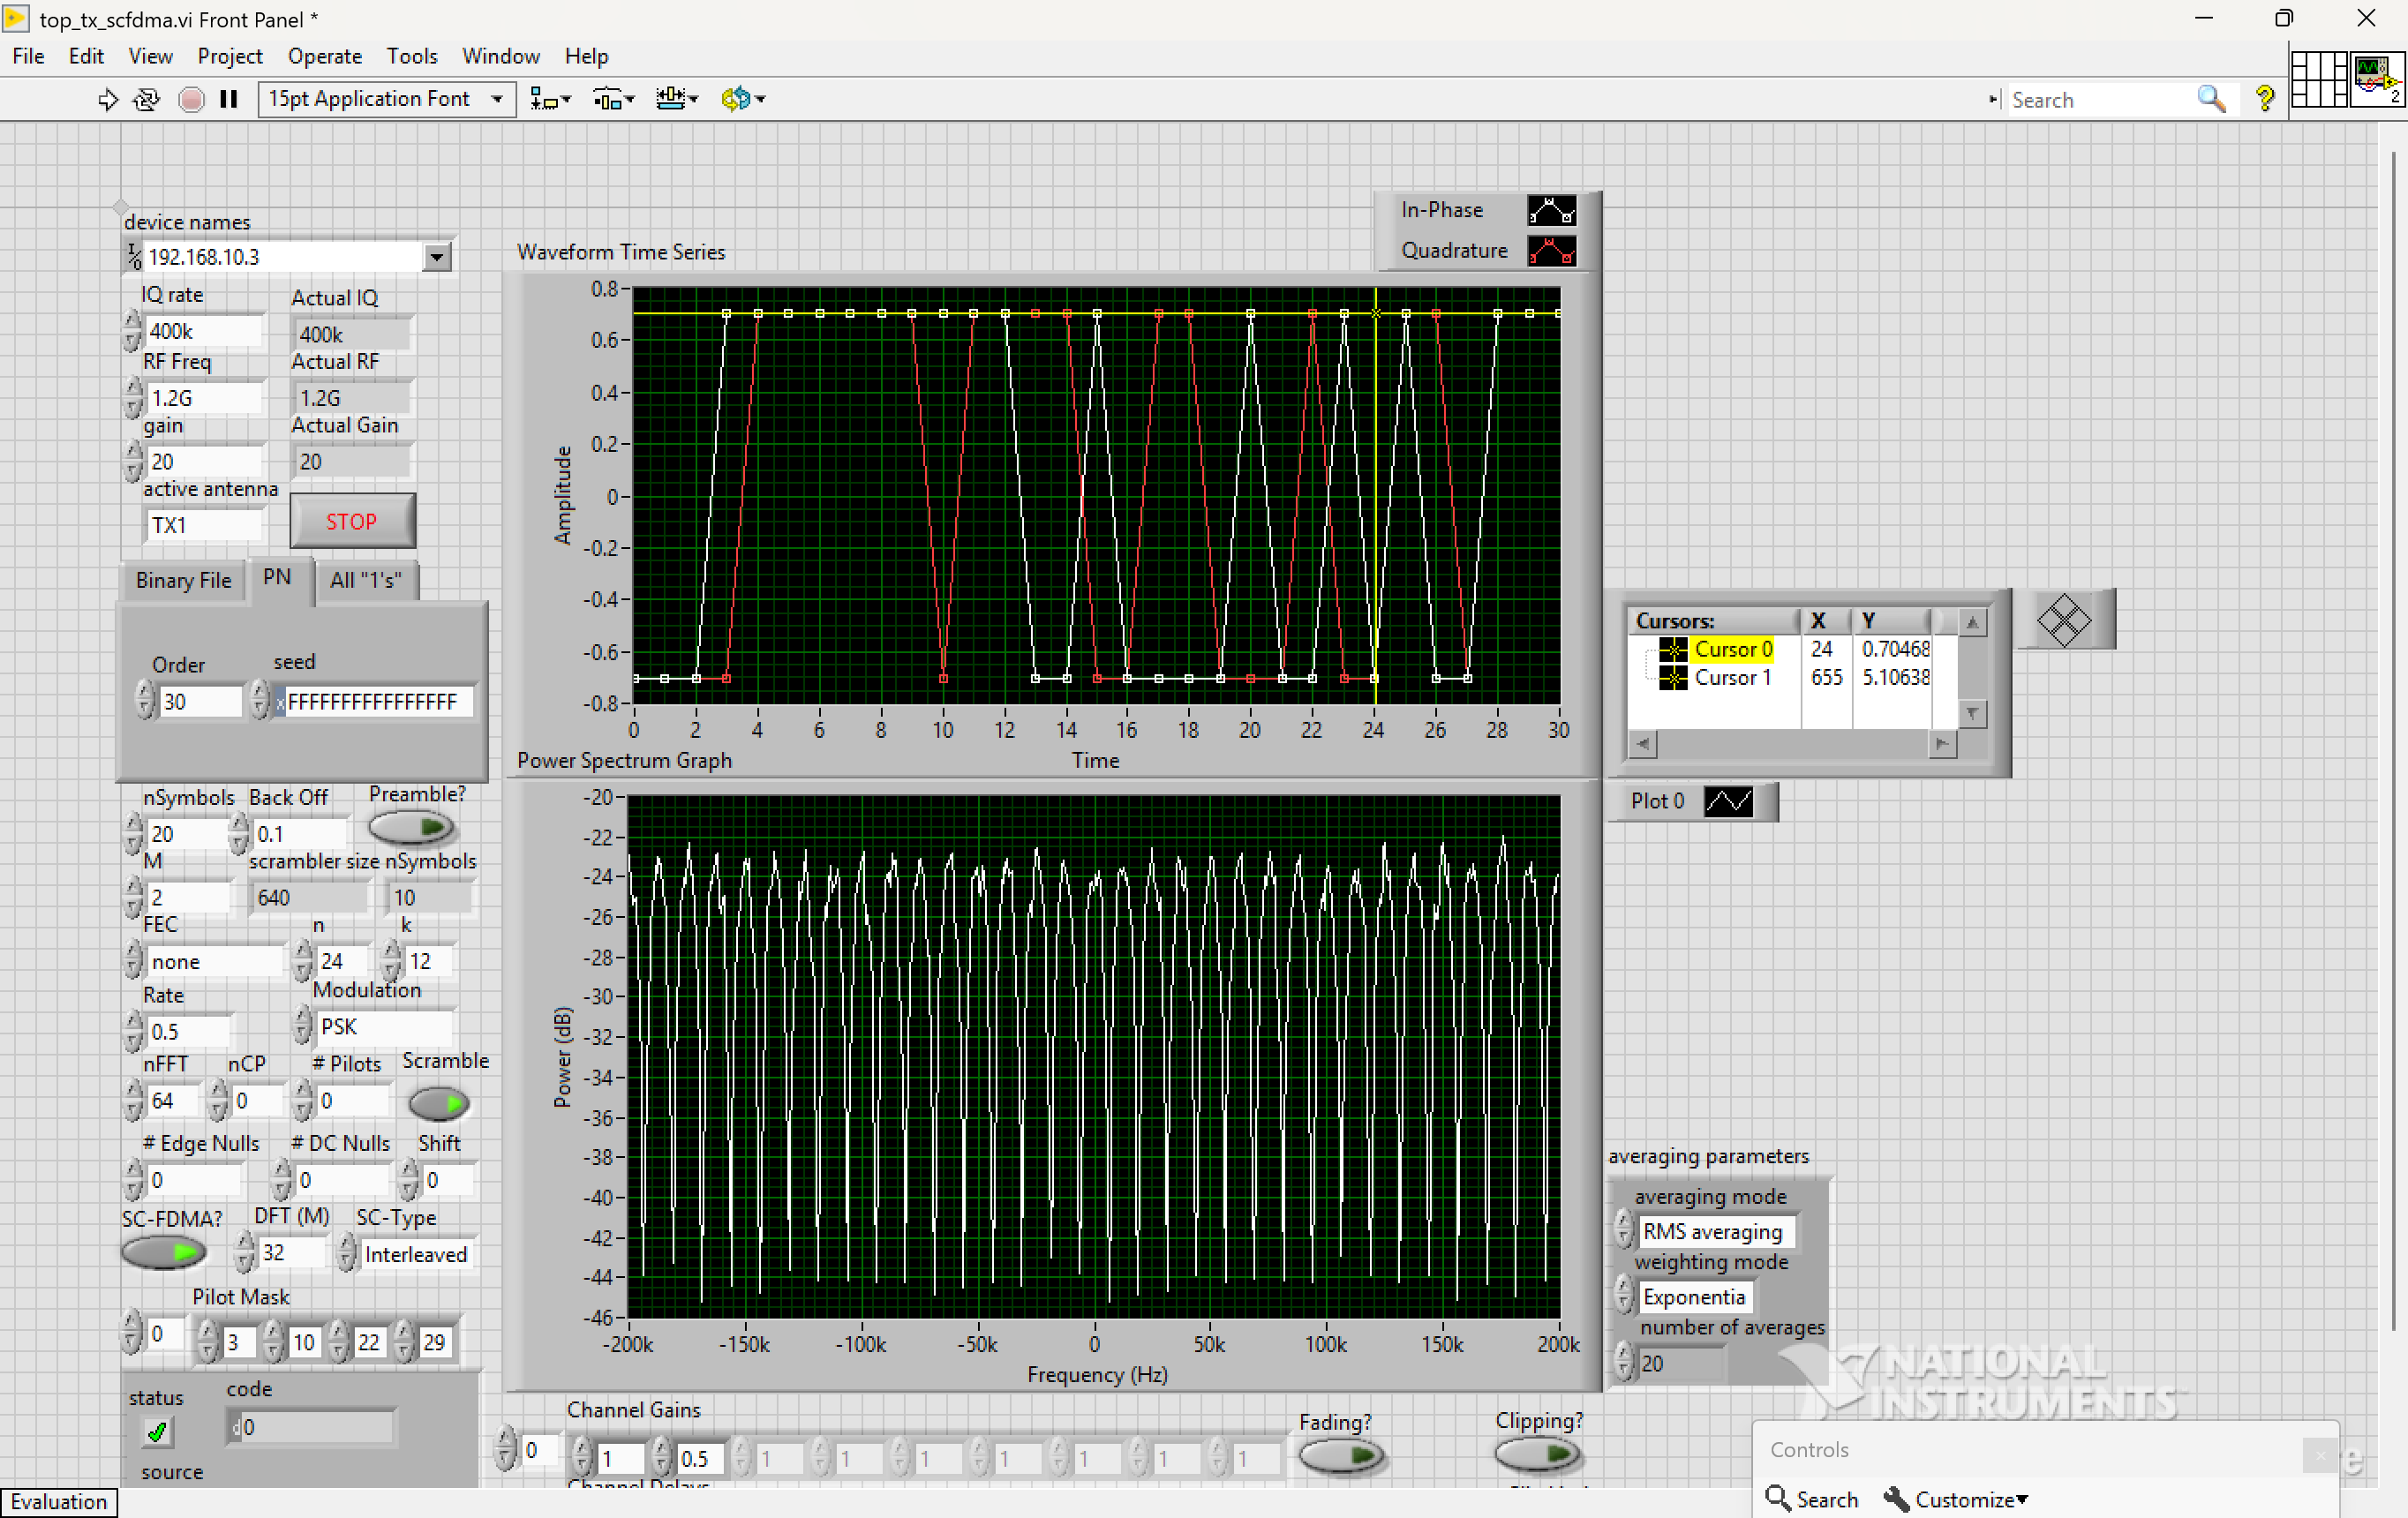
\includegraphics[width=0.7\textwidth]{lab_ss/WES268B_Lab7_Part2-2-5_Tx_DFT-32_PAPR-0dB.png}
    \caption{Lab 7 - SC-FDMA, SC-Type Interleaved, DFT Size = 32, PAPR = 0dB}
    %\label{f39}
\end{figure}
{
    When DFT = nFFT, the waveform acts as a single carrier and has the lowest PAPR. When the DFT is reduced,
    the waveform becomes more OFDM-like and the PAPR increases.
}

% 2.2.6
\subsubsection{ }
\begin{figure}[H]
    \centering
    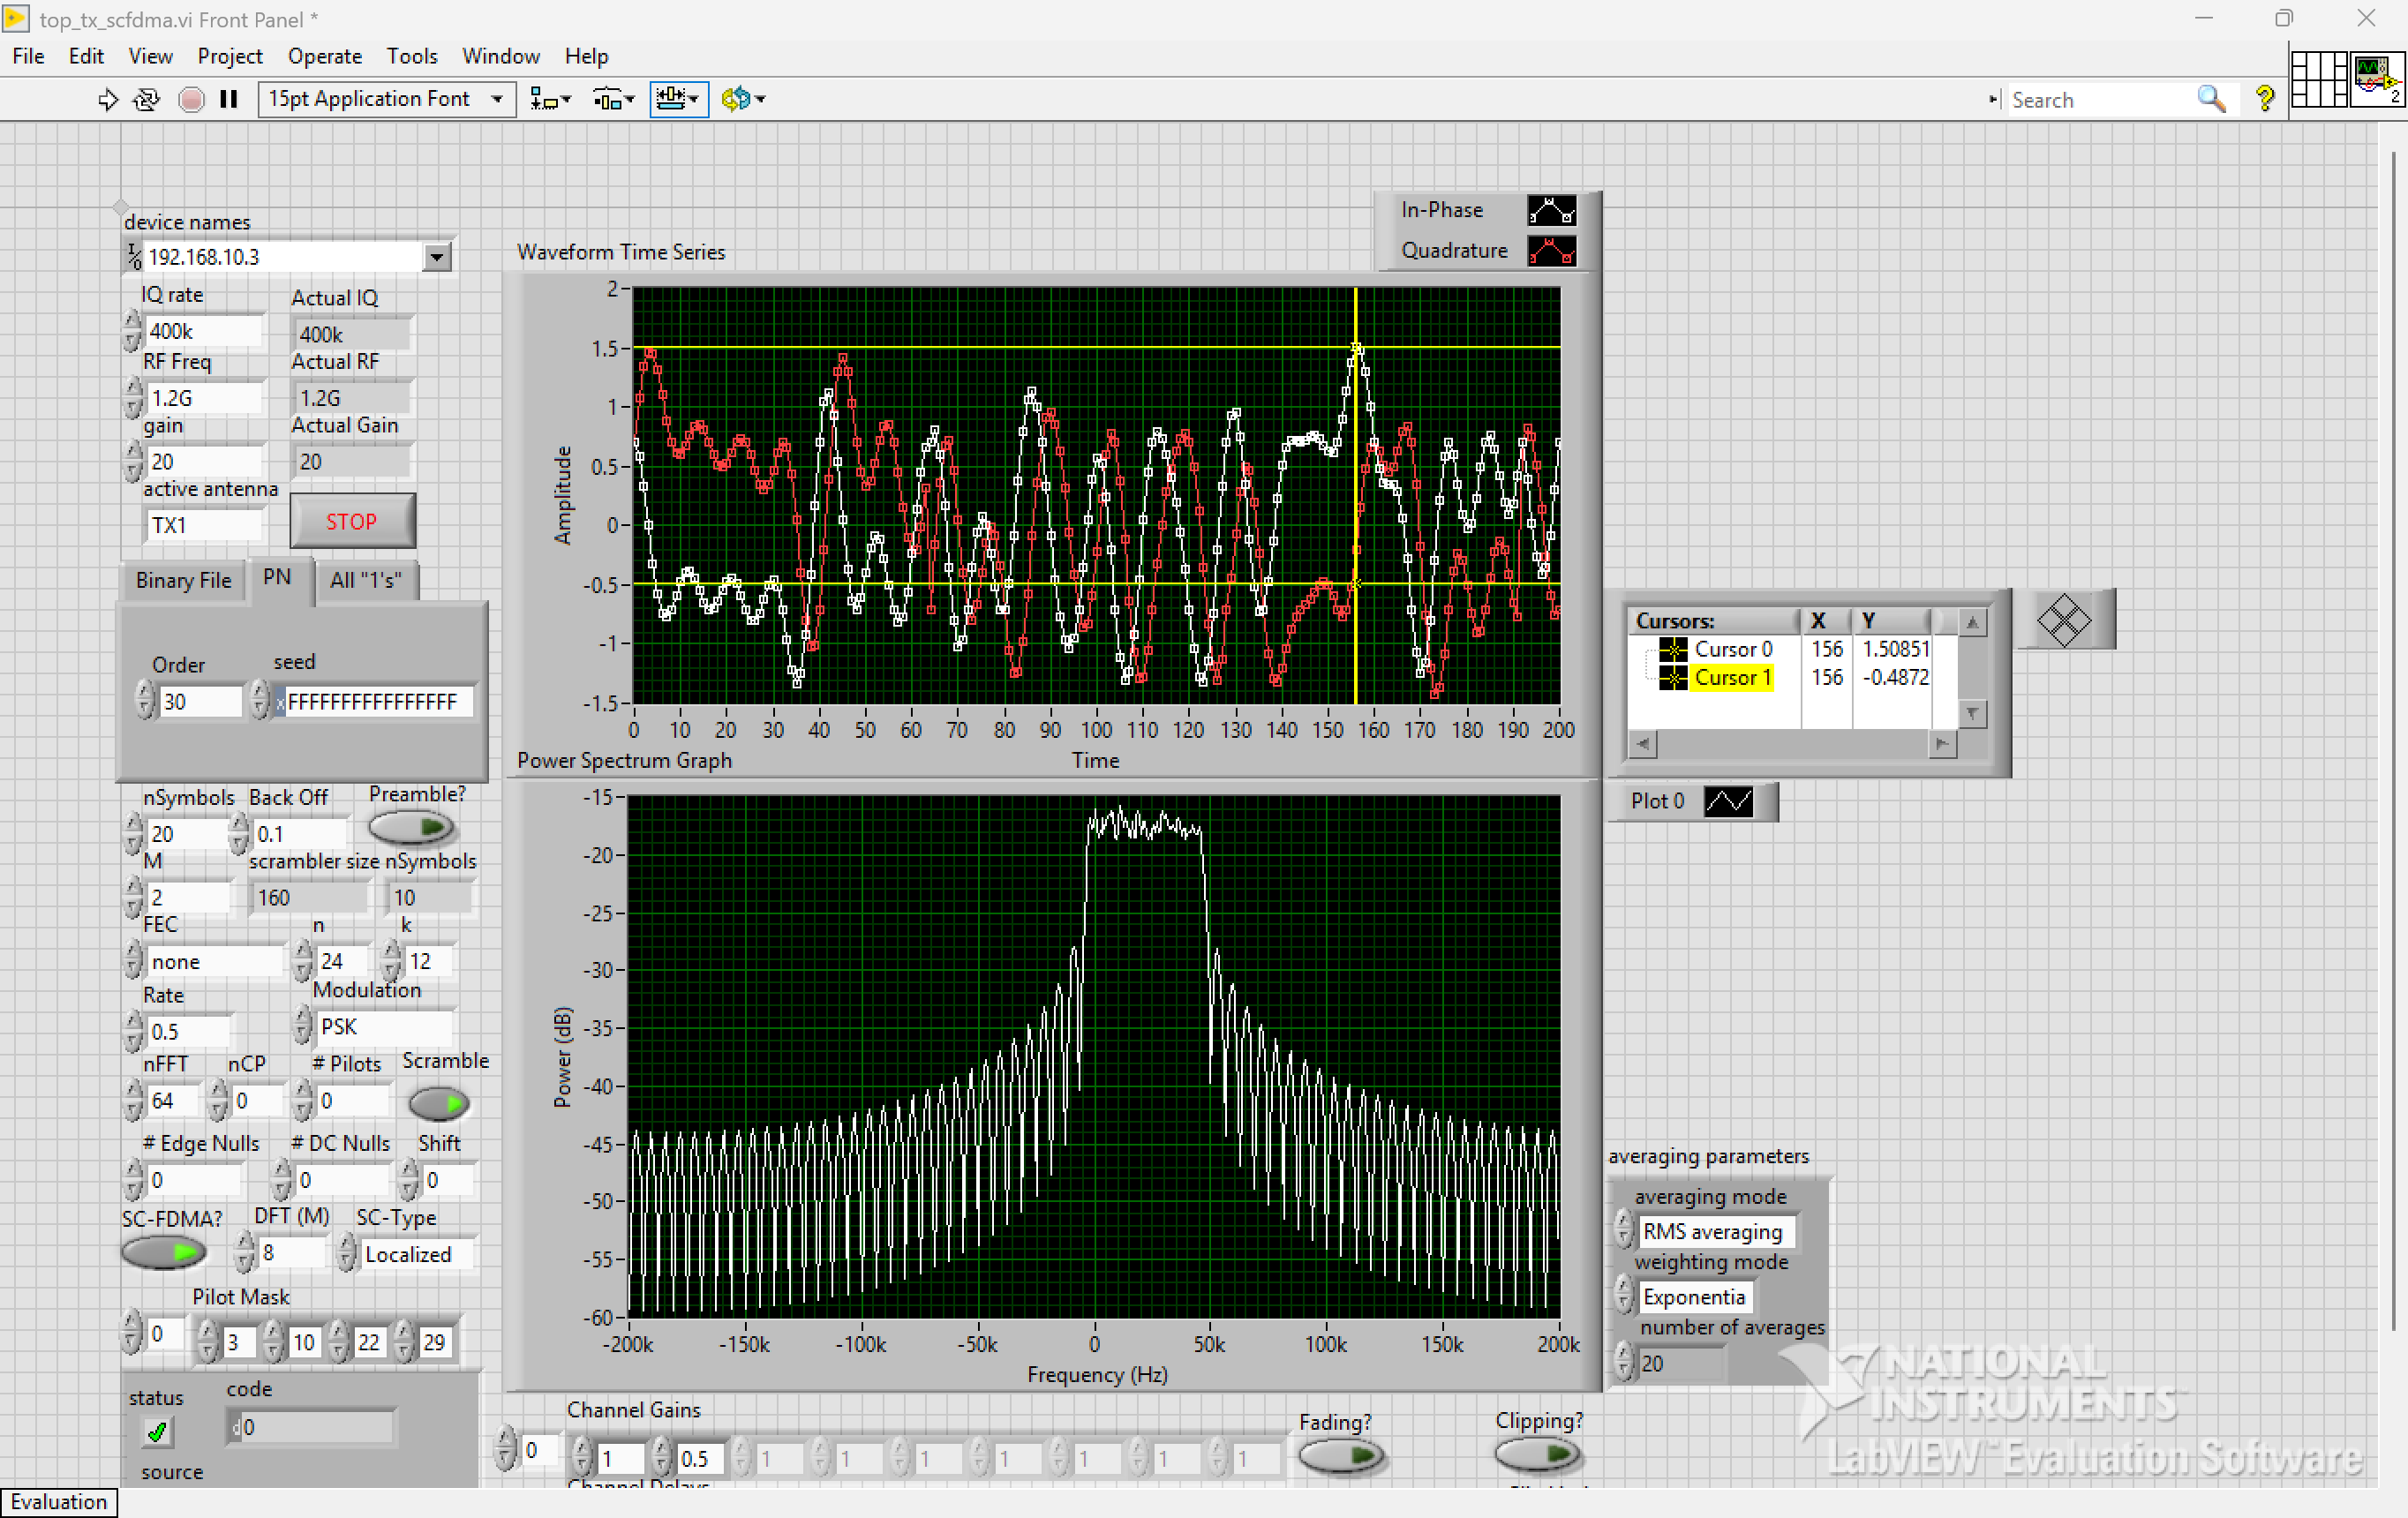
\includegraphics[width=0.7\textwidth]{lab_ss/WES268B_Lab7_Part2-2-6_Tx_Localized_DFT-8_PAPR-4dB_idk.png}
    \caption{Lab 7 - SC-FDMA, SC-Type Localized, DFT Size = 8, PAPR = 4dB}
    %\label{f40}
\end{figure}

\begin{figure}[H]
    \centering
    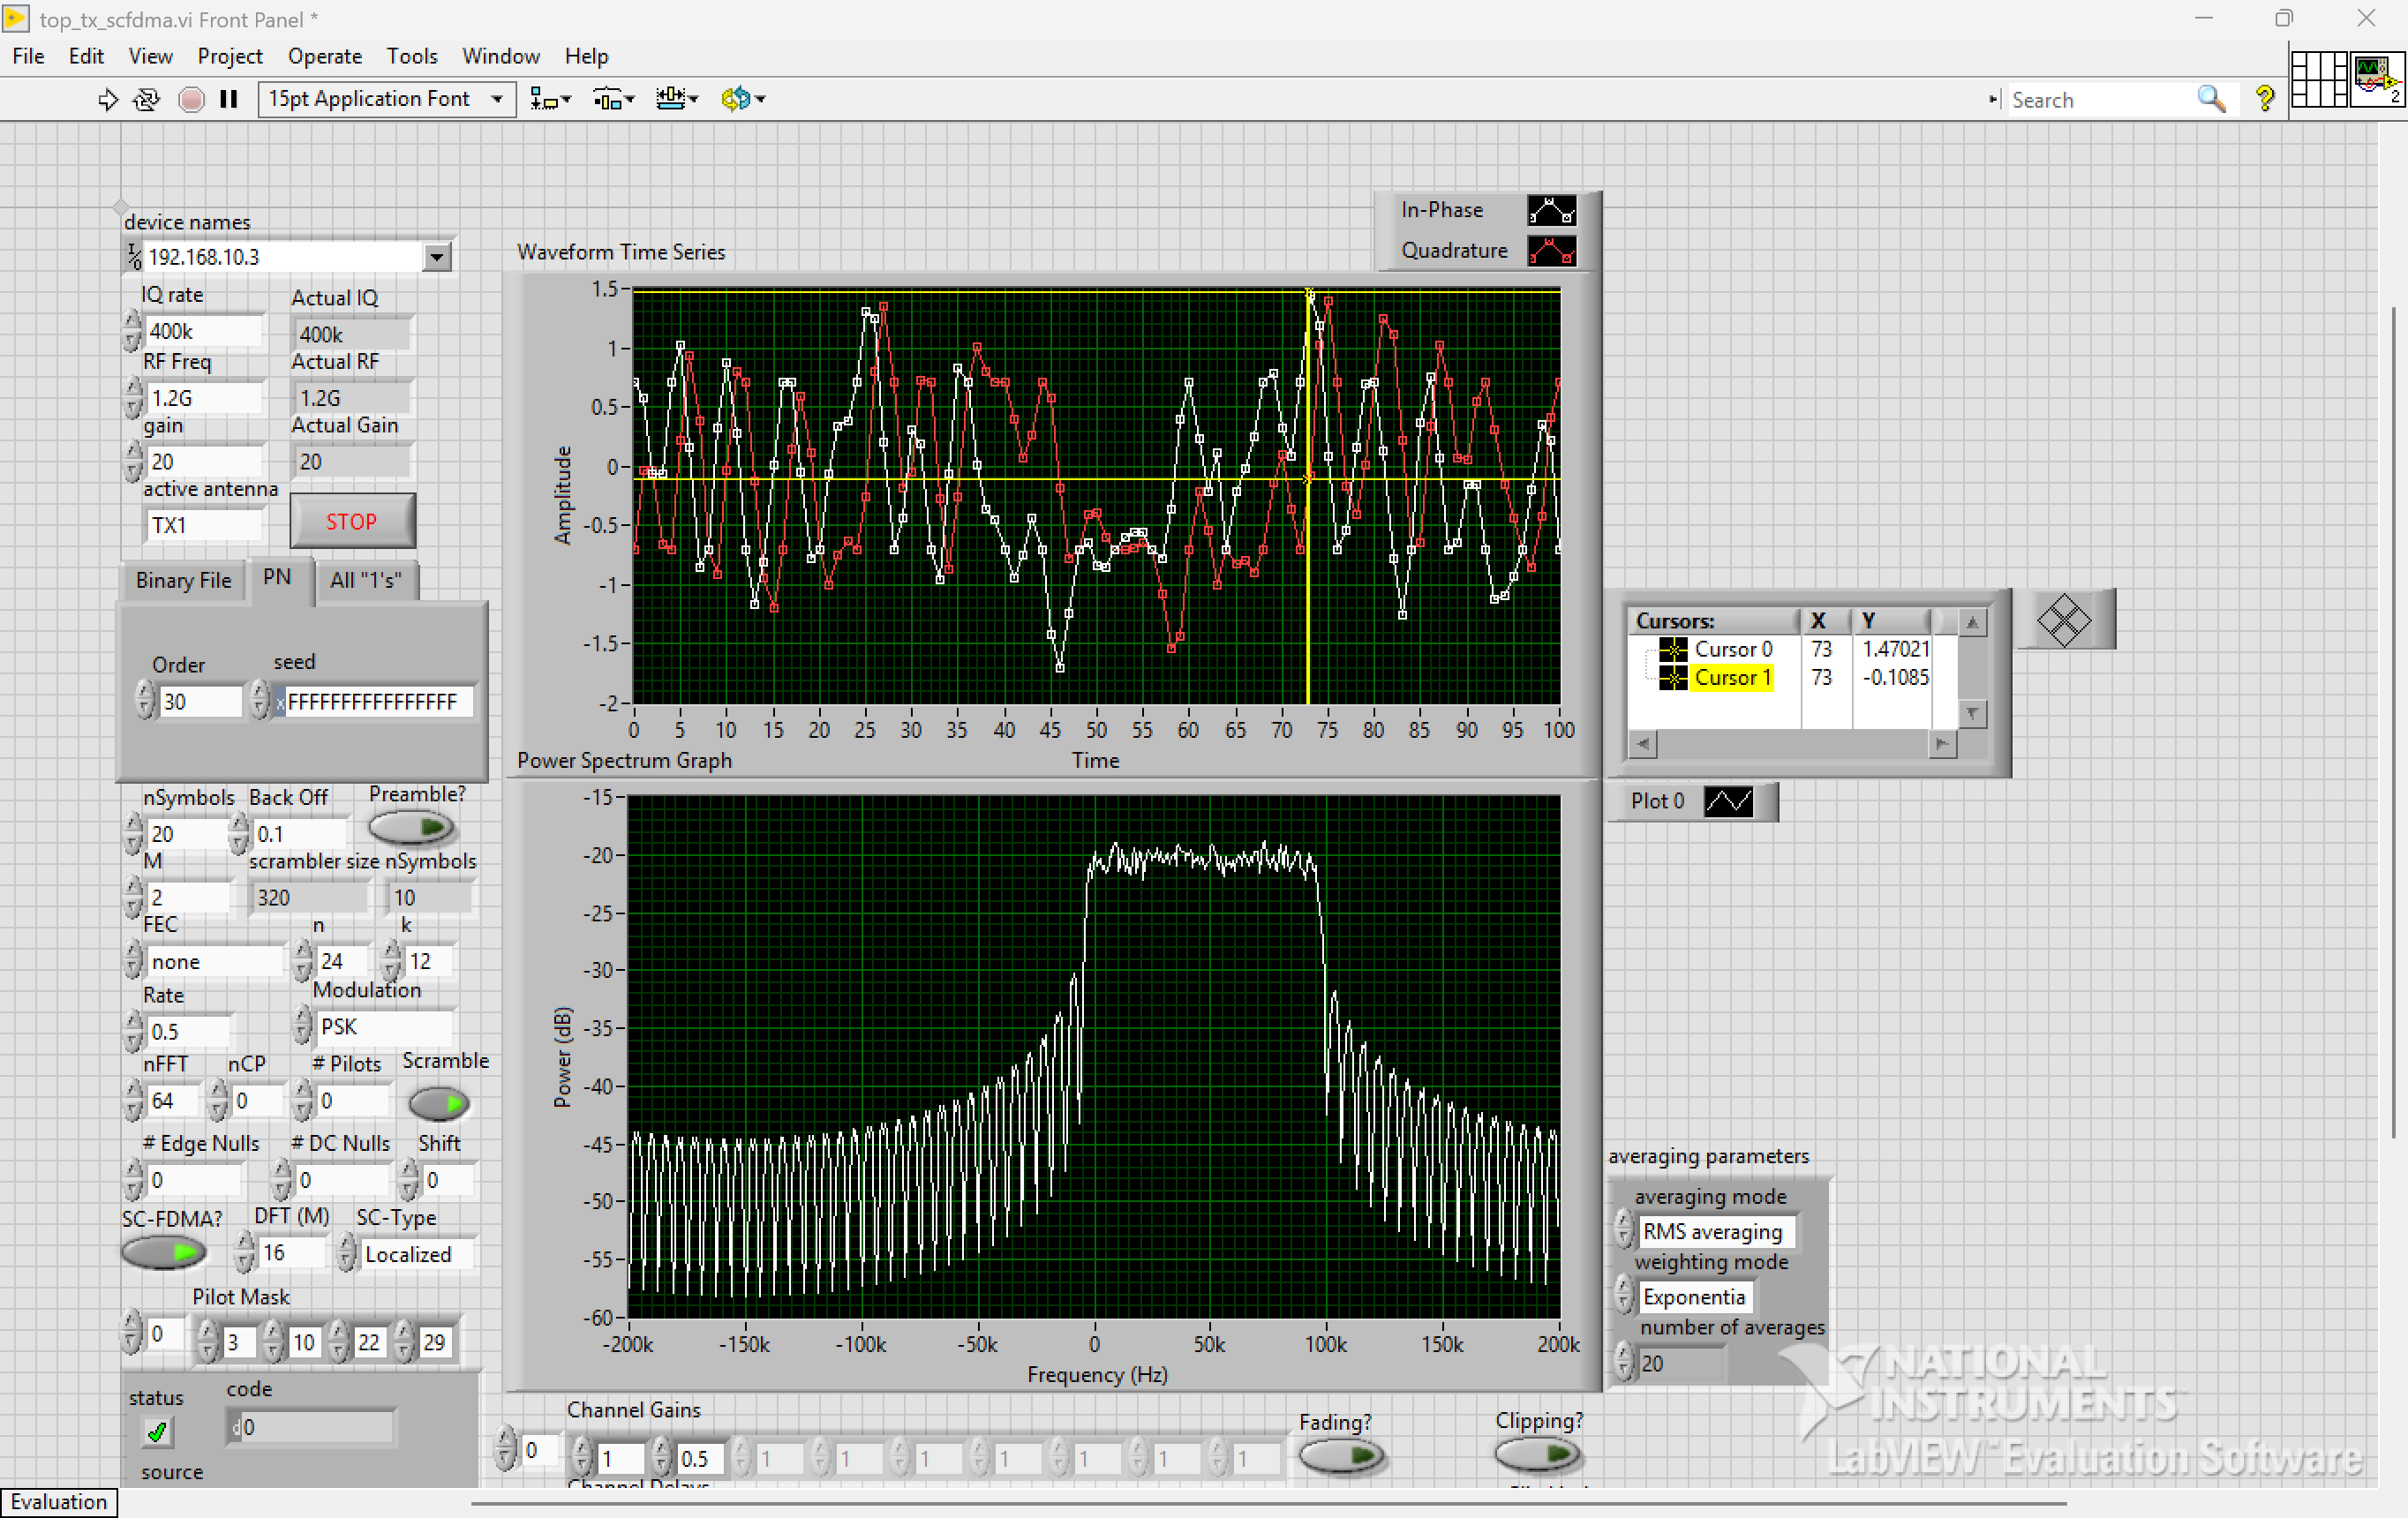
\includegraphics[width=0.7\textwidth]{lab_ss/WES268B_Lab7_Part2-2-6_Tx_Localized_DFT-16_PAPR-3p37dB_idk.png}
    \caption{Lab 7 - SC-FDMA, SC-Type Localized, DFT Size = 16, PAPR = 3.37dB}
    %\label{f41}
\end{figure}

\begin{figure}[H]
    \centering
    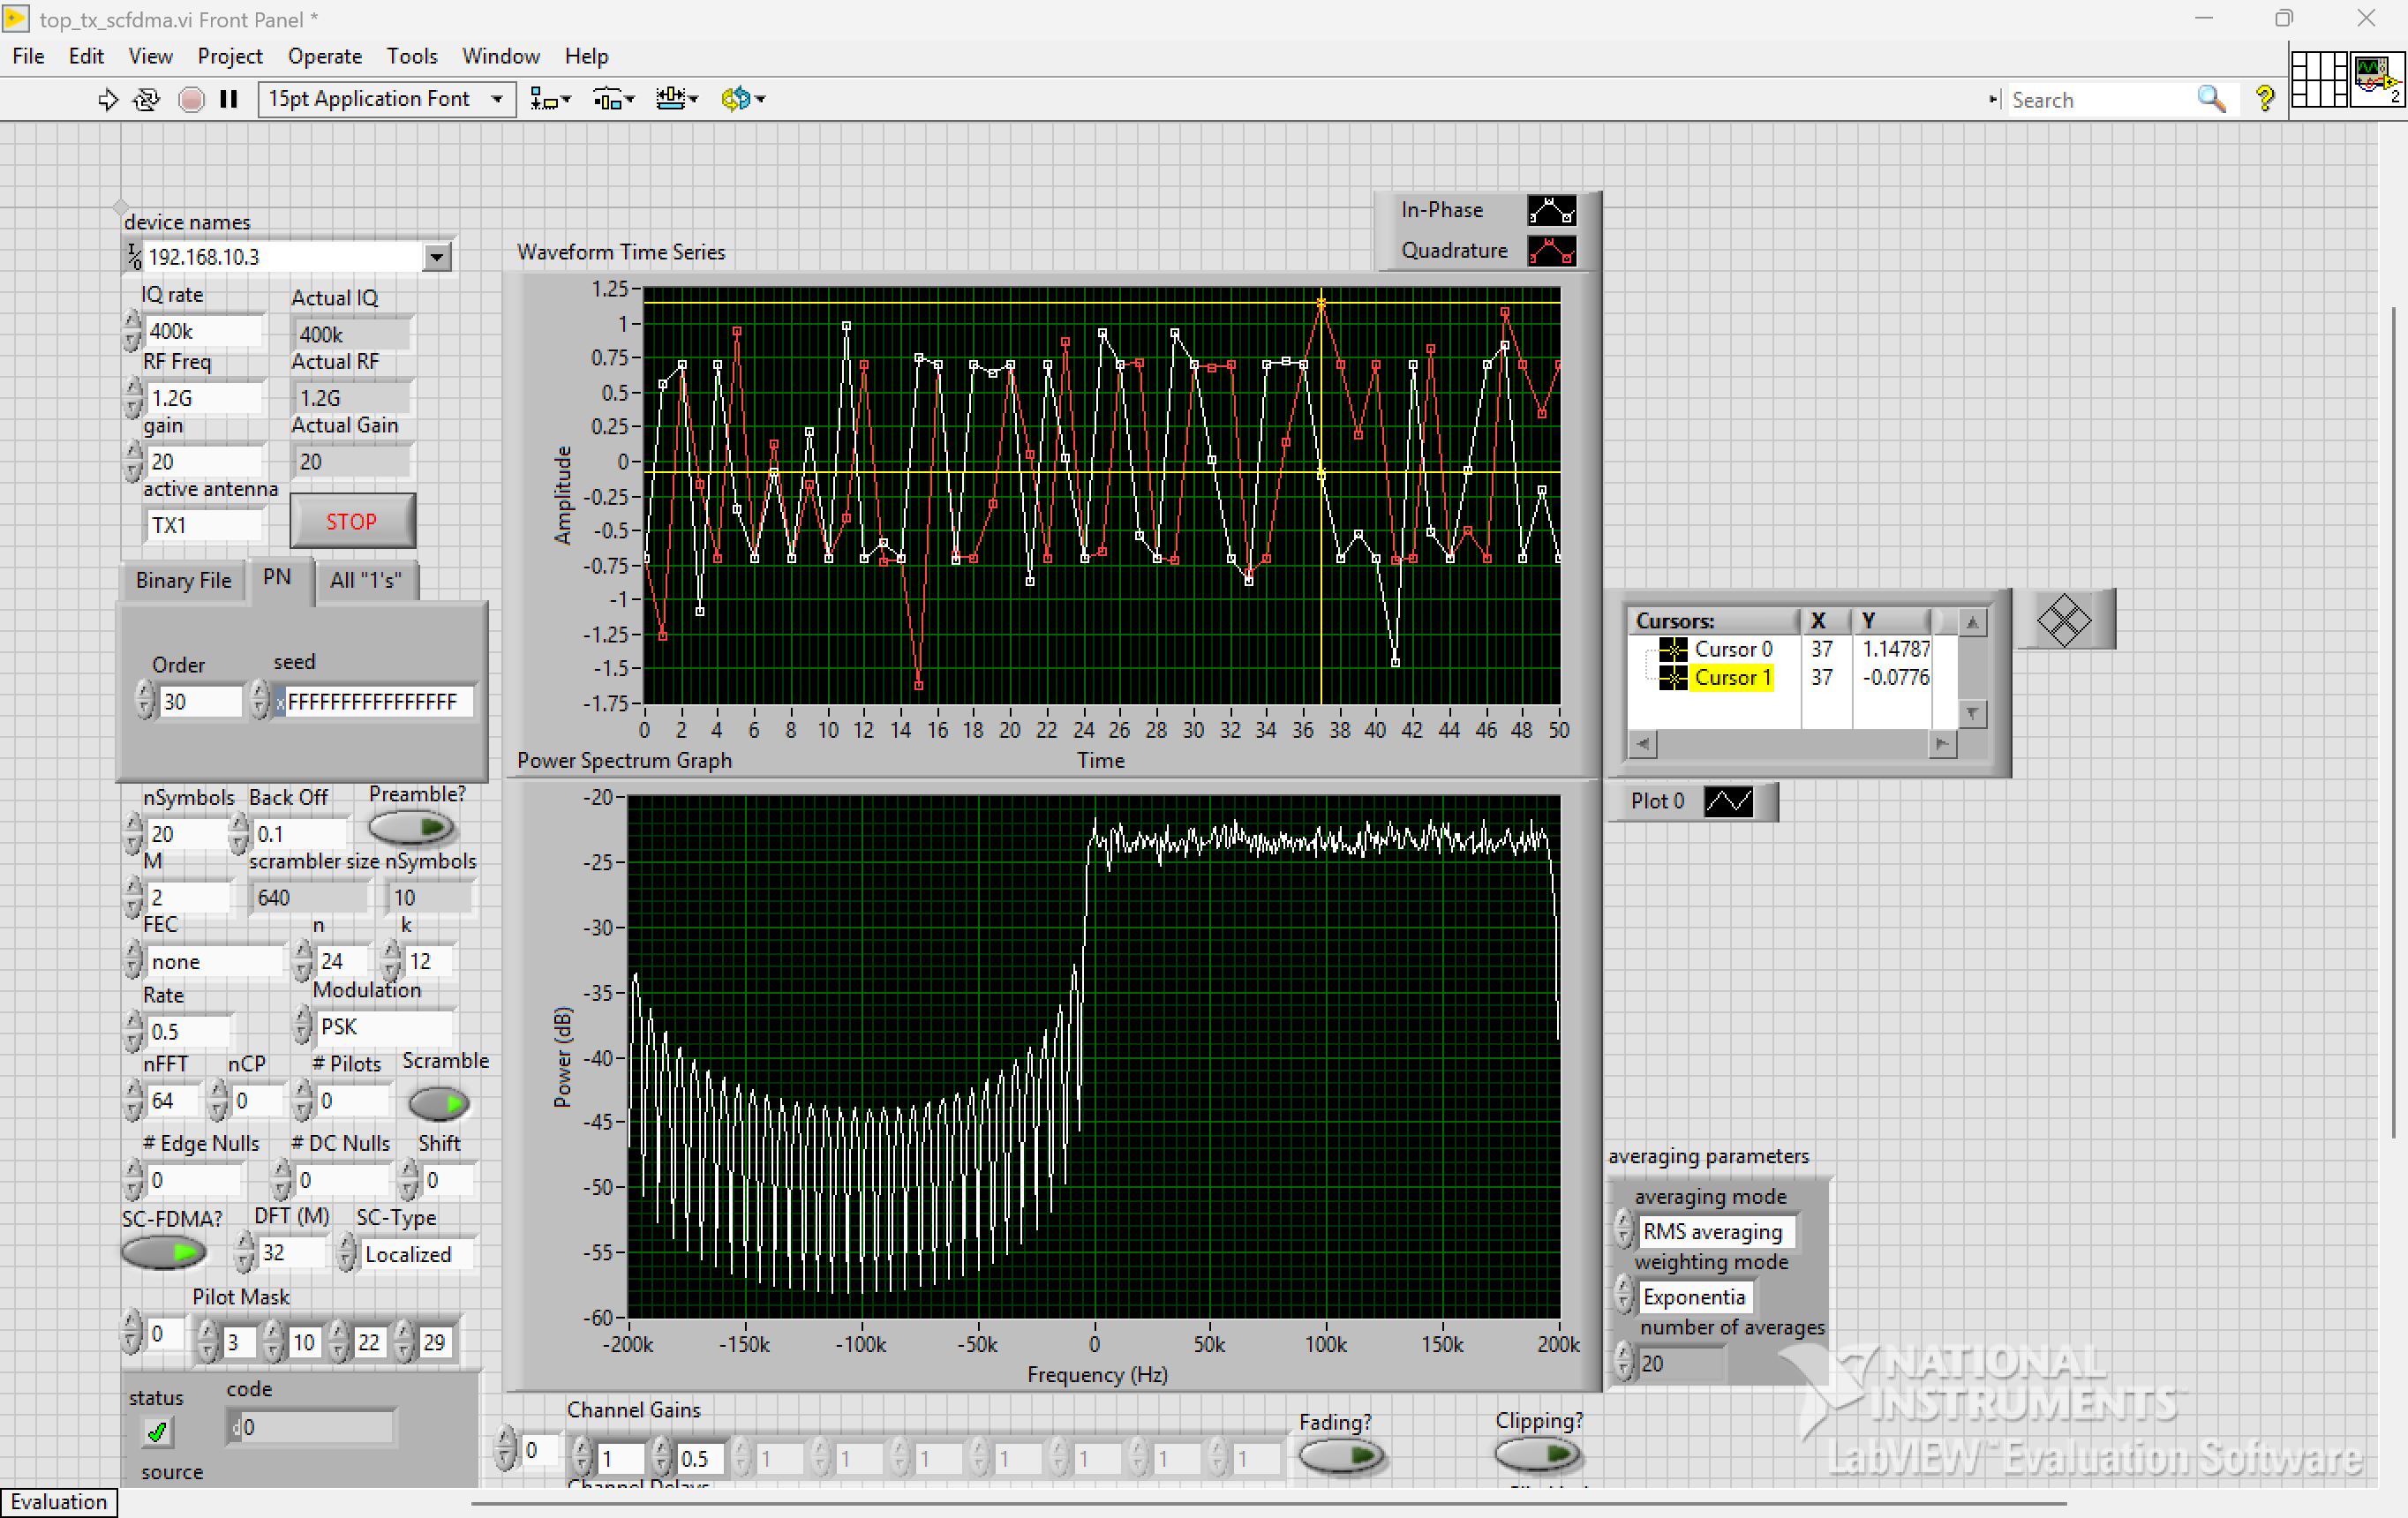
\includegraphics[width=0.7\textwidth]{lab_ss/WES268B_Lab7_Part2-2-6_Tx_Localized_DFT-32_PAPR-1.22dB_idk.png}
    \caption{Lab 7 - SC-FDMA, SC-Type Localized, DFT Size = 32, PAPR = 1.22dB}
    %\label{f42}
\end{figure}

% 2.2.7
\subsubsection{ }

\noindent\textbf{Question.}
{
    What type of modulation format does the time-series look like? Can you notice a pattern in the time-series 
    for each value of DFT (M)?
}
\noindent\textbf{Answer.} 
{
    The localized SC-type waveform has a higher PAPR because the energy is localized to adjacent subcarriers only which leads to greater 
    envelope fluctuation. The interleaved SC-type waveform has a periodic repetition at $\frac{N_{FFT}}{M_{DFT}}$ and as $M_{DFT}$ decreases, 
    the periodicity is more noticeable. The time series looks similar to upsampled single-carrier QPSK.
}

% 3 Peak to Average Power Ratio (PAPR)
\section{Channel Estimation and Impairments}

% 3.1.1
\subsubsection{ }

% 3.1.2
\subsection{Pilot-Based Phase Estimation}
\begin{figure}[H]
    \centering
    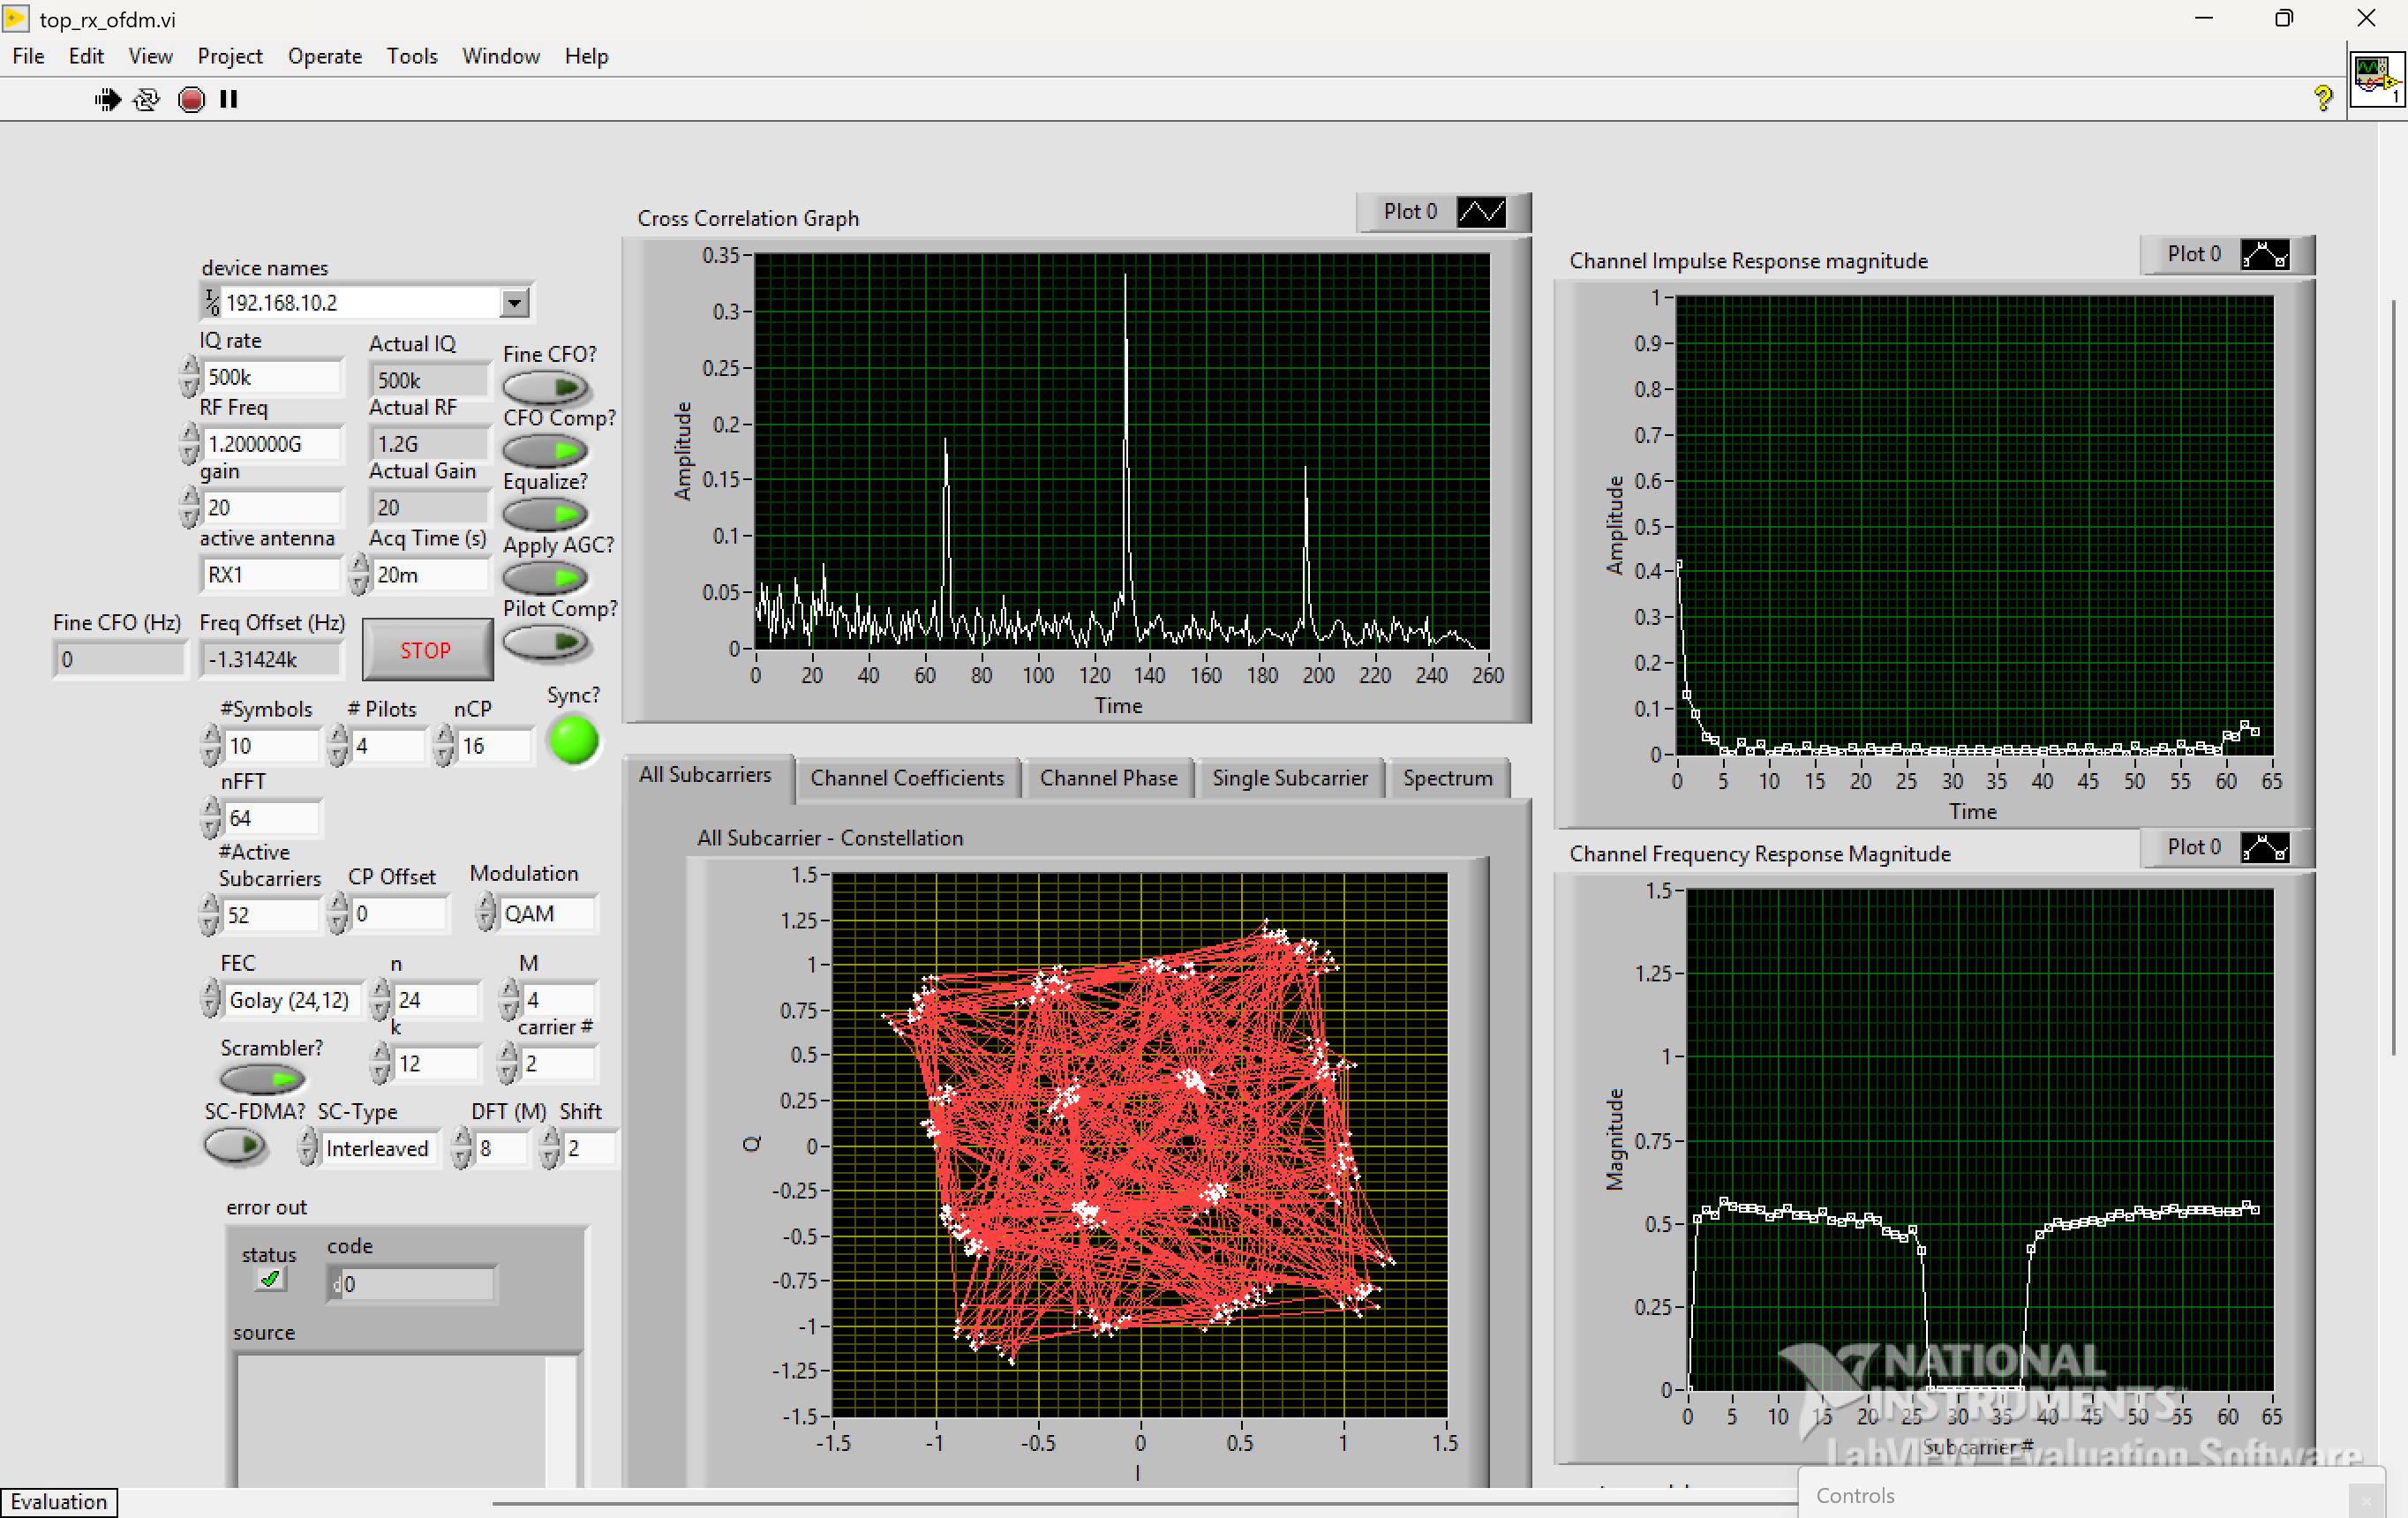
\includegraphics[width=0.7\textwidth]{lab_ss/WES268B_Lab7_Part3-1-2_Rx_PilotComp-OFF.png}
    \caption{Lab 7 - INSERT}
    %\label{f43}
\end{figure}

\begin{figure}[H]
    \centering
    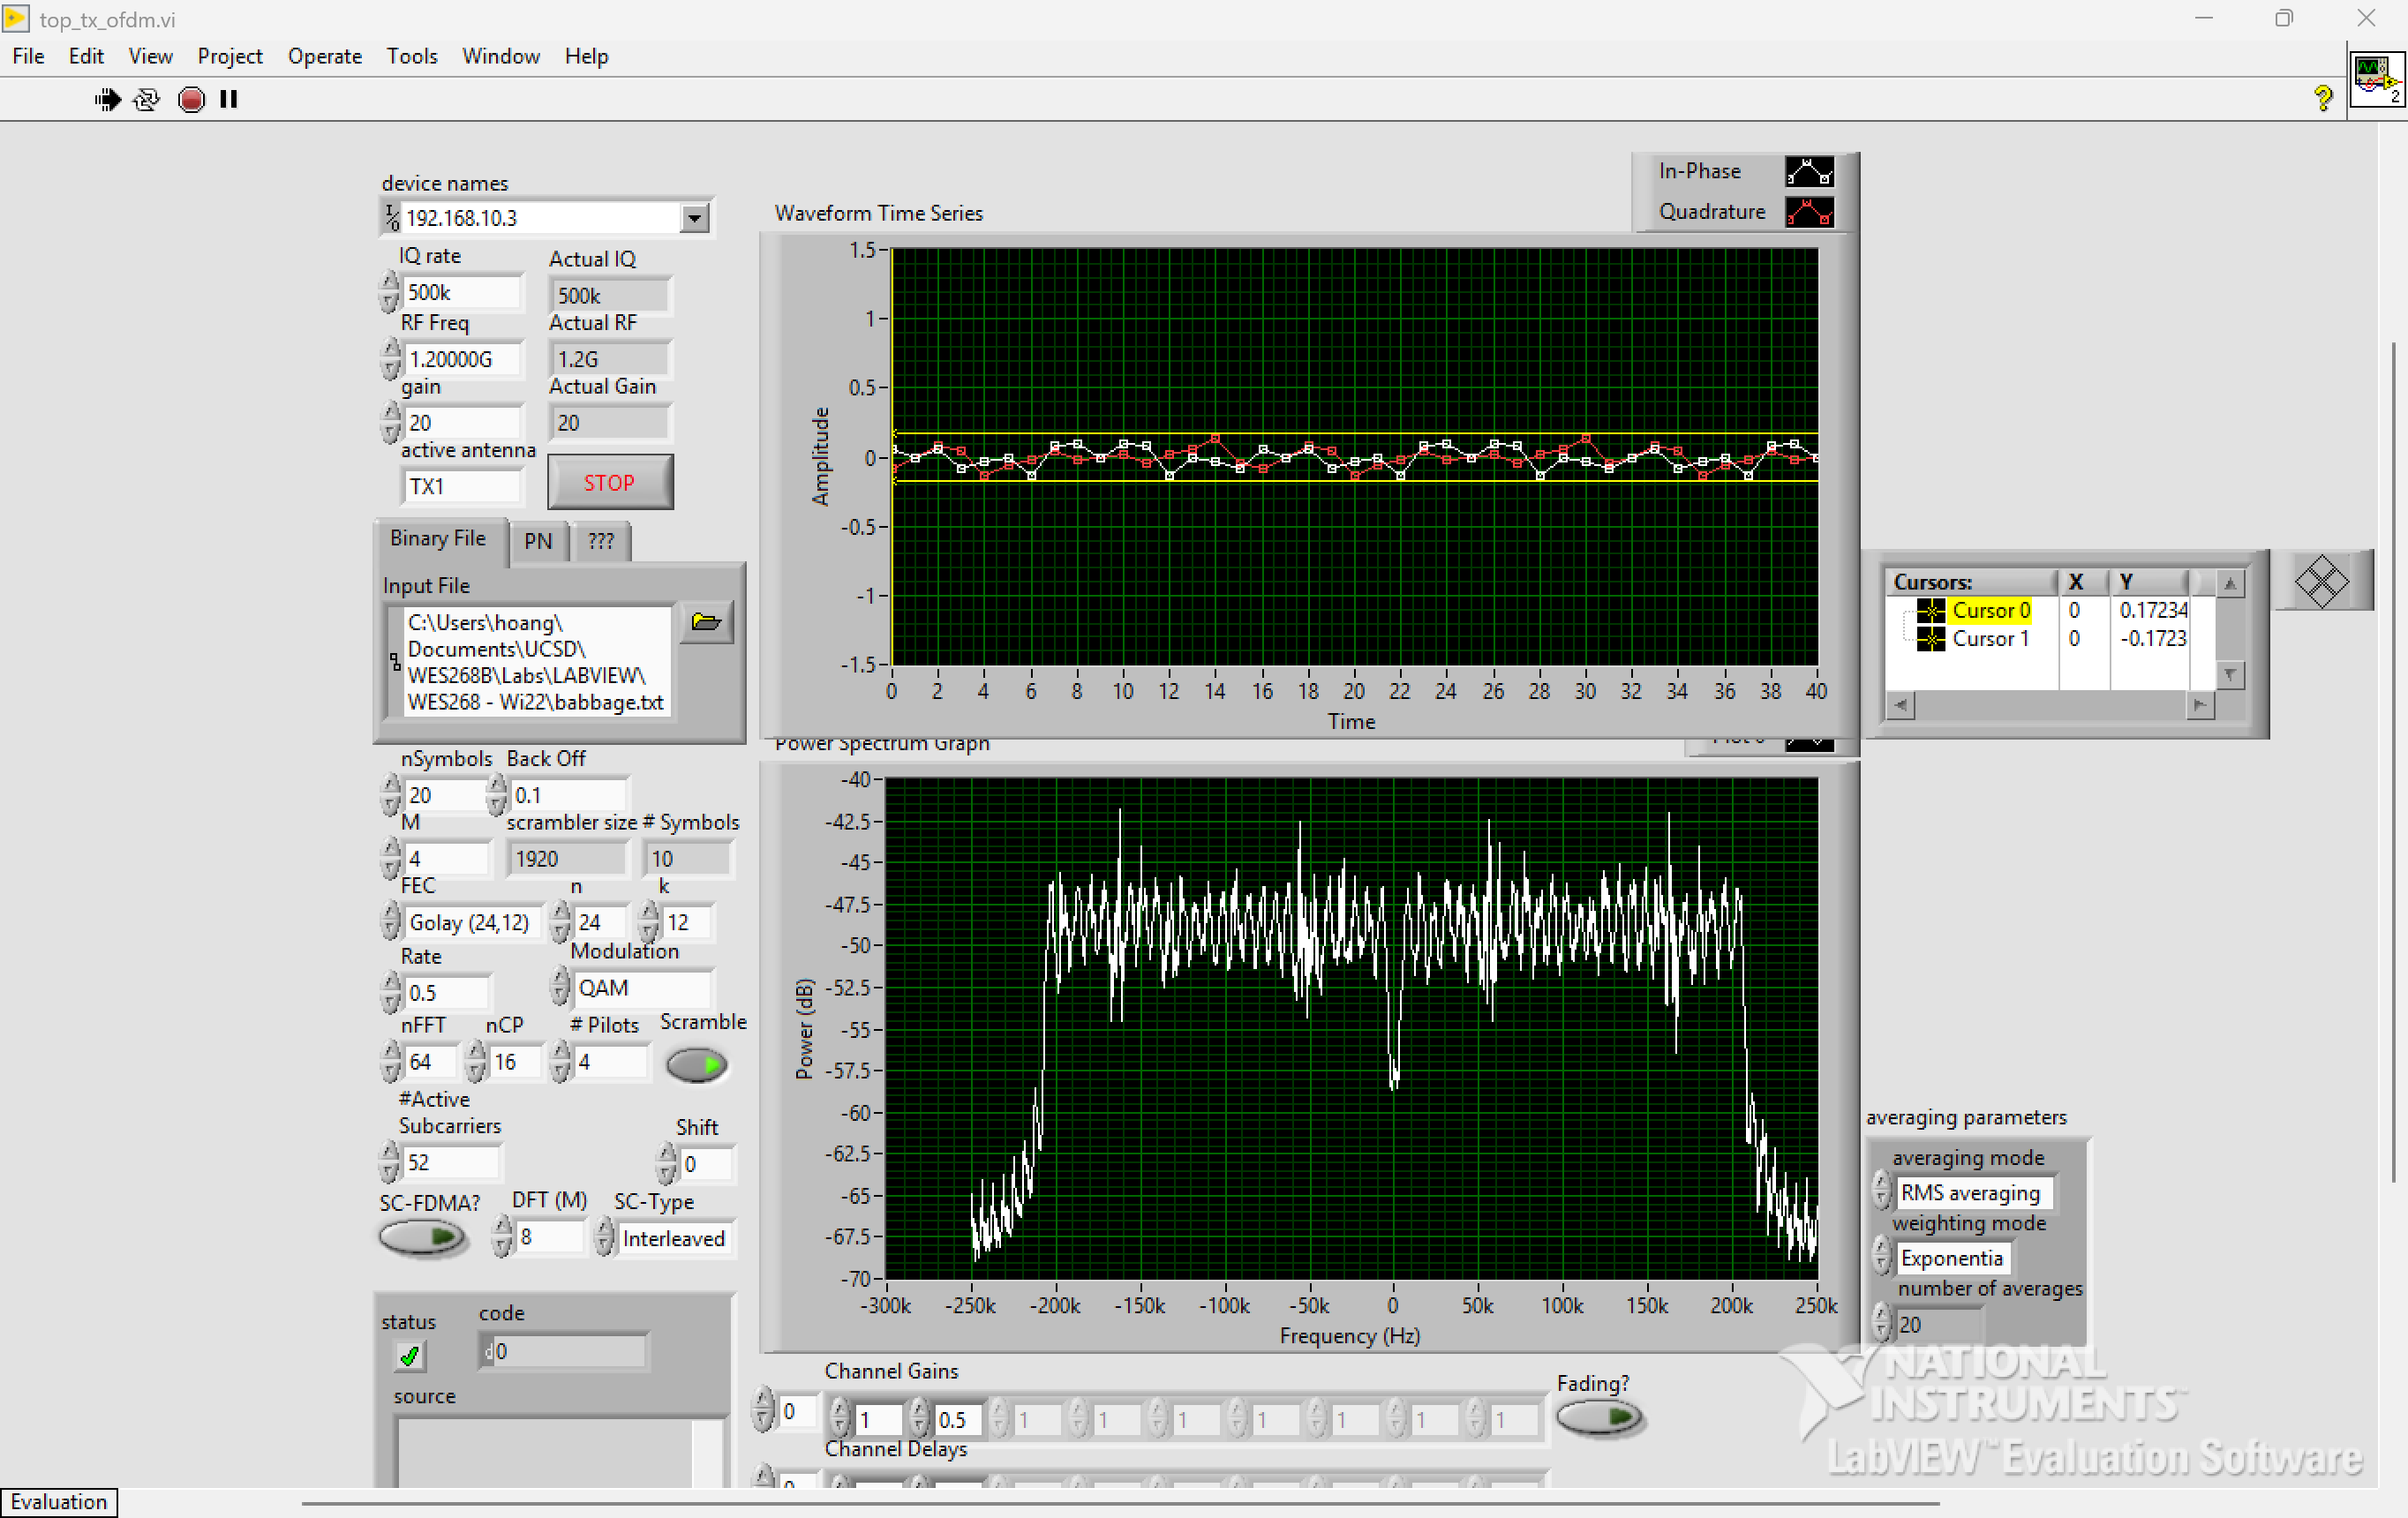
\includegraphics[width=0.7\textwidth]{lab_ss/WES268B_Lab7_Part3-1-2_Tx.png}
    \caption{Lab 7 - INSERT}
    %\label{f44}
\end{figure}

% 3.1.3
\subsection{}
\begin{figure}[H]
    \centering
    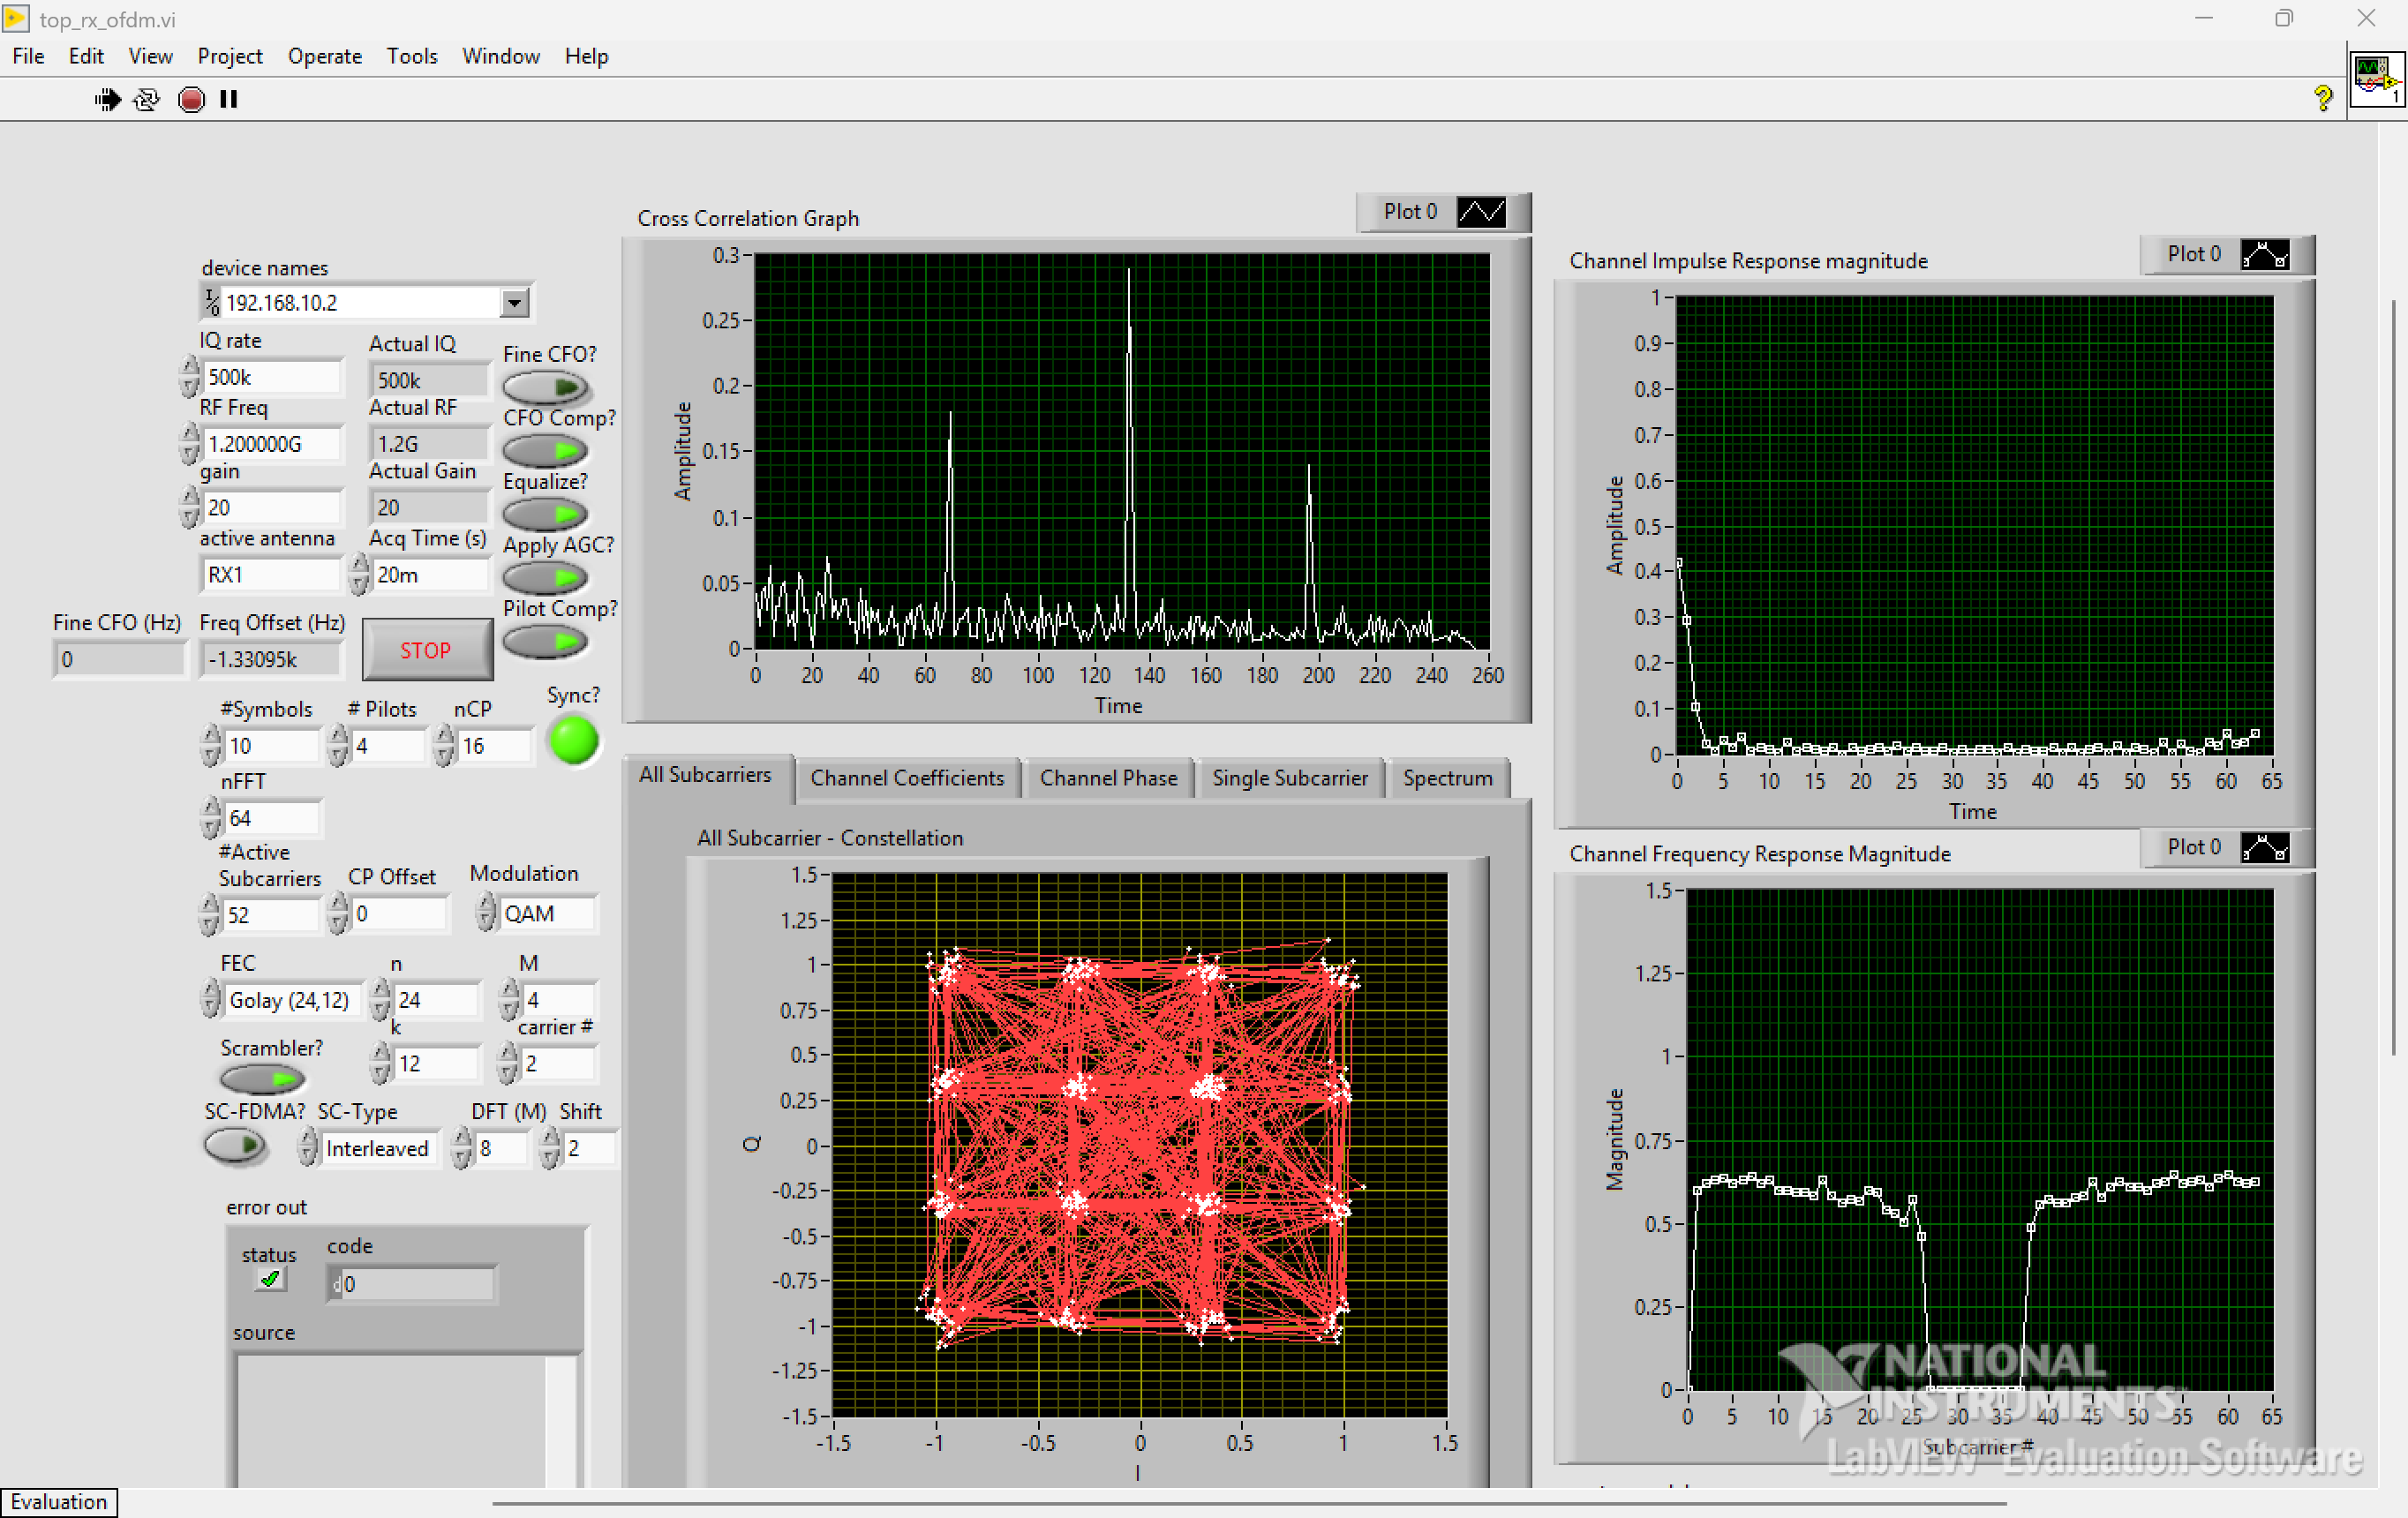
\includegraphics[width=0.7\textwidth]{lab_ss/WES268B_Lab7_Part3-1-3_Rx_PilotComp-ON.png}
    \caption{Lab 7 - INSERT}
    %\label{f45}
\end{figure}

% 3.1.4
\subsection{}
\begin{figure}[H]
    \centering
    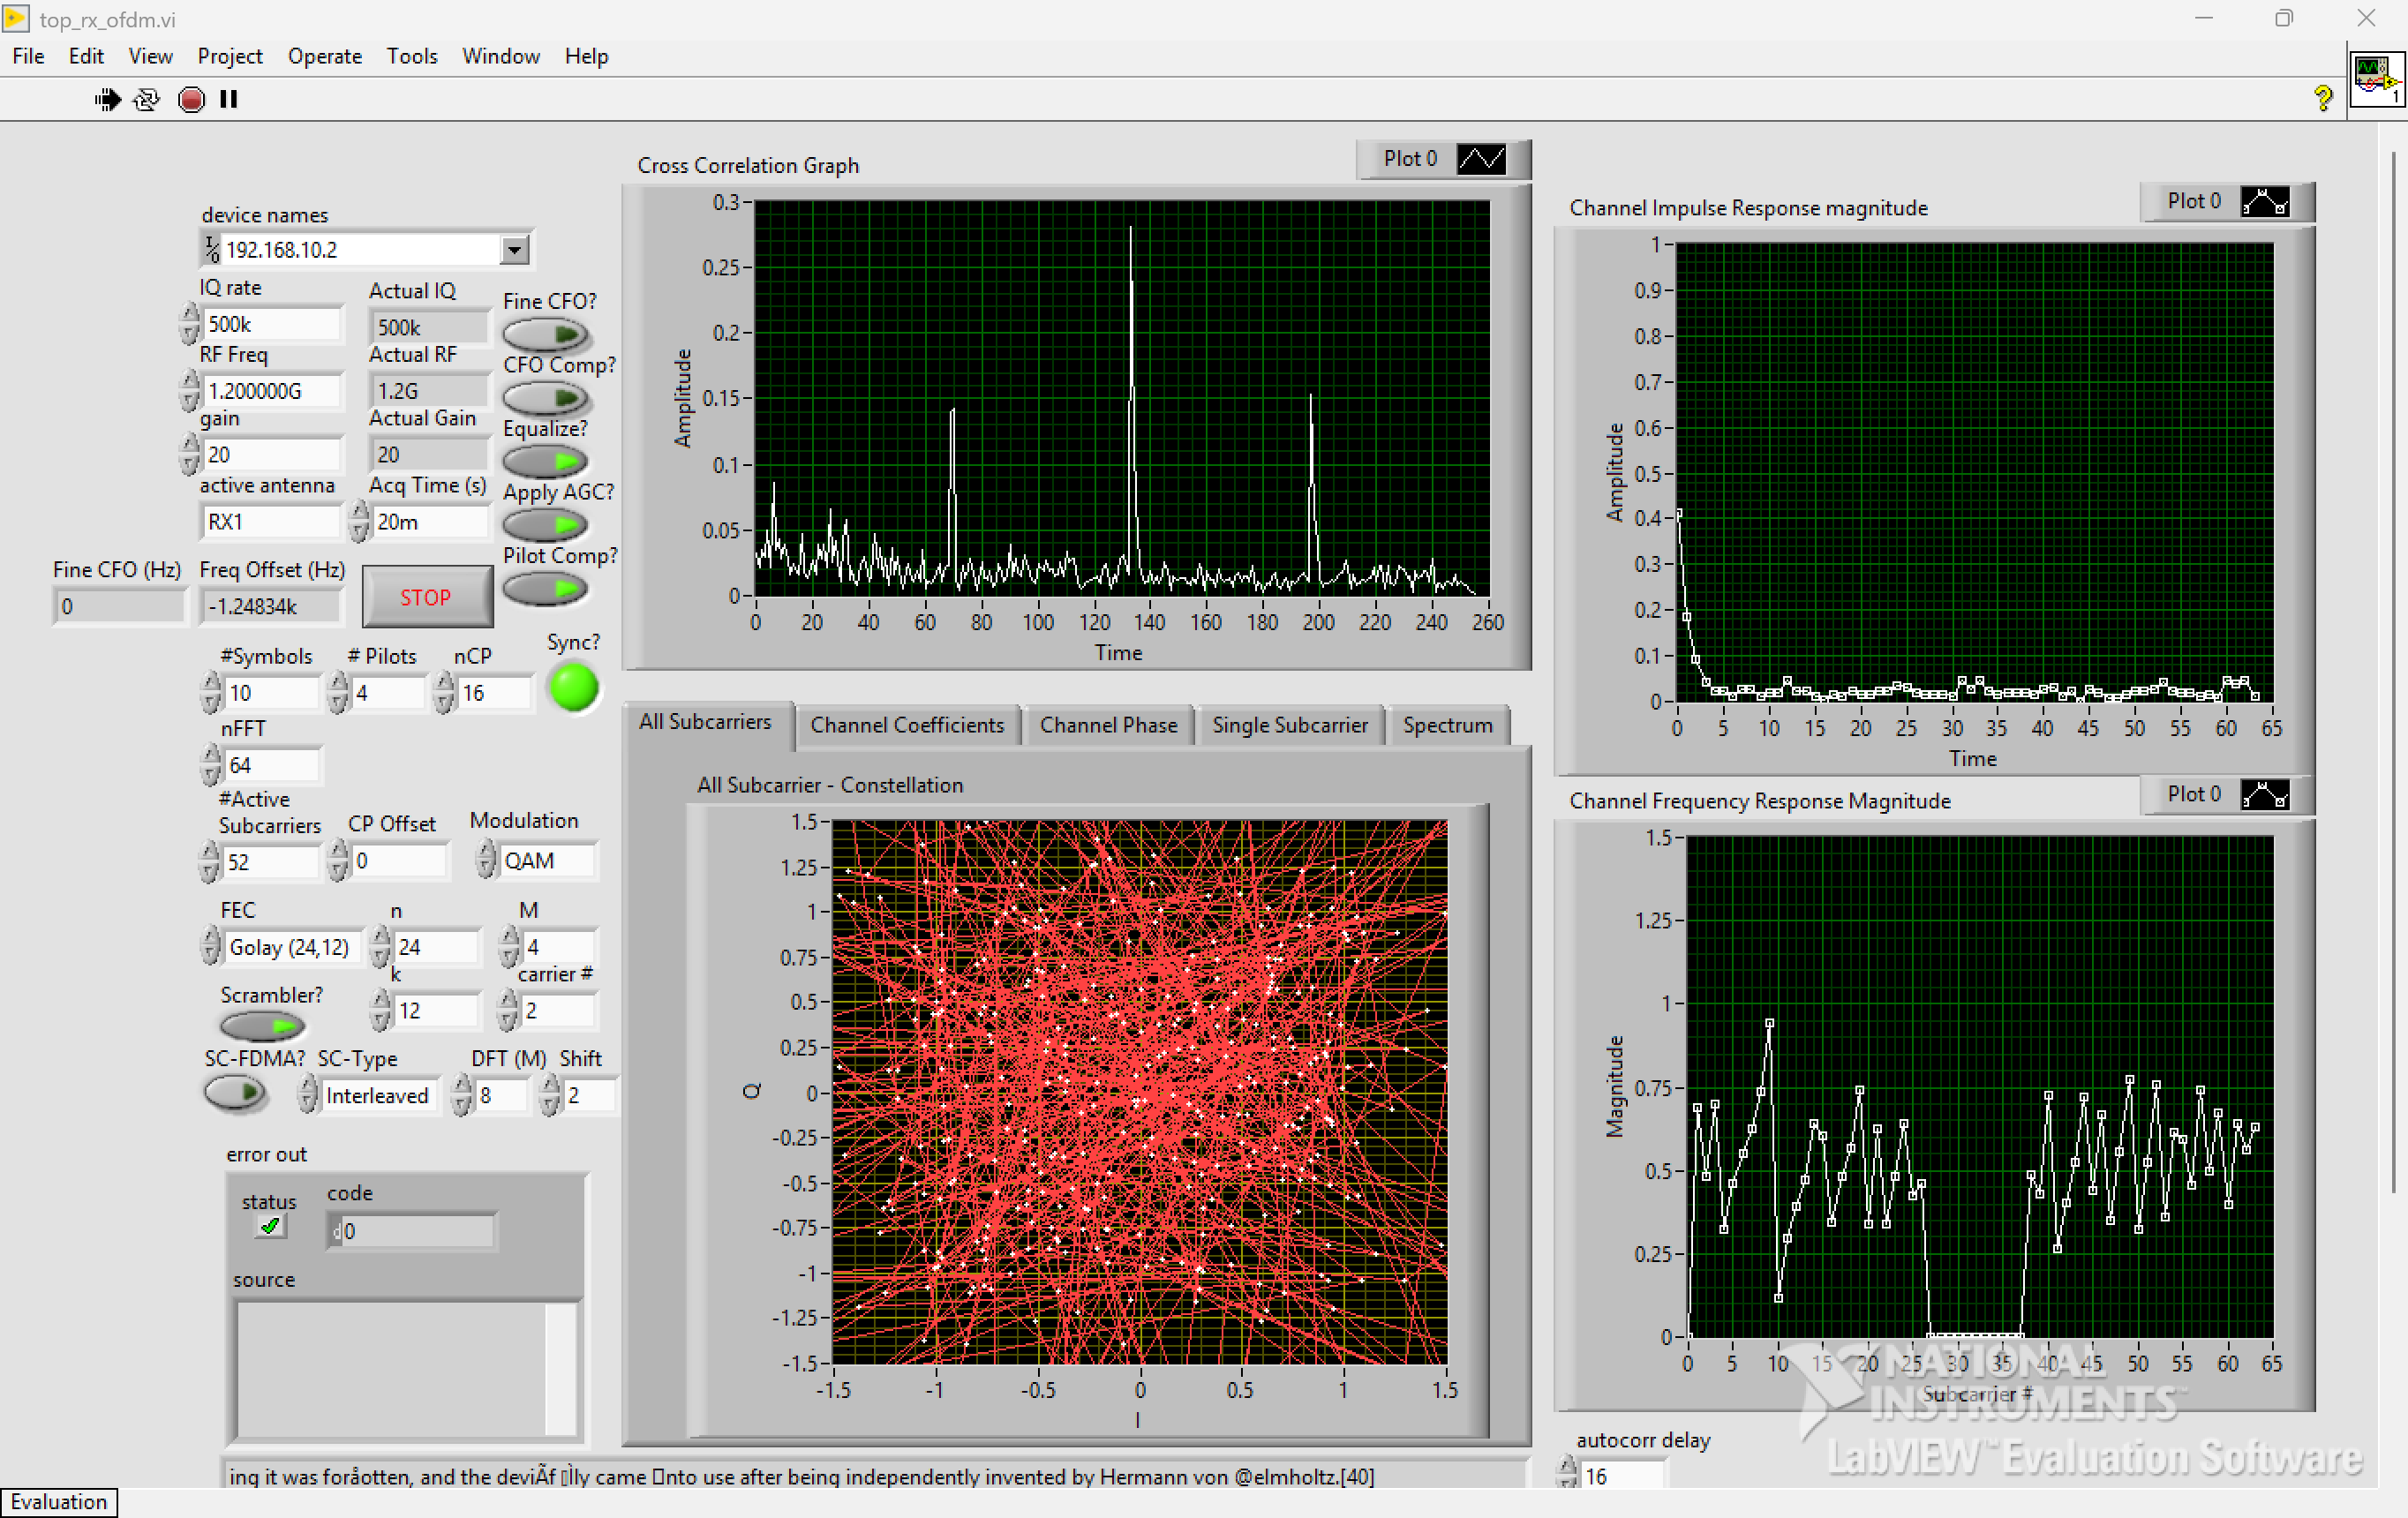
\includegraphics[width=0.7\textwidth]{lab_ss/WES268B_Lab7_Part3-1-4_Rx_PilotComp-ON_FreqComp-OFF.png}
    \caption{Lab 7 - INSERT}
    %\label{f46}
\end{figure}

% 3.1.5
\subsection{}
\begin{figure}[H]
    \centering
    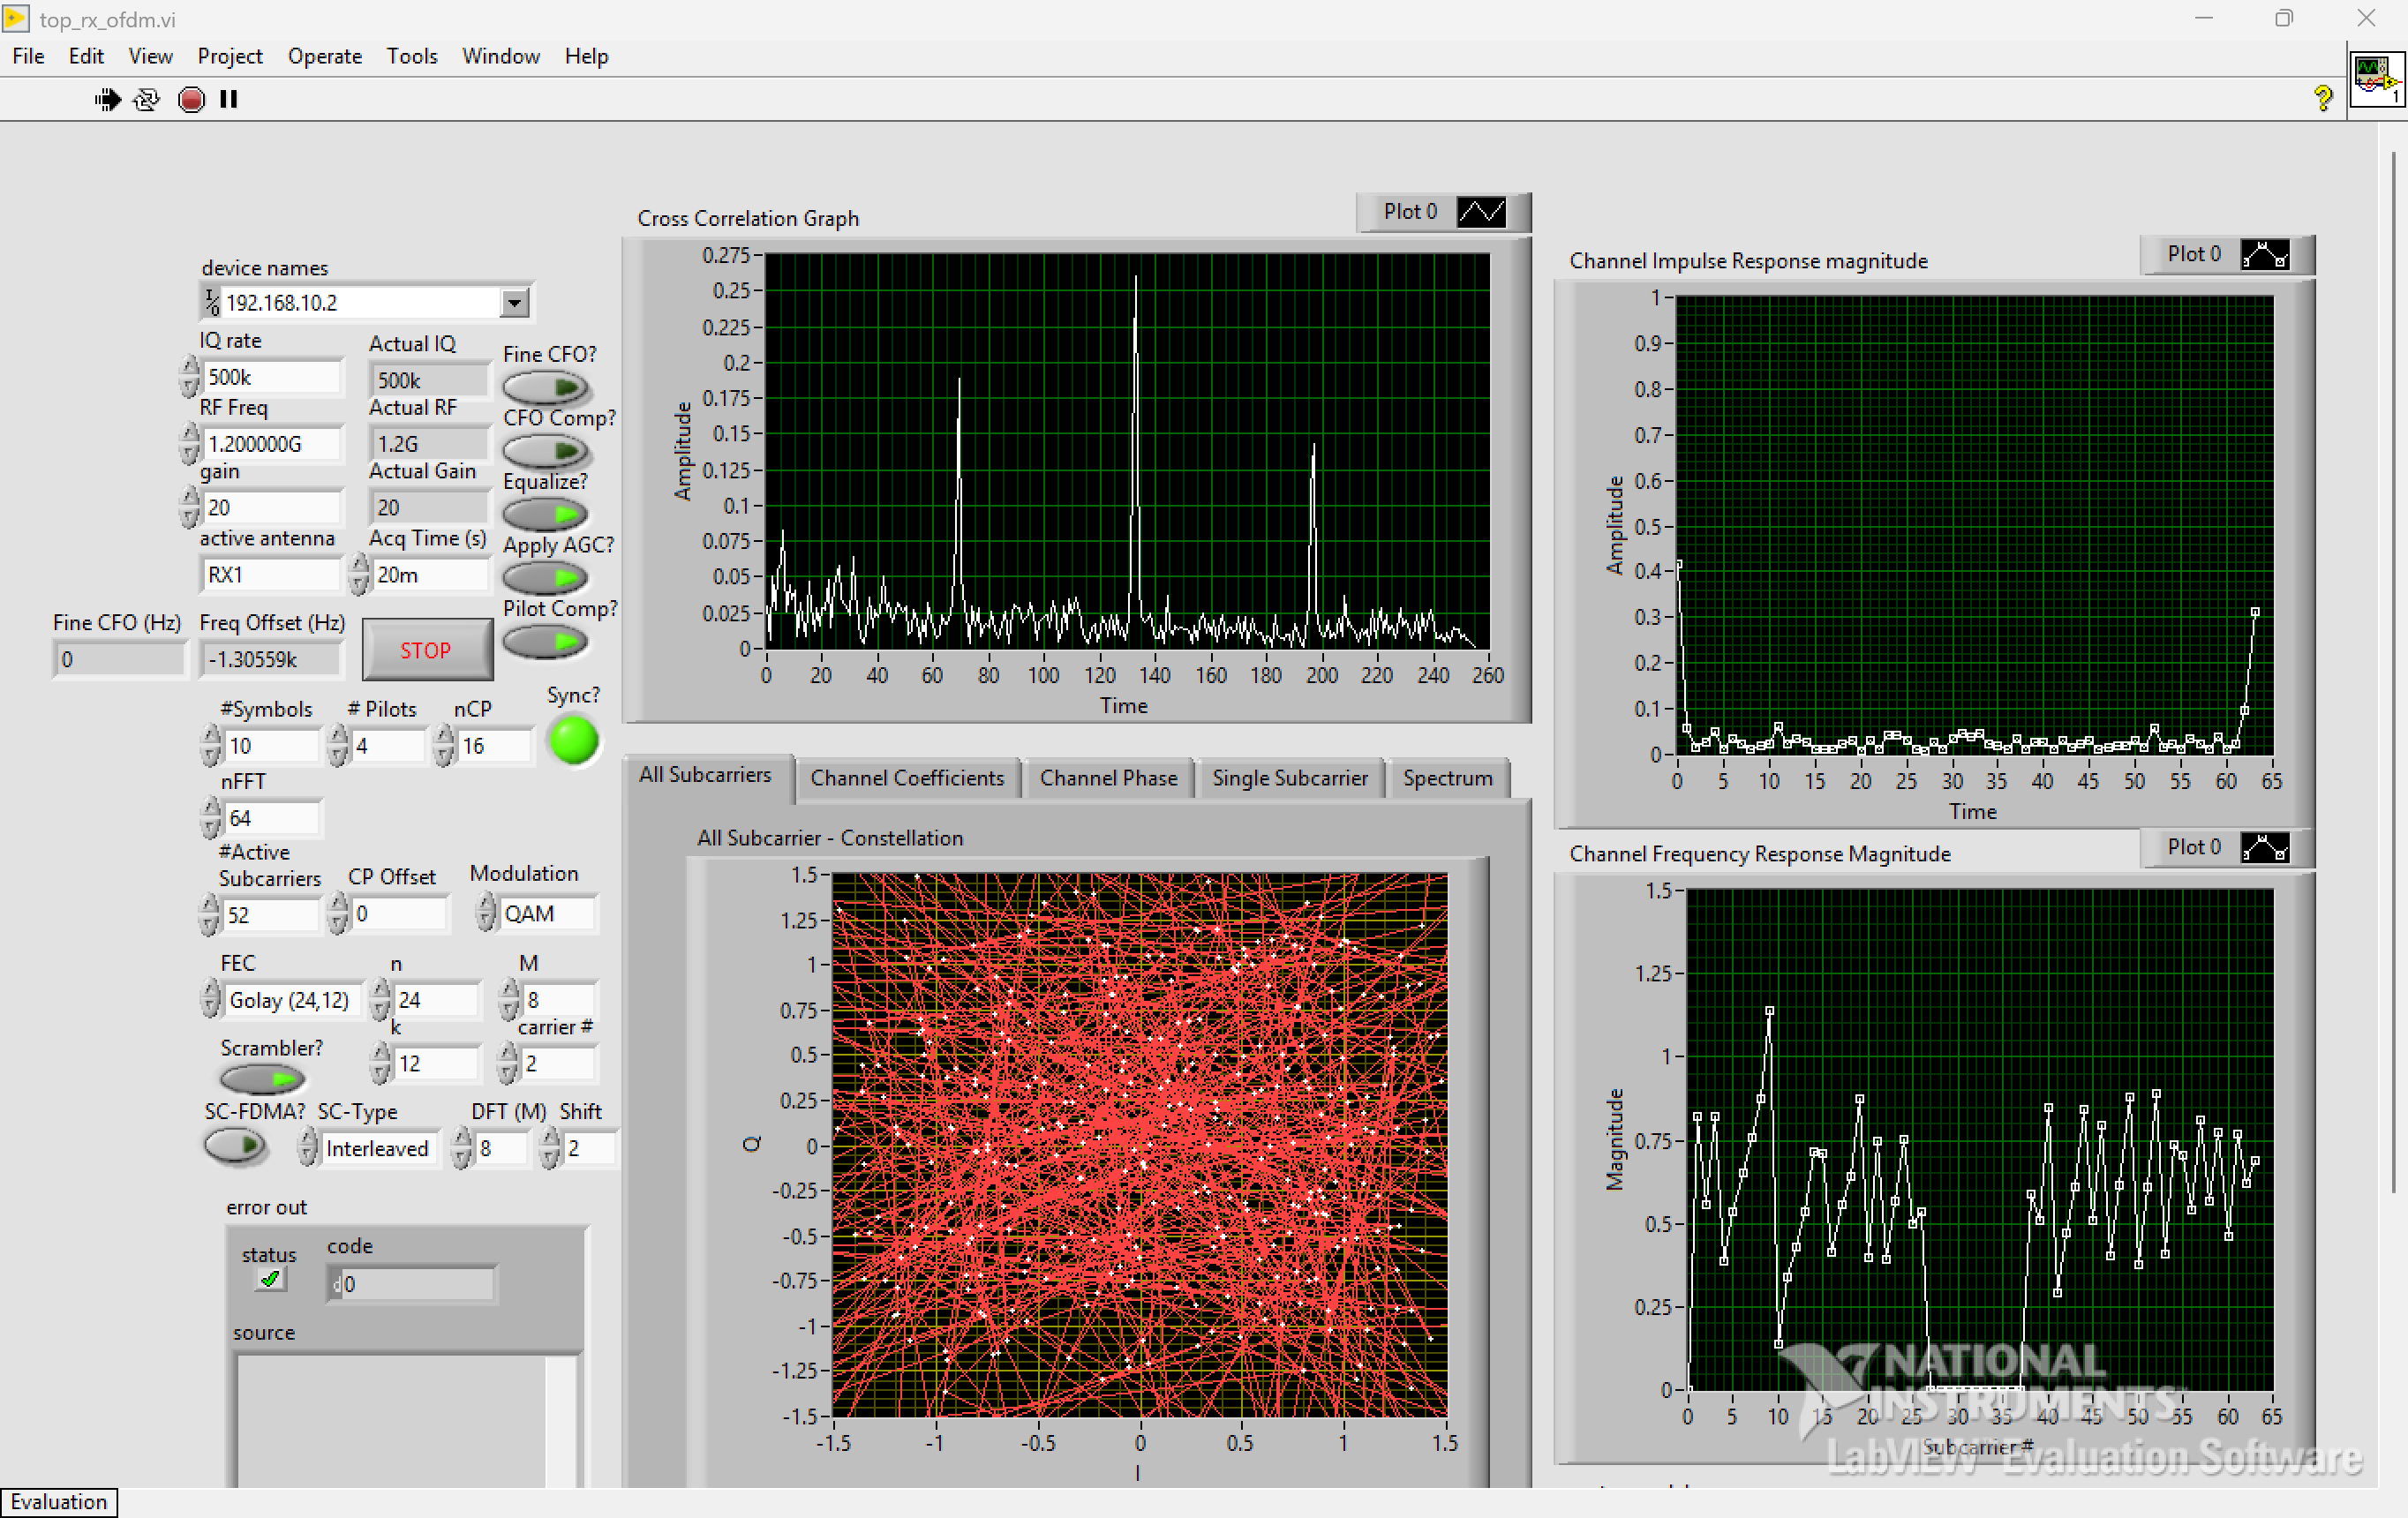
\includegraphics[width=0.7\textwidth]{lab_ss/WES268B_Lab7_Part3-1-5_Rx-64QAM_PilotComp-ON_FreqComp-OFF.png}
    \caption{Lab 7 - INSERT}
    %\label{f47}
\end{figure}

% 3.1.X
\subsubsection{ }

\noindent\textbf{Question.} 

\noindent\textbf{Answer.} 

% 3.2
\subsection{Carrier Frequency Offset Estimation}

% 3.2.1
\subsubsection{ }
\begin{figure}[H]
    \centering
    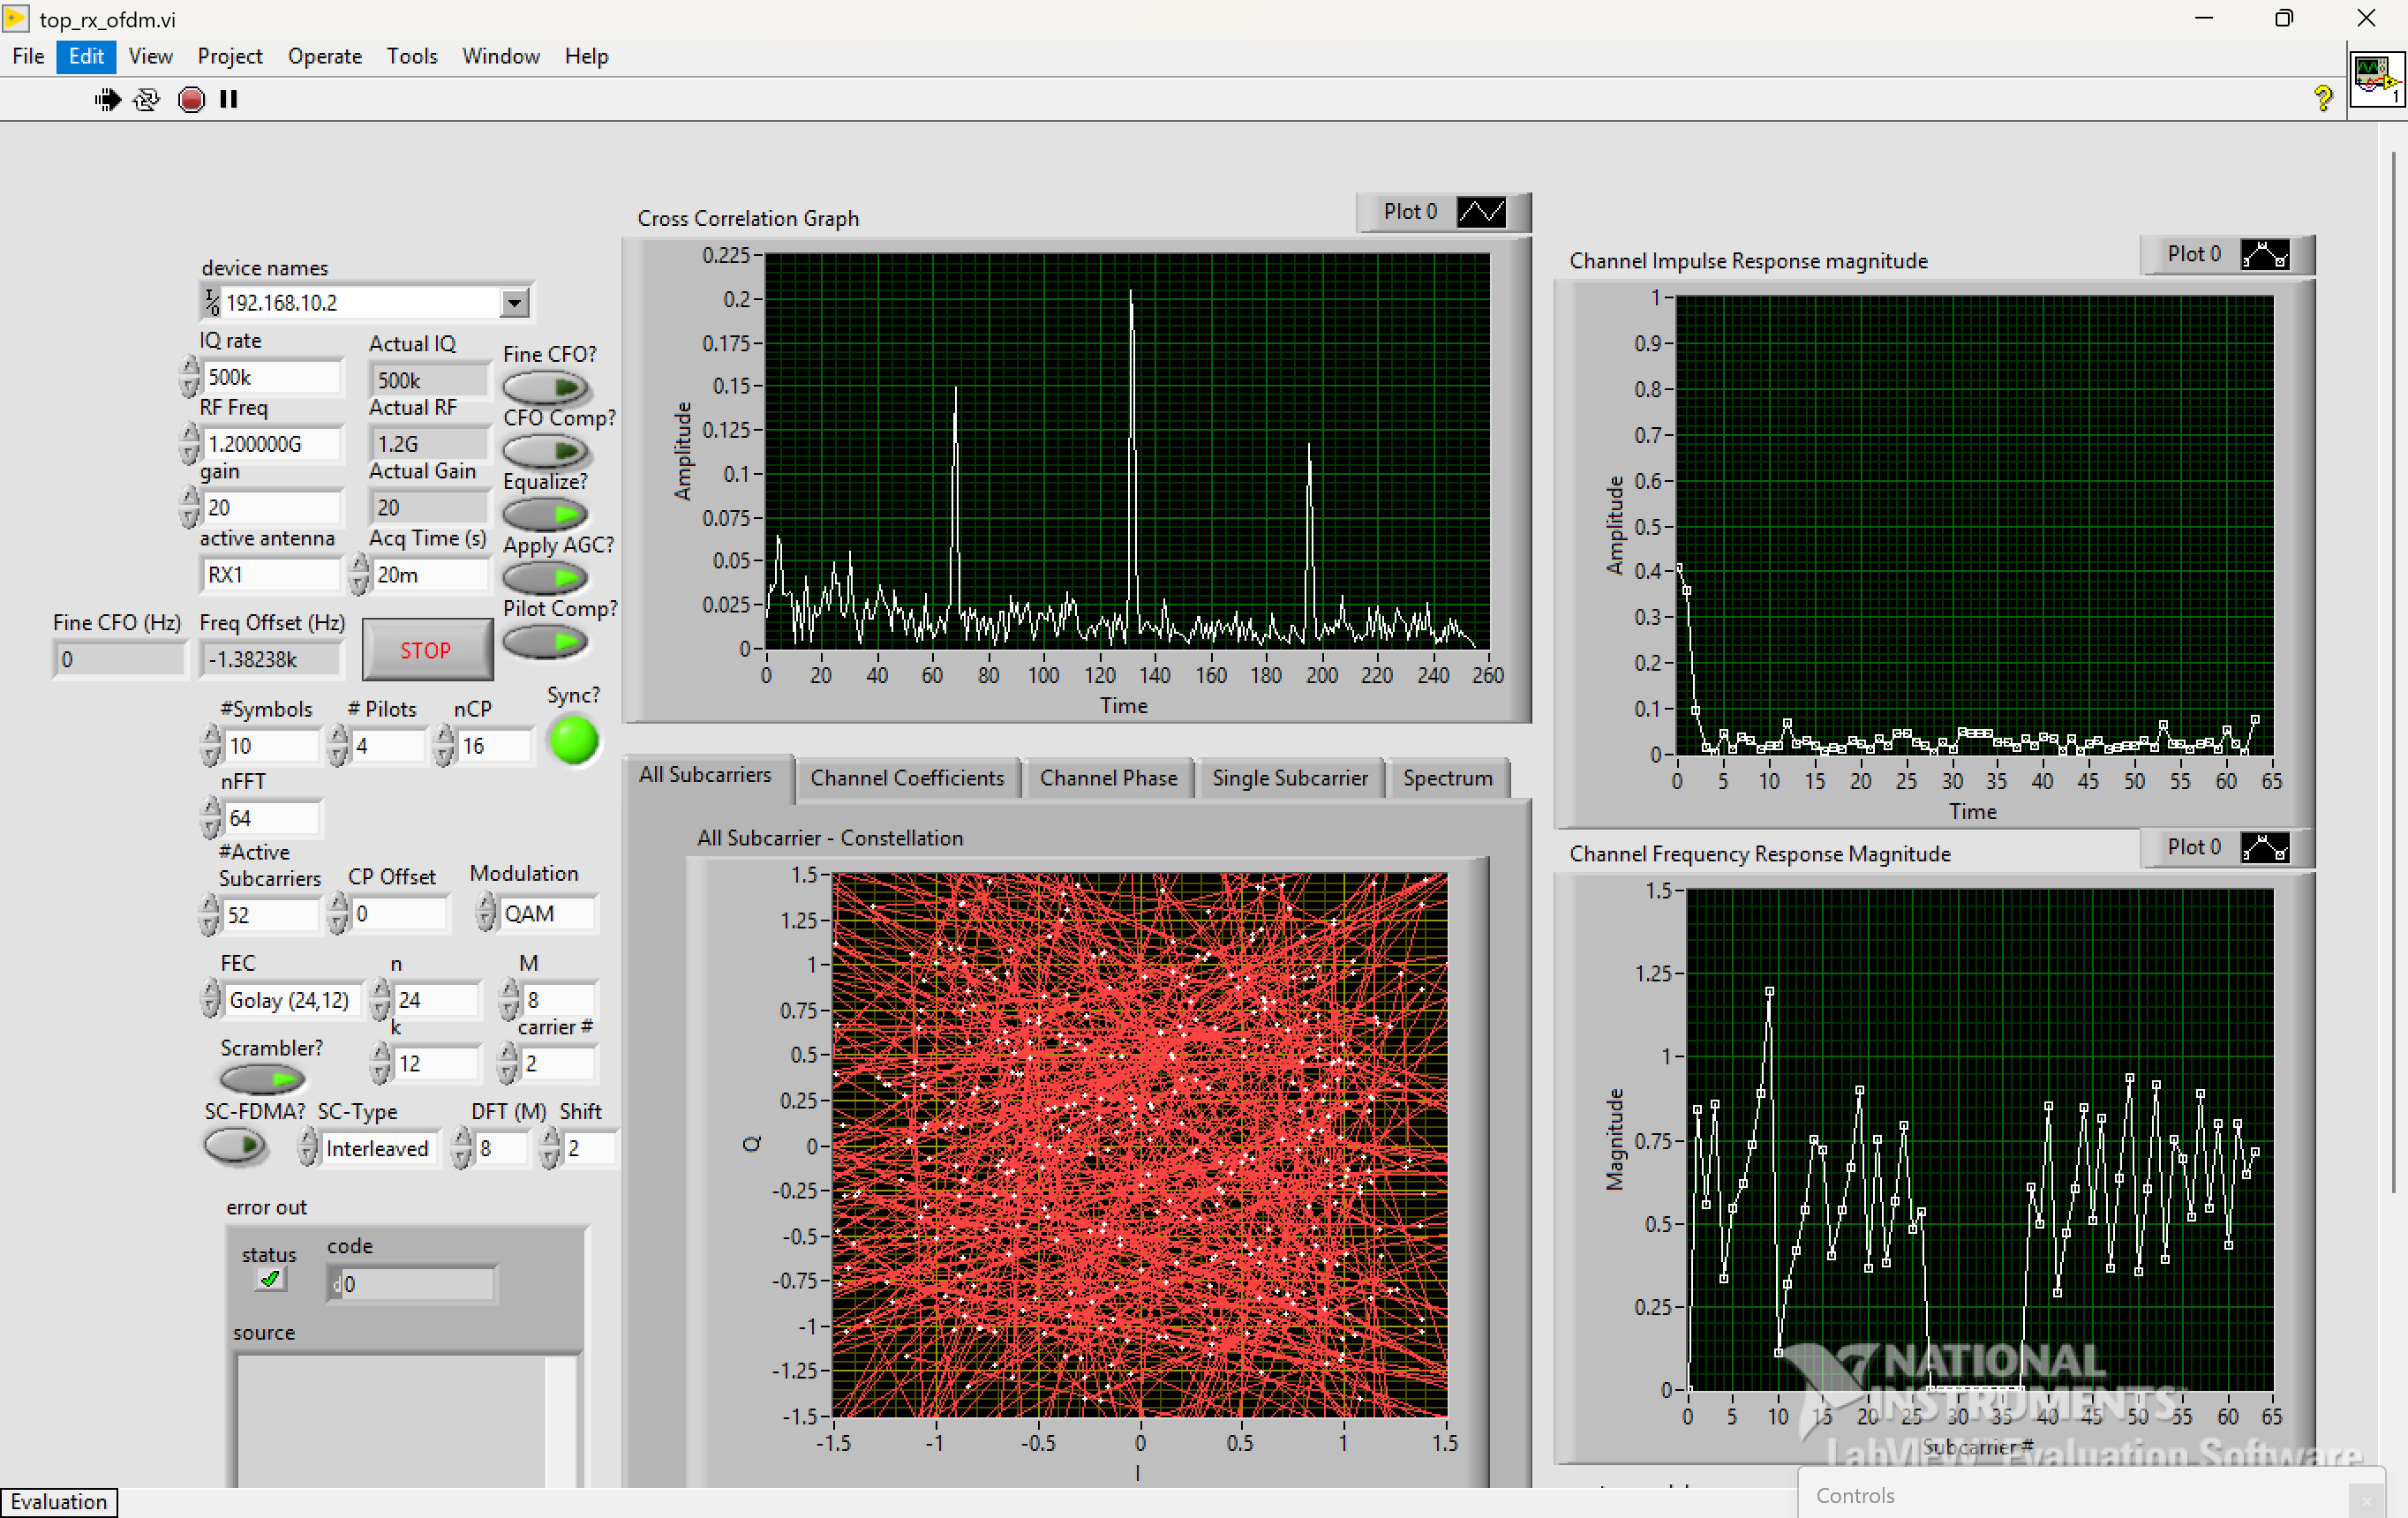
\includegraphics[width=0.7\textwidth]{lab_ss/WES268B_Lab7_Part3-2-1_Rx-64QAM_PilotComp-ON_FreqComp-OFF_FreqOffset-neg1p38kHz.png}
    \caption{Lab 7 - INSERT}
    %\label{f48}
\end{figure}

% 3.2.2
\subsubsection{ }

% 3.2.3
\subsubsection{ }
\begin{figure}[H]
    \centering
    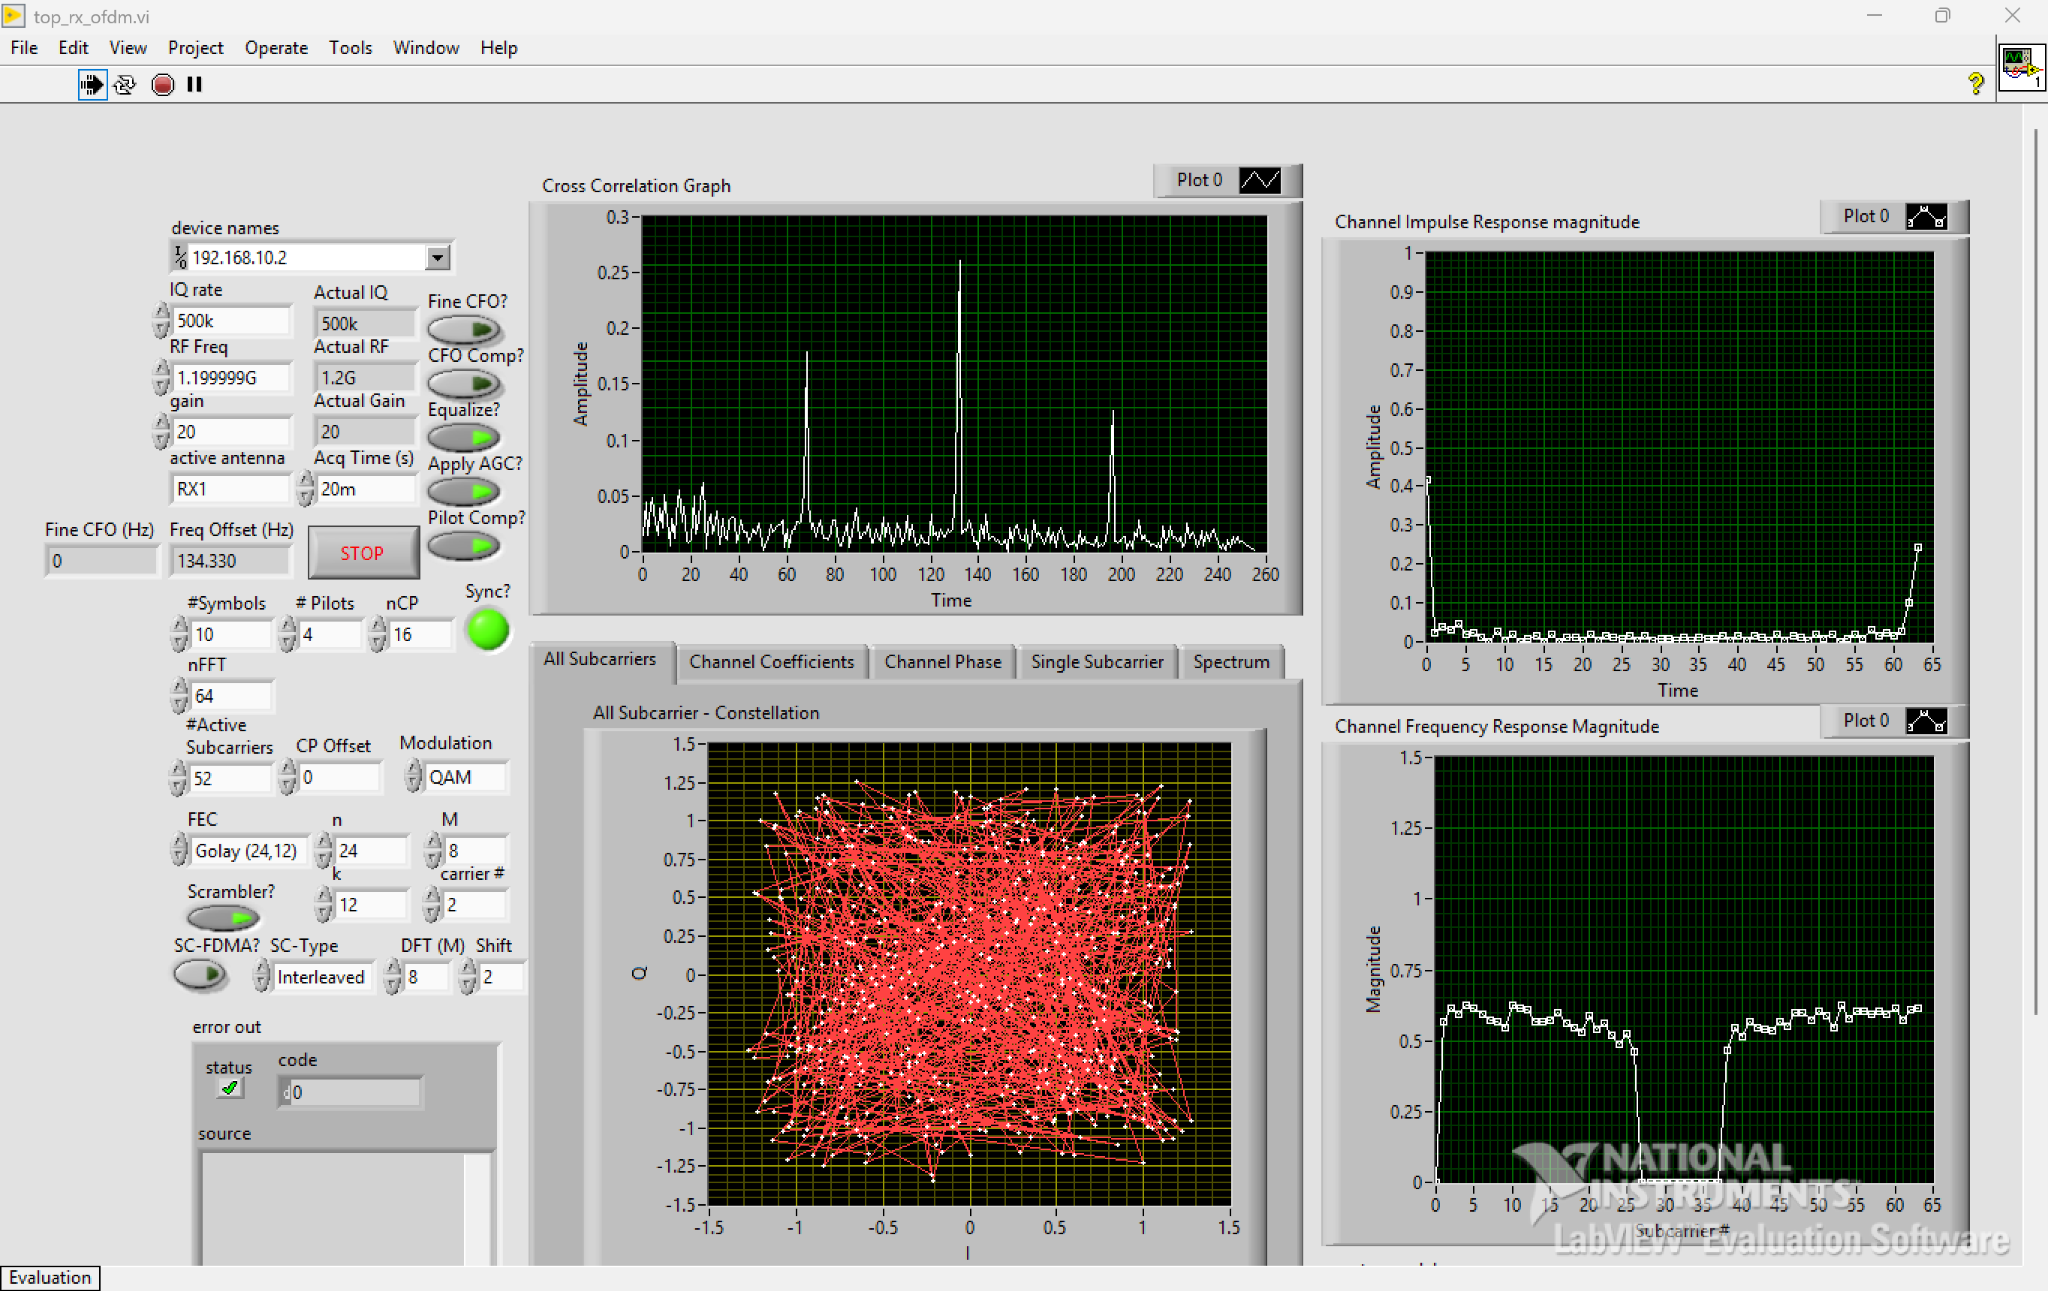
\includegraphics[width=0.7\textwidth]{lab_ss/WES268B_Lab7_Part3-2-3_CorrectedFc.png}
    \caption{Lab 7 - INSERT}
    %\label{f49}
\end{figure}

% 3.2.4
\subsubsection{ }
\begin{figure}[H]
    \centering
    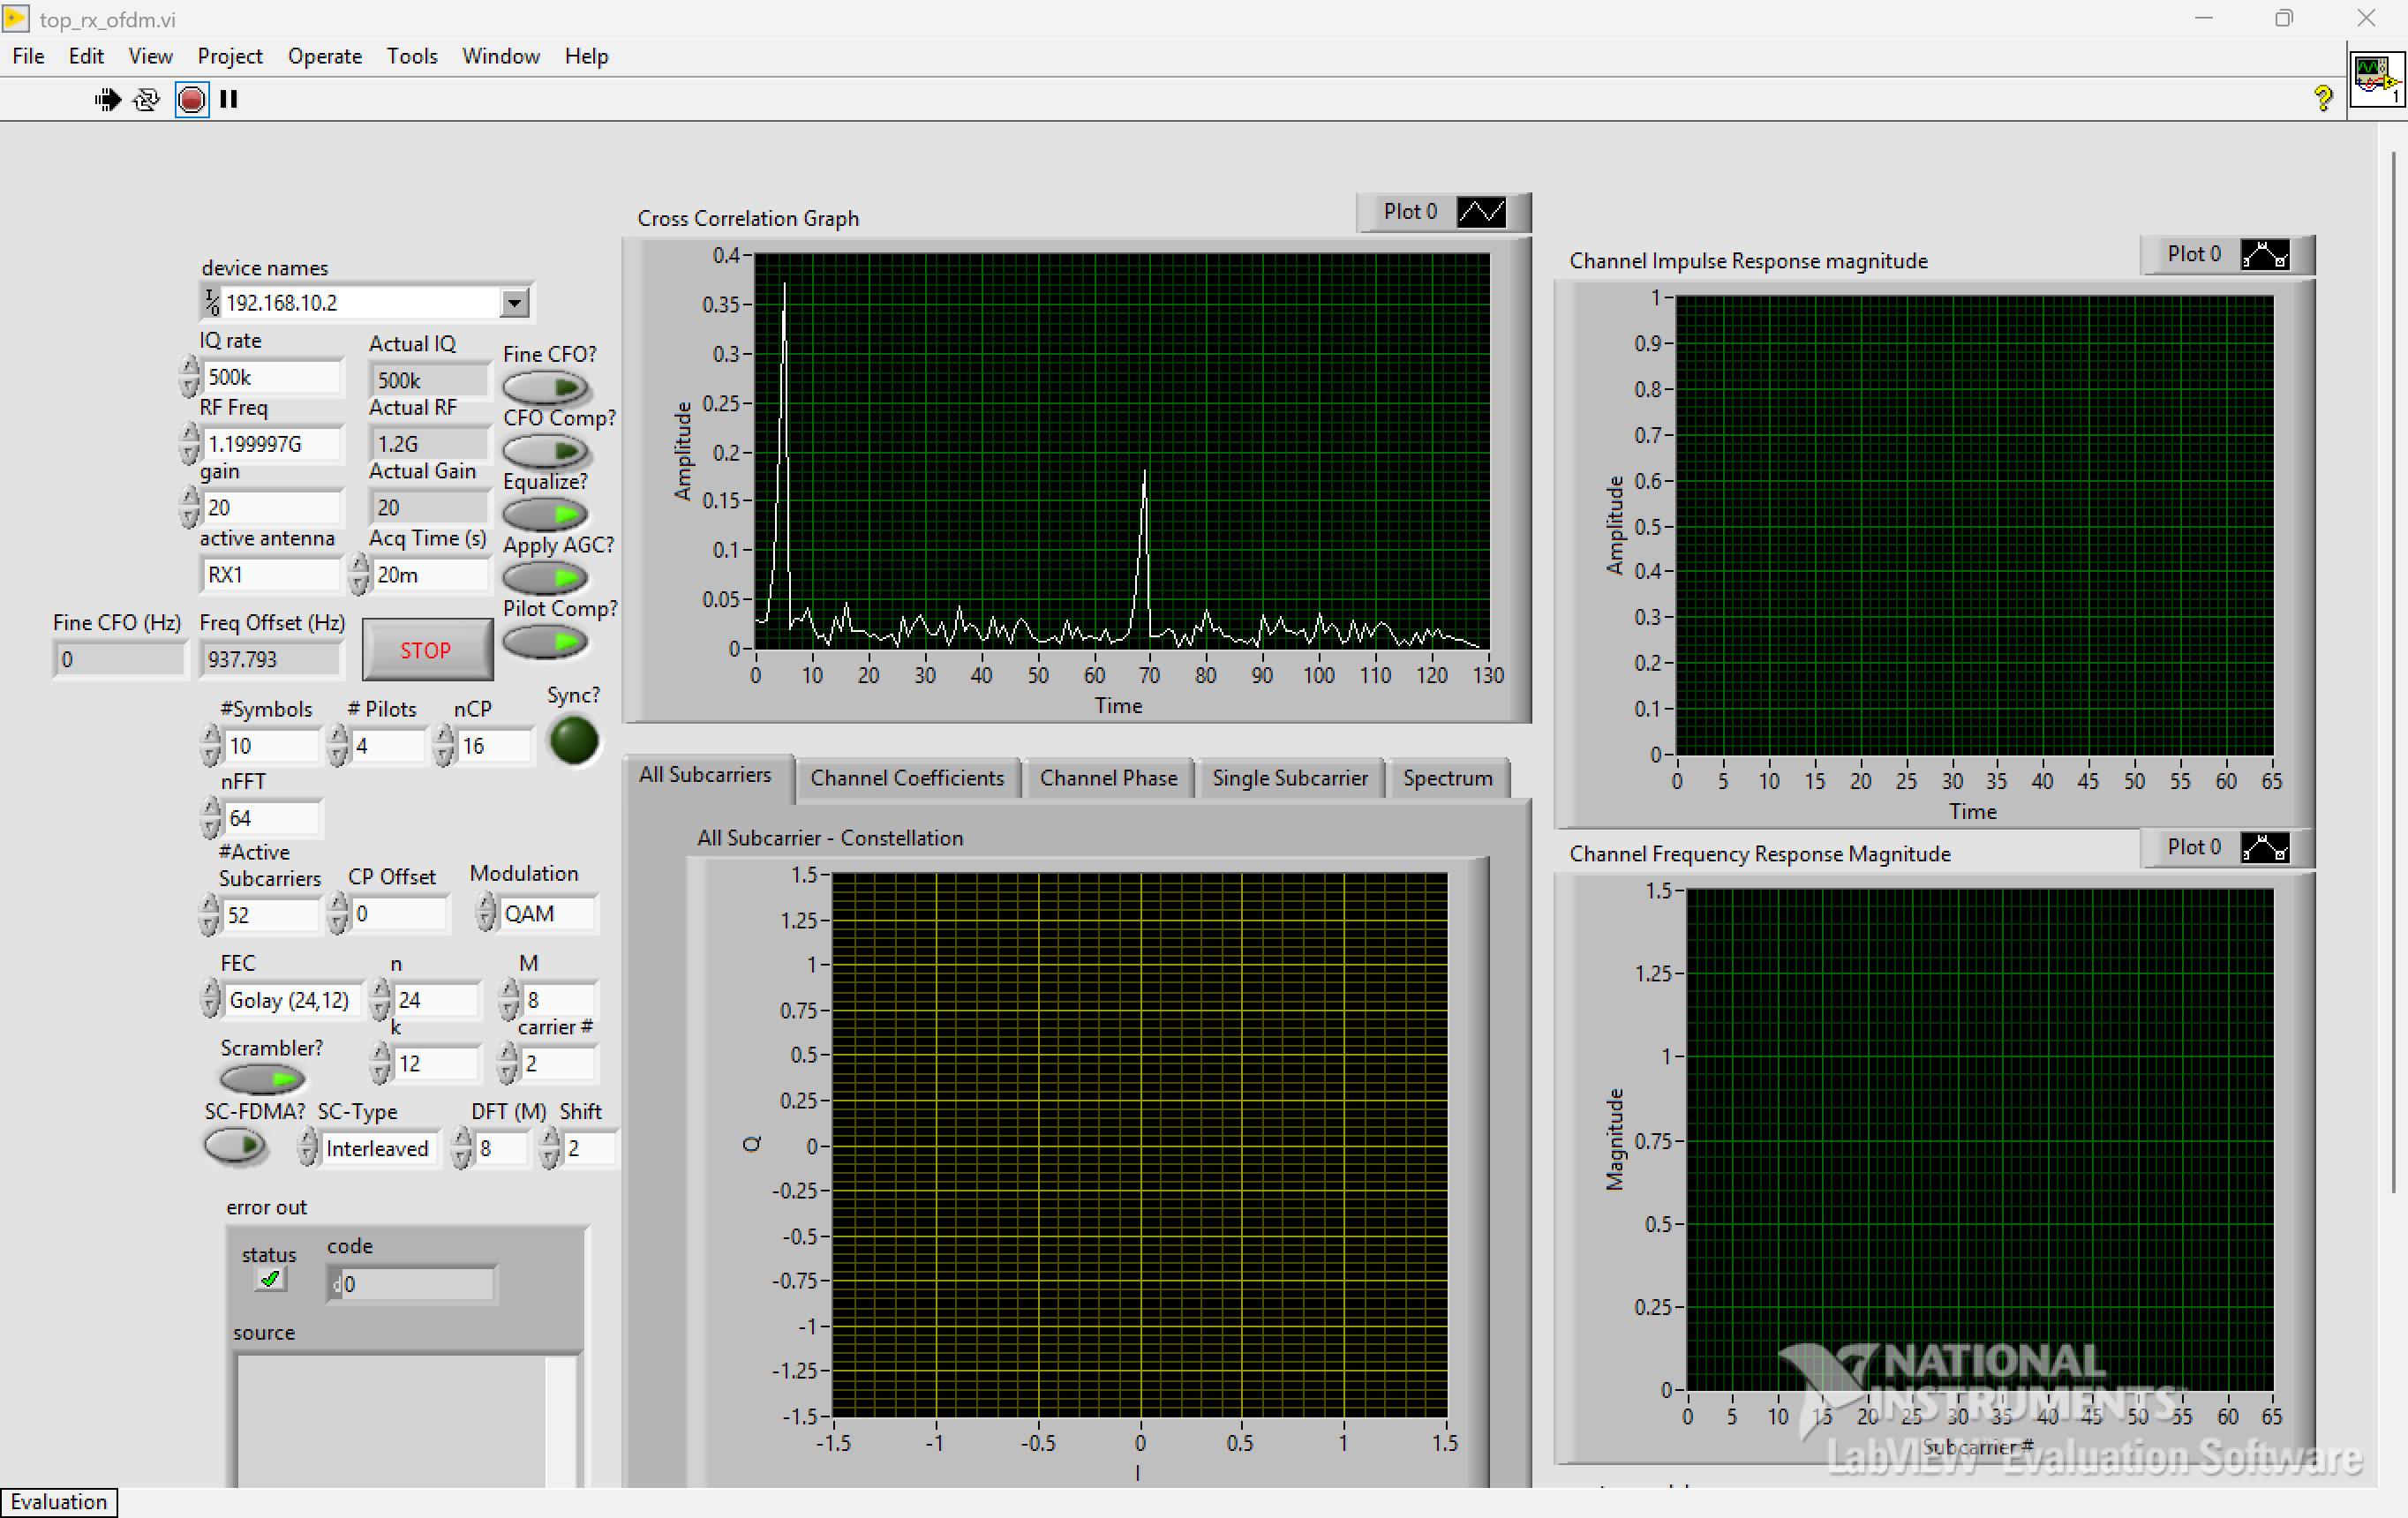
\includegraphics[width=0.7\textwidth]{lab_ss/WES268B_Lab7_Part3-2-4_3kHz-TotalToleration.png}
    \caption{Lab 7 - INSERT}
    %\label{f50}
\end{figure}

% 3.2.X
\subsubsection{ }

\noindent\textbf{Question.} 

\noindent\textbf{Answer.} 


% 4 Post Lab Questions
\section{Post Lab Questions}

\subsection{Post Lab Question 1}
INSERT

\subsection{Post Lab Question 2}
INSERT

\subsection{Post Lab Question 3}
INSERT

\subsection{Post Lab Question 4}
INSERT

% Easter Egg
\newpage
\thispagestyle{empty}
\vspace*{\fill}
\begin{center}
   
\includegraphics[width=0.4\textwidth]{EasterEgg2.png}\\[1em]
   \textbf{feelsgoodman}
\end{center}
\vspace*{\fill}

\end{document}
